% !TeX TS-program = lualatex

\documentclass[a4paper, 12pt, openany]{book}
%\usepackage[utf8]{inputenc}
\usepackage[italian]{babel}

\usepackage[]{csvsimple}
\usepackage{float}

\usepackage{ragged2e}
\usepackage[left=25mm, right=25mm, top=15mm]{geometry}
\geometry{a4paper}
\usepackage{graphicx}
\usepackage{booktabs}
\usepackage{paralist}
\usepackage{subfig} 
\usepackage{fancyhdr}
\usepackage{amsmath}
\usepackage{amssymb}
\usepackage{amsfonts}
\usepackage{amsthm}
\usepackage{mathtools}
\usepackage{enumitem}
\usepackage{titlesec}
\usepackage{braket}
\usepackage{gensymb}
\usepackage{url}
\usepackage{hyperref}
\usepackage{csquotes}
\usepackage{multicol}
\usepackage{graphicx}
\usepackage{wrapfig}
\usepackage{caption}

\usepackage{esint}

\captionsetup{font=small}
\pagestyle{fancy}
\renewcommand{\headrulewidth}{0pt}
\lhead{}\chead{}\rhead{}
\lfoot{}\cfoot{\thepage}\rfoot{}
\usepackage{sectsty}
\usepackage[nottoc,notlof,notlot]{tocbibind}
\usepackage[titles,subfigure]{tocloft}
\renewcommand{\cftsecfont}{\rmfamily\mdseries\upshape}
\renewcommand{\cftsecpagefont}{\rmfamily\mdseries\upshape}

\let\oldsection\section% Store \section
\renewcommand{\section}{% Update \section
	\renewcommand{\theequation}{\thesection.\arabic{equation}}% Update equation number
	\oldsection}% Regular \section
\let\oldsubsection\subsection% Store \subsection
\renewcommand{\subsection}{% Update \subsection
	\renewcommand{\theequation}{\thesubsection.\arabic{equation}}% Update equation number
	\oldsubsection}% Regular \subsection

\newcommand{\abs}[1]{\left\lvert#1\right\rvert}
\newcommand{\norm}[1]{\left\lVert#1\right\rVert}
\newcommand{\vprod}[2]{\vec{#1}\times\vec{#2}}
\newcommand{\sprod}[2]{\vec{#1}\cdot\vec{#2}}

\newcommand{\g}{\text{g}}
\newcommand{\m}{\text{m}}
\newcommand{\cm}{\text{cm}}
\newcommand{\mm}{\text{mm}}
\newcommand{\s}{\text{s}}
\newcommand{\N}{\text{N}}
\newcommand{\Hz}{\text{Hz}}

\newcommand{\virgolette}[1]{``\text{#1}"}
\newcommand{\tildetext}{\raise.17ex\hbox{$\scriptstyle\mathtt{\sim}$}}

\renewcommand{\arraystretch}{1.2}

\addto\captionsenglish{\renewcommand{\figurename}{Fig.}}
\addto\captionsenglish{\renewcommand{\tablename}{Tab.}}

\DeclareCaptionLabelFormat{andtable}{#1~#2  \&  \tablename~\thetable}

\setlength{\parindent}{0pt}

\newcommand{\dive}{\nabla\cdot}
\newcommand{\rot}{\nabla\times}

\graphicspath{{./images/}}

% feynman diagrams
\usepackage[compat=1.1.0]{tikz-feynman}

\author{Leonardo Cerasi%
	\thanks{\scriptsize\href{mailto:leonardo.cerasi@studenti.unimi.it}{leo.cerasi@pm.me}}%
	, Lucrezia Bioni\\
	\small GitHub repository: \href{https://github.com/LeonardoCerasi/notes}{LeonardoCerasi/notes}}

\title{\Huge\textbf{Fisica Nucleare e Subnucleare} \\ \large Prof.ssa S. Leoni, a.a. 2024-25}

\begin{document}

\frontmatter

\maketitle

\tableofcontents
\pagestyle{indice}

\mainmatter

\chapter*{Introduzione}
\pagestyle{introd}
\addcontentsline{toc}{chapter}{Introduzione}
\markboth{Introduzione}{}
\selectlanguage{italian}

Il problema generale che si va ad analizzare è il sistema di $ N_n $ elettroni ed $ N_n $ nuclei atomici, il cui moto non-relativistico è affetto solo dall'interazione elettromagnetica ed è dunque descritto dall'Hamiltoniana:
\begin{equation*}
	\mathcal{H} = T_n + T_e + V_{ne} + V_{nn} + V_{ee}
\end{equation*}
L'energia cinetica totale dei nuclei è:
\begin{equation*}
	T_n = \frac{1}{2} \sum_\alpha \frac{\ve{P}_{\ve{R}_\alpha}^2}{M_\alpha}
\end{equation*}
dove $ \ve{P}_{\ve{R}_\alpha} $ è il momento coniugato alla posizione $ \ve{R}_\alpha $ dell'$ \alpha $-esimo nucleo, mentre l'energia cinetica degli elettroni è:
\begin{equation*}
	T_e = \frac{1}{2m_e} \sum_i \ve{P}_{\ve{r}_i}^2
\end{equation*}
dove $ \ve{P}_{\ve{r}_i} $ è il momento coniugato alla posizione $ \ve{r}_i $ dell'$ i $-esimo elettrone. I potenziali d'interazione elettromagnetica sono invece:
\begin{equation*}
	V_{ne} = - \frac{q_e^2}{4\pi \epsilon_0} \sum_\alpha \sum_i \frac{Z_\alpha}{\abs{\ve{R}_\alpha - \ve{r}_i}}
\end{equation*}
\begin{equation*}
	V_{nn} = \frac{q_e^2}{4\pi \epsilon_0} \frac{1}{2} \sum_\alpha \sum_{\beta \neq \alpha} \frac{Z_\alpha Z_\beta}{\abs{\ve{r}_\alpha - \ve{r}_\beta}}
\end{equation*}
\begin{equation*}
	V_{ee} = \frac{q_e^2}{4\pi \epsilon_0} \frac{1}{2} \sum_i \sum_{j \neq i} \frac{1}{\abs{\ve{r}_i - \ve{r}_j}}
\end{equation*}
La risoluzione analitica di questo problema è possibile solo in un numero limitato di casi, mentre la sua integrazione numerica scala in complessità esponenzialmente con $ N = N_e + N_n $.\\
Nella formulazione di tale Hamiltoniana, si sono applicate alcune approssimazioni:
\begin{enumerate}
	\item corpi puntiformi: mentre per l'elettrone, in quanto particella fondamentale, questa assunzione è sempre lecita, per il nucleo atomico essa è possibile visto che il rapporto tra raggio nucleare e raggio atomico è dell'ordine di $ 10^{-3} $, oltre al fatto che le energie in gioco nei processi atomici ($ \sim 1\ev $) non sono sufficienti ad eccitare i gradi di libertà interni del nucleo ($ \sim 1\mev $);
	\item moto non-relativistico: alcune correzioni relativistiche (es.: interazione spin-orbita) possono essere trattate perturbativamente;
	\item sistema isolato: si assume il sistema non-interagente con l'ambiente esterno ed in assenza di campi esterni.
\end{enumerate}
Si noti che mentre i sistemi a singola particella godono di determinate simmetrie, quelli a molti corpi possono presentare delle rotture spontanee di simmetria: ciò è particolarmente evidente nei sistemi molecolari, mentre in quelli atomici è presente ma in misura minore, ed avviene poiché nei casi in cui una rottura di simmetria permetta di abbassare l'energia totale del sistema.

\paragraph{Ordini di grandezza}

Innanzitutto, conviene definire la coupling constant dell'interazione elettromagnetica:
\begin{equation*}
	e^2 \equiv \frac{q_e^2}{4\pi \epsilon_0} = 2.3071 \cdot 10^{-28} \,\text{J} \,\text{m} = 14.3387 \ev \ang
\end{equation*}
La scala del moto elettronico nell'atomo è data dal \textit{raggio di Bohr}:
\begin{equation*}
	a_0 \equiv \frac{\hbar^2}{m_e e^2} = 0.529177 \cdot 10^{-10} \,\text{m} = 0.529177 \ang
\end{equation*}
Evidenze sperimentali mostrano che gli atomi nella materia sono distanziati nell'ordine di $ 2a_0 - 10a_0 $. La scala delle interazioni elettromagnetiche in ambito atomico/molecolare è dunque data dall'\textit{energia di Hartree}:
\begin{equation*}
	E_\text{Ha} \equiv \frac{e^2}{a_0} = 4.35974 \cdot 10^{-18} \,\text{J} = 27.2114 \ev
\end{equation*}
La tipica timescale del moto elettronico si ottiene dal principio d'indeterminazione:
\begin{equation*}
	t_0 = \frac{\hbar}{E_\text{Ha}} = 2.4189 \cdot 10^{-17} \,\text{s}
\end{equation*}
Ciò permette di calcolare la scala delle velocità elettroniche, confermando l'approssimazione non-relativistica:
\begin{equation*}
	v_0 = \frac{a_0}{t_0} = 2.1877 \cdot 10^6 \,\text{m} \,\text{s}^{-1} \simeq 0.01 c
\end{equation*}
La scala dei fenomeni relativistici nella dinamica elettronica è data dalla \textit{costante di struttura fine}:
\begin{equation*}
	\alpha = \frac{v_0}{c} = \frac{e^2}{\hbar c} = 7.29734 \cdot 10^{-3} \simeq \frac{1}{137.036}
\end{equation*}
Comparando con le onde elettromagnetiche, la scala delle distanze interatomiche ($ \sim 1\ang $) corrisponde alla regione dei raggi X, mentre quella delle frequenze elettroniche (e dunque di $ E_\text{Ha} $) corrisponde alla fascia UV ($ \lambda \sim 10^3 a_0 $); le frequenze tipiche (e dunque le energie) del moto nucleare sono invece associate alla regione IR ($ \nu \sim 5 \,\text{THz} $).

\paragraph{Spettroscopia}

Gli esperimenti spettroscopici sono quelli in cui una proprietà caratterizzante l'interazione tra radiazione e materia è misurata in funzione della frequenza della radiazione incidente sul campione che si vuole studiare. I principali tipi di spettroscopia sono due:
\begin{enumerate}
	\item assorbimento: un fascio collimato di luce monocromatica incide sul bersaglio; se la frequenza della radiazione coincide con quella di una transizione specifica del campione, ci sarà un importante assorbimento di fotoni: questo sarà visibile plottando l'intensità della radiazione emergente dal campione $ I(\omega) $, ottenendo il cosiddetto spettro d'assorbimento;
	\item emissione: il campione viene portato in uno stato eccitato (es.: bombardandolo di elettroni o fotoni alto-energetici), dunque emetterà della radiazione ad ogni transizione di diseccitamento, la quale va a formare il cosiddetto spettro d'emissione.
\end{enumerate}
Gli spettri atomici e molecolari sono dunque caratterizzati da picchi monocromatici, detti linee, associate a transizioni risonanti tra stati $ \ket{i} , \ket{f} $ che determinano linee a $ \omega_{if} = \frac{1}{\hbar} \abs{E_i - E_f} $. Sebbene a livello teorico queste linee sarebbero delle $ \delta $ di Dirac, sperimentalmente si misurano sempre delle righe più o meno strette; le cause dell'allargamento delle linee spettrali sono sia intrinseche che estrinseche, e principalmente sono:
\begin{enumerate}
	\item risoluzione sperimentale: tipicamente determinata da vari effetti aleatori, dunque determina una forma gaussiana; può essere migliorata con accorgimenti tecnici;
	\item allargamento naturale: dovuto al fatto che gli stati eccitati, sebbene stazionari in prima approssimazione, vengono resi instabili dall'interazione col le fluttuazioni di punto-zero del campo elettromagnetico (quantistico); si determina dunque un decadimento spontaneo di tutti gli autostati d'energia (eccetto il ground state) che, sebbene randomico per un singolo atomo, segue una legge statistica per un sistema a molti atomi:
	\begin{equation*}
		N(t) = N_0 e^{- \gamma t} = N_0 e^{- t / \tau}
	\end{equation*}
	dove $ \gamma $ è la costante di decadimento e $ \tau $ la vita media dello stato eccitato, la quale setta la durata tipica della spettroscopia. Dal principio d'indeterminazione, si trova che l'energia di uno stato eccitato non è misurabile con precisione migliore di:
	\begin{equation*}
		\Delta E = \frac{\hbar}{\tau} = \hbar \gamma
	\end{equation*}
	Ciò causa dunque l'allargamento naturale delle linee spettrali secondo la Lorentziana:
	\begin{equation*}
		I(\omega) = I_0 \frac{\gamma^2}{(\omega - \omega_{if})^2 + \gamma^2}
	\end{equation*}
	Gli stati atomici eccitati hanno $ \tau \sim 1\,\text{ns} $, dunque l'allargamento è di $ \Delta E \sim 1\,\mu\text{eV} $.
	\item allargamento Doppler: nel caso di un campione in fase gassosa, il moto termico randomico degli atomi/molecole determina un red/blue-shift delle frequenze di transizione, a seconda della velocità casuale dell'atomo/molecola che decade; si ha un allargamento gaussiano delle righe spettrali, che determina:
	\begin{equation*}
		\Delta \omega_\text{Doppler} = \omega_{if} \sqrt{8 \ln(2) \frac{k_B T}{M c^2}}
	\end{equation*}
	A temperatura fissata, gli atomi/molecole più leggeri si muoveranno più velocemente, determinando un allargamento maggiore (sempre nell'ordine dei $ \mu\text{eV} $).
\end{enumerate}
Si ha dunque un allargamento totale pari alla somma in quadratura di questi allargamenti singoli.












\part{Fisica Nucleare}
\pagestyle{body}

\chapter{Nuclidi}
\pagestyle{body}
\selectlanguage{italian}
\section{Definizioni e nomenclatura}

Un nuclide (o nucleo) è una specifica combinazione di protoni e neutroni: si definiscono il numero atomico $ Z $ come il numero di protoni, il numero di neutroni $ N $ ed il numero di massa $ A = Z + N $ come il numero di nucleoni. In un atomo neutro, $ Z $ è anche il numero totale di elettroni negli orbitali.\\
Il simbolo completo di un nuclide è $ ^A_Z \text{X}_N $, dove $ \text{X} $ è il simbolo della specie chimica: tale scrittura è però ridondante, poiché la specie chimica definisce di per sé il numero di protoni nel nuclide, dunque è sufficiente scrivere $ ^A \text{X} $.\\
Nuclidi con lo stesso $ Z $ sono detti isotopi, con lo stesso $ A $ isobari e con lo stesso $ N $ isotoni.

\subsection{Unità di misura}

Nell'ambito della fisica nucleare e particellare è sconveniente utilizzare le unità di misura del Sistema Internazionale: unità di misura tipiche sono il fermi $ 1\fm = 10^{-15}\m $, l'elettronvolt $ 1\ev = 1.602\cdot10^{-19}\,\text{J} $ e l'unità di massa atomica $ 1\,\text{u} = 1.6606\cdot10^{-27}\,\text{kg} = 931.502 \mev/c^2 $ (definita come $ 1/12 $ della massa di un atomo di $ \ch{^{12}C} $).\\
Per semplificare le equazioni, è utile porre le costanti fondamentali $ c = \hbar = 1 $: questo sistema di misura è detto Sistema Naturale e in esso massa, momento lineare, energia, lunghezza$ ^{-1} $ e tempo$ ^{-1} $ hanno la stessa unità di misura, poiché le equazioni di Einstein, Plank e de Broglie diventano rispettivamente $ E^2 = m_0^2 + p^2 $, $ E = 2\pi \nu $ e $ \lambda = \frac{2\pi}{p} $.

\subsubsection{Masse e costanti}

Nel SI, è utile ricordare i seguenti valori approssimati delle costanti fondamentali:
\begin{equation*}
    \begin{split}
	  &c = 2.99792458\cdot10^8 \m/\text{s} \approx 3\cdot10^8 \m/\text{s}\\
	  &\hbar = 6.58211928\cdot10^{-22} \mev\,\text{s} \approx \frac{2}{3}\cdot10^{-21} \mev\,\text{s}\\
	  &\hbar c = 197.3269718 \mev\fm \approx 200 \mev\fm
    \end{split}
\end{equation*}

Si possono quindi esprimere le masse dei nucleoni e dell'elettrone in varie unità di misura:
\begin{equation*}
	\begin{split}
		&m_p = 1.673\cdot10^{-27}\,\text{kg} = 1.00728\,\text{u} = 938.279 \mev/c^2\\
		&m_n = 1.675\cdot10^{-27}\,\text{kg} = 1.00867\,\text{u} = 939.573 \mev/c^2\\
		&m_e = 9.110\cdot10^{-31}\,\text{kg} = 0.511\mev/c^2
	\end{split}
\end{equation*}

Parametro utile:
\begin{equation*}
	\begin{split}
		&e^2 = 1.440 \cdot 10^{-15} \mev/m = 1.440 \mev\cdot \fm
	\end{split}
\end{equation*}

\subsection{La tavola di Segré}

Al pari delle specie chimiche nella tavola periodica, anche i nuclidi possono essere messi in una tabella, tipicamente in un piano $ Z - N $ (Fig. \ref{segre-chart}): questa viene detta tavola di Segré e permette di tracciare facilmente i vari decadimenti radioattivi dei nuclidi, visualizzando efficaciemente le decay chains.\\
Come si vede in Fig. \ref{drip-lines}, è possibile distinguere la tavola dei nuclidi in due regioni separate da due linee: queste sono dette nuclear driplines e distinguono tra configurazioni di protoni e neutroni che possono effettivamente formare dei nuclidi (sia stabili che instabili, ovvero radioattivi) e configurazioni nelle quali invece l'interazione forte non riesce a mantenere insieme i nucleoni per formare un nucleo. Si stima che possano esistere oltre $ 7000 $ nuclidi nell'Universo, ma di questi solo circa $ 3000 $ sono stati effettivamente scoperti (di cui solo $ 251 $ nuclidi stabili): si parla in questo caso di $ \virgolette{Terra incognita} $ per indicare il teoricamente alto numero di nuclidi ancora ignoti; in particolare, è stata teoricamente prevista un'$ \virgolette{isola} $ di elementi super-pesanti attorno a $ Z = 114 $ ed oltre, con nuclidi con vite medie dell'ordine di minuti o giorni: sebbene non ancora osservati, si pensa che la chimica degli elementi super-pesanti con $ Z > 118 $ sia di natura relativistica, dunque incomparabile a quella degli elementi fin'ora scoperti. \\
La carta dei nuclidi, inoltre, fornisce importanti informazioni su come avvenngono i decadimenti radioattivi:
\begin{enumerate}
	\item se ci si sposta lungo la bisettrice del II e del IV quadrante si hanno i \virgolette{decadimenti beta}, caratterizzati dall'aumento/diminuzione del numero di protoni e dalla diminuzione/aumento del numero di neutroni;
	\item se ci si sposta lungo la bisettrice del I e del III quadrante si ha una diminuzione/aumento sia del numero di protoni sia del numero di neutroni. Poiché la carica si deve conservare, si ha anche una diminuzione/aumento del numero di massa di 2. Il \virgolette{decadimento alfa} corrisponde a 2 spostamenti a sinistra e due in basso.
  \end{enumerate}

\begin{figure}
  \centering
  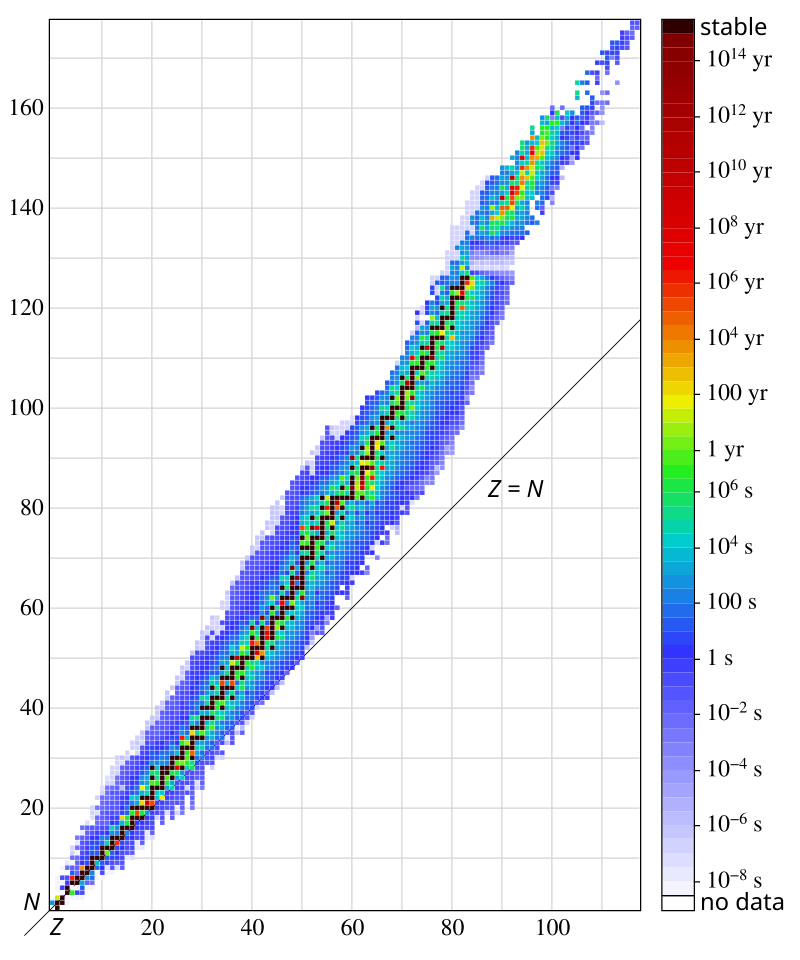
\includegraphics[width = 0.75\textwidth]{segre-chart.png}
  \caption{Tavola di Segré.}
  \label{segre-chart}
\end{figure}
\begin{figure}
  \centering
  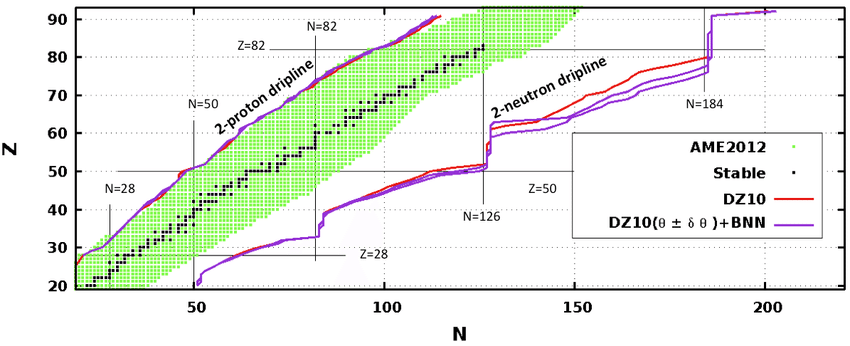
\includegraphics[width = 0.55\textwidth]{drip-lines.png}
  \caption{Nuclear driplines.}
  \label{drip-lines}
\end{figure}

\section{Evidenze sperimentali}

Le prime evidenze sperimentali dell'esistenza del nucleo atomico si devono al gruppo di ricerca di Rutherford, Geiger e Marsden: prima di loro, Thomson era riuscito ad estrarre delle cariche negative dall'atomo, identificando l'elettrone, ed aveva di conseguenza formulato la sua teoria della struttura atomica come sfera carica positivamente in cui sono immersi gli elettroni ($ \virgolette{plum pudding} $ model).\\
Con i loro esperimenti, Rutherford et al. dimostrarono invece che le cariche positive erano concentrate in una regione piccola al centro dell'atomo.

\subsection{Scattering di Rutherford}

L'esperimento condotto da Rutherford et al. consiste nell'irradiare una lamina sottile di oro con un fascio collimato di particelle $ \alpha $ (nuclei di $ \ch{^{4} He} $). Rutherford non aveva a disposizione acceleratori, e usò particelle $\alpha$ provenienti dai decadimenti radioattivi, con energie di pochi \mev, e dunque influenzate solo dall'interazione coulombiana. A livello puramente cinematico (ignorando la natura dell'interazione tra beam e target), essendo la velocità delle particelle $ \alpha $ $ v_0 \sim 0.1c $, è possibile trattare il problema come un urto elastico non-relativistico (conservazione della quantità di moto e dell'energia):
\begin{equation}
	\begin{cases}
	  m_{\alpha} \ve{v}_0 = m_{\alpha} \ve{v}_f + m_t \ve{v}_t \\
	  m_{\alpha} v_0^2 = m_{\alpha} v_f^2 + m_t v_t^2 \\
	\end{cases}
	\label{eq:2}
\end{equation}
Combinando le due equazioni e definendo $ \theta $ l'angolo tra $ \ve{v}_f $ e $ \ve{v}_t $ (velocità del target):
\begin{equation}
	\cos \theta = \frac{1}{2} \frac{v_t}{v_f} \left(1 - \frac{m_t}{m_{\alpha}}\right)
	\label{eq:3}
\end{equation}
Si possono distinguere due principali casi:
\begin{enumerate}
	\item $ m_t = m_e \ll m_{\alpha} $: $ \cos \theta > 0 $: la particella colpisce l'elettrone, e si parla di forward scattering, poiché non sono possibili grossi valori di $ \theta $ (deflessione) e la particella viene trasmessa attraverso il materiale;
	\item $ m_t = m_{Au} \gg m_{\alpha} $: $ \cos \theta < 0 $: urto tra oggetti massicci, dunque diventano possibili anche angoli di deviazione della traiettoria della particella $\alpha$ prossimi $ \pi $, e il rinculo del nucleo.
\end{enumerate}
Il modello di Thomson rientra nella prima casistica, poiché in tal caso all'interno dell'atomo lo scattering può avvenire solo con gli elettroni, che hanno $ m_e = 0.511 \mev/c^2 \ll m_{\alpha} = 4 \gev/c^2 \approx 4m_p , \frac{m_e}{m_{\alpha}} \approx 10^{-4} $. Questo implica che la massima quantità di moto trasferita al bersaglio elettronico è $\approx 10^{-4} p_i$, ovvero un piccolo cambiamento nella quantità di moto della particella $\alpha$.\\
Ciò che Rutherford et al. osservarono, però, è che occasionalmente delle particelle $ \alpha $ vengono riflesse dalla lamina d'oro: questo risultato è incompatibile con lo scattering con elettroni o con una carica positiva diffusa, dunque fu confermato che la carica positiva nell'atomo è concentrata in un unico punto massivo, il nucleo atomico. Infatti, $\frac{m_{Au-197}}{m_{\alpha}}\approx 50$, dove $m_{Au-197}=197 \gev/c^2$, ovvero il target è molto più massivo del proiettile. Questo implica che il nucleo può sottrarre fino al doppio del momento incidente, e la particella $\alpha$ può tornare indietro con una quantità di moto uguale e opposta a quella iniziale.

\subsubsection{Cross-section di Rutherford}

Nella trattazione cinematica è stata ignorata l'interazione tra particelle $ \alpha $ e nucleo atomico, che è ciò che effettivamente determina lo scattering: essa può essere modellata, in forma approssimativa (in particolare per parametro d'urto compreso tra il raggio nucleare e l'orbita elettronica più interna), dal potenziale coulombiano. Si assumono particelle puntiformi, poiché $\alpha$ non può penetrare nel nucleo. Dette $ Z $ il numero atomico dell'atomo target e $ Z' $ quello degli atomi del beam (nel caso specifico dello scattering di Rutherford $ Z = Z_{\ch{Au}} = 79 $ e $ Z' = Z_{\ch{He}} = 4 $), il potenziale d'interazione è:
\begin{equation}
	V(\ve{r}) = \frac{ZZ' e^2}{r}
	\label{eq:4}
\end{equation}
Dalla meccanica classica è possibile legare il parametro d'urto $ b $ all'angolo di scattering $ \theta $:
\begin{equation}
	b = \frac{ZZ' e^2}{2 E_0} \cot \frac{\theta}{2}
	\label{eq:5}
\end{equation}
dove $ E_0 $ è l'energia della particella incidente.\\
È possibile stimare quanto vicino al nucleo atomico si possono spingere le particelle $ \alpha $ tramite la distanza di closest approach $ a $, definita dalla condizione $ V(a) = E_0 $ ed esprimibile anche in funzione di $ b $ e $ \theta $ tramite $ \tan \frac{\theta}{2} = \frac{a}{2b} $: le particelle $ \alpha $ usate da Rutherford avevano $ E_{\alpha} \approx 5\mev $, dunque fu in grado di sondare il nucleo atomico poiché $ a \approx 45\fm $.\\
Per calcolare la cross-section dello scattering di Rutherford, si consideri un fascio incidente monoenergetico con energia $ E_0 $ e $ N_0 $ particelle incidenti per unità di area e di tempo: facendo variare il parametro d'urto tra $ b $ e $ b + db $, dunque variando l'angolo di scattering tra $ \theta $ e $ \theta - d \theta $, si avranno $ 2\pi N_0 b \,db $ particelle incidenti per unità di tempo (data la sezione d'urto $ \Delta\sigma = 2\pi b \,db $, Fig. \ref{rutherford}).
\begin{figure}
	\centering
	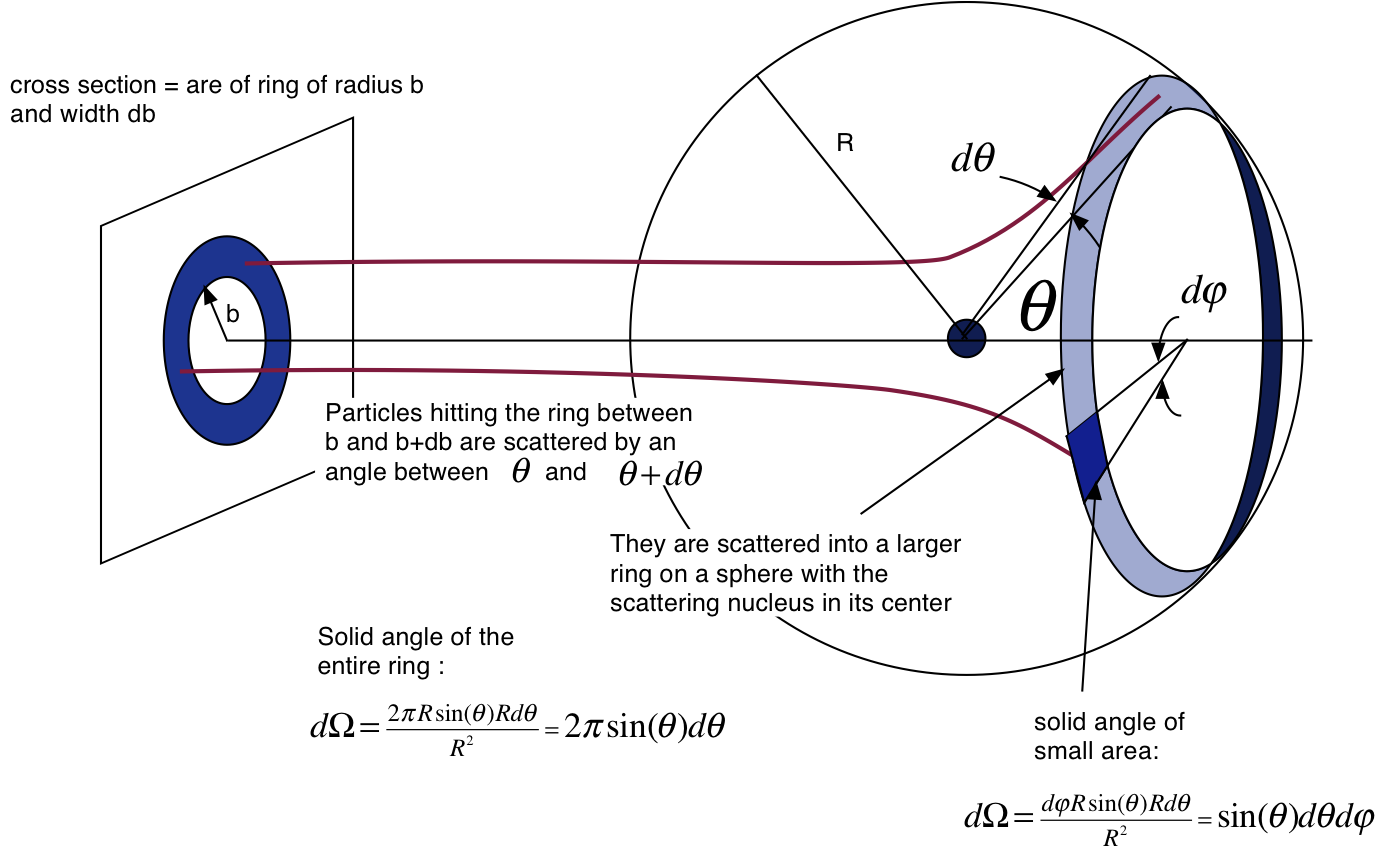
\includegraphics[width=0.95\textwidth]{rutherford.png}
	\caption{Sezione d'urto dello scattering di Rutherford.}
	\label{rutherford}
\end{figure}

Va notato che è possibile ignorare il fatto che la lamina target ha un numero elevato di atomi target e che ogni particella nel beam incidente ha un diverso parametro d'urto relativo a ciascuno di essi, poiché la lastra è considerata così sottile da rendere improbabili collisioni multiple della stessa particella incidente; inoltre, dal modello atomico di Rutherford ricaviamo che i nuclei atomici si trovano a distanze grandi rispetto alle loro dimensioni, rendendo significative solo le traiettorie con parametro d'urto vicino al nucleo atomico.\\
Nel caso di un potenziale d'interazione generico, $ \Delta\sigma $ può avere anche dipendenza azimuthale:
\begin{equation}
	\Delta\sigma(\theta,\phi) = b \,db\,d\phi = - \frac{d\sigma}{d\Omega} (\theta,\phi) \,d\Omega= - \frac{d\sigma}{d\Omega} (\theta,\phi) \sin \theta \,d\theta\,d\phi
	\label{eq:6}
\end{equation}
dov'è stata utilizzata la differential cross-section $ \frac{d\sigma}{d\Omega} $ e dove si è tenuto conto che un aumento di $ b $ porta ad una diminuzione di $ \theta $ tramite il segno negativo.\\
Essendo il potenziale coulombiano un potenziale centrale a simmetria sferica, è possibile semplificare il calcolo grazie alla simmetria azimuthale, ottenendo:
\begin{equation}
	\frac{d\sigma}{d\Omega} (\theta) = - \frac{b}{\sin \theta} \frac{db}{d\theta}
	\label{eq:7}
\end{equation}
Lo scattering di Rutherford può essere quindi completamente caratterizzato utilizzando l'Eq. \ref{eq:5}:
\begin{equation}
	\frac{d\sigma}{d\Omega} (\theta) = \left( \frac{ZZ' e^2}{4 E_0} \right)^2 \frac{1}{\sin^4 \frac{\theta}{2}}
	\label{eq:8}
\end{equation}
È anche possibile definire la sezione d'urto totale $ \sigma_{\text{tot}} $ come:
\begin{equation}
	\sigma_{\text{tot}} = \int_{\Omega} \frac{d\sigma}{d\Omega} (\theta,\phi) \,d\Omega
	\label{eq:9}
\end{equation}
Essa rappresenta una sorta di area di scattering effettiva che la sorgente del potenziale determina a tutti i possibili valori del parametro d'urto.\\
Nel caso dello scattering di Rutherford:
\begin{equation}
	\begin{split}
		\sigma_{\text{tot}} &= \int_0^{2\pi} \int_0^{\pi} \frac{d\sigma}{d\Omega} (\theta,\phi) \sin \theta \,d\theta\,d\phi = 2\pi \int_0^{\pi} \frac{d\sigma}{d\Omega} (\theta) \sin \theta \,d\theta \\
				    &= 8\pi \left( \frac{ZZ' e^2}{4 E_0} \right)^2 \int_0^1 \frac{1}{\sin^3 \frac{\theta}{2}} d\left( \sin \frac{\theta}{2} \right) \longrightarrow \infty
	\end{split}
	\label{eq:10}
\end{equation}
Questo risultato divergente è coerente con l'interpretazione data della sezione d'urto totale: il potenziale coulombiano è associato all'interazione elettromagnetica, la quale ha un range infinito, dunque anche l'area efficace di scattering sarà infita.\\
In maniera realistica, però, si può considerare che dopo un determinato valore di cutoff $ b_0 $ lo scattering non abbia più effetti osservabili sulla particella incidente, dunque la sezione d'urto totale osservabile si ottiene integrando la differential cross-section tra $ 0 $ e $ \theta_0 < \pi$, ottenendo dunque un valore finito.\\
La formula di Rutherford \ref{eq:8} cessa di essere valida quando $ E_0 $ diventa troppo alta, in particolare quando la particella $ \alpha $ riesce a penetrare nel nucleo, poiché a quel punto subentrano l'interazione nucleare fin'ora ignorata: studiando sperimentalmente a quale energia (a differenti angoli di scattering) si iniziano a manifestare le deviazioni dalla cross-section di Rutherford, è possibile stimare il raggio nucleare tramite la distanza di closest approach $ a $, trovando il fit sperimentale $ R = R_0 A^{1/3} $ con $ R_0 = 1.4\fm $.

\subsection{Scattering elettronico}

Data la dualità onda-particella che risulta da una descrizione quanto-meccanica della materia, la sezione d'urto da scattering non sarà determinata soltanto dall'interazione coulombiana ma anche da effetti diffrattivi, evidenziati dal pattern di diffrazione in Fig. \ref{diffraction}: l'analogo ottico è la diffrazione da disco opaco, poiché il nucleo atomico assorbe nucleoni, con la dovuta differenza che la superficie del nucleo ha una determinata diffusività, la quale determina dei minimi non-nulli nello spettro di diffrazione.
\begin{figure}
	\centering
	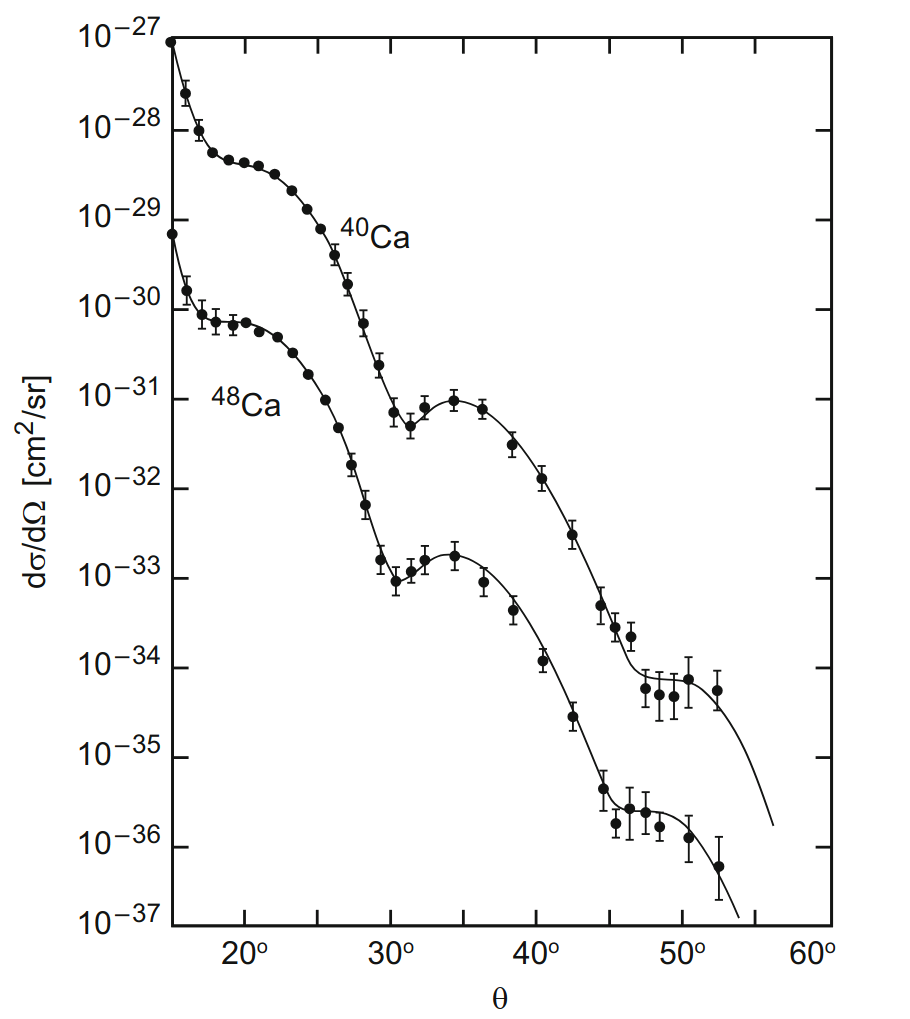
\includegraphics[width=0.95\textwidth]{diffraction.png}
	\caption{Sezione d'urto dello scattering elettronico.}
	\label{diffraction}
\end{figure}\\
Per evitare che all'interazione coulombiana si sovrapponga anche quella tra nucleoni, per studiare la struttura del nucleo atomico le sonde migliori sono gli elettroni: poiché per sondare una scala di lunghezze $ \Delta x $ è necessaria una lunghezza d'onda $ \lambda \sim \Delta x $, dalla relazione di de Broglie si ha che la quantità di moto degli elettroni incidenti deve essere $ p \sim h / \Delta x $. La struttura del nucleo atomico risulta visibile su scale di $ 1\fm $, dunque sono necessari elettroni con momento lineare $ p \approx 200 \mev/c $; nel caso si voglia studiare la struttura interna dei nucleoni, la stima aumenta di almeno un ordine di grandezza.\\
Va ricordato che gli elettroni, in quanto particelle cariche, quando percorrono una traiettoria curva irraggiano, dunque per questo tipo di scattering sono necessari accelleratori lineari.
Ricordando che $ E^2 = p^2 c^2 + m_0^2 c^4 $ ed $ E = K + m_0 c^2 $, considerando che $ m_e = 0.511 \mev/c^2 $, si vede che gli elettroni utilizzati per sondare il nucleo atomico sono in regime ultra-relativistico, dunque nel calcolo della cross-section sono da tenere in conto effetti relativistici legati allo spin ed il nuclear recoil (ovverosia il rinculo subito dal nucleo atomico a seguito dello scattering): trascurando quest'ultimo, si può applicare una correzione alla cross-section di Rutherford, detta cross-section di Mott:
\begin{equation}
	\left(\frac{d\sigma}{d\Omega}\right)_{\text{Mott}} = \left(\frac{d\sigma}{d\Omega}\right)_{\text{Ruth}} \left(1 - \beta^2 \sin^2 \frac{\theta}{2}\right)
	\label{eq:11}
\end{equation}
Queste sezioni d'urto, però, considerano scattering tra oggetti puntiformi, ma mentre un elettrone può effettivamente essere considerato tale, lo stesso non si può dire per il nucleo atomico, il quale avrà una certa distribuzione di carica $ \rho(\ve{r}) $ estesa nello spazio (essa coincide con la distribuzione di massa solo per nuclidi stabili); per considerare anche questo fatto, nel calcolo della cross-section si applica un'ulteriore correzione:
\begin{equation}
	\frac{d\sigma}{d\Omega} = \left(\frac{d\sigma}{d\Omega}\right)_{\text{Mott}} \abs{F(q)}^2
	\label{eq:12}
\end{equation}
dove $ \abs{F(q)}^2 $ è detto form factor e $ \ve{q} \defeq \frac{1}{\hbar} \abs{\ve{p}' - \ve{p}} $, con $ \ve{p} $ e $ \ve{p}' $ momento iniziale e finale dell'elettrone, esprime la variazione di quantità di moto dell'elettrone.\\
Dato che si sta considerando uno scattering elastico, si ha $ p = p' $ e dunque $ q = \frac{1}{\hbar} 2p \sin \frac{\theta}{2} $, con $ \theta $ angolo di scattering.\\
Nel caso dell'approssimazione di Born (elettroni come onde piane $ \psi(\ve{r}) = \frac{1}{\sqrt{V}} e^{i \ve{p}\cdot\ve{x} / \hbar} $) e trascurando il nuclear recoil, il form factor è la trasformata di Fourier della distribuzione di carica $ \rho(\ve{r}) $:
\begin{equation}
	F(q) = \int_{r \le R} e^{i \ve{p}\cdot\ve{r} / \hbar} \rho(\ve{r}) d^3\ve{r}
	\label{eq:13}
\end{equation}
con $ R $ raggio nucleare ed opportuna normalizzazione $ F(0) = 1 $.\\
In questa approssimazione, quindi, una misura della cross-section di scattering elettronico può dare informazioni sulla distribuzione di carica nel nucleo atomico; inoltre, è possibile dare una stima del raggio nucleare dallo studio dello spettro di diffrazione evidenziato dalla cross-section, poiché il primo minimo di diffrazione soddisfa la relazione $ \frac{q}{\hbar} \approx \frac{4.5}{R} $; se invece si considerano due isotopi, dal fatto che la separazione angolare tra due minimi è $ \Delta\theta = \frac{\hbar}{p R} $ si evince che all'aumentare del numero di massa aumenta anche il raggio nucleare (vedere Fig. \ref{diffraction}): ciò in generale è valido solo per nuclidi nella cosiddetta $ \virgolette{valle di stabilità} $, poiché per essi la distribuzione di neutroni segue quella di protoni, ovvero le distribuzioni ci carica e massa vanno a coincidere, dunque un nuclide con più nucleoni avrà un raggio nucleare maggiore; la difficoltà principale nella misura della distribuzione di nucleoni sta nel fatto che i neutroni sono trasparenti agli esperimenti di scattering, poiché non interagiscono né tramite interazione elettromagnetica né tramite interazione nucleare forte.

\subsubsection{Distribuzione di carica nucleare}

Compiendo esperimenti di scattering elettronico e raccogliendo dati relativi a vari nuclei atomici, si è giunti alla conclusione che i nuclidi non sono sfere con un confine ben delineato, ma al loro interno la densità di carica si mantiene approssimativamente costante, mentre verso la superficie essa si riduce su un intervallo radiale relativamente ampio; la distribuzione di carica nucleare può dunque essere approssimata da una distribuzione di Fermi:
\begin{equation}
	\rho(\ve{r}) = \frac{\rho_0}{1 + e^{(r - c) / a}}
	\label{eq:14}
\end{equation}
dove i parametri empirici valgono (per nuclei pesanti) $ c = 1.07\fm \cdot A^{1/3} $ e $ a = 0.54\fm $: $ c $ è il raggio nucleare a mezza altezza della distribuzione di carica, mentre $ a $ è la diffusività (ciò che rende la distribuzione smooth piuttosto che sharp).\\
Una volta nota la distribuzione di carica, è possibile calcolare il raggio quadratico medio: per nuclei medi e pesanti, si ha $ \sqrt{\langle r^2 \rangle} = 0.94\fm \cdot A^{1/3} $. Se si approssima il nucleo come una sfera uniformemente carica, il suo raggio, definito come raggio nucleare, è dato da $ R^2 = \frac{5}{3} \langle r^2 \rangle $, ovvero:
\begin{equation}
	R = 1.21\fm \cdot A^{1/3}
	\label{eq:14-bis}
\end{equation}
che è la definizione più diffusa di raggio nucleare.\\
È anche possibile definire una skin depth (o surface thickness) $ t $ come lo spessore del guscio sferico in cui la densità di carica diminuisce dal $ 90\% $ al $ 10\% $ del suo valore massimo: per nuclei pesanti, si trova $ t = 2a\ln9 \approx 4.4 a $.\\
Come si può vedere in Fig. \ref{charge-distr}, la densità di carica centrale $ \rho_0 $ diminuisce leggermente all'aumentare del numero di massa; se però viene considerata la presenza di neutroni e si moltiplica per un fattore $ A / Z $, si trova un valore quasi identico per tutti i nuclidi (questo è coerente con $ R \sim A^{1/3} $, poiché così $ \rho_0 \sim A / \text{Vol} $ rimane costante): questo corrisponde alla densità che teoricamente avrebbe della materia nucleare infinitamente estesa, pari a $ \rho_n \approx 0.17 \,\text{nucleoni} / \text{fm}^3 $, che corrisponde a $ c = 1.12\fm \cdot A^{1/3} $.
\begin{figure}[!ht]
	\centering
	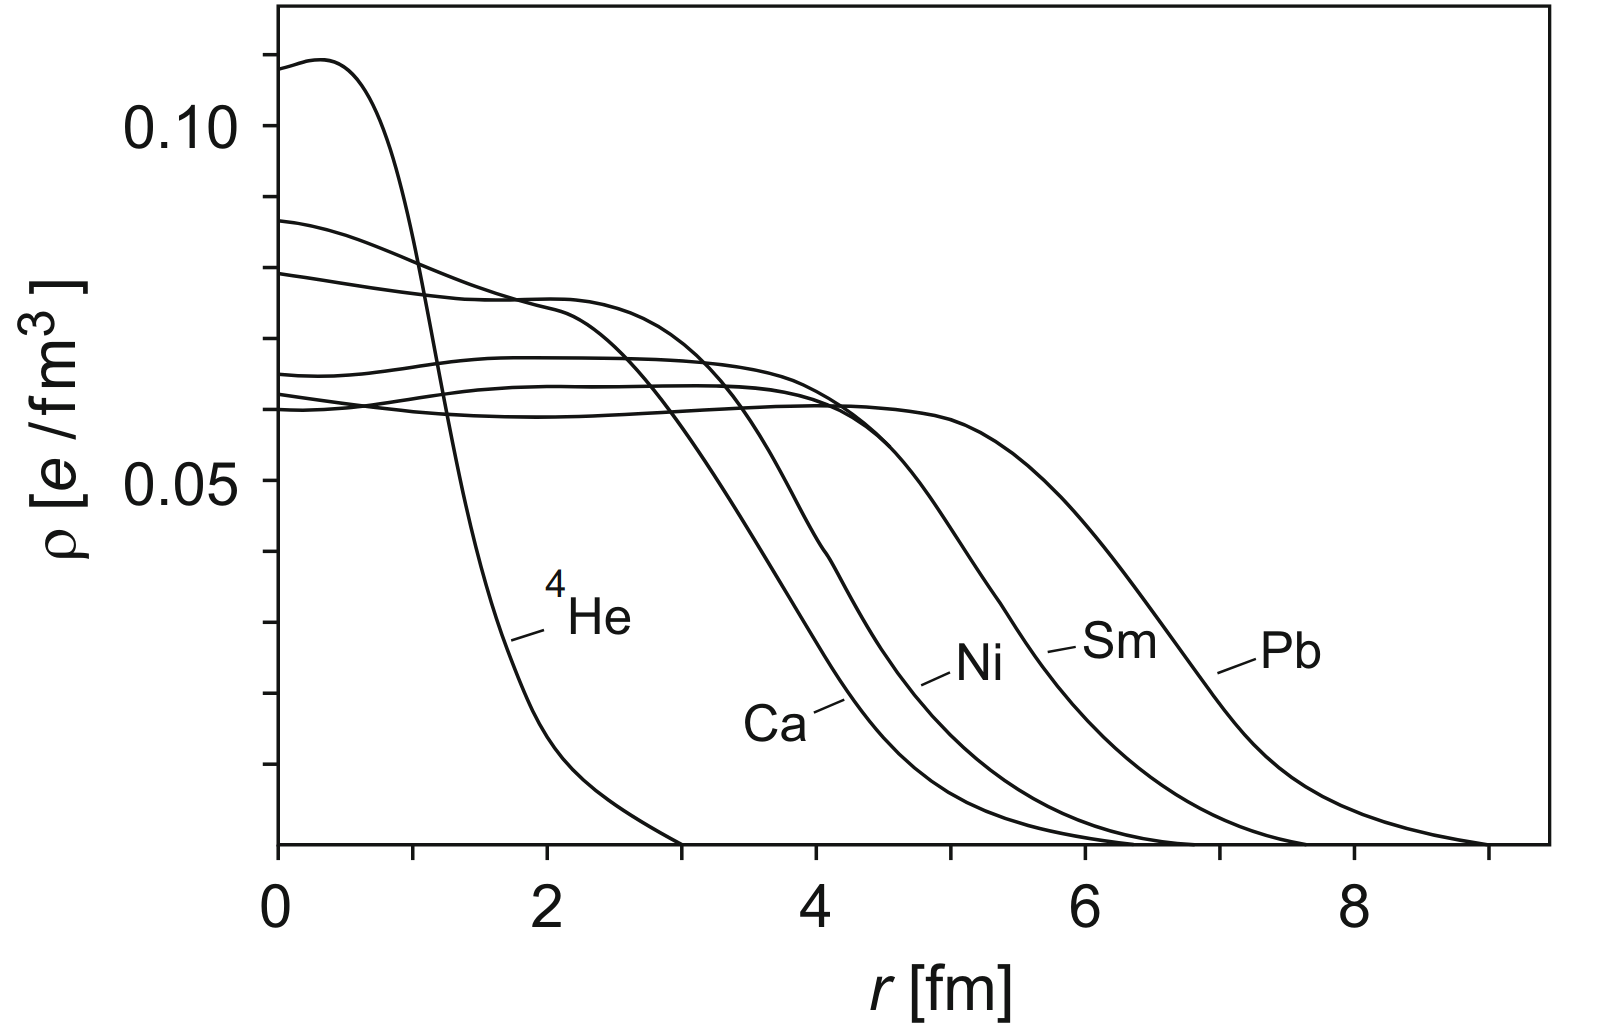
\includegraphics[width=0.95\textwidth]{charge-distribution.png}
	\caption{Distribuzione di carica in vari nuclidi.}
	\label{charge-distr}
\end{figure}

Sperimentalmente si trova che alcuni nuclidi (ad esempio i lantanidi) non hanno una forma sferica ma assumono deformazioni ellissoidali: queste forme non possono essere studiate con scattering elettronico, poiché esso evidenzia soltanto una superficie molto diffusa.\\
Va infine notato che nuclidi leggeri come $ \ch{^{6,7}Li} $, $ \ch{^{9}Be} $ e soprattutto $ \ch{^{4}He} $ costituiscono dei casi speciali: essi non presentano una densità di carica centrale costante, ma il suo andamento è approssimativamente gaussiano.

\subsubsection{Nuclidi instabili}

Quanto riportato fin'ora vale solo per nuclidi nella valle di stabilità (vedere Fig. \ref{segre-chart}), ovverosia l'insieme di nuclei stabili che non decadono radioattivamente (tipicamente per decadimento $ \beta $), i quali sono osservati in abbondanza sulla Terra.\\
Se, partendo dalla valle di stabilità, si percorre una catena isotopica, i nuclidi diventano via via più neutron-rich, fino a quando non si raggiungono le driplines, oltre le quali i nuclei non sono più sistemi legati a causa dell'interazione nucleare forte.\\
Lo spostamento verso nuclidi esotici neutron-rich causa un mutamento drastico rispetto ai loro isotopi stabili: in un lavoro pionieristico del 1985 di Tanihata et al., fu misurata la cross-section d'interazione tra nuclei di $ \ch{^{11}Li} $ (isotopo instabile) e dei nuclidi stabili target, la quale può essere teoricamente calcolata dal modello di Glauber per lo scattering relativistico di nuclidi (traiettorie iniziali e finali rettilinee) come $ \sigma_I \sim \pi \left( R_p^2 + R_t^2 \right) $, dove $ R_p $ è il raggio del nucleo proiettile ed $ R_t $ quello del nucleo target; dai dati fu possibile ricavare il raggio nucleare del $ \ch{^{11}Li} $, il quale dovrebbe essere dell'ordine di $ \sim 2.4\fm $, trovando un valore cinque volte maggiore (comparabile con quello del $ \ch{^{208}Pb} $): questa fu la prima verifica sperimentale dell'esistenza di sistemi ad alone, nuclidi con un corpo centrale sferico circondati da uno o due neutroni o protoni (si parla di neutron skin o proton skin), i quali vanno a formare un halo attorno al nucleo aumentandone considerevolmente le dimensioni osservate.\\
Condurre esperimenti di scattering elettronico su nuclei instabili è estremamente difficile, poiché pochi di essi hanno delle vite medie abbastanza lunghe, dunque non è possibile predisporre un target composto del materiale da studiare: in alcuni laboratori si è riusciti a costruire delle trappole con le quali i nuclidi instabili sono accellerati e confinati, così da poter essere bombardati da fasci elettronici.

\paragraph{Luminosità}

Nello studio dei rilevatori di scattering un importante parametro è la luminosità:
\begin{equation}
	\mathcal{L} = N_b N_t
	\label{eq:15}
\end{equation}
dove $ N_b $ è il numero di particelle incidenti per unità di tempo e $ N_t $ il numero di nuclidi target per unità d'area.\\
Questo parametro è legato all'efficienza del rilevatore, misurata dal numero di eventi rilevati nell'unità di tempo $ \dot{N} $:
\begin{equation}
	\dot{N} (E, \theta) = \mathcal{L}\, \frac{d\sigma}{d\Omega} (E,\theta) \,\Delta\Omega
	\label{eq:16}
\end{equation}
Nel caso dello scattering elettronico, la cross-section è molto piccola, dunque sono necessari collisori dall'elevata luminosità (tecnicamente difficile): si va da $ \mathcal{L}_{\text{min}} \sim 10^{26} \,\text{cm}^{-2} \,\text{s}^{-1} $ per sondare nuclidi con $ Z \sim 80 $ a $ \mathcal{L}_{\text{min}} \sim 10^{31} \,\text{cm}^{-2}\,\text{s}^{-1} $ per $ Z \sim 10 $.\\
Inoltre, la luminosità varia anche in base al target considerato: per nuclidi stabili si raggiungono luminosità per scattering elettronico di $ 10^{33} \,\text{cm}^{-2}\,\text{s}^{-1} $ (es: STABLE), mentre su nuclidi instabili si arriva a $ 10^{27} \,\text{cm}^{-2}\,\text{s}^{-1} $ (es: SCRIT).

\section{Proprietà dei nuclidi}

\subsection{Masse nucleari}

Preso un atomo di una specie chimica $ ^A_Z \text{X}_N $, se si sommano le masse degli $ N $ neutroni, dei $ Z $ protoni e dei $ Z $ elettroni, si trova una massa minore di quella misurata per l'atomo: questo avviene poiché, essendo l'atomo uno stato legato, parte della massa dei suoi costituenti viene convertita in energia di legame (positiva, poiché stato legato), ovvero:
\begin{equation}
	M_{\text{atom}} = N m_n + Z \left( m_p + m_e \right) - \frac{1}{c^2} \left( B_{\text{atom}} + B_{\text{nucleus}} \right)
	\label{eq:1.17}
\end{equation}
dove si è distinto tra binding energy atomica e nucleare: queste ultime sono conosciute con incertezze maggiori, dato che $ (\delta m / m)_{\text{atom}} \sim 10^{-10} $ e $ (\delta m / m)_{\text{nucleus}} \sim 10^{-7} $.\\
Si trova quindi che la binding energy di un nuclide può essere espressa come:
\begin{equation}
	B(A,Z) = \left[ Z m({\ch{^{1}H}}) + N m_n - M(A,Z) \right] c^2
	\label{eq:1.18}
\end{equation}
dove si sono usate le masse atomiche, poiché misurate con più precisione (si ricordi la conversione $ 1u \approx 931.494\mev/c^2 $).\\
La misura delle masse atomiche è importante poiché permette di fare misure indirette sulle masse nucleari, e dunque studiare l'abbondanza isotopica di un elemento, e di stimare le binding energies, le quali sono legate alla natura della forza nucleare.\\
Ci sono varie tecniche per misurare le masse atomiche: spettrometri di massa, cinematica delle reazioni (solitamente quando i primi non si possono utilizzare), trappole (ad oggi gli strumenti più precisi) ed anelli di accumulazione (storage rings).

\subsubsection{Spettrometri di massa}

Uno spettrometro di massa permette di misurare le masse di ioni di un determinato elemento.
\begin{figure}[!b]
	\centering
	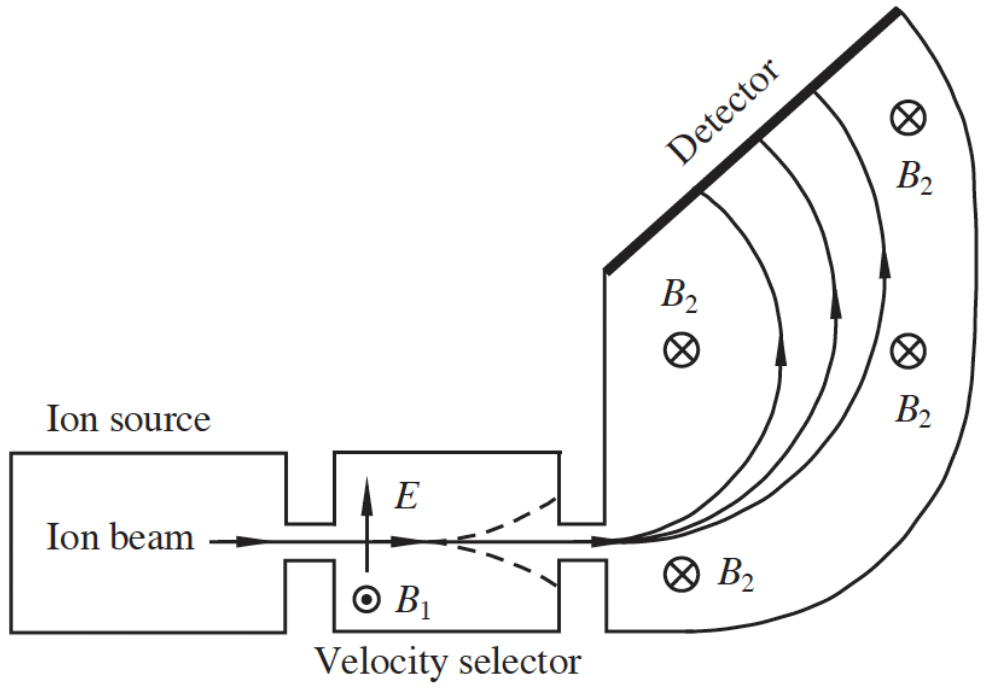
\includegraphics[width=0.75\textwidth]{spectrometer.png}
	\caption{Schematizzazione di uno spettrometro di massa.}
	\label{spettr}
\end{figure}

Schematicamente (Fig. \ref{spettr}), esso è costituito da:
\begin{itemize}
	\item una sorgente di ioni;
	\item un selettore di velocità;
	\item uno spettrometro magnetico;
	\item un focal plane detector.
\end{itemize}
La sorgente di ioni ionizza gli atomi da studiare, li accellera e li collima in un fascio; questo fascio viene diretto in un selettore di velocità: questo è solitamente un filtro di Wien, composto da un campo elettrico e un campo magnetico incrociati che determinano traiettorie rettilinee solo se $ \ve{F}_E + \ve{F}_B = \ve{0} $, ovvero, assumendo un fascio già collimato nella direzione desiderata, se $ v = E / B $.\\
L'elemento ottico di questo setup è lo spettrometro magnetico: in esso le traiettorie degli ioni curvano in base al loro momento e alla loro carica, dato che il raggio di girazione è $ r = \frac{vm}{qB} $: di conseguenza, sperimentalmente vanno misurati sia il raggio di girazione che la carica per poter determinare la massa dello ione, e ciò è proprio quello che fa il focal plane detector.\\
Va notato che, in generale, le misure assolute di massa non permettono una grande precisione, perciò si preferisce effettuare misurazioni rispetto a ioni di cui già di conosce bene la massa: in particolare, le precisioni maggiori si raggiungono sui mass ratios tra ioni di egual carica, poiché in tal caso $ m_1 / m_2 = r_1 / r_2 $. Il campione di riferimento solitamente utilizzato è il carbonio, poiché dati i suoi numerosi composti permette di effettuare misure su un vasto range di ioni.

\paragraph{Abbondanze isotopiche}

Tendenzialmente, un elemento avrà più di un isotopo stabile (if any at all), dunque con una spettrografia di massa risulterà una distribuzione di massa con picchi di abbondanza relativa corrispondenti agli isotopi stabili: ciò permette di misurarne le masse $ m_i $ e l'abbondanza percentuale nel campione $ w_i $, così da poter stimare la massa atomica dell'elemento come media ponderata $ m = \sum_{i} w_i m_i $.\\
In generale, le abbondanze isotopiche sono diverse nell'Universo rispetto alla Terra, ed anche sulla Terra possono avere forti fluttuazioni tra una zona geografica e l'altra; ad esempio, si considerino due campioni di $ \ch{Xe} $, uno prelevato da una roccia metamorfica vecchia di $ 2.7 \text{Gy} $ ed uno dall'atmosfera: le relative analisi spettrografiche (riportate in Fig. \ref{iso-distr}) mostrano delle diverse abbondanze isotopiche nei due campioni, dovute alla presenza nella roccia metamorfica di prodotti della fissione nucleare spontanea dell'uranio.
\begin{figure}[!b]
	\centering
	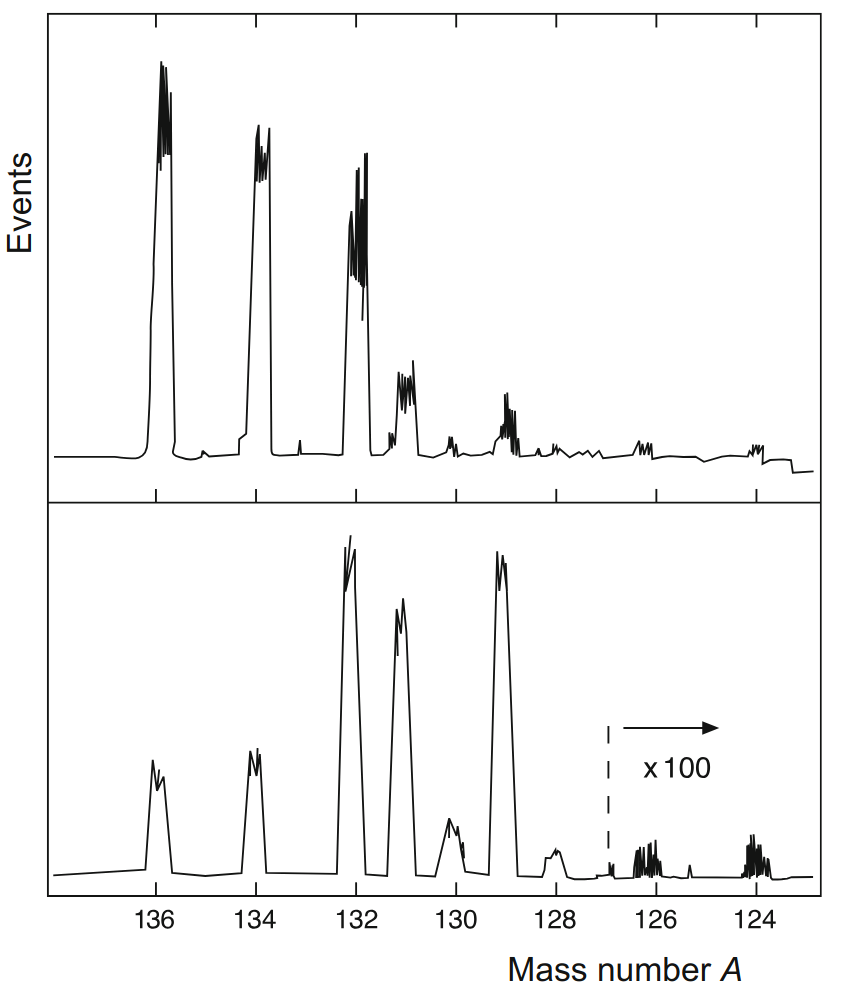
\includegraphics[width=0.55\textwidth]{isotop-distr.png}
	\caption{Distribuzioni isotopiche di due campioni di $ \ch{Xe} $, il primo prelevato da una roccia metamorfica, il secondo dall'atmosfera.}
	\label{iso-distr}
\end{figure}

\begin{figure}[!ht]
	\centering
	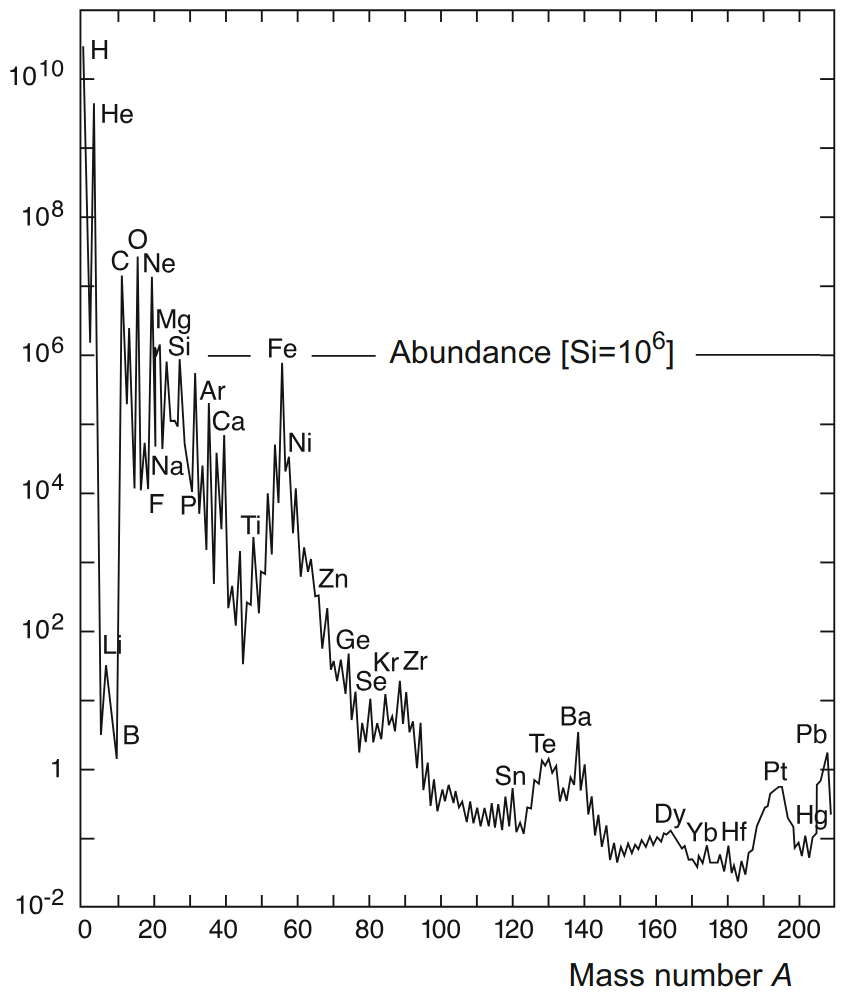
\includegraphics[width=0.75\textwidth]{isotop-distr-univ.png}
	\caption{Distribuzioni isotopiche dei principali elementi nel Sistema Solare, normalizzati all'abbondanza del $ \ch{Si} $: l'abbondanza del $ \ch{Li} $ è uno dei problemi nella ricostruzione dell'origine dell'Universo.}
	\label{iso-distr-univ}
\end{figure}
Lo studio delle abbondanze relative nell'Universo (Fig. \ref{iso-distr-univ}) permette di studiarne l'evoluzione: secondo gli attuali modelli, la sintesi di deuterio ed elio è avvenuta all'origine dell'Universo dalla fusione nucleare dell'idrogeno, mentre i nuclidi fino al $ \ch{^{56}Fe} $ vengono sintetizzati dalla fusione nucleare nei nuclei stellari; per quanto riguarda i nuclei pesanti, invece, la loro sintesi avviene nelle esplosioni di stelle molto massive.

\subsubsection{Cinematica delle reazioni}

Qualora il tempo di volo tra il generatore di ioni ed il piano focale fosse maggiore della vita media dello ione che si vuole studiare, al posto della spettroscopia di massa è possibile calcolare la massa dello ione studiandone le sue reazioni.\\
Si consideri una reazione del tipo:
\begin{equation}
	a + \text{X} \longrightarrow b
	\label{eq:1.19}
\end{equation}
dove $ a $ è la particella proiettile, $ \text{X} $ lo ione target e $ b $ rappresenta l'insieme di prodotti della reazione.\\
Assumendo uno scattering elastico, la conservazione dell'energia ci dà:
\begin{equation}
	m_a c^2 + T_a + m_{\text{X}} c^2 + T_{\text{X}} = m_b c^2 + T_b
	\label{eq:1.20}
\end{equation}
È possibile definire il cosiddetto Q-value della reazione:
\begin{equation}
	Q \defeq T_{\text{final}} - T_{\text{initial}} = T_b - T_a - T_{\text{X}}
	\label{eq:1.21}
\end{equation}
così da poter calcolare la massa dell'isotopo $ \text{X} $ come:
\begin{equation}
	m_{\text{X}} = \frac{1}{c^2} Q + m_b - m_a
	\label{eq:1.22}
\end{equation}
Con questo metodo, è possibile raggiungere una precisione $ \delta m / m \sim 10^{-6} $.

\subsubsection{Trappole}

Le trappole sono dispositivi in grado di confinare ioni grazie a campi elettromagnetici finemente controllati. Esse vengono usate soprattutto quando la vita media dello ione radioattive non permette l'utilizzo né di spettrometri di massa (a causa del tempo di volo) né di reazioni cinematiche (per sezioni d'urto bassissime).\\
Il vantaggio delle trappole è che permettono lo studio prolungato anche di singoli radioisotopi in regimi energetici bassissimi, dunque con velocità pressoché nulle, limitatamente alle loro vite medie.\\
Sebbene le trappole abbiano incertezze relative bassissime ($ \delta m / m \sim 10^{-8} $ per nuclidi instabili e $ 10^{-11} $ per nuclidi stabili), in determinati si sceglie di usare gli anelli di accumulazione poiché, nonostante le incertezze leggermente più alte, permettono di raggiungere energie relativistiche, rendendo possibili misurazioni su isotopi con vite medie cortissime.

\paragraph{Trappola di Penning}

Una trappola costituita da 4 elettrodi pensata per isotopi prodotti con velocità basse (principalmente tecnica ISOL\footnote{Ioni incidono su una lastra di carbonato di uranio a $ 4000\cels$ così da poter effondere e diffondere attraverso la superficie con un'energia cinetica bassissima; sono possibili anche tecniche di accellerazione e post-accellerazione.}), i quali vengono confinati radialmente da un campo magnetico (per moto di ciclotrone) ed assialmente da un campo elettrostatico di quadrupolo.\\
Il moto all'interno della trappola è molto complicato, poiché somma di un moto di magnetone circolare attorno all'asse di $ \ve{B} $ con frequenza $ \omega_- $, un moto di ciclotrone spiraleggiante attorno alle linee di $ \ve{B} $ con frequenza $ \omega_+ $ ed un moto oscillatorio longitudinale determinato da $ \ve{E}_{\text{quad}} $ con frequenza $ \omega_z $. Si dimostra il seguente teorema d'invarianza:
\begin{equation}
	\omega_c^2 = \omega_+^2 + \omega_-^2 + \omega_z^2
	\label{eq:1.23}
\end{equation}
Ciò permette di misurare la massa dello ione, ricordando che la frequenza di ciclotrone è $ \omega_c = \frac{q B}{m} $.\\
Le misure effettuate sono sempre misurazioni relative di massa (solitamente con campione $ \ch{^{12}C} $), così da includere eventuali errori sistematici.

\subsubsection{Anelli di accumulazione}

Un anello di accumulazione è un accelleratore di particelle circolare in cui un fascio di ioni viene fatto circolare a velocità relativistica per un periodo prolungato di tempo.\\
Gli ioni vengono prodotti con velocità relativistiche (principalmente tecnica in flight\footnote{Nuclei radioattivi (es: $ \ch{^{238}U} $) vengono accellerati a diverse centinaia di MeV per nucleone e fatti scontrare su target di $ \ch{^{9}Be} $, frammentandosi in prodotti con velocità relativistiche, i quali vengono poi selezionati da strumenti ottici in base al rapporto $ m/q $.}) ed immessi nell'anello; la loro massa è determinata dal periodo di rivoluzione:
\begin{equation}
	\frac{\Delta T}{T} = \frac{1}{\gamma_t^2}\frac{\Delta (m/q)}{m/q} - \left( 1 - \frac{\gamma^2}{\gamma_t^2} \right) \frac{\Delta v}{v}
	\label{eq:1.24}
\end{equation}
Il secondo termine è una correzione dovuta alla transition energy (il valore per cui l'energia diventa indipendente dalla specie chimica nell'anello) e alla dispersione delle velocità, ed è eliminabile tramite tecniche ingegneristiche: in particolare, esistono anelli di accumulazione progettati col metodo di Schottky (cool fragments), per i quali $ \frac{\Delta v}{v} \rightarrow 0 $, e quelli a traiettorie isocrone (hot fragments, così da avere energia pari all'energia di transizione), per i quali $ \gamma_t \rightarrow \gamma $. Con questi anelli di accumulazione si raggiunge $ \delta m / m \sim 10^{-8} $.

\subsection{Binding energy}

Riprendendo l'Eq. \ref{eq:1.18}, si definisce la binding energy di un nuclide $ ^A_Z \text{X}_N $ come:
\begin{equation}
	B(A,Z) = \left[ Z m({\ch{^{1}H}}) + N m_n - M(A,Z) \right] c^2
	\label{eq:1.25}
\end{equation}
La binding energy è positiva nel caso di nuclidi legati, ovvero quelli che possono effettivamente esistere nel loro stato fondamentale (anche se con vite medie corte).\\
Come si può vedere in Fig. \ref{bind-en}, se si restringe l'analisi ai nuclidi stabili e long-lived, si nota che, a seguito di rapide variazioni per bassi $ A $, la binding energy per nucleone si stabilizza a circa $ 8\mev/\text{nucleone} $ per i pesanti (oltre il $ \ch{^{56}Fe} $): i nuclei più stabili sono $ \ch{^{62}_{28}Ni} $, $ \ch{^{58}_{26}Fe} $ e $ \ch{^{56}_{26}Fe} $.
\begin{figure}[!ht]
	\centering
	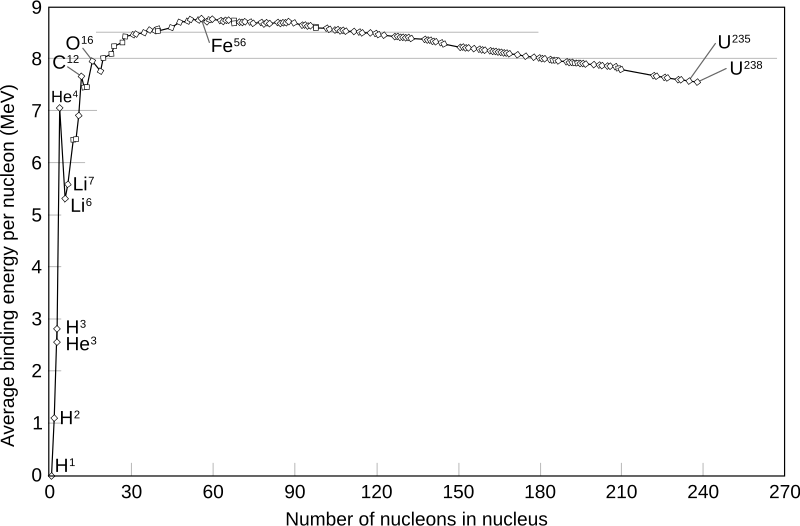
\includegraphics[width=0.75\textwidth]{bind-en.png}
	\caption{Binding energy table for stable and long-lived nuclei.}
	\label{bind-en}
\end{figure}

Sempre dal grafico in Fig. $ \ref{bind-en} $ è possibile fare alcune considerazioni:
\begin{enumerate}
	\item i nuclei pari-pari (numero pari di neutroni e di protoni) sono energeticamente favoriti rispetto a quelli pari-dispari, poiché più legati (es: $ \ch{^{4}He} $ è il nuclide leggero più legato), inoltre non ci sono nuclidi stabili per $ A = 5,8 $;
	\item il rapporto $ B/A \sim 8\mev $ costante per i nuclei pesanti evidenzia la natura a corto raggio dell'interazione forte, la quale viene saturata (un nucleone risente solo dei nucleoni vicini);
	\item il picco attorno ad $ A \sim 60 $ mostra come, tendendo all'equilibrio, i nuclidi leggeri guadagnano energia formando nuclei più pesanti tramite fusione nucleare (es: ambiente stellare), mentre i nuclidi pesanti perdono energia separandosi in nuclei leggeri tramite fissione nucleare.
\end{enumerate}
È necessario fare una precisazione: un nuclide può essere legato ma comunque instabile. Ad esempio, il $ \ch{^8 Be} $ ha $ B = 56.5\mev $, ma rispetto al decadimento $ \alpha $ si ha $ \ch{^8 Be} \rightarrow 2\alpha $, il quale ha una variazione d'energia $ B_{\text{decay}} = - 0.092\mev $: si evince che nel suo stato fondamentale il $ \ch{^8 Be} $ non esiste in uno stato legato, ma come risonanza di due particelle $ \alpha $, la quale sussiste per un certo periodo di tempo prima di decadere.\\
In generale, se esiste almeno una combinazione di neutroni e protoni non legata, allora il nuclide allo stato fondamentale non esiste in uno stato legato e decade; inoltre, di solito sono possibili varie modalità di decadimento, dette decay branches.

\subsubsection{Formula semi-empirica di Weizsäcker}

È possibile dare un'interpretazione fenomenologica della binding energy tramite un modello semplificato del nucleo atomico: il modello a goccia. Questo modello si basa sulle seguenti ipotesi:
\begin{enumerate}
	\item l'energia d'interazione tra due nucleoni è indipendente dal tipo e dal numero di nucleoni (non si distingue tra neutroni e protoni);
	\item l'interazione tra nucleoni è attrattiva a breve raggio per $ r < R_{\text{int}} $ e repulsiva a brevissimo raggio per $ r \ll R_{\text{int}} $;
	\item la binding energy del nucleo è proporzionale al numero di nucleoni (e dunque al volume del nucleo).
\end{enumerate}
Questo modello implica delle forze sature tra nucleoni, in cui ciascuno nucleone è legato solo ai nucleoni immediatamente vicini; definendo l'energia d'interazione tra due nucleoni $ \langle U \rangle $, ciò implica che la binding energy del nucleo non è data dalla somma di tutte le coppie di nucleoni, ma solo delle coppie vicine in un volume $ V_{\text{int}} < V_{\text{nucleo}} $. Ricordando che $ V_{\text{nucleo}} \sim A $, si ha:
\begin{equation}
	B_0 = \sum_{r < R_{\text{int}}} U = \frac{A(A-1)}{2}\langle U \rangle \frac{V_{\text{int}}}{V_{\text{nucleo}}} \sim b_0 A
	\label{eq:1.26}
\end{equation}
A questa stima cruda vanno aggiunti dei termini correttivi per effetti di cui il modello a goccia non tiene conto.\\
Innanzitutto, va considerato un termine di superficie, dovuto al fatto che i nucleoni sulla superficie del nucleo interagiscono con un minor numero di nucleoni, dunque sono meno legati; dato che il raggio atomico è $ R \sim A^{1/3} $, il termine di superficie va come $ B_{\text{sup}} \sim - b_1 A^{2/3} $.\\
Bisogna anche considerare la repulsione coulombiana tra protoni, la quale può essere approssimata col modello della sfera uniformemente carica (dai form factors, $ \rho $ è circa costante all'interno del nucleo):
\begin{equation}
	 U_e = \int_0^R V(r) \rho(r) 4\pi r^2 dr = \int_0^R \frac{Ze}{4\pi \epsilon_0 r} \left( \frac{r}{R} \right)^3 \frac{Ze}{\frac{4}{3}\pi R^3} 4\pi r^2 dr = \frac{3}{5} \frac{(Ze)^2}{4\pi \epsilon_0 R}
	\label{eq:1.27}
\end{equation}
Dunque va aggiunta una correzione $ B_{\text{Coulomb}} \sim - b_2 \frac{Z^2}{A^{1/3}} $.\\
Essendo il nucleo un sistema quantistico, è naturale che nella sua descrizioni siano inclusi gli effetti quantistici: in particolare, il calcolo dell'energia cinetica dei nucleoni può essere svolto prendendo come modello un gas di Fermi, il quale tiene conto della statistica dei fermioni e del principio di esclusione di Pauli (questo favorisce la formazione di nuclei con egual numero di protoni e neutroni); l'energia cinetica totale risulta essere:
\begin{equation}
	K_{\text{tot}} \approx 20 \mev \left( A + \frac{5}{9} \frac{(N - Z)^2}{A} \right)
	\label{eq:1.28}
\end{equation}
Il primo termine si aggiunge al termine di volume $ B_0 $, mentre il secondo termine determina un termine correttivo $ B_{\text{sym}} \sim - b_3 \frac{(N - Z)^2}{A} $.\\
Infine, lo studio delle masse nucleari mostra che i nuclei con un numero pari di protoni e/o neutroni sono più stabili: ciò viene interpretato come un accoppiamento a doppietti sia dei protoni che dei neutroni (in base ai loro spin e momento angolare, in modo da avere spin totale nullo). Empiricamente, ciò determina un fattore correttivo alla binding energy pari a:
\begin{equation}
	B_{\text{parity}} \sim - \delta A^{-1/2}, \qquad \delta =
	\begin{cases}
		+11.2\mev & \text{dispari-dispari} \\
		0\mev & \text{dispari-pari o pari-dispari} \\
		-11.2\mev & \text{pari-pari}
	\end{cases}
	\label{eq:1.29}
\end{equation}
Si è sostanzialmente ricavata la \textit{formula semi-empirica di Weizsäcker}:
\begin{equation}
	B(A,Z) = a_V A - a_S A^{2/3} - a_C \frac{Z^2}{A^{1/3}} - a_a \frac{(N - Z)^2}{A} - \delta A^{-1/2}
	\label{eq:1.30}
\end{equation}
dove $ \delta $ è definito in Eq. $ \ref{eq:1.29} $ e gli altri parametri fenomenologici si trovano essere $ a_V = 15.835\mev $, $ a_S = 18.33\mev $, $ a_C = 0.714\mev $ e $ a_a = 23.20\mev $.\\
Lungo le catene isotopiche ($ A = $ const.) $ B(Z) $ è una parabola: è possibile trovare $ Z_{\text{min}} $ analiticamente, ottenendo che per $ A $ grande è $ Z_{\text{min}} < \frac{A}{2} $, mentre per $ A $ piccolo $ Z_{\text{min}} \approx \frac{A}{2} $, e questa condizione dà il nuclide più stabile della catena isotopica considerata. Nel caso di catene con $ A $ pari, si ha una doppia parabola a causa del termina di pairing $ \delta $ (vedere Fig. \ref{iso-chain}).
\begin{figure}[!h]
	\centering
	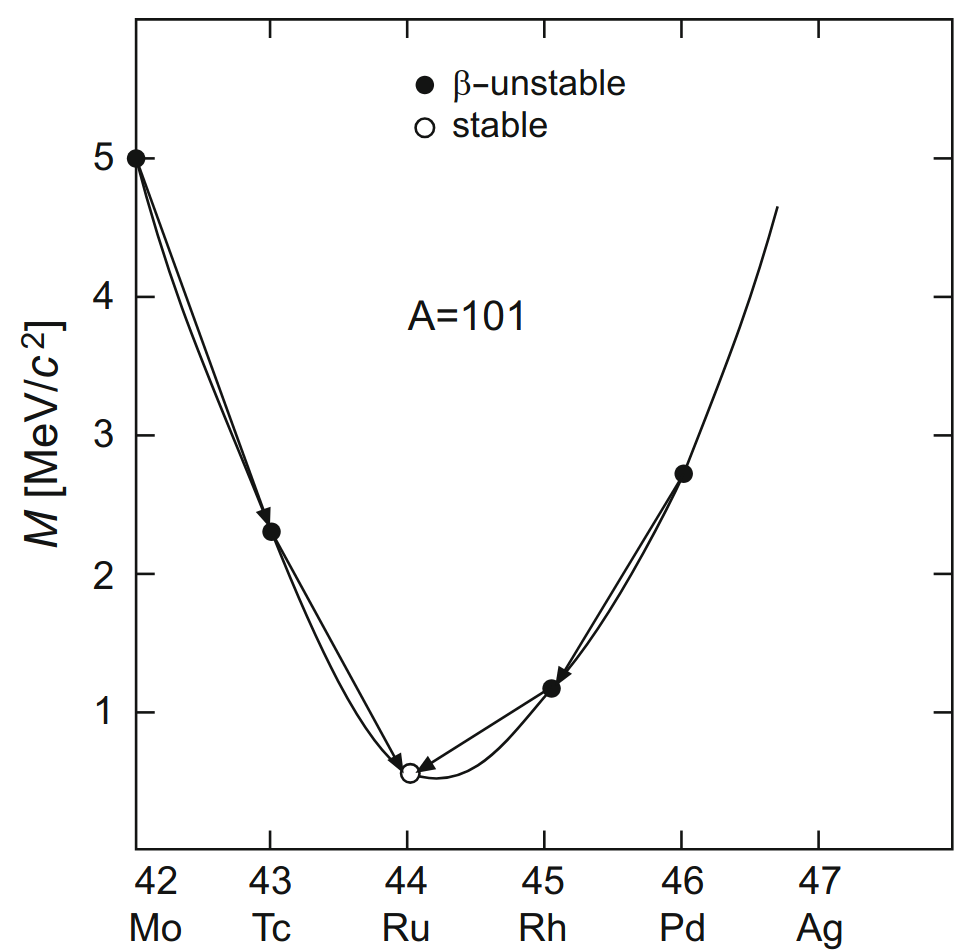
\includegraphics[width=0.45\textwidth]{iso-chain-odd.png}
	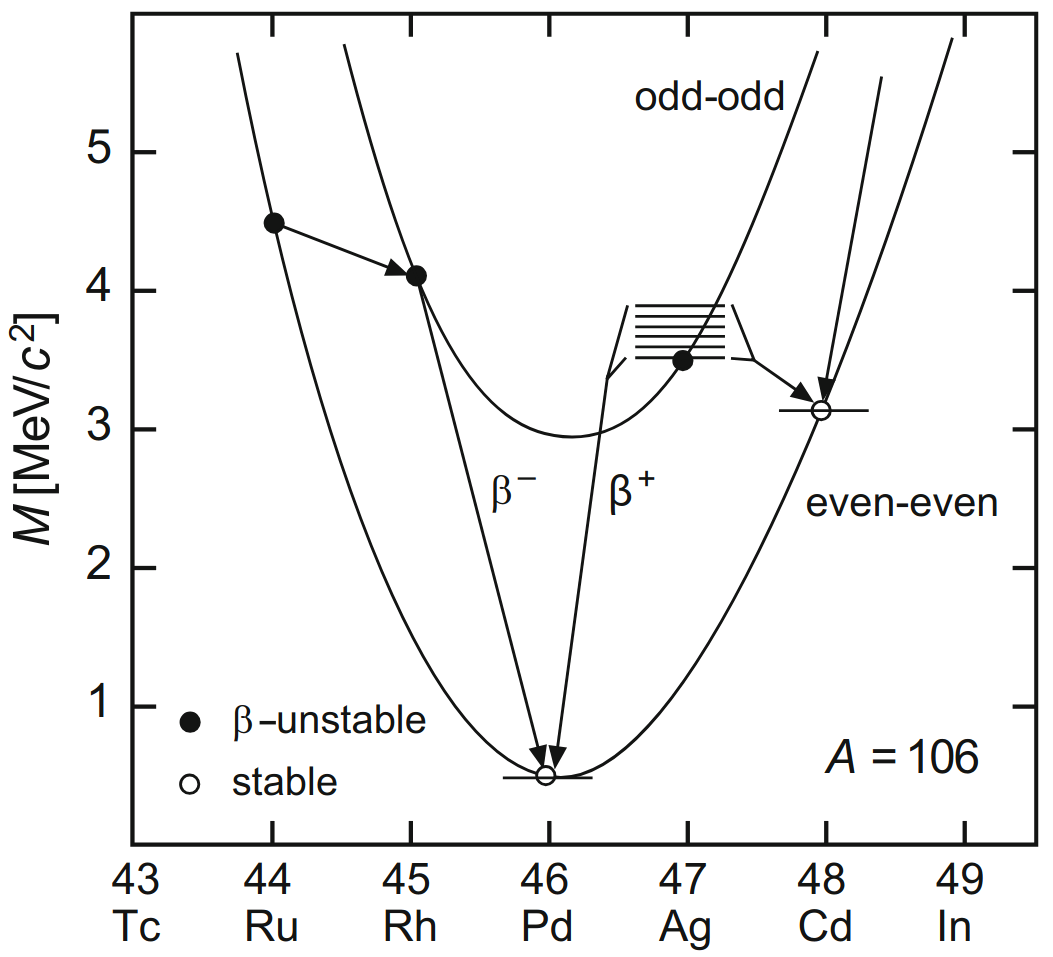
\includegraphics[width=0.45\textwidth]{iso-chain-even.png}
	\caption{Isotopic chain with $ A = 101 $ and $ A = 106 $.}
	\label{iso-chain}
\end{figure}

Tendenzialmente, i nuclidi instabili si riconducono alla stabilità tramite decadimento $ \beta $, sia $ p^+ \rightarrow n $ che $ n \rightarrow p^+ $. In casi particolari, alcuni nuclidi con $ N $ e $ Z $ dispari possono decadere con un doppio decadimento $ \beta $.\\
La formula semi-empirica ha un ottimo accordo coi dati sperimentali per i nuclei pesanti, con errori di circa $ \pm 1\% $, mentre per i nuclei leggeri sono presenti alcune discrepanze: a basso $ A $, il modello a goccia diventa poco accurato.\\
Inoltre, va notato che il modello presenta delle grosse incertezze (sia per le masse che per le abbondanze isotopiche) per isotopi senza valori sperimentali delle masse.

\subsection{Momento angolare e spin}

Gli elettroni negli atomi si dispongono su orbite quantizzate dai numeri quantici dell'elettrone:
\begin{itemize}
	\item numero quantico principale $ n \in \N $, determina il livello energetico dell'elettrone;
	\item numero quantico orbitale $ \ell \in \left[ 0, n-1 \right] \subset \N $, determina il momento angolare orbitale dell'elettrone;
	\item numero quantico magnetico $ m \in \left[ -\ell, \ell \right] \subset \N $, legato alla proiezione del momento angolare sull'asse $ z $ (convenzione);
	\item numero quantico di spin $ s = \pm \frac{1}{2} $, determinante lo spin dell'elettrone.
\end{itemize}
Si ricordi che lo spin, sebbene rappresentato come una rotazione su sé stesso dell'elettrone, è un concetto puramente quanto-meccanico introdotto da Dirac: l'elettrone è privo di struttura interna, quindi non può ruotare su sé stesso.\\
Data la dualità onda-particella, gli elettroni non sono localizzati nello spazio, ma sono caratterizzati da distribuzioni di probabilità che determinano la probabilità d'interazione di un elettrone in un singolo punto: queste distribuzioni sono determinate dalla funzione d'onda dell'elettrone, la quale è ricavata risolvendo l'equazione di Schrödinger per l'atomo considerato, ed in particolare si ha $ P(x) = \abs{\psi(\ve{x})}^2 $.\\
Per l'atomo più semplice, $ \ch{^1 H} $, si trova:
\begin{equation}
	\psi(r,\theta,\phi) = R_{n,\ell,m}(r) Y_{\ell}^m(\theta,\phi)
	\label{eq:1.31}
\end{equation}
dove $ R_{n,\ell,m}(r) $ è la parte radiale della soluzione e $ Y_{\ell}^m(\theta,\phi) $ quella angolare, data dalle armoniche sferiche:
\begin{equation}
	Y_{\ell}^m(\theta,\phi) = \sqrt{\frac{(2\ell+1)(\ell-m)!}{4\pi(\ell+m)!}} e^{im\phi} P_{\ell}^m(\cos\theta)
	\label{eq:1.32}
\end{equation}
Le deistribuzioni di probabilità per i primi orbitali dell'atomo di $ \ch{^1 H} $ sono plottate in Fig. \ref{hyd-pd}.
\begin{figure}
	\centering
	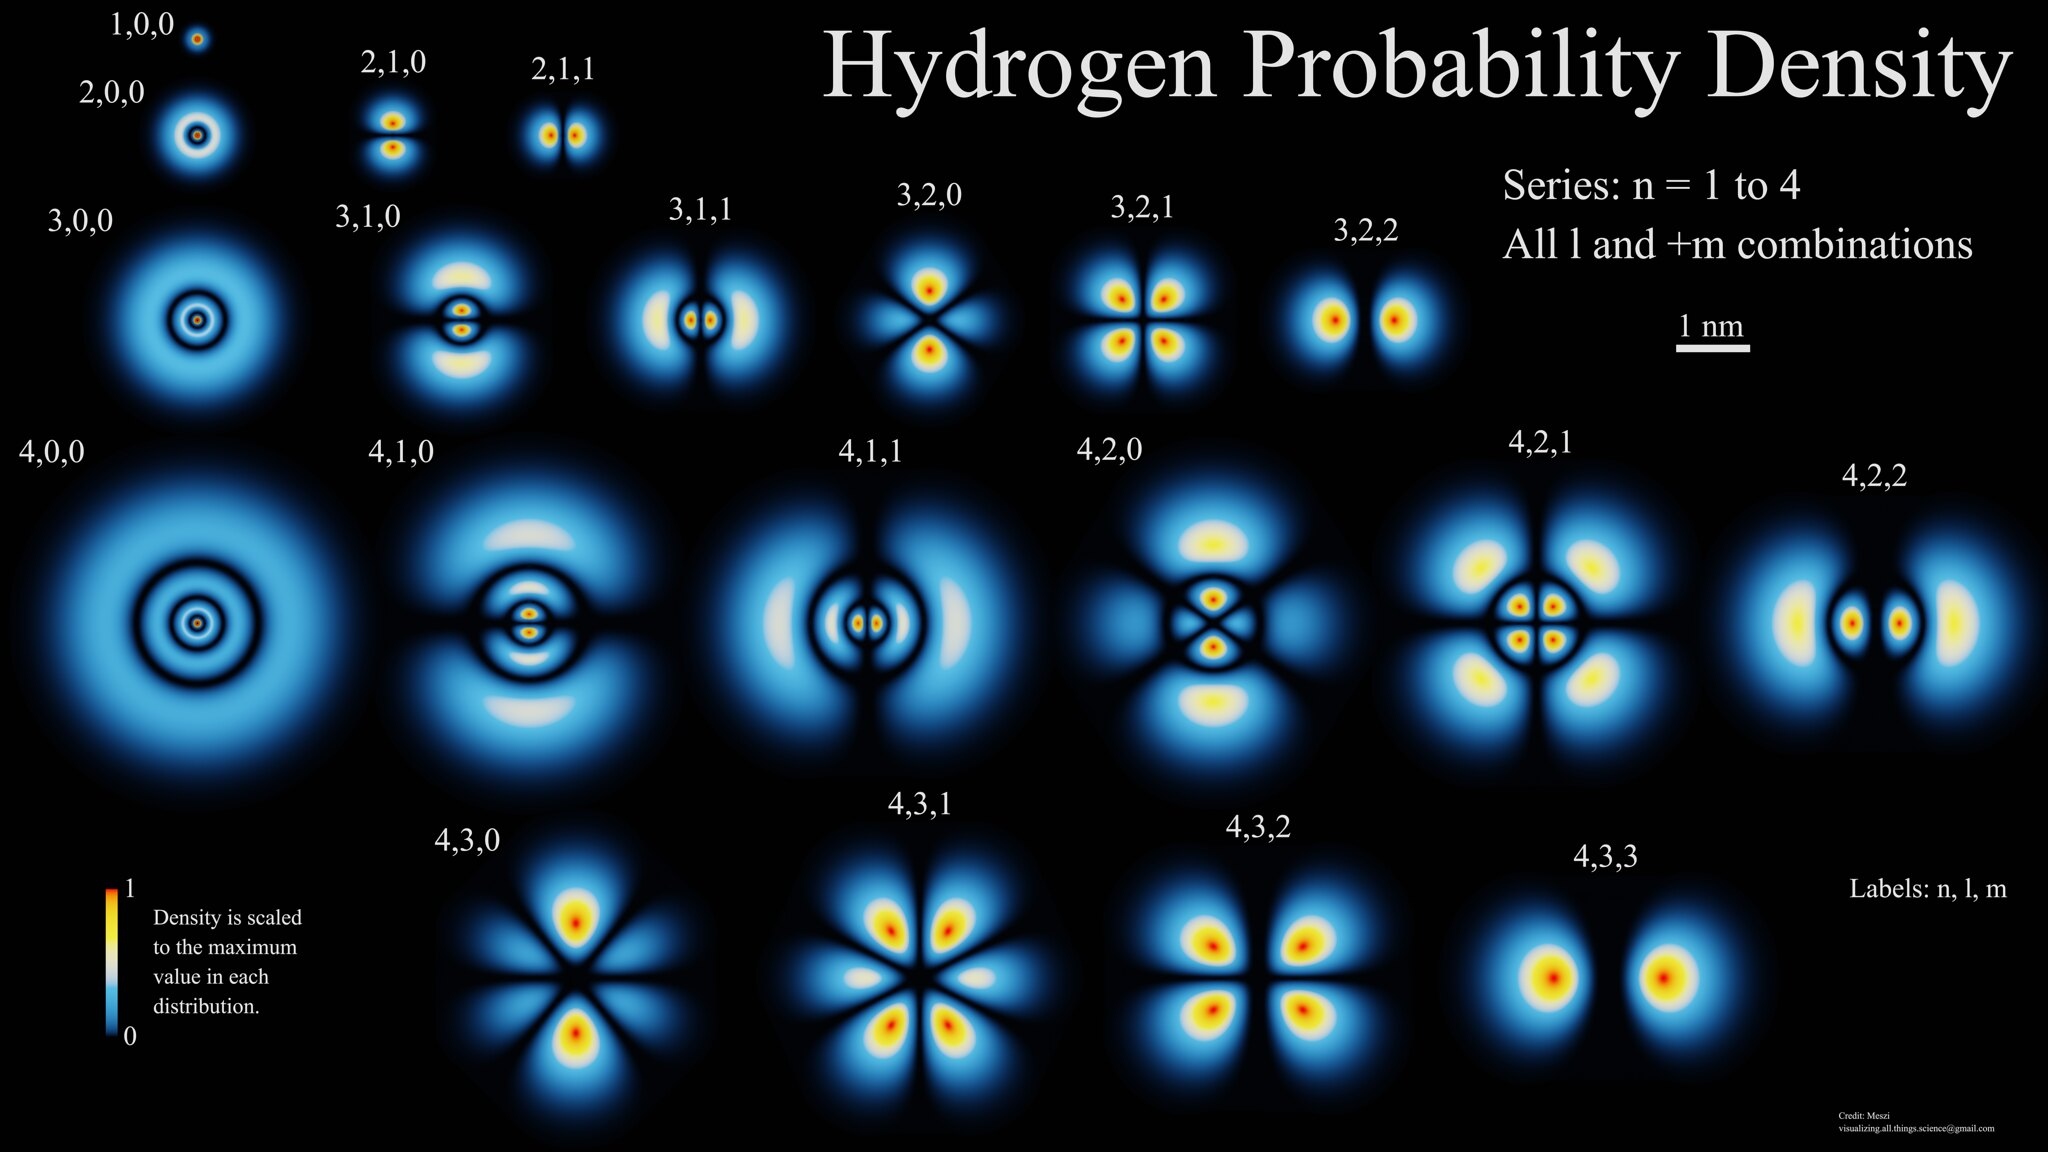
\includegraphics[width=\textwidth]{hydrogen-pd.png}
	\caption{Probability distributions for $ \ch{^1 H} $ atom.}
	\label{hyd-pd}
\end{figure}

Lo stesso modello adottato per gli elettroni è stato adottato anche per quanto riguarda protoni e neutroni nel nucleo: in questo caso, essendo i nucleoni dotati di struttura interna, ha senso immaginare lo spin come il momento angolare associato ad una rotazione del nucleone su sé stesso, basti ricordare che il suo momento angolare $ \ve{J} = \ve{L} + \ve{S} $ è dato dalla somma del momento angolare orbitale e di quello di spin.\\
Prendendo il nucleo nel suo insieme, analogamente al modello elettronico, è possibile avere una stratificazione di densità di probabilità in orbite nucleoniche, separate per protoni e neutroni; il momento angolare nucleare è dato dalla somma dei momenti angolari dei vari nucleoni: $ \ve{J} = \sum_i \ve{J}_i $.

\subsubsection{Parità}

L'operatore parità $ \mathcal{P} $ riflette le posizioni rispetto all'origine: $ \ve{r} \mapsto -\ve{r} $. In coordinate cartesiane, ciò corrisponde a $ (x,y,z) \mapsto (-x,-y-z) $ mentre in coordiante sferiche $ (r,\theta,\phi) \mapsto (r,\pi-\theta,\phi+\pi) $. Applicato alle armoniche sferiche:
\begin{equation}
	\mathcal{P}Y_{\ell}^m(\theta,\phi) = Y_{\ell}^m(\pi-\theta,\phi+\pi) = \left( -1 \right)^{\ell} Y_{\ell}^m(\theta,\phi)
	\label{eq:1.33}
\end{equation}
Si distinguono stati con parità positiva, tali per cui $ \mathcal{P}\psi = \psi $ ($ \ell = 0,2,4,\dots $), e stati a parità negativa, per cui $ \mathcal{P}\psi = -\psi $ ($ \ell = 1,3,5,\dots $). La funzione d'onda di un insieme di particelle è dato dal prodotto delle singole funzioni d'onda, quindi uno stato nucleare ha una parità $ \pi $ ben definita, dal prodotto delle parità di ciascun nucleone: in generale, si indica lo stato nucleare con $ I^{\pi} $, dove $ I $ è il numero di spin del nuclide: questo è la somma in modulo del momento angolare di ciascun nucleone, ovvero $ I = \sum_i J_i $, dunque può assumere una vasta gamma di valori data dal complesso coupling dei vari momenti angolari.
Ad esempio, per $ \ch{^1 H} $ può essere solo $ I = \frac{1}{2} $, mentre per $ \ch{^2 H} $ si può avere $ I = 0,1 $. In generale, per i nuclidi pari-pari $ I = 0 $ a causa del coupling in coppie di spin opposto dei nucleoni, mentre nei nuclidi dispari-dispari sopravvivono nucleoni spaiati che generano uno spin intero; negli altri casi (pari-dispari e dispari-pari) lo spin è semi-intero.\\
Il modulo dello spin nucleare è pari a:
\begin{equation}
	L = \hbar \sqrt{I(I+1)}
	\label{eq:1.34}
\end{equation}
La proiezione di dello spin nucleare su un generico asse $ z $ è $ L_z = \hbar m_I $, con $ m_I \in \left[ -I, I \right] \subset \N $.

\subsubsection{Momento magnetico}

Approssimando l'elettrone come una carica distribuita in orbita circolare a distanza $ r $ dal nucleo con velocità $ v $, si può associare ad esso un momento di dipolo magnetico:
\begin{equation}
	\mu_e = \frac{-e}{T} S = - \frac{ev}{2\pi r} \pi r^2 = - \frac{1}{2} e v r = \frac{-e}{2 m_e} L_z
	\label{eq:1.35}
\end{equation}
In generale, è possibile scrivere:
\begin{equation}
	\mu_{\ell} = g_{\ell} \mu \ell
	\label{eq:1.36}
\end{equation}
dove $ g_{\ell} $ è il fattore $ g $ orbitale, che vale $ g_{\ell} = -1 $ per l'elettrone, $ g_{\ell} = +1 $ per il protone e $ g_{\ell} = 0 $ per il neutrone, mentre $ \mu $ può assumere i valori $ \mu_B \defeq \frac{e\hbar}{2m_e} = 5.7884\cdot10^{-5}\ev/\text{T} $ per l'elettrone (magnetone di Bohr) o $ \mu_N = \frac{e\hbar}{2m_p} = 3.1525\cdot10^{-8}\ev/\text{T} $ per il protone (magnetone nucleare). Si vede chiaramente che il momento magnetico elettronico è preponderante su quello nucleare.\\
Analogamente, si può associare un momento magnetico anche allo spin:
\begin{equation}
	\mu_s = g_s \mu s
	\label{eq:1.37}
\end{equation}
dove $ g_s $ è il fattore $ g $ di spin, pari in modulo a 2 per particelle con spin $ \frac{1}{2} $ prive di struttura. Sperimentalmente si osserva:
\begin{align*}
	\mu_s &= -2.002319\, \mu_B s \qquad\text{(elettrone)} \\
	\mu_s &= +5.585691\, \mu_B s \qquad \text{(protone)} \\
	\mu_s &= -3.826084\, \mu_B s \qquad \text{(neutrone)} \\
\end{align*}
Questa è una delle dimostrazioni sperimentali che, a differenza dell'elettrone, i nucleoni non sono structureless.\\
È possibile definite il $ g $-factor $ g_j $ come:
\begin{equation}
	\ve{\mu}_j = g_{\ell} \mu \ve{L} + g_s \mu \ve{S} \eqdef g_j \mu \ve{J}
	\label{eq:1.38}
\end{equation}
Analiticamente, si trova (definendo $ J_z = \hbar j $):
\begin{equation}
	g_j = \frac{1}{2} \left( g_{\ell} + g_s \right) + \frac{1}{2} \frac{\ell (\ell + 1) - s (s + 1)}{j (j + 1)} \left( g_{\ell} - g_s \right)
	\label{eq:1.39}
\end{equation}
detto nuclear $ g $-factor. Si può anche generalizzare al momento magnetico di una generale coppia di momenti angolari soggetti a coupling tali per cui $ J_{1,z} = \hbar j_1 $ e $ J_{2,z} = \hbar j_2 $:
\begin{equation}
	g_j = \frac{1}{2} \left( g_1 + g_2 \right) + \frac{1}{2} \frac{j_1 (j_1 + 1) - j_2 (j_2 + 1)}{j (j + 1)} \left( g_1 - g_2 \right)
	\label{eq:1.40}
\end{equation}

\paragraph{Quark confinement model}

L'Eq. \ref{eq:1.40} può essere utilizata per dare validità al modello a quark dei nucleoni, secondo il quale il protone è composto da due quark up ed un quark down, mentre il neutrone da due quark down ed un quark up.\\
Il quark up ha spin $ s = \frac{1}{2} $, carica $ q = +\frac{2}{3}e $ e massa $ m_u \approx \frac{1}{3}m_p $, mentre il quark down ha $ s = \frac{1}{2} $, $ q = -\frac{1}{3}e $ e $ m_d \approx \frac{1}{3}m_p $; assumendoli entrambi structureless:
\begin{align*}
	\mu_u &= 2 \frac{\frac{2}{3} e}{2 \frac{1}{3}m_p} \hbar s = 4 \mu_N s \\
	\mu_d &= 2 \frac{-\frac{1}{3} e}{2 \frac{1}{3}m_p} \hbar s = -2 \mu_N s \\
\end{align*}
dunque è possibile definire $ g_u = +4 $ e $ g_d = -2 $. Calcolando i momenti magnetici dei nucleoni dal coupling dei momenti magnetici dei quark:
\begin{equation*}
	\begin{split}
		g_{uu} &= \frac{1}{2} (4 + 4) + \frac{1}{2} \frac{\frac{1}{2} \left( \frac{1}{2} + 1 \right) - \frac{1}{2} \left( \frac{1}{2} + 1 \right)}{1 (1 + 1)} \left( 4 - 4 \right) = +4\\
		       &\Longrightarrow g_p \equiv g_{uud} = \frac{1}{2} (4 - 2) + \frac{1}{2} \frac{1 \left( 1 + 1 \right) + \frac{1}{2} \left( \frac{1}{2} + 1 \right)}{\frac{1}{2} \left( \frac{1}{2} + 1 \right)} (4 + 2) = +6\\
		g_{dd} &= \frac{1}{2} (-2 -2) + \frac{1}{2} \frac{\frac{1}{2} \left( \frac{1}{2} + 1 \right) - \frac{1}{2} \left( \frac{1}{2} + 1 \right)}{1 (1 + 1)} \left( -2 +2 \right) = -2\\
		       &\Longrightarrow g_n \equiv g_{ddu} = \frac{1}{2} (-2 + 4) + \frac{1}{2} \frac{1 \left( 1 + 1 \right) + \frac{1}{2} \left( \frac{1}{2} + 1 \right)}{\frac{1}{2} \left( \frac{1}{2} + 1 \right)} (-2 -4) = -4\\
	\end{split}
\end{equation*}
Questi valori approssimativi (poiché modello approssimativo) sono in accordo con i valori sperimentali $ g_p = +5.58 $ e $ g_n = -3.82 $.\\
Se ci si riduce a considerare solo nuclei con $ A $ dispari, si trova:
\begin{equation}
	\langle \mu_z \rangle =
	\begin{cases}
		\left[ g_{\ell} \left( j - \frac{1}{2} \right) + \frac{1}{2} g_s \right] \mu_N & j = \ell - \frac{1}{2} \\
		\left[ g_{\ell} \left( j + \frac{3}{2} \right) + \frac{1}{2} g_s \right] \frac{j}{j + 1} \mu_N & j = \ell + \frac{1}{2}
	\end{cases}
	\label{eq:1.41}
\end{equation}
Queste, dette linee di Schmidt, costituiscono gli estremi per il valore del momento magnetico del nuclide, ma non fittano i dati sperimentali (se non moltiplicati per un fattore scala): questo è dovuto al fatto che il modello adottato assuma che il momento magnetico del nuclide sia dato dall'unico nucleone spaiato (a causa del pairing in coppie di spin nullo). In realtà, sebbene spaiato, il singolo nucleone interagisce comunque con i nucleoni nelle sue vicinanze e col mezzo nucleare, dunque il modello adottato è solo approssimativo.

\paragraph{Risonanza magnetica nucleare}

La MRI (Magnetic Resonance Imaging) o NMR (Nuclear Magnetic Resonance) è una tecnica di imaging utilizzata per avere immagini dei tessuti corporei ad alta risoluzione. Il suo funzionamento si basa sullo spin splitting.\\
Quando un nuclide viene posto in un campo magnetico abbastanza intenso, c'è un'interazione tra il momento magnetico nucleare ed il campo magnetico esterno: ciò fa sí che si rompa la degenerazione sui valori dello spin, con importanti conseguenze dal punto di vista applicativo.\\
Prendendo il caso di un tessuto umano, i nucleoni in esso sono distribuiti con spin casuali, ma introducendo il tessuto in un forte campo magnetico essi si allineano alla direzione del campo: di conseguenza, essi precedono con frequenza di Larmor \footnotemark attorno alla direzione del campo e, dato che lo spin è quantizzato $ s = \pm\frac{1}{2} $, la precessione avviene in due direzioni diverse, una parallela ed una antiparallela al campo (splitting).\\
Facendo oscillare il campo magnetico ad una specifica frequenza, determinata dalla differenza di energia tra i due stati splittati, è possibile indurre una transizione dallo stato con energia più bassa a quello con energia più alta (spin flip): una volta spento il campo esterno, il sistema tende a tornare alla sua configurazione d'equilibrio, ovvero allo stato di energia più bassa. Questa transizione avviene emettendo radiazione rilevabile, con tempi di rilassamento dipendenti dal tessuto.\\
La MRI porta il sistema in stati eccitati, riorientandone gli spin, e ne rileva il rilassamento con emissione di radiazione, dunque non viene utilizzata nessuna forma di radiazione sul tessuto (come per esempio i raggi X): questo tipo di esame non è nocivo.

\footnotetext{La frequenza di Larmor è la frequenza di precessione del momento magnetico di un oggetto attorno ad un campo magnetico esterno; essa è pari a $ \omega_L = \abs{\gamma B} $, con $ \gamma \defeq \frac{\mu_B}{L} $ il rapporto giroscopico dell'oggetto considerato (es. $ \gamma_e = g_e\frac{-e}{2m_e} $ per l'elettrone).}












\chapter{Decadimenti}
\pagestyle{body}
\selectlanguage{italian}

\section{Radioattività}

I primi indizi verso la radioattività sono derivati dalla rilevazione dei raggi X: questi sono onde elettromagnetiche, ovvero fotoni, generate da transizioni di elettroni tra livelli energetici ($ \Delta E_e = \hbar \omega $); questi dunque non sono processi nucleari, dato che avvengono all'interno della nube elettronica dell'atomo.\\
Quando si parla di radioattività in senso stretto, però, si fa riferimento ai decadimenti dei nuclidi.

\subsection{Decadimenti radioattivi}

I decadimenti radioattivi sono processi in cui un nuclide stabile raggiunge una configurazione con energia più bassa emettendo spontaneamente radiazione.\\
Utilizzando un campo magnetico, Rutherford riuscì a distinguere tre tipologie di radiazione, e dunque di decadimenti radioattivi:
\begin{enumerate}
  \item decadimento $ \alpha $, in cui la radiazione è costituita da un nucleo di $ \ch{^4_2 He} $ ed è poco penetrante, coinvolge l'interazione elettromagnetica e quella forte;
  \item decadimento $ \beta^{\pm} $, in cui la radiazione è costituita da un $ e^{\pm} $ ed è mediamente penetrante, coinvolge l'interazione debole:
    \begin{itemize}
      \item decadimento $ \beta^- $: $ n \rightarrow p^+ + e^- + \bar{\nu}_e $;
      \item decadimento $ \beta^+ $: $ p^+ \rightarrow n + e^+ + \nu_e $;
    \end{itemize}
  \item decadimento $ \gamma $, in cui la radiazione è costituita da un fotone con energia dell'ordine delle decine di MeV, dunque estremamente penetrante.
\end{enumerate}
A questi si aggiunge la cattura elettronica, un decadimento in cui un nuclide proton-rich cattura un elettrone dalle shell interne dell'atomo, seguendo la reazione $ p^+ + e^- \rightarrow n + \nu_e $, emettendo raggi X a seguito del rimpiazzo dell'elettrone interno con uno dalle shell esterne.

\subsection{Energy balance}

Un decadimento radioattivo può essere visto come un caso particolare di reazione nucleare; è quindi possibile definire il $ Q $-value del decadimento come la differenza di energia a riposo (massa) tra reagenti (nuclide instabile) e prodotti, così da poter stabilire qualora esso sia possibile, ovvero spontaneo, con la condizione $ Q > 0 $.\\
In particolare, si definiscono i $ Q $-values dei seguenti decadimenti:
\begin{enumerate}
  \item decadimento $ \alpha $: $ Q_{\alpha} \equiv \left[ M(Z,A) - M(Z-2,A-4) - m(\ch{^4_2 He}) \right] c^2 $;
  \item decadimento $ \beta^- $: $ Q_{\beta^-} \equiv \left[ M(Z,A) - M(Z+1,A) - m_e \right] c^2 $;
  \item decadimento $ \beta^+ $: $ Q_{\beta^+} \equiv \left[ M(Z,A) - M(Z-1,A) - m_e \right] c^2 $;
  \item electron capture: $ Q_{e} \equiv \left[ M(Z,A) + m_e - M(Z-1,A) \right] c^2 $;
\end{enumerate}
Si vede subito che $ Q_e > Q_{\beta^+} $: di conseguenza, nell'electron capture i prodotti di decadimento hanno maggior energia cinetica disponibile, inoltre ci sono dei casi in cui può avvenire l'electron capture ma non il decadimento $ \beta^+ $.

\subsection{Radioactive decay law}

Il processo di decadimento ha natura aleatoria, dunque va trattato in maniera statistica.\\
Il numero di decadimenti al secondo è proporzionale al numero di nuclidi radioattivi:
\begin{equation}
	- \frac{dN}{dt} = \lambda N(t)
	\label{eq:2.1}
\end{equation}
Si trova quindi la legge di decadimento esponenziale:
\begin{equation}
	N(t) = N_0 e^{-\lambda t}
	\label{eq:2.2}
\end{equation}
Si definisce inoltre il decay rate (o activity) come $ A(t) \defeq \lambda N(t) $, misurato in Bequerel $ 1\,\text{Bq} = 1 \,\text{decay}/\text{s} $ o in Curie $ 1\,\text{Ci} = 3.7\cdot10^{10}\,\text{Bq} $ (activity di $ 1\,\text{g} $ di radio). Si definiscono inoltre la half-life $ t_{1/2} \equiv \frac{\ln 2}{\lambda} $ e la vita media $ \tau = \frac{1}{\lambda} $ rispettivamente come il tempo dopo il quale il campione si è ridotto di $ \frac{1}{2} $ e di $ \frac{1}{e} $: si ha $ t_{1/2} \approx 0.693 \tau < \tau $.\\
Per i decay rates si trova facilmente che, definendo $ A_0 \equiv \lambda N_0 $:
\begin{equation}
	A((n+1)t) = A(t) \left( \frac{A(t)}{A_0} \right)^n
	\label{eq:2.3}
\end{equation}
Nel caso di una miscela di radioisotopi, è possibile risalire alle singole costanti di decadimento nel caso in cui le vite medie siano molto diverse, poiché quando la specie con la $ \tau $ più corta è completamente decaduta si può misurare direttamente la $ \lambda $ dell'altra specie, per poi risalire a quella della prima tramite la differenza delle activities.

\subsubsection{Decay branches}

Può capitare che lo stesso nuclide radioattivo possa decadere in due o più modi differenti, detti decay branches: detta $ \lambda_k $ la costante di decadimento parziale della $ k $-esima branch, nel caso di $ n $ branches si ha:
\begin{equation}
	\lambda \equiv \lambda_1 + \dots + \lambda_n
	\label{eq:2.4}
\end{equation}
e questa costante totale è l'unica che si osserva, anche quando si rileva una sola delle branches. Si definiscono i branching ratios come $ B_k \defeq \frac{\lambda_k}{\lambda} $.

\subsubsection{Decay chains}

Spesso, in un decadimento radioattivo, capita che anche i prodotti siano radiaottivi: ciò dà vita ad una catena di decadimenti $ N_1 \xrightarrow{\lambda_1} N_2 \xrightarrow{\lambda_2} N_3 \dots $, dove le $ \lambda_k $ sono diverse tra loro.\\
Una decay chain è descritto da un sistema di coupled differential equations. Nel caso, ad esempio, di un doppio decadimento (quindi con prodotto $ N_3 $ stabile):
\begin{equation}
	\begin{cases}
		\dot{N}_1 = - \lambda_1 N_1 \\
		\dot{N}_2 = \lambda_1 N_1 - \lambda_2 N_2 \\
		\dot{N}_3 = \lambda_2 N_2
	\end{cases}
	\quad\Longrightarrow\quad
	\begin{cases}
		N_1(t) = N_0 e^{-\lambda_1 t} \\
		N_2(t) = \frac{\lambda_1}{\lambda_1 + \lambda_2} N_0 \left( e^{-\lambda_1 t} - e^{-\lambda_2 t} \right) \\
		N_3(t) = \frac{\lambda_1 \lambda_2}{\lambda_1 + \lambda_2} N_0 \left( \frac{1 - e^{-\lambda_1 t}}{\lambda_1} - \frac{1 - e^{-\lambda_2 t}}{\lambda_2} \right)
	\end{cases}
	\label{eq:2.5}
\end{equation}
La soluzione generale al caso di $ n $ decadimenti è dato dall'\textit{equazione di Bateman}:
\begin{equation}
	N_k(t) = \sum_{i = 1}^{k} \left[ N_0^{(i)} \left( \prod_{j = 1}^{k-1} \lambda_j \right) \left( \sum_{j = i}^{k} \frac{e^{-\lambda_j t}}{\prod_{p=i, p\neq j}^{k} (\lambda_p - \lambda_j)} \right) \right]
	\label{eq:2.6}
\end{equation}

\paragraph{Equilibrio radioattivo} Si parla di equilibrio radioattivo quando la specie radioattiva madre e quella figlia hanno la stessa attività, ovverosia quando la specie figlia decade allo stesso rate a cui è prodotta. In una decay chain, l'equilibrio radioattivo può instaurarsi tra ciascuna coppia di nuclidi della catena: la condizione generale da soddisfarre è che $ (t_{1/2})_{\text{madre}} > (t_{1/2})_{\text{figlia}} $.\\
In particolare, si parla di:
\begin{enumerate}
	\item equilibrio transiente: si ha quando $ (t_{1/2})_{\text{madre}} \approx (t_{1/2})_{\text{figlia}} $, dunque, dopo un periodo di transienza iniziale, l'activity della specie madre e quella della specie figlia diventano uguali;
	\item equilibrio secolare: si ha quando $ (t_{1/2})_{\text{madre}} \rightarrow \infty $ (comparabile all'età della Terra), dunque la sua activity è praticamente costante; di conseguenza, dopo un certo periodo di tempo, anche l'activity della specie figlia diventerà costante e pari a quella della specie madre (si vede analiticamente dall'Eq. 2.5 ponendo $ \lambda_1 \ll \lambda_2 $). Si parla di equilibrio secolare anche quando, più genericamente, $ (t_{1/2})_{\text{madre}} \gg (t_{1/2})_{\text{figlia}} $.
\end{enumerate}

\paragraph{Serie radioattive naturali}

Ci sono 4 serie decay chains naturali principali, tutte composte da decadimenti $ \alpha $ e $ \beta^- $:
\begin{enumerate}
  \item serie del torio: inizia col $ \ch{^{232} Th} $ e termina col $ \ch{^{208} Pb} $, il decadimento col tempo di dimezzamento più lungo è $ \ch{^{232} Th} \rightarrow \ch{^{228} Ra} $ con $ t_{1/2} = 14 \,\text{Gy} $;
  \item serie dell'uranio: inizia col $ \ch{^{238} U} $ e termina col $ \ch{^{206} Pb} $, il decadimento col tempo di dimezzamento più lungo è $ \ch{^{238} U} \rightarrow \ch{^{234} Th} $ con $ t_{1/2} = 4.5 \,\text{Gy} $;
  \item serie del plutonio: inizia col $ \ch{^{239} Pu} $ e termina col $ \ch{^{207} Pb} $, il decadimento col tempo di dimezzamento più lungo è $ \ch{^{235} U} \rightarrow \ch{^{231} Th} $ con $ t_{1/2} = 0.71 \,\text{Gy} $;
  \item serie del nettunio: inizia col $ \ch{^{237} Np} $ e termina col $ \ch{^{209} Bi} $, il decadimento col tempo di dimezzamento più lungo è $ \ch{^{237} Np} \rightarrow \ch{^{233} Pa} $ con $ t_{1/2} = 2.3 \,\text{My} $;
\end{enumerate}
Quest'ultima serie non è più osservabile in natura poiché la sua vita media non è comparabile con l'età della Terra, a differenza delle altre tre.

\paragraph{Carbon dating}

Il $ \ch{^{14}C} $ è un isotopo radioattivo del carbonio con $ t_{1/2} = 5730\,\text{y} $; nonostante questa vita media relativamente corta, esso è prodotto continuamente grazie ai raggi cosmici in atmosfera tramite neutron capture: $ \ch{^{14}N} + n \rightarrow \ch{^{14}C} + p^+ $; una volta assorbito dai sistemi biologici, esso decade per decadimento $ \beta^- $: $ \ch{^{14}C} \rightarrow \ch{^{14}N} + e^- + \bar{\nu}_e $.\\
Misurata la specific activity $ a $ del campione da datare, si può risalire al time since death comparandola alla standard specific activity $ a_0 = 0.266\,\text{Bq}/\text{g} $: $ T = \frac{t_{1/2}}{\ln 2} \ln \frac{a}{a_0} = - 8033\,\text{y} \cdot \ln \frac{a}{a_0} $.\\
L'assunzione fondamentale di questo metodo di datazione è che la concentrazione naturale di $ \ch{^{14}C} $ rimanga costante nel tempo: con la Guerra Fredda questo è diventato un problema, poiché i test nucleari hanno fatto raddoppiare per un periodo tale concentrazione, e solo ultimamente si sta tornando ai livelli precedenti. Inoltre, va notato che il carbon dating è efficacie solo per oggetti non più vecchi di 50'000 anni: per epoche precedenti, sono necessari altre coppie isotopiche, come ad esempio $ \ch{^{40}K} $ - $ \ch{^{40}Ar} $, $ \ch{^{235}U} $ - $ \ch{^{207}Pb} $ o $ \ch{^{238}U} $ - $ \ch{^{208}Pb} $.

\section{Decadimento \texorpdfstring{$ \alpha $}{TEXT}}

Il decadimento $ \alpha $ consiste nell'emissione di un nucleo di $ \ch{^4 He} $ da parte di un nucleo instabile, secondo la reazione:
\begin{equation}
	\ch{^A_Z X_N} \rightarrow \ch{^{A-4}_{Z-2} Y_{N-2}} + \ch{^4_2 He_{2}}
	\label{eq:2.7}
\end{equation}
Questo avviene grazie alla repulsione coulombiana tra nucleo e $ \alpha $, espressa dall'andamento dell'energia potenziale:
\begin{equation}
	U(r) = \frac{2(Z-2)e^2}{4\pi \epsilon_0 r}
	\label{eq:2.8}
\end{equation}
È il decadimento prevalente nei nuclei pesanti: ad elevati $ A $ conviene ridurre la massa del sistema per acquisire maggiore stabilità (si veda Fig. \ref{bind-en}). Per lo stesso motivo, non si osservano decadimenti $ \alpha $ in nuclei più leggeri del $ \ch{^{126}_{62} Sm} $.

\paragraph{Bilancio energetico}

È fondamentale studiare il bilancio energetico del decadimento $ \alpha $: in particolare, esso è possibile quando il $ Q $-value dell'Eq. $ \ref{eq:2.7} $ è positivo. Assumendo che il nuclide instabile sia inizialmente a riposo:
\begin{equation}
	Q = T_{\ch{Y}} + T_{\alpha} = \left( m_{\ch{X}} - m_{\ch{Y}} - m_{\alpha} \right) c^2
	\label{eq:2.9}
\end{equation}
A ciò va aggiunta la conservazione del momento lineare, la quale impone che $ \ve{p}_{\ch{Y}} = -\ve{p}_{\alpha} $, con la quale si trova (trattando non-relativisticamente, dato che i valori tipici sono $ T_{\alpha} \sim 5\mev $):
\begin{equation}
	T_{\alpha} = \frac{m_{\ch{Y}}}{m_{\ch{Y}} + m_{\alpha}} Q \approx \left( 1 - \frac{4}{A} \right) Q
	\label{eq:2.10}
\end{equation}
Dunque $ \alpha $ trasporta circa il $ 98\% $ del $ Q $-value ($ \sim 5\mev $), mentre il restante $ 2\% $ ($ \sim 0.1\mev $) viene trasmesso al nuclide figlio $ \ch{Y} $ come recoil energy (può diventare significativa in decay chains, portando a radioactive material leaks).\\
Si osserva inoltre che, essendo il decadimento $ \alpha $ un decadimento a due corpi, le particelle emesse sono mono-energetiche, ovvero, fissata la specie nucleare che decade, le particelle $ \alpha $ vengono emesse tutte praticamente con la stessa energia fissata dall'Eq. \ref{eq:2.10}. Ciò non vale per i decadimenti a tre o più corpi.

\subsection{Systematics}

Osservazioni sperimentali (condotte originariamente da Geiger e Nuttall) rivelano che, sebbene il processo di decadimento sia fondamentalmente sempre lo stesso, i tempi di dimezzamento possono variare di svariati ordini di grandezza tra le varie specie nucleari, in relazione anche a come varia il $ Q $-value: si va dal $ \ch{^{232}Th} $ con $ t_{1/2} = 14 \,\text{Gy} $ e $ Q = 4.08\mev $ al $ \ch{^{218}Th} $ con $ t_{1/2} = 0.1 \,\mu\text{s} $ e $ Q = 9.85\mev $, ovvero una variazione di 24 ordini di grandezza nella half-life a fronte di un solo fattore 2 nel $ Q $-value.\\
Plottando i dati sperimentali (Fig. \ref{geiger-nuttall}) si osserva un trend che prende il nome di \textit{legge di Geiger-Nuttall}:
\begin{equation}
	\ln t_{1/2} = a(Z) + \frac{b(Z)}{\sqrt{Q}}
	\label{eq:2.11}
\end{equation}
dove $ a $ e $ b $ sono parametri empirici. La conferma teorica di questa legge è stata una delle prime prove della meccanica quantistica.\\
Studiando invece la dipendeza di $ Q $ da $ A $ (Fig. \ref{gn-mass}) si può osservare un'importante discontinuità in corrispondenza di $ N = 126 $, mostrando ancora una volta la presenza di una nuclear shell structure.

\begin{figure}
	\centering
	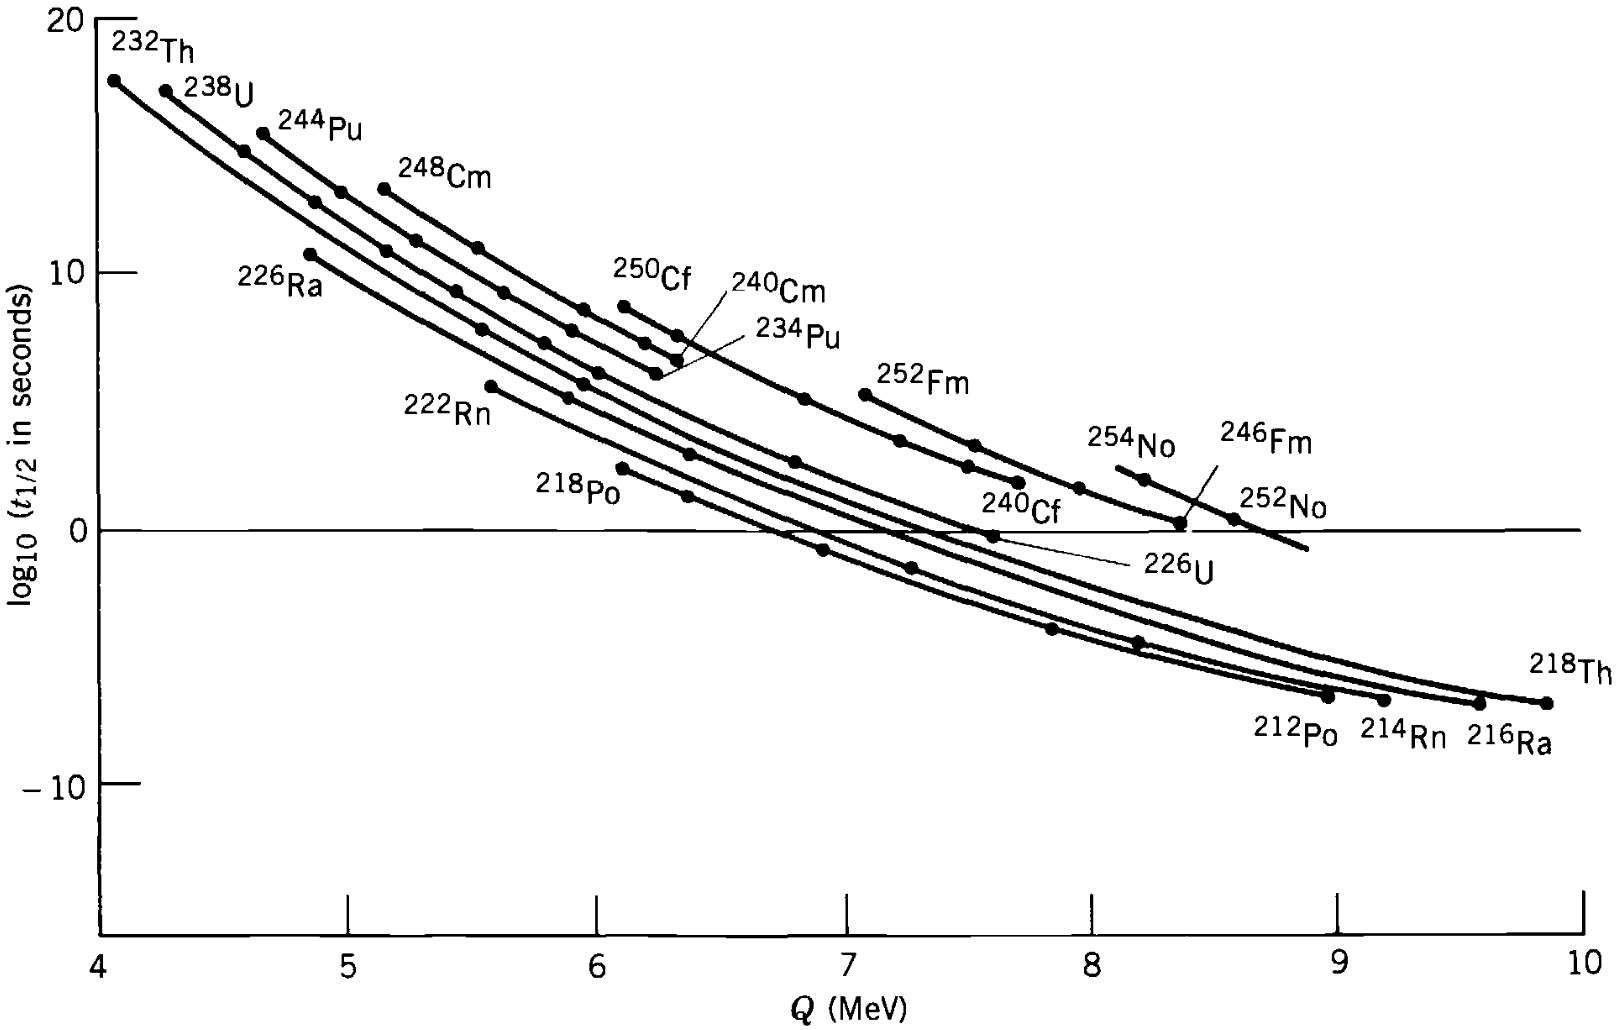
\includegraphics[width=0.75\textwidth]{geiger-nuttall.png}
	\caption{Legge di Geiger-Nuttal in famiglie isotopiche con nuclidi pari-pari.}
	\label{geiger-nuttall}
\end{figure}
\begin{figure}
	\centering
	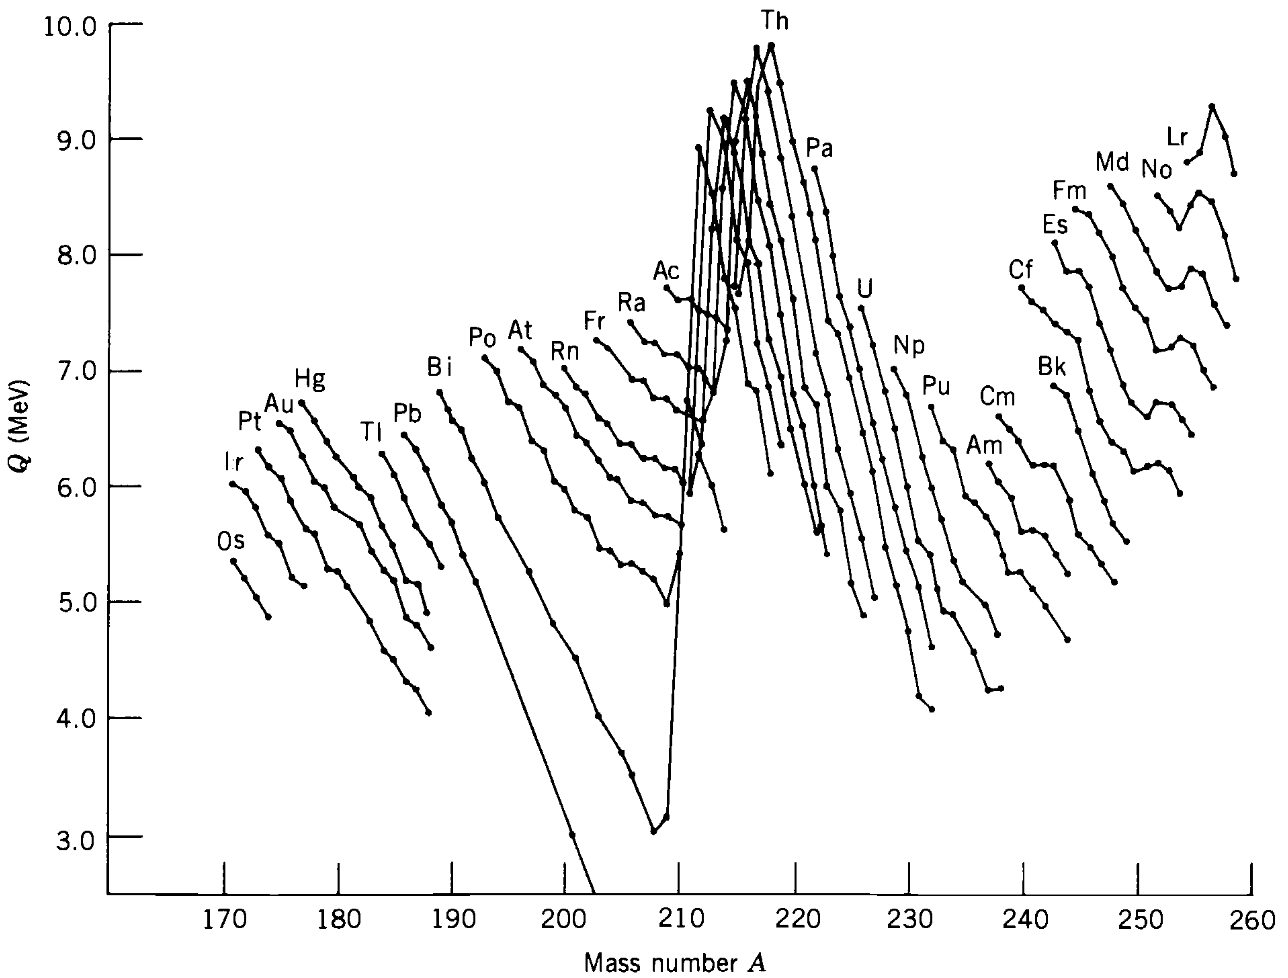
\includegraphics[width=0.75\textwidth]{gn-mass.png}
	\caption{Energia emessa per decadimento $ \alpha $ in famiglie isotopiche.}
	\label{gn-mass}
\end{figure}

\subsection{Teoria di Gamow}

La prima interpretazione teorica del decadimento $ \alpha $ fu data da Gamow nel 1929, qualche anno dopo le osservazioni di Geiger e Nuttall.\\
È possibile pensare alla particella $ \alpha $ come un corpo stabile preformato all'interno del nuclide $ \ch{^A X} $ che periodicamente di viene a trovare sulla superficie del nucleo, ad una distanza $ R \equiv R_{\ch{Y}} + R_{\alpha} $. Il moto della particella $ \alpha $ è determinato dal'energia potenziale d'interazione col nucleo, plottata in Fig. \ref{alpha-pot}, che fu proposta da Gamow essere:
\begin{equation}
	U(r) =
	\begin{cases}
		-V_0 & r < R \\
		\frac{2(Z-2)e^2}{4\pi \epsilon_0 r} & r > R
	\end{cases}
	\label{eq:2.12}
\end{equation}
Il senso fisico di tale espressione è che in prossimità del nucleo a prevalere è la forza nucleare, che ha natura attrattiva, mentre allontanandosi da esso prevale l'interazione coulombiana, che è repulsiva: si vede quindi la presenza di una barriera coulombiana in $ r = R $.\\
Con una trattazione classica la particella $ \alpha $ sarebbe emessa solo se $ E_{\alpha} > U(R) $ e ciò avverrebbe in un tempo comparabile al tempo di attraversamento del nucleo, ovvero $ t \sim R / v_{\alpha} = R \sqrt{2E_{\alpha} / m_{\alpha}} $: stimando $ R \approx 1.2\fm \left( (A - 4)^{1/3} + 4^{1/3} \right) $, per un nucleo con $ A \sim 230 $ e $ Q \sim 4\mev $ si trova $ R \sim 9\fm $ e $ t \sim 10^{-21}\,\text{s} $, ovvero un decadimento praticamente istantaneo. Ciò però non è quello che si osserva sperimentalmente.\\
Quantisticamente, invece, grazie all'effetto tunnel è possibile che anche le particelle $ \alpha $ con $ E_{\alpha} < U(R) $ (cosa che è praticamente sempre, dato che $ U(R) \sim 20\mev $) possono essere emesse con probabilità inderiori e dunque tempi di decadimento più lunghi.\\
È possibile svolgere il calcolo esplicitamente approssimando il potenziale coulombiano tra $ r = R $ ed $ r = R_{\alpha} $ (determinato da $ U(R_{\alpha}) = E_{\alpha} $) come una successione di barriere di potenziale di spessore $ dr $: dalla meccanica quantistica è noto che un'onda (particella) incidente su una barriera di potenziale di spessore $ L $ risulta in un'onda riflessa ed una trasmessa, le cui rispettive distribuzioni di probabilità (funzioni d'onda) sono determinate dai coefficienti di riflessione e trasmissione.

\begin{figure}[!hb]
	\centering
	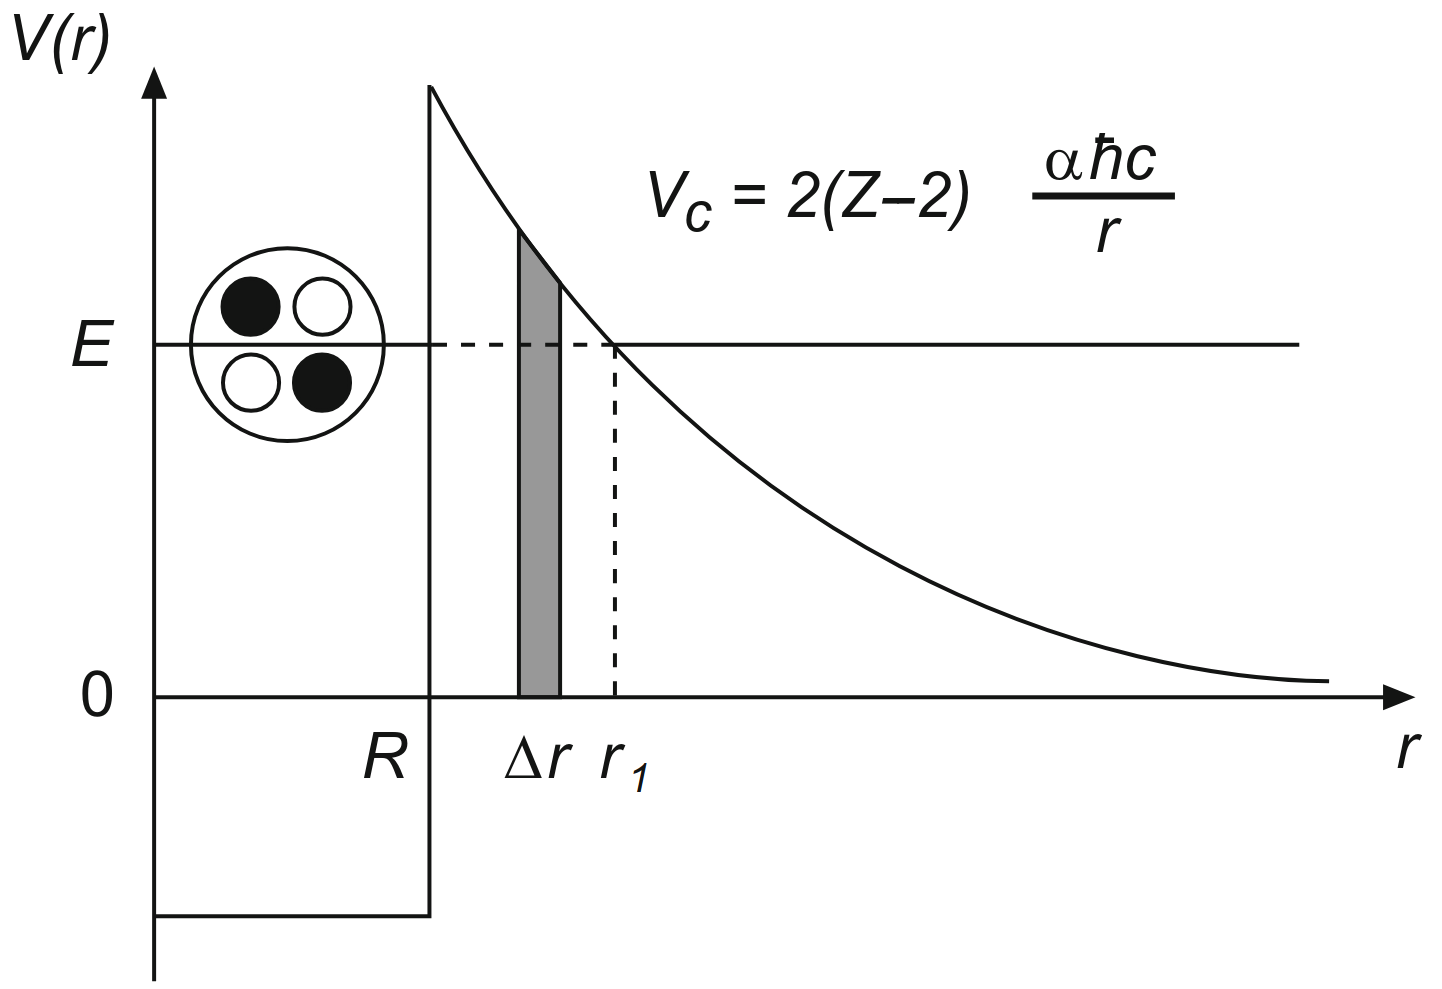
\includegraphics[width=0.60\textwidth]{alpha-pot.png}
	\caption{Potenziale d'interazione per il decadimento $ \alpha $.}
	\label{alpha-pot}
\end{figure}

Nel caso del decadimento $ \alpha $ è d'interesse solo il coefficiente di trasmissione nell'approssimazione $ E \ll V_0 $:
\begin{equation}
	T(E) = \left[ 1 + \frac{U_0^2}{4E (U_0 - E)} \sinh^2 \left( \frac{L}{\hbar} \sqrt { 2m (U_0 - E)} \right) \right]^{-1} \approx \frac{16 E (U_0 - E)}{U_0^2} e^{-2 \frac{L}{\hbar} \sqrt{2m (U_0 - E)}}
	\label{eq:2.13}
\end{equation}
Nel modello approssimato della successione di barriere di potenziale, quindi, si trova una probabilità di tunneling data da:
\begin{equation}
	P(E_{\alpha}) = \exp{\left[ -2 \int_{R}^{R_{\alpha}} dr \frac{1}{\hbar} \sqrt{2 m (U(r) - E_{\alpha}}) \right]} \eqdef e^{-2G}
	\label{eq:2.14}
\end{equation}
dove è stato definito il \textit{fattore di Gamow} $ G $. Svolgendo il calcolo col potenziale in Eq. \ref{eq:2.12} ed approssimando per una thick barrier $ R_{\alpha} \gg R $ (equivalente a $ E_{\alpha} \ll U(R) $, dato che dalla definizione $ R / R_{\alpha} = E_{\alpha} / U(R) $):
\begin{equation}
	\begin{split}
		G(E_{\alpha})
		&= \frac{2 (Z - 2) e^2}{\hbar} \sqrt{\frac{2m_{\alpha}}{E_\alpha}} \left[ \arccos \sqrt{\frac{R}{R_{\alpha}}} - \sqrt{\frac{R}{R_{\alpha}} - \frac{R^2}{R^2_{\alpha}}} \right]\\
		&\approx \frac{2 (Z - 2) e^2}{\hbar} \sqrt{\frac{2m_{\alpha}}{E_{\alpha}}} \left( \frac{\pi}{2} - \sqrt{\frac{R}{R_{\alpha}}} \right)
	\end{split}
	\label{eq:2.15}
\end{equation}
Questa espression mostra bene la fortissima dipendenza della probabilità di decadimento dall'energia della particella $ \alpha $: una piccola variazione di $ E_{\alpha} $ può portare $ P(E_{\alpha}) $ a variare di vari ordini di grandezza.\\
È anche possibile ricavare la legge di Geiger-Nuttall, dato che fenomenologicamente di può scrivere:
\begin{equation}
	\lambda = S \nu P(E_{\alpha})
	\label{eq:2.16}
\end{equation}
dove $ \lambda $ è la costante di decadimento, $ S $ è la probabilità che si formi una particella $ \alpha $ nel nucleo (può essere presa $ S \approx 1 $) e $ \nu $ è la knocking frequency, ovvero la frequenza con cui la particella $ \alpha $ urta con la barriera coulombiana. Si può stimare $ \nu $ a partire dal tempo che impiega la particella $ \alpha $ ad attraversare il nucleo (già trovato in precedenza): $ \nu \sim t^{-1} \sim 10^{21} \,\text{Hz} $. Dall'Eq. \ref{eq:2.16} si ha:
\begin{equation}
	\ln \lambda = \ln S + \ln \nu - 2 G(E_{\alpha}) \sim a(Z) - b \frac{Z}{\sqrt{E_{\alpha}}}
	\label{eq:2.17}
\end{equation}
che, ricordando che $ t_{1/2} = \frac{\ln 2}{\lambda} $, è proprio la legge di Geiger-Nuttall.\\
Ovviamente tutte queste relazioni sono qualitative e non quantitative, dato che sono state fatte alcune approssimazioni dalle quali la realtà si discosta notevolmente, prima su tutti la simmetria sferica: i nuclidi pesanti hanno forme notevolmente deformate (tendenti ad ellissoidi di rotazione), dunque le loro emissioni presentano notevoli anisotropie nella distribuzione angolare di particelle $ \alpha $.

\subsection{Spettri}

Per molti nuclidi che decadono tramite decadimento $ \alpha $ è possibile la presenza di più branch di decadimento, con percentuali di decadimento basse rispetto a quella dominante, che non portano direttamente allo stato fondamentale del nucleo figlio, ma a qualche suo stato eccitato: ciascuna di queste branch ha una propria energia di decadimento (deve essere sempre mono-energetico), e solitamente la branch con l'energia più alta è quella che va a popolare lo stato fondamentale del nucleo figlio.\\
Lo studio degli spettri di decadimento così prodotti (ad esempio immettendo le particelle $ \alpha $ in uno spettrometro magnetico) è importante per studiare i vari livelli energetici del nucleo figlio, specialmente nel caso in cui esso appartenga ad una specie nucleare di difficile sintesi.

\subsection{Cluster decay}

Spesso, quando un nuclide risulta instabile rispetto al decadimento per $ \ch{^4 He} $, esso lo è anche rispetto a quello per $ \ch{^8_4 Be} $, $ \ch{^{12}_6 C} $ ed altri nuclei, tendenzialmente formati da più particelle $ \alpha $, i cosiddetti \textit{nuclear clusters}. Anche questi sono sistemi particolarmente stabili preformati nel nucleo e, per un nuclear cluster di $ n $ particelle $ \alpha $, si può approssimare $ Q_n \sim Q_{\alpha}^n $: di conseguenza, per la legge di Geiger-Nuttall, i tempi di decadimento sono enormemente più lungi rispetto a quelli del decadimento $ \alpha $, con conseguenza che i branching ratios sono praticamente trascurabili, sebbene occasionalmente questi cluster decays vengano osservati e siano stati ampiamente studiati.

\section{Fissione}

Dopo la scoperta del neutrone da parte di Chadwick nel 1932, furono condotti numerosi esperimenti nei quali vari nuclidi venivano irraggiati con neutroni: in particolare, Fermi et al. studiarono la radioattività a seguito della neutron capture, ottenendo il Nobel nel 1938 per gli studi sul decadimento $ \beta^- $, mentre Meitner e Hahn osservarono la fissione negli elementi transuranici.

\paragraph{Neutroni}

Si utilizza una specifica terminologia per classificare i neutroni in base alla loro energia $ E_n $:
\begin{enumerate}
	\item high energy neutrons: $ E_n > 100\mev $;
	\item fast neutrons: $ 100\kev < E_n < 100\mev $;
	\item epithermal neutrons: $ 0.1\ev < E_n < 100\kev $;
	\item thermal/slow neutrons: $ 1\,\text{meV} < E_n < 0.1\ev $,
	\item cold/ultracold neutrons: $ E_n < 1\,\text{meV} $.
\end{enumerate}
Come si può vedere in Fig. \ref{fission-cs}, sperimentalmente si trova che i neutroni a basse energie, specialmente i thermal neutrons, sono quelli più efficaci per indurre reazioni di fissione nucleare.

\begin{figure}
	\centering
	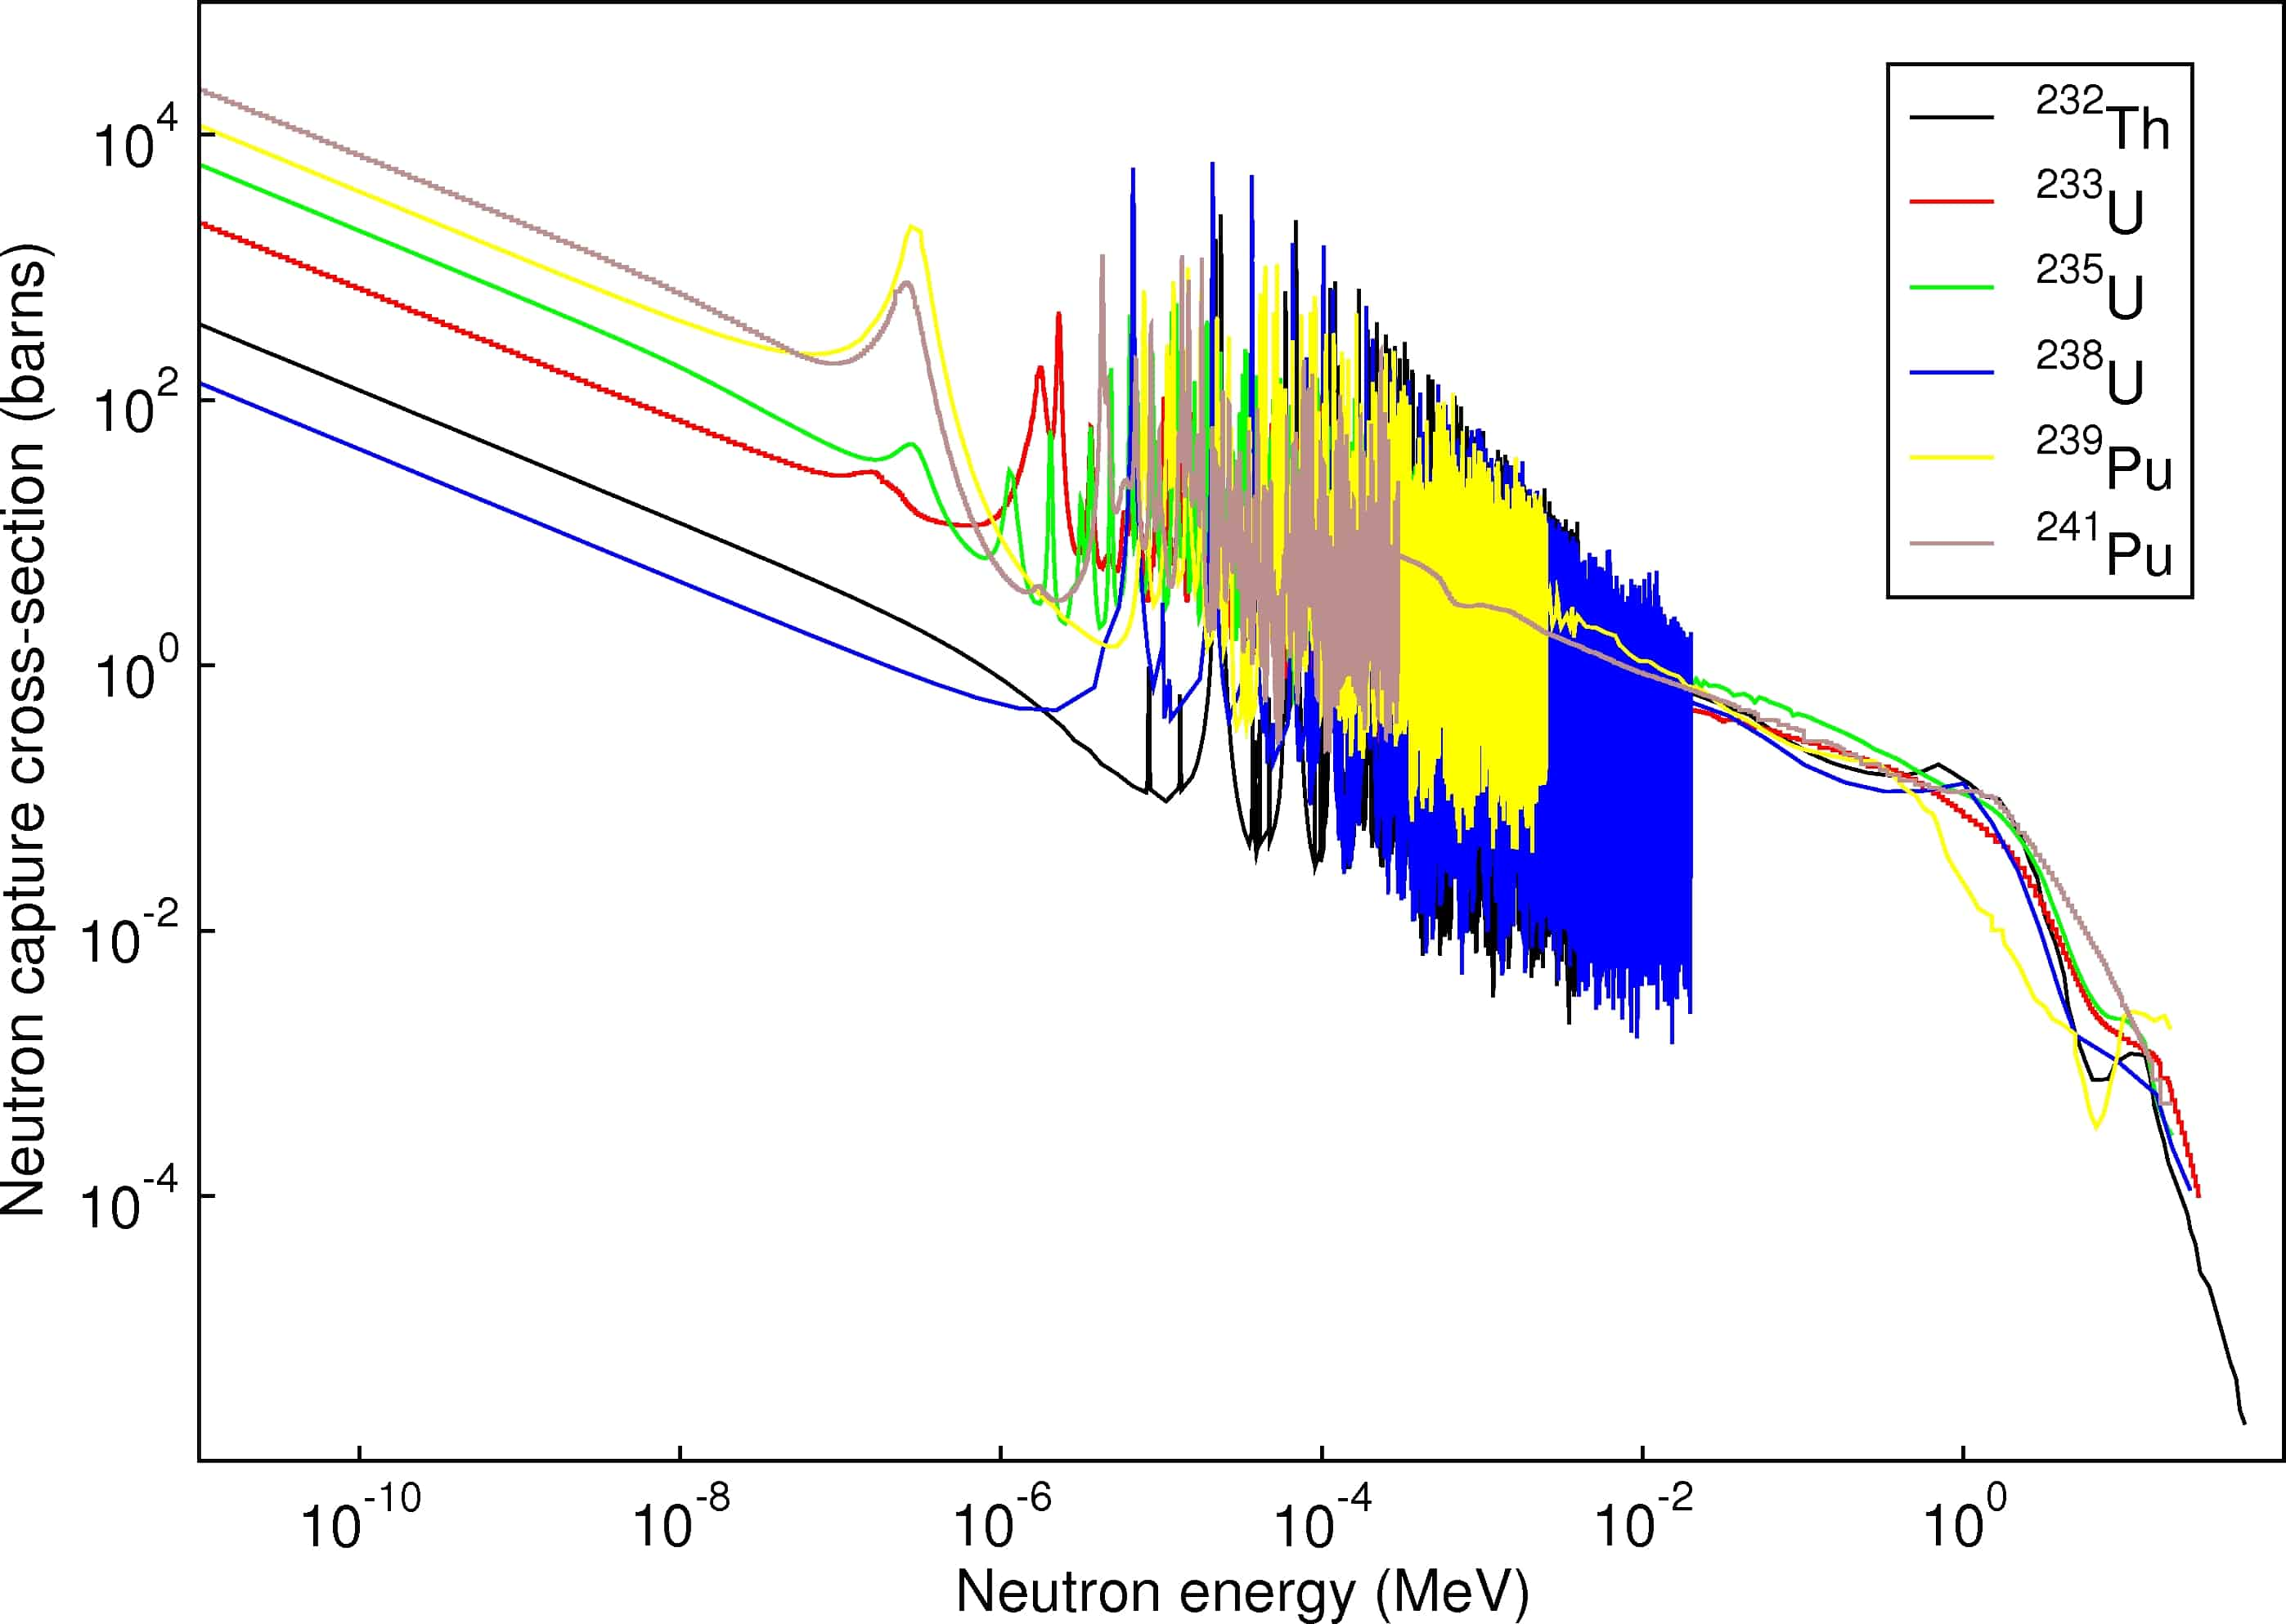
\includegraphics[width=0.75\textwidth]{fission-cs.jpg}
	\caption{Neutron-induced fission cross-section.}
	\label{fission-cs}
\end{figure}
\begin{figure}
	\centering
	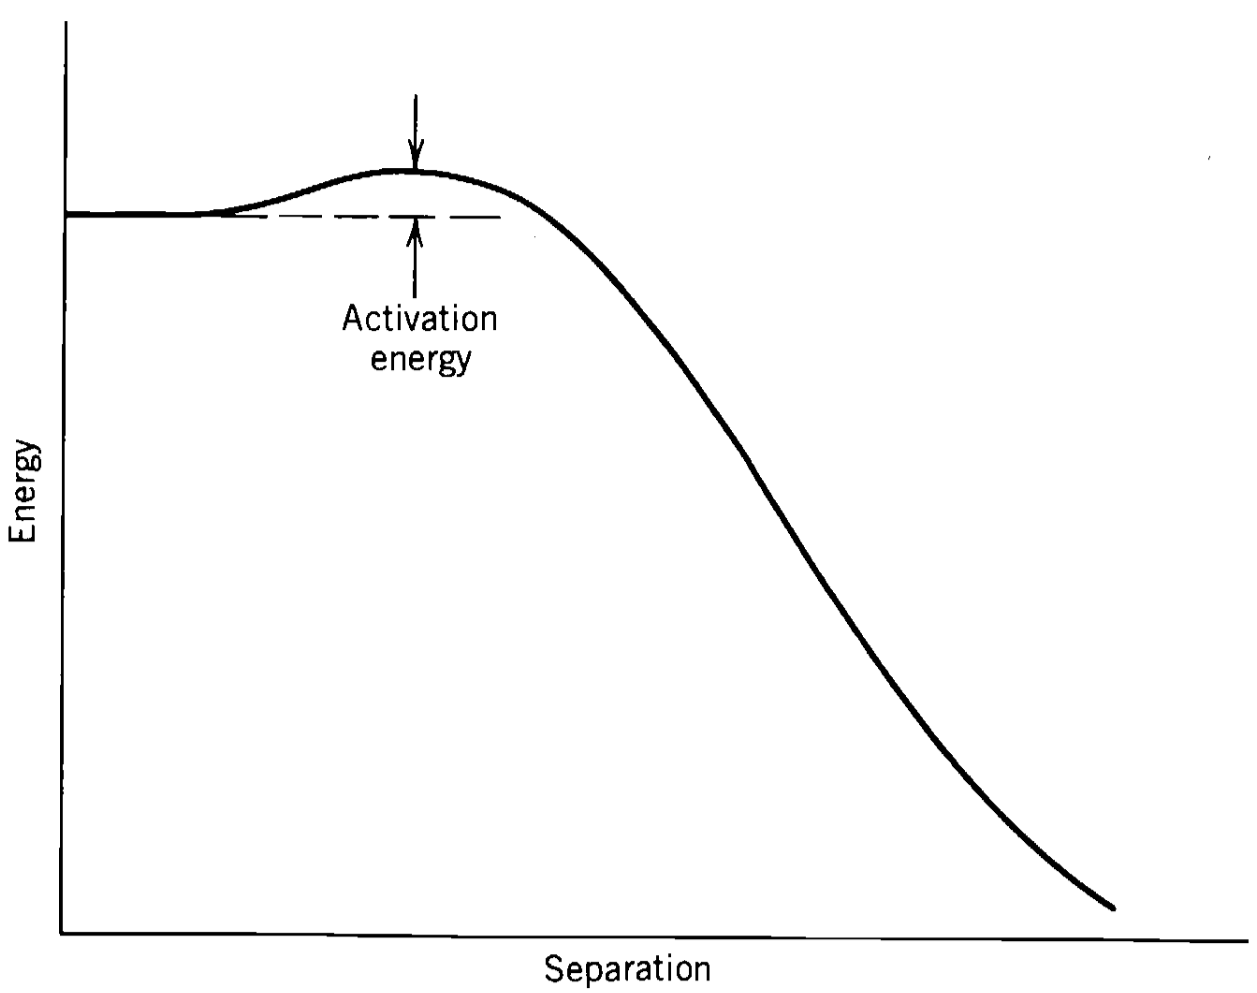
\includegraphics[width=0.75\textwidth]{fission-pot.png}
	\caption{Coulomb potential in a fissioning nucleus.}
	\label{fission-pot}
\end{figure}

\subsection{Fissione spontanea}

La tendenza dei nuclei pesanti a fissionare è evidente dall'andamento della binding energy rispetto ad $ A $ (Fig. \ref{bind-en}): ad esempio, se si considera la fissione dell'uranio $ \ch{^{235}_{92} U} \rightarrow \ch{^{90}_{36} Kr} + \ch{^{142}_{56} Ba} + 3 n $, il $ Q $-value della reazione è $ 166.73\mev $, dunque è una reazione energeticamente fortemente favorita. Va però notato che il decay branch per decadimento $ \alpha $ è fortemente dominante in natura, basta confrontare, ad esempio, i seguenti decadimenti:
\begin{equation*}
	\begin{split}
		\ch{^{238}_{92} U} \xrightarrow{4\,\text{Gy}} \ch{^{234}_{90} Th} + \alpha &\qquad \ch{^{238}_{92} U} \xrightarrow{\sim 10^7\,\text{Gy}} \ch{^{140}_{54} Xe} + \ch{^{96}_{38} Sr} + 2n\\
		\ch{^{235}_{92} U} \xrightarrow{0.7\,\text{Gy}} \ch{^{231}_{90} Th} + \alpha &\qquad \ch{^{235}_{92} U} \xrightarrow{\sim 10^8\,\text{Gy}} \ch{^{142}_{56} Ba} + \ch{^{90}_{36} Kr} + 3n
	\end{split}
\end{equation*}
La fissione è osservata solo in nuclei pesanti (il nuclide fissile più leggero è $ \ch{^{226}_{88} Ra} $), e la fissione spontanea diventa il decay mode dominante solo in nuclidi con $ A \ge 250 $.\\
Ciò che inibisce la fissione è una barriera coulombiana analoga a quella del decadimento $ \alpha $: in questo caso, però, essa ha un andamento liscio (in senso analitico), com'è possibile vedere in Fig. \ref{fission-pot}. L'energia necessaria affinché i due prodotti della fissione (supposti preformati) oltrepassino la barriera coulombiana è, nella maggior parte dei casi, troppo alta per rendere la fissione un decay mode significativo; a livello teorico, dovrebbero esistere anche dei nuclidi in cui la barriera si annulla, ovvero in cui i due prodotti hanno sempre l'energia necessaria per superarla, e tali nuclidi dovrebbero fissionare istantaneamente: naturalmente essi non esistono in natura, e si dovrebbero trovare attorno ad $ A = 300 $.\\
L'altezza della barriera coulombiana rispetto all'energia del ground state è detta activation energy ed è possibile calcolarla sia assumendo il modello semplificato a goccia sia tenendo conto degli effetti delle shell nucleari: entrambi i casi sono pllottati in Fig. \ref{act-en}.

\begin{figure}
	\centering
	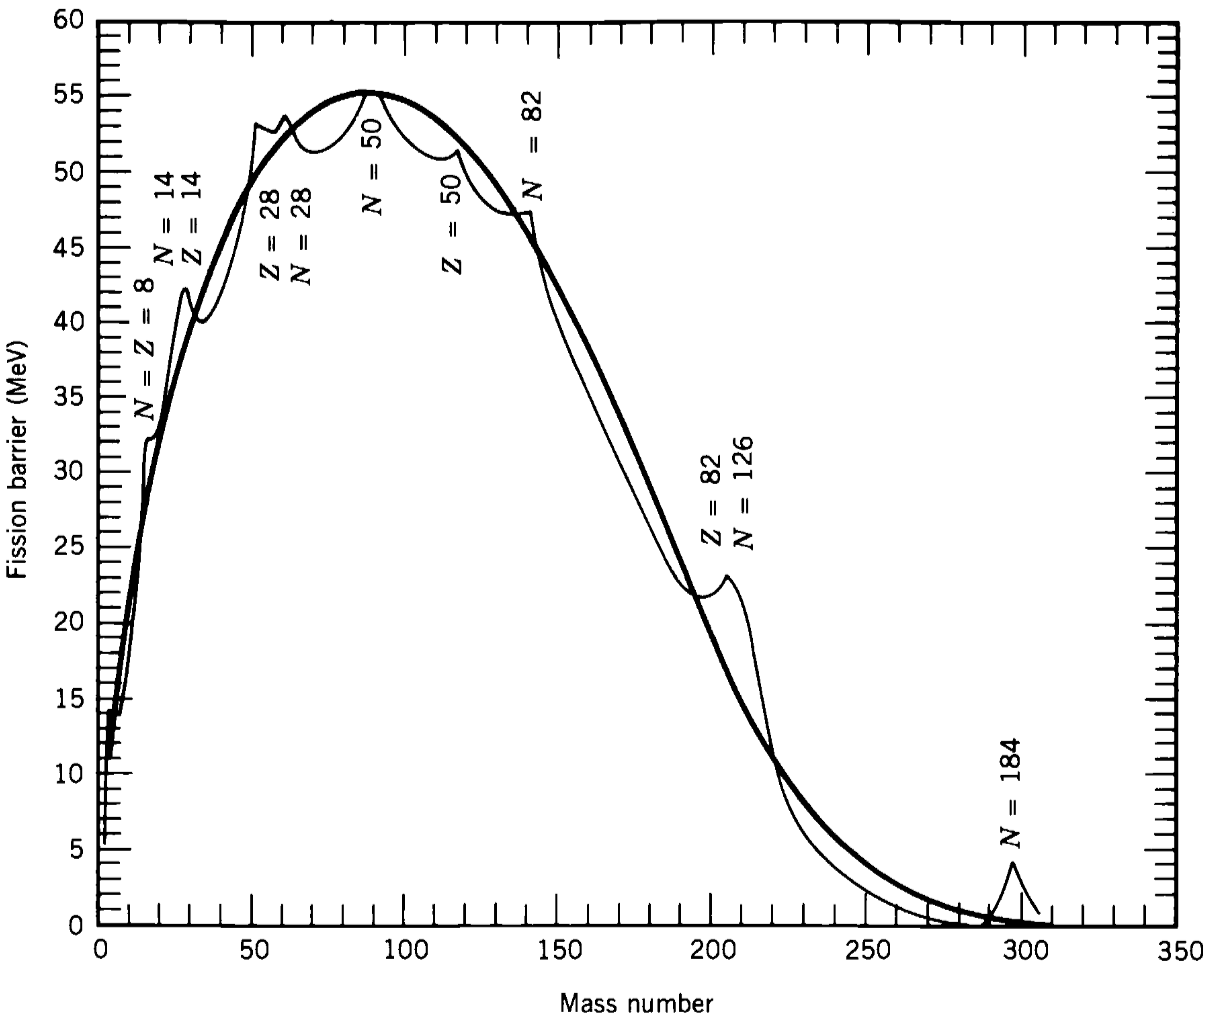
\includegraphics[width=0.65\textwidth]{act-en.png}
	\caption{Activation energy of nuclear fission.}
	\label{act-en}
\end{figure}
\begin{figure}
	\centering
	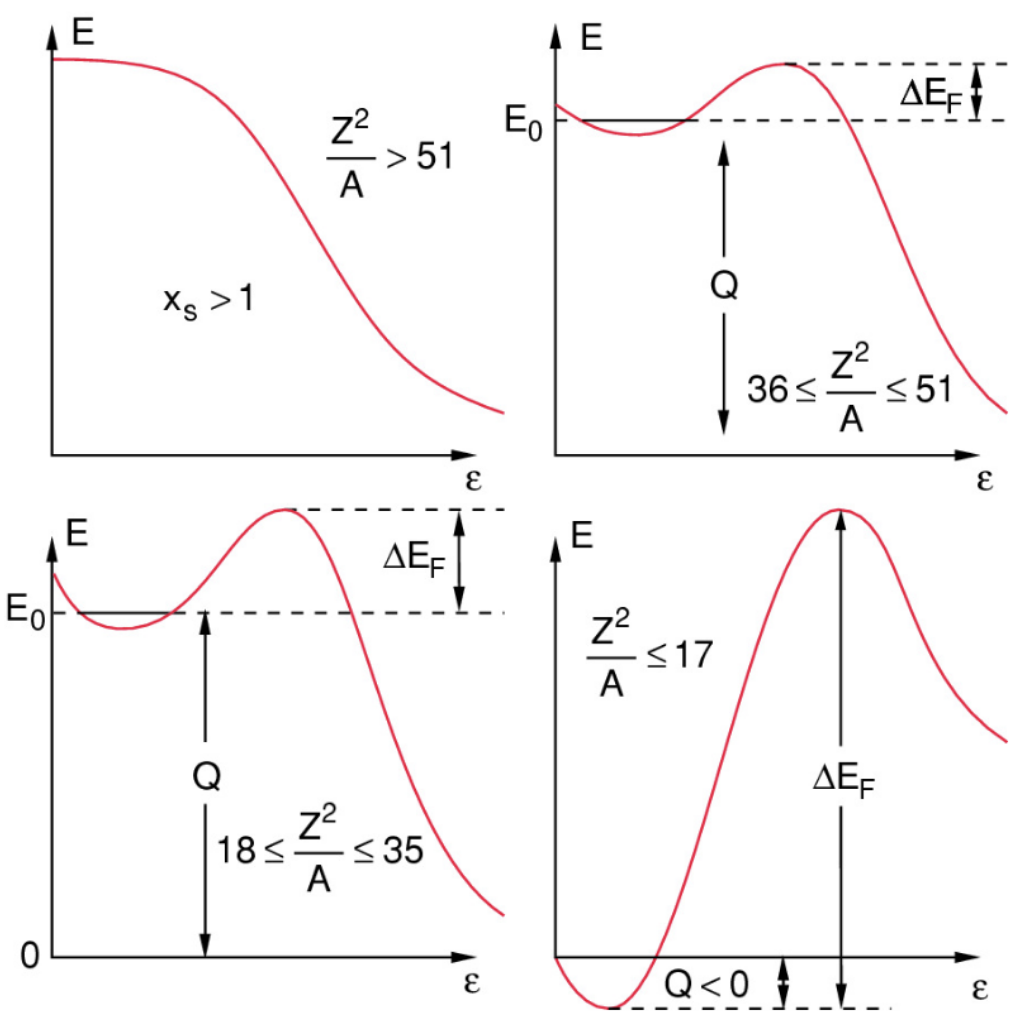
\includegraphics[width=0.60\textwidth]{act-en-z.png}
	\caption{Potential barrier as a funzion of the deformation parameter for various fissility values.}
	\label{act-en-z}
\end{figure}

\paragraph{Liquid drop model}

Semplificando, questo modello considera solo le proprietà nucleari medie, assumendo un nuclide sferico nel suo ground state. Nel caso di un nucleo fissile, l'instabilità porta ad una deformazione del nuclide in un ellissoide: assumendo il raggio iniziale $ R $ e l'eccentricità dell'ellissoide $ \varepsilon $, si possono calcolare i semiassi come:
\begin{equation}
	a = R \left( 1 + \varepsilon \right) \qquad b = R \left( 1 + \varepsilon \right)^{-1/2}
	\label{eq:2.18}
\end{equation}
Si vede dunque che il volume $ V = \frac{4}{3}\pi R^3 = \frac{4}{3} \pi ab^2 $ rimane inalterato, mentre la superficie varia di un fattore approssimabile ad $ \varepsilon $: $ S = 4\pi R^2 \left( 1 + \frac{2}{5} \varepsilon^2 + \dots \right) $; analogamente, si mostra che l'energia d'interazione coulombiana varia di un fattore $ \left( 1 - \frac{1}{5} \varepsilon^2 + \dots \right) $.\\
Dalla formula semi-empirica di Weizsäcker (Eq. \ref{eq:1.30}) deriva che, a seguito della deformazione, la binding energy varia di:
\begin{equation}
	\Delta B = - a_S A^{2/3} \left( 1 + \frac{2}{5} \varepsilon^2 + \dots \right) - a_C \frac{Z^2}{A^{1/3}} \left( 1 - \frac{1}{5} \varepsilon^2 + \dots \right) \approx \left( -\frac{2}{5} a_S A^{2/3} + \frac{1}{5} a_C \frac{Z^2}{A^{1/3}} \right) \varepsilon^2
	\label{eq:2.19}
\end{equation}
Se $ \Delta B > 0 $, il nucleo risulta instabile rispetto alla deformazione e fissiona, dunque si trova una condizione per la fissione spontanea:
\begin{equation}
	\Chi \defeq \frac{a_C}{2a_S} \frac{Z^2}{A} > 1
	\label{eq:2.20}
\end{equation}
dove è stata definita la fissility $ \Chi $. Utilizzando i valori di $ a_S $ ed $ a_C $ interpolati si trova la condizione $ Z^2 / A > 51 $, ovvero $ Z > 114 $ e $ A > 270 $; al di sotto di questi valori la fissione è possibile solo fornendo la necessaria energia di attivazione (vedere Fig. \ref{act-en-z}).\\
Bisogna specificare che per $ Z^2 / A > 51 $ la fissione spontanea è istantanea, mentre per nuclidi con $ Z^2 / A \lesssim 51 $ è possibile anche una delayed fission per effetto tunnel (a causa della repulsione tra protoni), analogamente al decadimento $ \alpha $, ma nella maggior parte dei casi quest'ultimo è dominante.
Infine, si può notare in Fig. \ref{fission-lt} come i tempi di decadimento aumentino al diminuire di $ Z^2 / A $.

\begin{figure}[!hb]
	\centering
	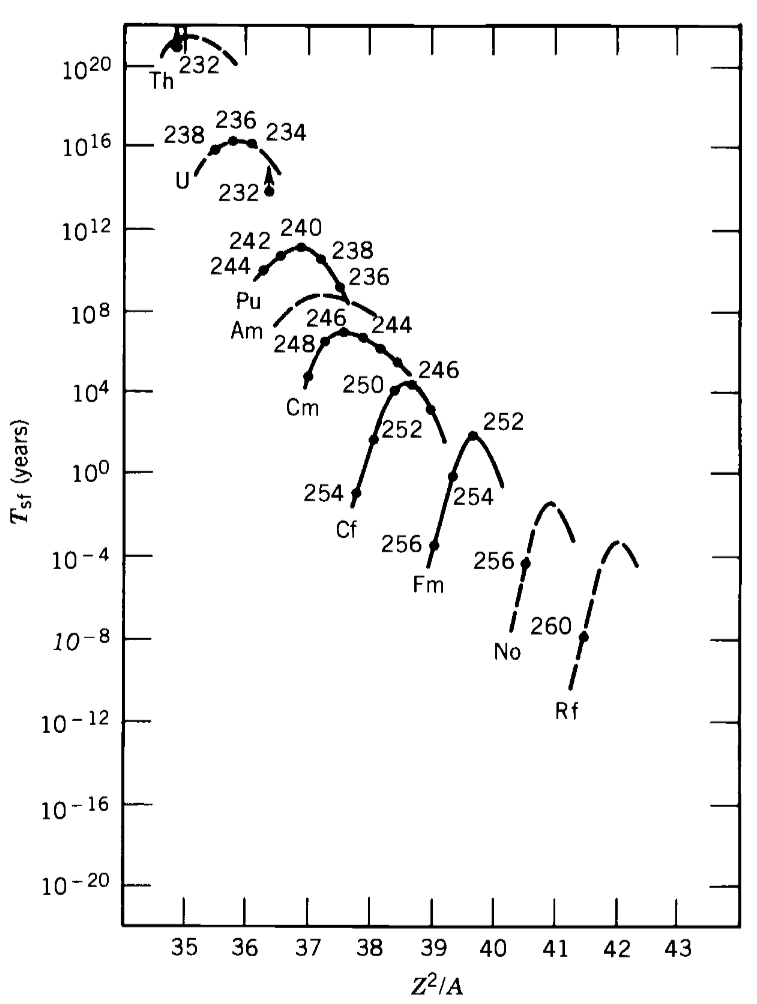
\includegraphics[width=0.80\textwidth]{fission-lt.png}
	\caption{Lifetimes for spontaneous fission.}
	\label{fission-lt}
\end{figure}

\subsection{Fissione indotta}

Dato che i neutroni non sono affetti dal potenziale coulombiano, è possibile indurre la fissione di un nuclide facendolo scatterare con un neutrone termico. Bisogna però notare una differenza tra la fissione di nuclidi pari-pari e nuclidi pari-dispari, dovuta al termine di pairing nella formula di Weizsäcker (Eq. \ref{eq:1.30}).\\
Si considerino ad esempio due campioni di $ \ch{^{235}_{92} U} $ e $ \ch{^{235}_{92} U} $ e li si irraggi con neutroni termici:
\begin{enumerate}
	\item $ \ch{^{235}_{92} U} + n \rightarrow \ch{^{236}_{92} U}^* $: $ Q = 6.5\mev > \Delta E_F = 6.1\mev $;
	\item $ \ch{^{238}_{92} U} + n \rightarrow \ch{^{239}_{92} U}^* $: $ Q = 4.8\mev < \Delta E_F = 6.4\mev $;
\end{enumerate}
Si vede dunque che la fissione di $ \ch{^{235}_{92} U} $ può avvenire con neutroni termici, mentre per quella di $ \ch{^{238}_{92} U} $ sono necessari neutroni veloci. Ciò è dovuto al fatto che i nuclidi pari-pari sono energeticamente favoriti, dunque il termine di pairing favorisce processi da pari-dispari a pari-pari, mentre ostacola quelli da pari-pari a pari-dispari: nel caso considerato, infatti, la differenza di energia ammonta a $ \Delta E = \delta (236^{-1/2} + 238^{-1/2}) = 1.5\mev $.\\
È interessante notare che $ \ch{^{235}_{92} U} $ e $ \ch{^{238}_{92} U} $ sono gli unici isotopi dell'uranio rimasti in natura, con abbondanze isotopiche rispettivamente del $ 0.72\% $ e $ 99.28\% $.

\subsection{Caratteristiche}

Il processo di fissione del nuclide non presenza grosse differenze tra il caso spontaneo e quello indotto: in maniera quasi istantanea ($ \sim 10^{-17}\,\text{s} $) il nucleo si deforma radicalmente andando a formare i due frammenti di fissione (sono possibili fissioni ternarie ma sono estremamente rare), i quali si separano in tempi brevissimi ($ \sim 10^{-14}\,\text{s} $): questi sono nuclidi molto neutron-rich, dunque espellono i neutroni con energie di legame superiori all'energia di legame media, andando così a formare i prodotti di fissione; quest'ultimi possono decadere tramite decadimenti $ \beta $ e $ \gamma $, con tempi su una scala dai secondi ai milioni di anni, muovendosi verso la valle di stabilità.

\subsubsection{Asimmetria di fissione}

I due frammenti altamente eccitati in cui si separa il nucleo a seguito della fissione non sono uguali, ma presentano una notevole asimmetria; per di più, variando il nuclide fissile si osserva che la distribuzione dei frammenti pesanti rimane praticamente inalterata, mentre la massa in eccesso viene inglobata dai frammenti leggeri (vedere Fig. \ref{fission-md}).\\
Ciò può essere spiegato dal fatto che la fissione, sebbene trattata in maniera elementare utilizzando il liquid drop model, risente in realtà degli effetti delle shell nucleari: come si può notare in Fig. \ref{fission-asimm}, la distribuzione dei frammenti pesanti si sovrappone ad una regione di completamento di shell nucleari, con la presenza anche del nuclide doubly-magic $ \ch{^{132}_{50} Sn_{82}} $, che ha una configurazione estremamente stabile; tutto ciò non accade, invece, per la distribuzione dei frammenti leggeri, i quali non si sovrappongono a nessun magic nucleus.\\
Circa metà dei prodotti di fissione decadono in meno di un anno, mentre i restanti possono avere tempi di decadimento anche di milioni di anni: questi formano le scorie radioattive.\\
I prodotti di fissione sono molto neutron-rich, dunque per la maggior parte sono instabili per decadimento $ \beta^- $: la fissione nucleare è un importante strumento di ricerca per la regione $ \beta^- $-instabile, difficilmente raggiungibile con altri metodi: i prodotti di fissione possono dar luogo ad intere catene di decadimenti $ \beta^- $.

\begin{figure}
	\centering
	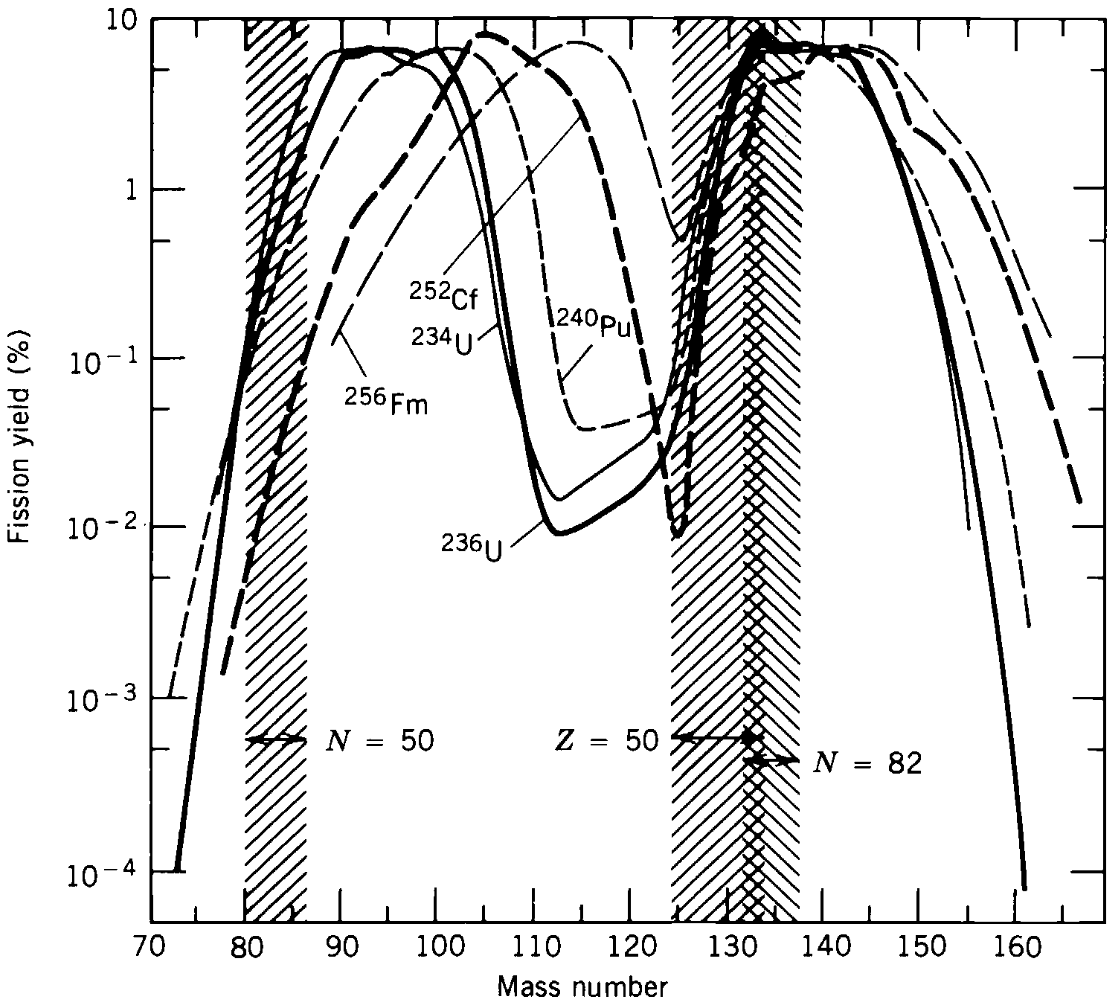
\includegraphics[width=0.60\textwidth]{fission-asimm.png}
	\caption{Asimmetry in fission products.}
	\label{fission-asimm}
\end{figure}
\begin{figure}
	\centering
	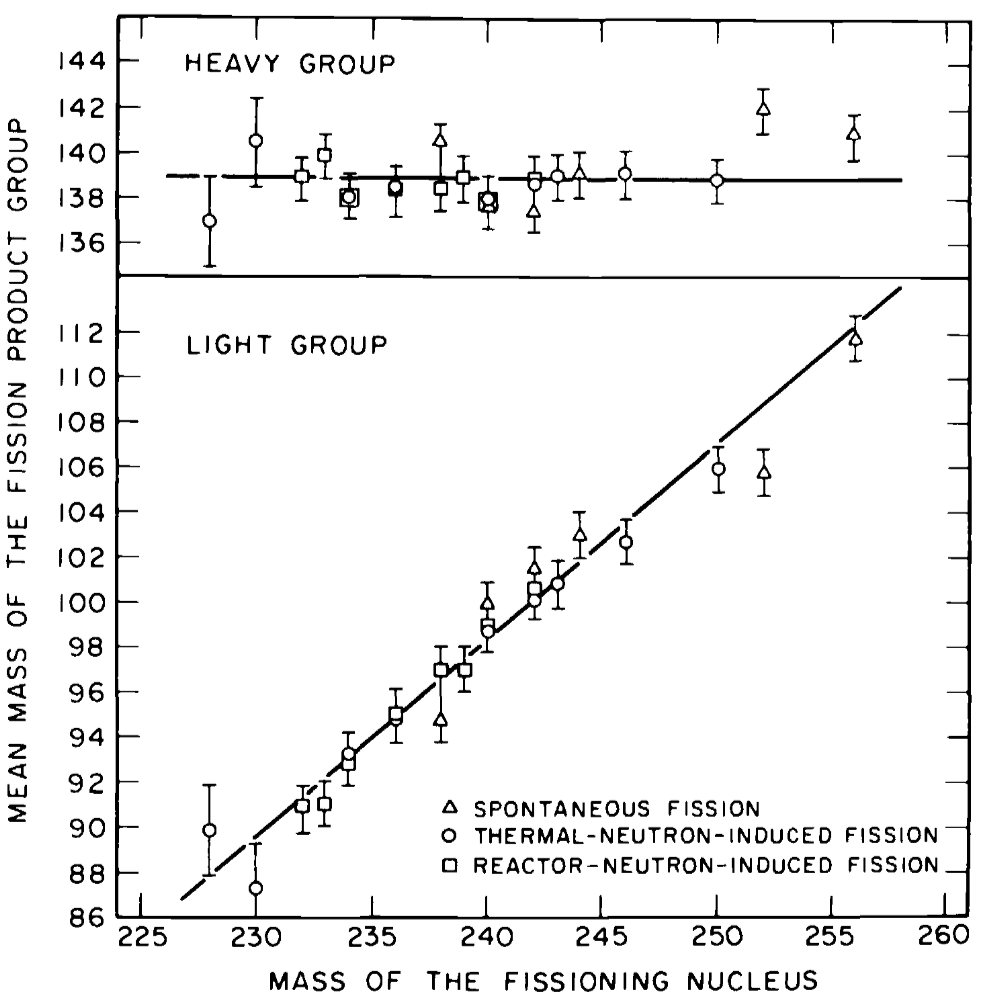
\includegraphics[width=0.60\textwidth]{fission-md.png}
	\caption{Distributions of light and heavy fission products.}
	\label{fission-md}
\end{figure}

\subsubsection{Emissione di neutroni}

I neutroni prodotti dalla fissione di un nuclide si possono distinguere in due categorie: prompt neutrons and delayed neutrons.\\
I prompt neutrons vengono emessi praticamente in contemporanea al processo di fissione, venendo emessi dal nuclide fissile e dai frammenti di fissione: il numero di prompt neutrons viene indicato come $ \nu_n $ e generalmente si ha $ \langle \nu_n \rangle \approx 2.4 $.\\
La distribuzione di prompt neutrons in base alla loro energia cinetica è una distribuzione di Maxwell, mentre $ \nu_n $ si distribuisce secondo una gaussiana indipendentemente dalla fissione considerata, come visibile in Fig. \ref{n-neut-dist}: i prompt neutrons vengono prodotti con energia di circa $ 2\mev $, in media.\\
I delayed neutrons, d'altro canto, sono quelli prodotti nelle decay chains iniziate dai prodotti di fissione, solitamente tra $ 0.2\,\text{s} $ e $ 60\,\text{s} $ dopo la fissione, e costituiscono appena l'$ 1\% $ dei neutroni totali prodotti dalla fissione.

\begin{figure}[!b]
	\centering
	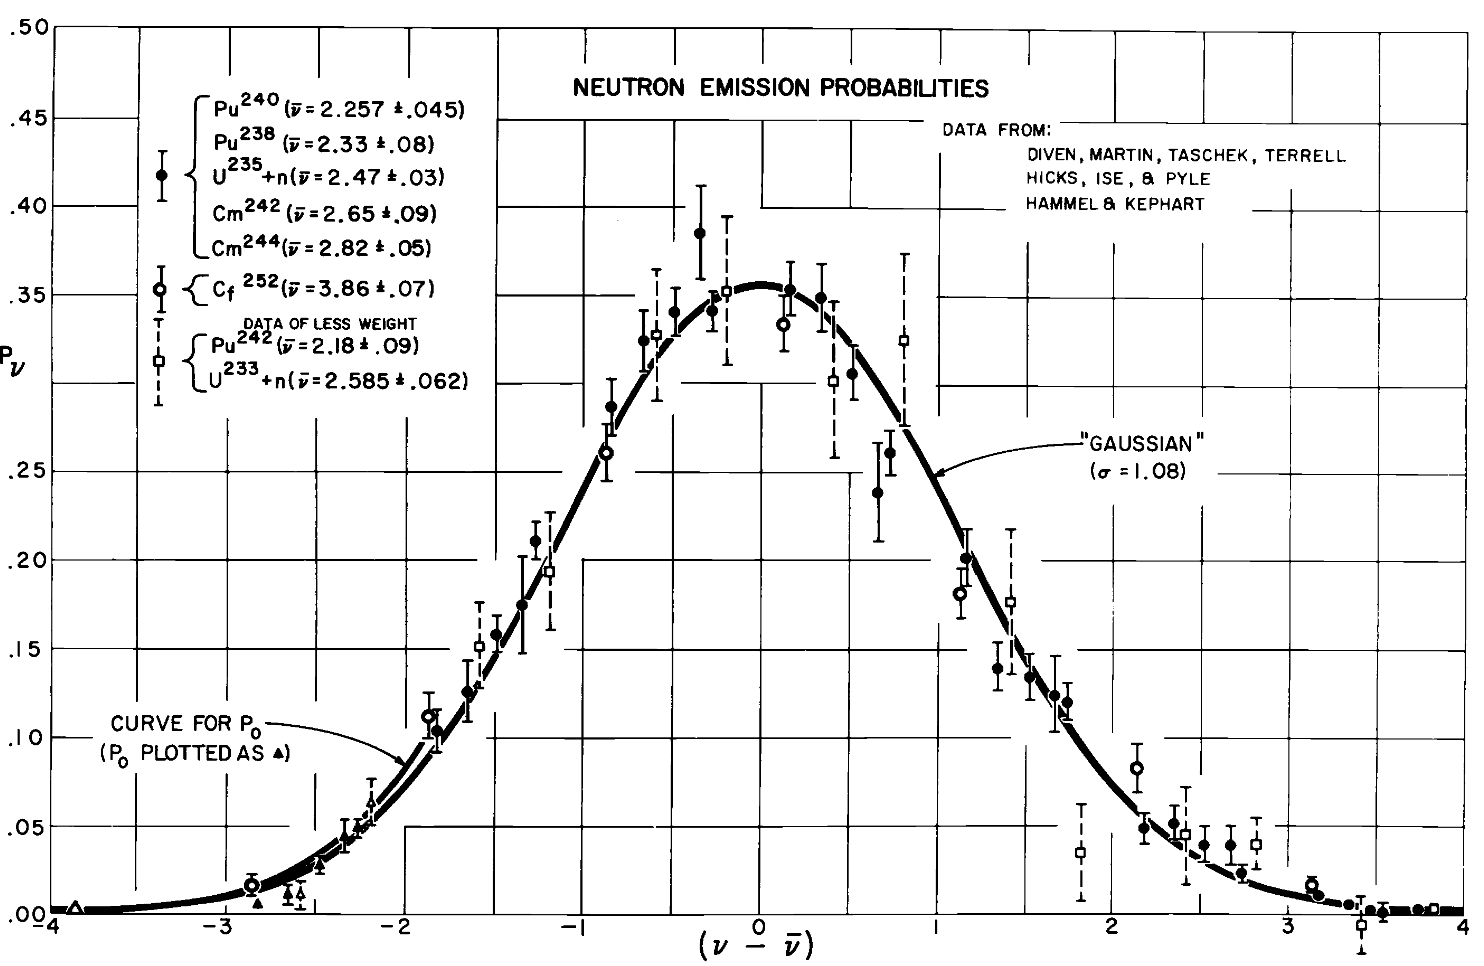
\includegraphics[width=0.75\textwidth]{n-neut-d.png}
	\caption{Prompt neutrons' number distribution.}
	\label{n-neut-dist}
\end{figure}

\subsubsection{Bilancio energetico}

Considerando, ad esempio, la fissione del $ \ch{^{235}_{92} U} $, i $ 210\mev $ di energia rilasciata vengono ripartiti nel seguente modo:
\begin{enumerate}
	\item frammenti di reazione: $ \ch{Y}_{\text{small}} \approx 100\mev $ e $ \ch{Y}_{\text{large}} \approx 70\mev $;
	\item prompt emissions: neutrons $ \approx 5\mev $ e fotoni $ \approx 7\mev $;
	\item decadimenti: $ \beta^- \approx 20\mev $ (di cui $ \approx 12\mev $ persi in neutrini) e $ \gamma \approx 8\mev $.
\end{enumerate}
La differenza tra i due frammenti è dovuta alla conservazione del momento lineare: trascurando i neutroni si ha $ m_1 \ve{v}_1 = m_2 \ve{v}_2 $, dunque $ K_1 / K_2 = m_2 / m_1 $, ovvero il frammento leggero acquista la maggior parte del'energia cinetica disponibile.

\subsection{Applicazioni}

\subsubsection{Studio della stuttura nucleare}

Dato che la fissione produce nuclidi neutron-rich eccitati molto esotici, essa può essere usata per studiare una zona difficilmente popolabile della nuclear chart, quella $ \beta^- $-instabile.\\
Inoltre, a partire dalla fissione è possibile ottenere la cosiddetta spallazione del nuclide fissile: quando il l'energia della particella proiettile è molto elevata la fissione produce frammenti multipli. Essendo il processo non più binario, la distribuzione dei frammenti non è più a doppia campana (come in Fig. \ref{fission-asimm}), ma si va a popolare anche la conca centrale: più è alta l'energia del proiettile, più saranno i frammenti di masse intermedie prodotti.\\
Questo, ad esempio, è ciò che avviene nell'esperimento ISOLDE al CERN: nuclei esotivi vengono prodotti con irraggiamento di protoni, i quali, provenendo da LHC, hanno energie dell'ordine di $ 1.5\gev $.

\subsubsection{Reattori a fissione}

Il funzionamento dei reattori a fissione nucleare si basa sulle reazioni a catena dell'uranio: queste avvengono poiché la fissione di $ \ch{^{235}_{92} U} $ produce in media 3 neutroni, i quali potenzialmente possono dar luogo ad ulteriori fissioni.\\
Il problema principale è che $ \ch{^{235}_{92} U} $ richiede un neutrone termico per fissionare, mentre i neutroni prodotti dalla fissione sono neutroni veloci: per rallentare questi neutroni, è necessario alternare nel reattore strati di materiale fissile a strati di materiale moderatore. Quest'ultimo solitamente è costituito da acqua o da grafite, materiali leggeri con una cross-section elevata per scattering neutronico (elastico) ai quali viene ceduta una grande frazione dell'energia cinetica.\\
È inoltre necessaria, come materiale fissile, una miscela di uranio con almeno il $ 3\% $ di $ \ch{^{235}_{92} U} $: per fare ciò, è necessario arricchire l'uranio estratto in natura. Il $ \ch{^{238}_{92} U} $ non è inerte, ma può fissionare quando dei neutroni veloci sfuggono alle barre di moderazione.\\
Per mantenere la reazione sotto controllo bisogna avere il giusto numero di neutroni: se non vengono prodotti abbastanza neutroni dalle fissioni la catena non riesce ad autosostenersi, mentre se ne vengono prodotti troppi c'è il rischio che essa non sia più controllabile ed esploda esponenzialmente. In particolare, data una certa massa di materiale fissile, si definisce il neutron reproduction factor $ k $ come il rapporto tra i numeri di neutroni fissili (quelli che effettivamente danno luogo a fissioni) di due generazioni successive di nuclidi fissili a catena avviata: la massa si dice critica se $ k = 1 $, supercritica se $ k > 1 $ e subcritica se $ k < 1 $.\\
L'obbiettivo, in un reattore a fissione, è mantenere il materiale fissile in stato critico, dunque controllabile: per mantenere la catena sotto controllo si utilizzano delle barre fatte di materiale ad alto potere d'assorbimento di neutroni (ad esempio bario, boro, cadmio, indio etc.), le quali possono essere inserite all'interno del materiale fissile per bloccare totalmente o in parte la reazione.\\
Un altro parametro importante nella caratterizzazione di un reattore a fissione è il numero medio di neutroni termici fissili: infatti, non tutti i neutroni termici prodotti da fissione generano a loro volta delle fissioni, poiché subentrano processi d'assorbimento. Considerando del materiale fissile composto da $ \ch{X}_i $ specie nucleari con frazioni $ x_i $, si hanno le cross-section di fissione e di assorbimento
\begin{equation}
	\sigma_f = \sum_{i} x_i \sigma_f\left( \ch{X}_i \right) \qquad \sigma_a = \sum_{i} x_i \sigma_a\left( \ch{X}_i \right)
	\label{eq:2.21}
\end{equation}
Il numero medio di neutroni termici fissili $ \eta $ risulta essere dunque:
\begin{equation}
	\eta = \frac{\sigma_f}{\sigma_f + \sigma_a} \langle \nu_n \rangle
	\label{eq:2.22}
\end{equation}
Ad esempio, per una miscela naturale di $ \ch{^{235}_{92} U} $ al $ 0.72\% $ e $ \ch{^{238}_{92} U} $ al $ 99.28\% $, dato che $ \sigma_f(235) = 584\,\text{barn} $, $ \sigma_a(235) = 97\,\text{barn} $, $ \sigma_f(238) = 0 $ ($ \ch{^{238}_{92} U} $ non fissiona con neutroni termici) e $ \sigma_a(238) = 2.75\,\text{barn} $, si hanno $ \sigma_f = 4.20\,\text{barn} $ e $ \sigma_{a} = 3.43\,\text{barn} $, quindi $ \eta = 1.33 $.\\
Considerando invece una miscela con $ \ch{^{235}_{92} U} $ arricchito al $ 3\% $, si ottiene $ \eta = 1.84 $, che permette una maggior perdita neutronica per altri processi d'assorbimento senza entrare in regime subcritico.

\section{Decadimento \texorpdfstring{$ \beta $}{TEXT}}

Il termine \textit{decadimento $ \beta $} indica collettivamente tutte le transizioni tra isobari (stesso $ A $) mediate dall'interazione debole: questi processi tendono ad ottimizzare il rapporto $ N/Z $ dei nuclidi, percorrendo catene isobariche verso la valle di stabilità. In particolare, in questi decadimenti l'interazione debole cambia un neutrone in un protone (o viceversa), producendo una coppia leptone-antileptone o trasformando un elettrone in un neutrino.\\
Si distinguono tre decadimenti separati:
\begin{enumerate}
	\item decadimento $ \beta^- $: $ n \rightarrow p^+ + e^- + \bar{\nu}_e $;
	\item decadimento $ \beta^+ $: $ p^+ \rightarrow n + e^+ + \nu_e $;
	\item electron capture: $ p + e^- \rightarrow n + \nu_e $.
\end{enumerate}
Nel caso dell'electron capture avviene che un elettrone delle shell più interne (tipicamente la shell K), il quale ha un alta probabilità di trovarsi all'interno del nucleo, venga catturato da quest'ultimo, lasciando un buco nella shell che viene subito colmato da una transizione a catena degli elettroni dell'atomo, emettendo dei raggi X caratteristici.

\subsection{Decadimento dei nucleoni}

Il decadimento $ \beta^+ $ del protone e quello $ \beta^- $ del neutrone possono essere spiegati tramite il modello a quark dei nucleoni.\\
Il protone è formato da due quark up ed un quark down: nel caso in cui esso sia parte di un nucleo può accadere che, tramite interazione debole, un quark up diventi un quark down, come mostrato nel seguente diagramma di Feynman:

\begin{figure}[h!]
	\centering
\begin{tikzpicture}
	\begin{feynman}
		\vertex (a1) {\(u\)};
		\vertex[right=4cm of a1] (ai);
		\vertex[right=4cm of ai] (a2) {\(d\)};

		\vertex[below=2em of a1] (b1) {\(u\)};
		\vertex[below=2em of b1] (c1) {\(d\)};
		\vertex[below=2em of a2] (b2) {\(u\)};
		\vertex[below=2em of b2] (c2) {\(d\)};

		\vertex[above=1.5cm of a2] (d1) {\(\nu_e\)};
		\vertex[above=3em of d1] (d2) {\(e^+\)};
		\vertex at ($(d1)!0.5!(d2) - (2cm, 0)$) (d3);

		\diagram* {
			{[edges=fermion]
				(a1) -- (ai) -- (a2),
				(b1) -- (b2),
				(c1) -- (c2),
			},
			(d2) -- [fermion, out=180, in=45] (d3) -- [fermion, out=-45, in=180] (d1),
			(ai) -- [scalar, bend left, edge label=\(W^+\)] (d3),
		};

		\draw [decoration={brace}, decorate] (c1.south west) -- (a1.north west)
			node [pos=0.5, left] {\(p^+\)};
		\draw [decoration={brace}, decorate] (a2.north east) -- (c2.south east)
			node [pos=0.5, right] {\(\,n\)};
	\end{feynman}
\end{tikzpicture}
\end{figure}

Al contrario dei protoni confinati nei nuclei, si pensa che i protoni liberi siano stabili: se decadessero, gli esperimenti fissano un limite inferiore alla vita media $ \tau_p > 1.6 \cdot 10^{33} \,\text{y} $; ciò è comprensibile ricordando che $ m_n = 939.565 \mev/c^2 > m_p = 938.272 \mev/c^2 $.\\
Per quanto riguarda invece il neutrone, composto da un quark up e due quark down, il decadimento è analogo:

\begin{figure}[h!]
	\centering
\begin{tikzpicture}
	\begin{feynman}
		\vertex (a1) {\(d\)};
		\vertex[right=4cm of a1] (ai);
		\vertex[right=4cm of ai] (a2) {\(u\)};

		\vertex[below=2em of a1] (b1) {\(u\)};
		\vertex[below=2em of b1] (c1) {\(d\)};
		\vertex[below=2em of a2] (b2) {\(u\)};
		\vertex[below=2em of b2] (c2) {\(d\)};

		\vertex[above=1.5cm of a2] (d1) {\(\bar{\nu}_e\)};
		\vertex[above=3em of d1] (d2) {\(e^-\)};
		\vertex at ($(d1)!0.5!(d2) - (2cm, 0)$) (d3);

		\diagram* {
			{[edges=fermion]
				(a1) -- (ai) -- (a2),
				(b1) -- (b2),
				(c1) -- (c2),
			},
			(d1) -- [fermion, out=180, in=-45] (d3) -- [fermion, out=45, in=180] (d2),
			(ai) -- [scalar, bend left, edge label=\(W^-\)] (d3),
		};

		\draw [decoration={brace}, decorate] (c1.south west) -- (a1.north west)
			node [pos=0.5, left] {\(n\)};
		\draw [decoration={brace}, decorate] (a2.north east) -- (c2.south east)
			node [pos=0.5, right] {\(\,p^+\)};
	\end{feynman}
\end{tikzpicture}
\end{figure}

I neutroni liberi sono instabili poiché $ m_n > m_p $, mentre per neutroni nei nuclei il $ Q $-value del decadimento dipende dalle energie di legame dei nuclidi.\\
Sebbene instabili, i neutroni liberi sono long-lived ($ \tau_n = 885.7 \pm 0.8 \,\text{s} \approx 14.76 \,\text{min} $), dunque possono essere usati negli esperimenti: non è ancora noto come il neutrone abbia una vita media così lunga.

\subsection{Decadimento dei nuclidi}

Per quanto riguarda i nuclidi, il decadimento $ \beta^- $ è energeticamente favorevole per i nuclidi con un eccesso neutronico, mentre quello $ \beta^+ $ lo è per i nuclidi con eccesso protonico; inoltre, la electron capture è un processo che compete col decadimento $ \beta^+ $, ma non ad esso sovrapponibile, come si evince dal blancio energetico dei decadimenti (massa dei neutrini ignorata poiché $ m_{\nu_e} < 7 \ev/c^2 $):
\begin{enumerate}
	\item decadimento $ \beta^- $: $ M(A,Z) > M(A,Z + 1) $, ovvero $ Q > 0 $;
	\item decadimento $ \beta^+ $: $ M(A,Z) > M(A,Z - 1) + 2 m_e c^2 $, ovvero $ Q > 1.02\mev $;
	\item electron capture (EC): $ M(A,Z) > M(A,Z - 1) + \varepsilon $, ovvero $ Q > \varepsilon $.
\end{enumerate}
Si noti che il bilancio del decadimento $ \beta^- $ non deve tener conto dell'elettrone prodotto, dato che esso è considerato in $ M(A,Z + 1) $, mentre quello del decadimento $ \beta^+ $ deve considerare sia il positrone che l'elettrone in più nel nuclide figlio; inoltre, nell'EC si deve considerare il buco lasciato nella shell elettronica K, che porta ad un'energia d'eccitazione $ \varepsilon $.\\
Si vede immediatamente che l'EC ha $ 2 m_e c^2 - \varepsilon $ energia disponibile in più, quindi ci possono essere casi in cui il decadimento $ \beta^+ $ non può accadere ma l'ER sì.\\
Essendo il decadimento $ \beta $ un processo isobarico, bisogna ricordare che la formula di Weizsäcker per $ A $ costante è una parabola, dunque presenterà un minimo (nella valle di stabilità), ed inoltre il termine di pairing impone una trattazione separata dei nuclei con $ A $ pari e di quelli con $ A $ dispari (vedere Fig. \ref{iso-chain}).

\subsubsection{Nuclidi con \texorpdfstring{$ A $}{TEXT} dispari}

Sempre in riferimento alla Fig. \ref{iso-chain}, è possibile vedere come agisce il decadimento $ \beta $ in catene isobariche con $ A $ dispari:
\begin{align*}
	\ch{^{101}_{42} Mo} \rightarrow \ch{^{101}_{43} Tc} + e^- + \bar{\nu}_e &\qquad\qquad\qquad \ch{^{101}_{46} Pd} \rightarrow \ch{^{101}_{45} Rh} + e^+ + \nu_e \\
	\ch{^{101}_{43} Tc} \rightarrow \ch{^{101}_{44} Ru} + e^- + \bar{\nu}_e &\qquad\qquad\qquad \ch{^{101}_{45} Rh} \rightarrow \ch{^{101}_{44} Ru} + e^+ + \nu_e
\end{align*}
$ \ch{^{101}_{44} Ru} $ è il nuclide stabile della catena isobarica $ A = 101 $.

\subsubsection{Nuclidi con \texorpdfstring{$ A $}{TEXT} pari}

A causa della doppia parabola, ogni nuclide dispari-dispari ha un nuclide pari-pari corrispondente maggiormente legato, dunque sono tutti instabili; fanno eccezzione i nuclidi leggeri $ \ch{^2 H} $, $ \ch{^6 Li} $, $ \ch{^{10} B} $ e $ \ch{^{14} N} $, per i quali la diminuzione della pairing energy è bilanciata dall'asymmetry energy.\\
In regioni di massa particolari è possibile che al posto di un decadimento $ \beta $ diretto, magari energeticamente non consentito, avvenga un doppio decadimento $ \beta $ (indicato con $ \beta\beta $); è questo il caso, ad esempio, della catena isobarica $ A = 106 $, mostrata in Fig. \ref{iso-chain}: non è possibile per il $ \ch{^{106}_{48} Cd} $ decadere nel $ \ch{^{106}_{47} Ag} $ tramite decadimento $ \beta^+ $ poiché energeticamente proibito, ma molto raramente ($ t_{1/2} = (4.4 \pm 0.6) \cdot 10^{19} \,\text{y} $) esso può decadere tramite $ \beta\beta $ direttamente nel $ \ch{^{106}_{46} Pd} $:
\begin{equation*}
	\ch{^{106}_{48} Cd} \rightarrow \ch{^{106}_{46} Pd} + 2e^+ + 2\nu_e
\end{equation*}
Sebbe estremamente raro, il decadimento $ \beta\beta $ è molto importante dal punto di vista della ricerca, poiché permette di testare la teoria di Majorana: il neutrino fu introdotto da Pauli come una particella di massa molto piccola, priva di carica e con spin $ s = \frac{1}{2} $ ad hoc per spiegare le proprietà del decadimento $ \beta $; Majorana successivamente teorizzo che se la massa del neutrino fosse precisamente nulla, allora il neutrino potrebbe essere la sua stessa antiparticella (una cosiddetta particella di Majorana). Una conseguenza della teoria di Majorana sarebbe l'esistenza di un processo ancora più raro del decadimento $ \beta\beta $, il neutrino-less double beta decay ($ 0\nu\beta\beta $), in cui i due neutrini prodotti dal doppio decadimento si annichilano: ciò evidentemente viola la conservazione del numero leptonico, mettendo in discussione l'intero modello standard. Questo decadimento non è mai stato osservato e, qualora fosse effettivamente possibile, dovrebbe essere incredibilmente raro, con limiti teorici imposti da esperimenti come CUORE@LNGS superiori all'eventuale vita media del protone ($ \tau > 3.6 \cdot 10^{24} \,\text{y} $ per il $ \ch{^{128}_{52} Te} $).

\subsection{Energy spectrum}

La necessità di introdurre una nuova particella per spiegare il decadimento $ \beta $ si capisce bene analizzando lo spettro energetico prodotto da tale processo.\\
A differenza del decadimento $ \alpha $, nel quale lo spettro presenta linee discrete di energia date dalla natura mono-energetica dei decadimenti a due corpi, gli elettroni emessi dal decadimento $ \beta $ presentano uno spettro energetico continuo: ciò sarebbe impossibile per un decadimento a due corpi, anche perché l'elettrone è 2000 volte più leggero del protone, dunque dovrebbe ricevere praticamente tutta l'energia cinetica disponibile. La conclusione è che ci deve essere una terza particella come prodotto di decadimento, appunto il neutrino elettronico, che prende parte dell'energia cinetica totale disponibile.
Un tipico spettro energetico da decadimento $ \beta $ è riportato in Fig. \ref{beta-spectrum}: si nota che la distribuzione termina quando l'energia dell'elettrone acquista il suo valore massimo $ Q - m_{\nu_e} c^2 \equiv Q_{\beta} $.\\
Un'altra differenza tra decadimento $ \alpha $ e $ \beta $ è che nel decadimento $ \alpha $ si suppone che il nucleo di $ \ch{^4 He} $ esista già all'interno del nucleo, mentre nel decadimento $ \beta $ l'elettrone viene $ \virgolette{creato} $ nel processo ed immediatamente espulso dal nucleo.

\begin{figure}[b!]
	\centering
	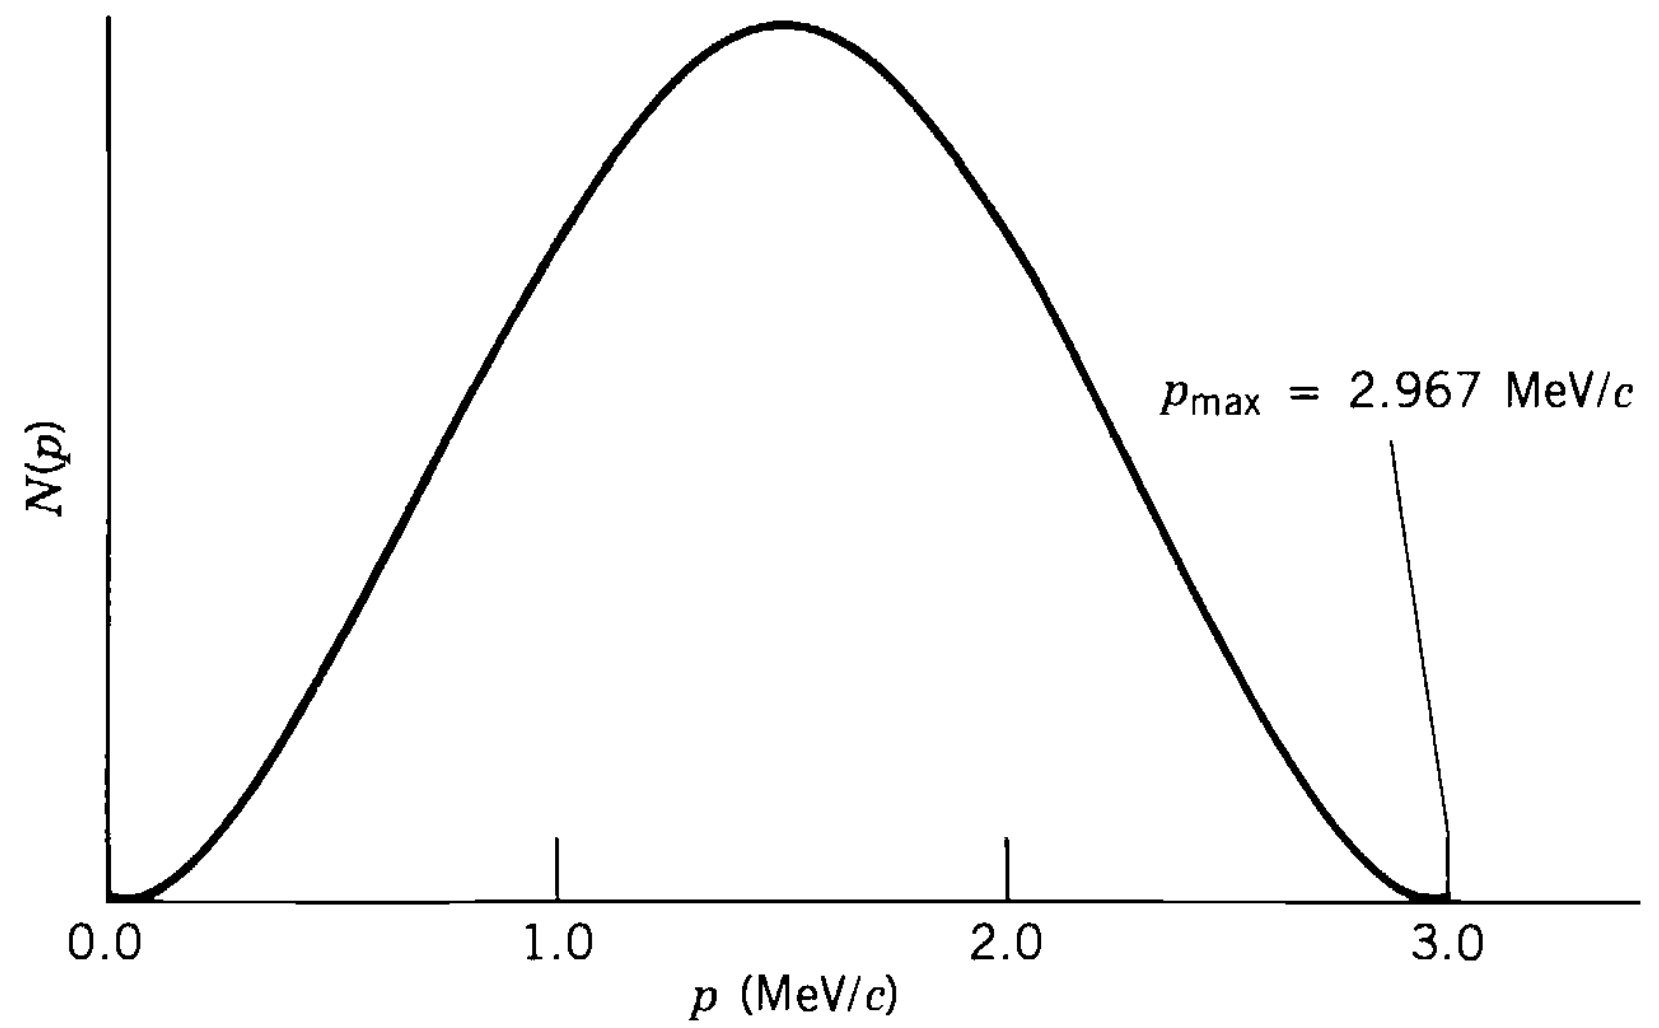
\includegraphics[width=0.45\textwidth]{beta-mom.png}
	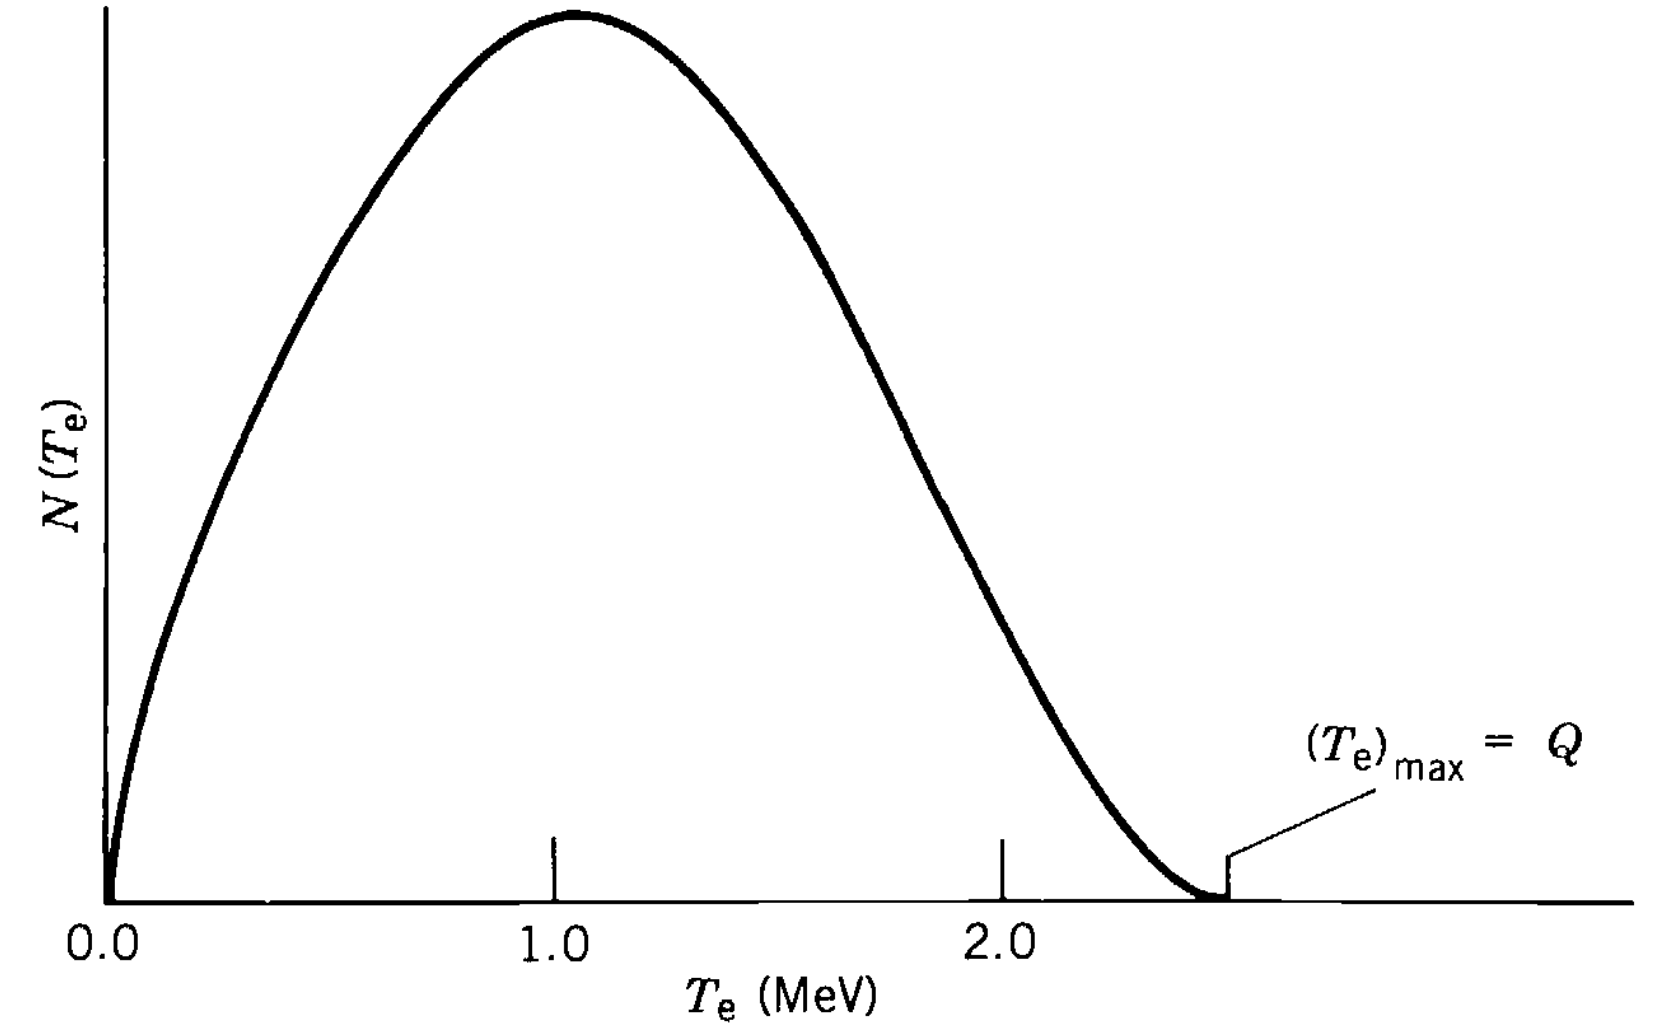
\includegraphics[width=0.45\textwidth]{beta-kin.png}
	\caption{Momentum and energy distributions of electrons from $ \beta $ decay.}
	\label{beta-spectrum}
\end{figure}

Analizzando gli spettri energetici, inoltre, si trova che $ Q_{\beta} \approx Q $: ciò implica che il neutrino ha massa estremamente piccola. Inoltre, per conservazione del momento angolare, è necessario che esso abbia spin semi-intero: considerando ad esempio il decadimento $ \ch{^{14}_6 C} \rightarrow \ch{^{14}_7 N} + e^- + \bar{\nu}_e $, se il neutrino non avesse spin semi-intero si avrebbe una violazione della conservazione di $ I $, dato che entrambi i nuclidi hanno $ I $ intero e l'elettrone ha $ s = \frac{1}{2} $.

\subsection{Teoria di Fermi}\label{fermi-th-sec}

A partire dall'ipotesi del neutrino di Pauli (1931), nel 1934 Fermi formulò una teoria per descrivere il decadimento $ \beta $; in particolare, si fanno le seguenti assunzioni:
\begin{enumerate}
	\item si trascura l'interazione coulombiana tra elettrone e nucleo (valido per nuclei con $ Z < 10 $);
	\item si trascura il nuclear recoil (valido poiché $ m_e \ll M_{\text{nucleo}} $);
	\item si considera il neutrino massless;
	\item si considerano equiprobabili tutte le possibili partizioni dell'energia tra elettrone e neutrino.
\end{enumerate}
Da questi assunti, si ricava che il bilancio energetico del processo è dato da:
\begin{equation}
	E = E_e + E_{\nu} = T_e + m_e c^2 + c p_{\nu}
	\label{eq:2.23}
\end{equation}
dalla quale si trova che $ T_e^{\text{max}} = E - m_e c^2 = Q $. La legge fondamentale postulata da Fermi per descrivere il decadimento è la \textit{golden rule}:
\begin{equation}
	\lambda = \frac{2\pi}{\hbar} \abs{M}^2 \frac{dn}{dE}
	\label{eq:2.24}
\end{equation}
Il termine $ \frac{dn}{dE} $ è dovuto alla natura dello spazio delle fasi e rappresenta la densità degli stati finali possibili per il decadimento ($ dn $ sono gli stati finali energeticamente possibili tra $ E $ ed $ E + dE $), mentre $ \abs{M}^2 $ è detto elemento di matrice dell'operatore di transizione $ \hat{H} $ e stima la probabilità di overlap tra lo stato iniziale e quello finale del sistema:
\begin{equation}
	M \defeq \braket{\psi_{\text{f}} | \hat{H} | \psi_{\text{i}}} = \int_V d^3\ve{x}\, \psi^*_{\text{f}}(\ve{x}) \hat{H} \psi_{\text{i}}(\ve{x})
	\label{eq:2.25}
\end{equation}
dove $ \psi_{\text{f}} = \psi_{\text{Y}} \psi_e \psi_{\nu} $. Il calcolo dell'elemento di matrice è estremamente complicato, specialmente per la difficoltà di calcolare le funzioni d'onda nucleari.\\
Si supponga che nel decadimento l'elettrone venga emesso con momento $ \ve{p}_e $: dato che la direzione di emssione è ininfluente con le semplificazioni fatte, ricordando che l'elemento di volume minimo dello spazio delle fasi è $ h^3 $ si trova che, confinando il sistema in un volume $ V $ (formalità solo per normalizzare le funzioni d'onda), il numero $ dn_e $ di stati elettronici finali con momento tra $ p_e $ e $ p_e + dp_e $ è:
\begin{equation}
	dn_e = \frac{4\pi p_e^2 V}{h^3} dp_e
	\label{eq:2.26}
\end{equation}
Ragionando analogamente per il neutrino, si trova che il numero totale di stati $ dn $ in funzione dei momenti $ p_e $ e $ p_{\nu} $ è:
\begin{equation}
	dn = dn_e dn_{\nu} = \left( \frac{4\pi V}{h^3} \right)^2 p_e^2 dp_e p_{\nu}^2 dp_{\nu}
	\label{eq:2.27}
\end{equation}
Ricordando il vincolo $ E = E_e + E_{\nu} $, si ha che $ cp_{\nu} = E - E_e $ e, fissata $ E_e $, $ dp_{\nu} = \frac{dE}{c} $, quindi:
\begin{equation}
	\frac{dn}{dE} = \left( \frac{4\pi V}{h^3} \right)^2 \frac{1}{c^3} (E - E_e)^2 p_e^2 dp_e
	\label{eq:2.28}
\end{equation}
Si assume $ \abs{M}^2 $ indipendente da $ p_e $, me è necessario considerare una correzione dovuta all'interazione coulombiana a cui è soggetto l'elettrone/positrone: come si vede in Fig. \ref{beta-coul}, la repulsione dei positroni porta ad averne meno ad energie basse, mentre l'attrazione degli elettroni diminuisce quelli ad alta energia. La correzione analitica è data dalla \textit{funzione di Fermi}:
\begin{equation}
	F(Z,E_e) \approx \frac{2\pi \eta}{1 - e^{-2\pi \eta}}
	\label{eq:2.29}
\end{equation}
dove $ \eta $ è il \textit{parametro di Sommerfeld}, che per $ e^{\pm} $ è definito come:
\begin{equation}
	\eta \equiv \mp \frac{Ze^2}{\hbar v_e}
	\label{eq:2.30}
\end{equation}
con $ v_e $ velocità asintotica dell'elettrone/positrone. Per $ \eta \ll 1 $ si ha $ F(Z,E_e) \approx 1 $.\\
È dunque possibile esprimere la probabilità di disintegrazione differenziale grazie alla golden rule:
\begin{equation}
	d\lambda(p_e) = C \abs{M}^2 F(Z,E_e) (E - E_e)^2 p_e^2 dp_e
	\label{eq:2.31}
\end{equation}
con $ C $ una costante. È stato possibile eliminare la dipendenza dal neutrino poiché la sua energia è fissata da quella dell'elettrone/positrone.

\begin{figure}[b!]
	\centering
	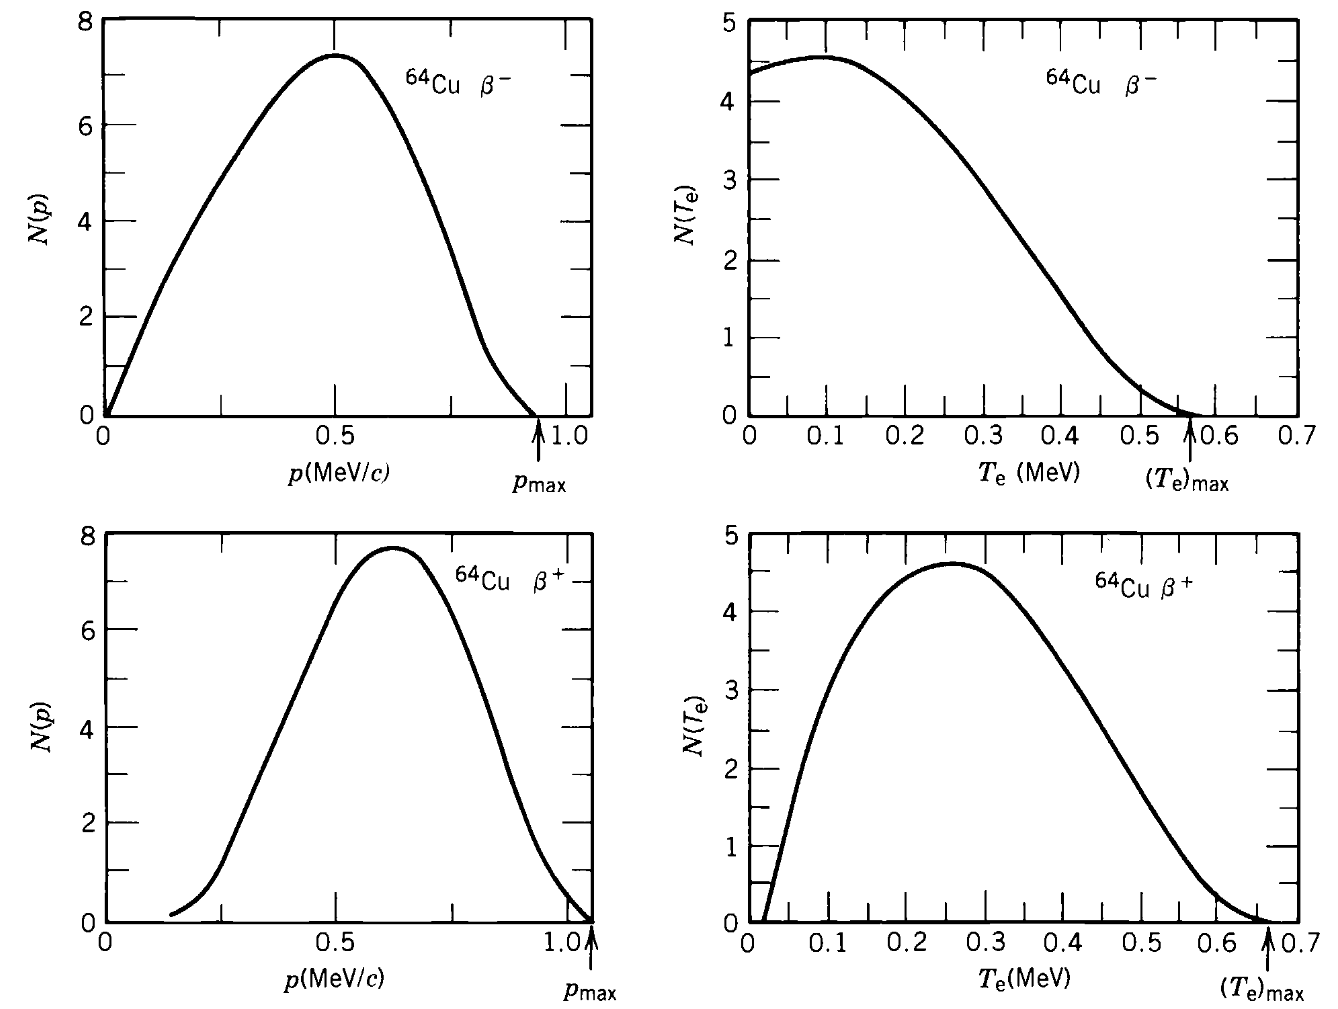
\includegraphics[width=0.70\textwidth]{beta-coul.png}
	\caption{Momentum and kinetic energy spectra of electrons and positrons emitted from $ \ch{^{64}_{29}Cu} $ decay.}
	\label{beta-coul}
\end{figure}

È possibile ottenere $ \lambda $ integrando su $ [0, p_e^{\text{max}}] $, dove il momento elettronico massimo si ottiene ponendo nullo quello neutrinico, ovvero $ p_e^{\text{max}} = \frac{1}{c} \sqrt{E^2 - m_e^2 c^4} $.\\
È inoltre utile definire la \textit{funzione di Fermi-Kurie}:
\begin{equation}
	K(E_e) \defeq \sqrt{\frac{\frac{d\lambda(p_e)}{dp_e}}{p_e^2 F(Z,E_e)}} \propto E - E_e
	\label{eq:2.32}
\end{equation}
Dall'analisi del Fermi-Kurie plot è possibile ottenere informazioni sulla massa del neutrino: infatti, con metodi di regressione lineare è possibile individuare quando $ E - E_e $ si annulla con una buona precisione, mentre misurare in maniera diretta il valore di energia massimo sarebbe complicato.

\subsubsection{Massa del neutrino}

Nel caso in cui si consideri un neutrino di massa non-nulla $ m_{\nu} $, la sua energia va calcolata come:
\begin{equation}
	E_{\nu} = \sqrt{p_{\nu}^2 c^2 + m_{\nu}^2 c^4}
	\label{eq:2.33}
\end{equation}
Differenziando $ p_{\nu}^2 c^2 = (E - E_e)^2 - m_{\nu}^2 c^4 $ e moltiplicando per $ p_{\nu} $, si trova:
\begin{equation}
	p_{\nu}^2 dp_{\nu} = \frac{1}{c^3} \sqrt{(E - E_e)^2 - m_{\nu}^2 c^4} (E - E_e) dE
	\label{eq:2.34}
\end{equation}
Dall'Eq. \ref{eq:2.27}-\ref{eq:2.31}, si trova quindi l'equazione corretta:
\begin{equation}
	d\lambda(p_e) = C \abs{M}^2 F(Z,E_e) \sqrt{(E - E_e)^2 - m_{\nu}^2 c^4} (E - E_e) dE
	\label{eq:2.35}
\end{equation}
Di conseguenza, varia l'andamento di $ K(E_e) $: in particolare, in prossimità di $ E - E_e = 0 $ l'andamento non sarà lineare ma radicale, e diversi valori di $ m_{\nu} $ determineranno end-point energies diverse.\\
Questo è uno dei metodi sperimentali più usati per misurare la massa del neutrino, sebbene nel tempo studi sul decadimento del trizio abbiano portato a risultati diversi: gli ultimi dati dell'esperimento Katrin (Karlsuhe, 2022) pongono $ m_{\nu} < 0.8 \ev $.

\section{Decadimento \texorpdfstring{$ \gamma $}{TEXT}}

Il decadimento $ \gamma $ è un processo elettromagnetico in cui il nucleo diminuisce la sua excitation energy senza variare il numero di protoni e neutroni. Questo decadimento avviene tramite l'emissione di fotoni, i bosoni massless e di spin 1 che mediano l'interazione elettromagnetica, i quali trasportano energie che vanno dai keV alle decine di MeV.\\
Oltre al decadimento $ \gamma $, ci sono altri due modi elettromagnetici di diseccitazione: la pair production, che avviene quando l'emissione di un fotone è proibita dalle selection rules e $ \Delta E > 2m_e = 1.022 \mev $, e l'electron conversion, in cui l'energia da emettere viene ceduta ad un elettrone, il quale viene così emesso dall'atomo (tipicamente elettroni degli orbitali interni). Questi decay modes, però, sono poco probabili, per questo quando si parla di diseccitazione elettromagnetica ci si riferisce sostanzialmente al decadimento $ \gamma $.

\subsection{Caratteristiche del decadimento \texorpdfstring{$ \gamma $}{TEXT}}

Tipicamente il decadimento $ \gamma $ è il decay mode dominante negli stati nucleari eccitati: lo studio dei raggi $ \gamma $ emessi permette di inferire varie proprietà degli stati nucleari coinvolti, come ad esempio lo spin, la parità, il momento magnetico, la vita media etc.\\
Nello studio degli spettri $ \gamma $ bisogna ricordare che è sempre presente un fondo naturale, dovuto al fatto che gli elementi delle principali catene di decadimento (ad esempio quella del $ \ch{^{238}U} $), sebbene decadano $ \alpha $ e $ \beta $, possono venire prodotti non nel loro stato fondamentale ma in uno stato eccitato, dunque prima di proseguire la catena essi decadono $ \gamma $: anche le sorgenti $ \alpha $ e $ \beta $ emettono raggi $ \gamma $.\\
Dato un raggio $ \gamma $ di energia $ E $, ricordando che $ E = h \nu $ e $ \nu \lambda = c $, la sua lunghezza d'onda è:
\begin{equation}
	\lambda = \frac{hc}{E}
	\label{eq:2.36}
\end{equation}
Dunque, un raggio $ \gamma $ di energia $ 1\mev $ (tipico ordine di grandezza) ha una lunghezza d'onda di $ 1240\fm $, ben superiore alle dimensioni del nucleo atomico ($ 6\fm $ per $ A = 100 $).\\
Considerando invece uno stato nucleare eccitato di vita media $ \tau $, dal principio di Heisenberg si può definire la sua \textit{energy width} $ \Gamma $ come:
\begin{equation}
	\Gamma \approx \frac{\hbar}{\tau}
	\label{eq:2.37}
\end{equation}
Per uno stato di vita media $ \tau = 1 \,\text{ps} $ si ha $ \Gamma = 0.66 \cdot 10^{-3} \ev $, che è praticamente infinitesima e trascurabile poiché di vari ordini di grandezza inferiore all'attuale risoluzione dei rilevatori (detector al germanio ha una risoluzione di $ \sim 2\kev $).

\subsubsection{Nuclear recoil}

Si consideri un nuclide di massa $ m $ inizialmente a riposo in uno stato eccitato $ E_0 $: se esso decade in uno stato $ E_1 $ emettendo un raggio $ \gamma $, per la conservazione del momento e dell'energia esso dovrà avere una certa quantità di moto finale $ \ve{p}_r $ di rinculo, determinata da:
\begin{equation*}
	\begin{cases}
		E_0 = E_1 + E_{\gamma} + \frac{p_r^2}{2m} \\
		\ve{0} = \ve{p}_{\gamma} + \ve{p}_r
	\end{cases}
	\quad\Rightarrow\quad p_r = p_{\gamma} = \frac{E_{\gamma}}{c}
\end{equation*}
Il salto energetico $ \Delta E = E_0 - E_1 $ tra i due livelli è dunque:
\begin{equation}
	\Delta E = E_{\gamma} + \frac{E_{\gamma}^2}{2mc^2}
	\label{eq:2.38}
\end{equation}
Per ricavare l'energia del fotone, ricordando che $ \Delta E \ll mc^2 $:
\begin{equation}
	E_{\gamma} = mc^2 \left[ -1 \pm \sqrt{1 + \frac{2\Delta E}{mc^2}} \right] \approx \Delta E - \frac{\Delta E^2}{2mc^2}
	\label{eq:2.39}
\end{equation}
Dato che tipicamente $ \Delta E \sim 1\mev $ e $ mc^2 \sim A \cdot 10^3 \mev $, la correzione dovuta al nuclear recoil è dell'ordine di $ 10^{-5} \Delta E $, dunque in prima approssimazione si può affermare che l'energia del raggio $ \gamma $ è proprio la differenza di energia tra i due stati della transizione:
\begin{equation}
	E_{\gamma} = \Delta E
	\label{eq:2.40}
\end{equation}

\subsection{Emissione di raggi \texorpdfstring{$ \gamma $}{TEXT}}

Un nucleo eccitato emette fotoni quando l'excitation energy non è sufficiente a separare un nucleone dal nucleo (tipicamente servono $ \sim 8\mev $), dunque l'unico modo per diseccitarsi è emettere un fotone (quanto d'energia). Inoltre, ciò può avvenire anche per energie superiori alla soglia di separazione, nel caso in cui l'emissione di nucleone fosse vietata dalle regole di conservazione di parità e/o momento angolare.\\
Dallo studio del pattern di decadimento $ \gamma $ si possono ricavare subito informazioni sulla struttura del nucleo: un pattern regolare indica la presenza di una rotational band, ovvero un nucleo deformato, mentre un pattern irregolare può indicare un nucleo sferico.\\
Il fatto che il nucleo si disecciti tramite emissione di radiazione elettromagnetica si può capire dal fatto che il nucleo è un insieme di cariche che generano un campo elettromagnetico. Si ricordi che la radiazione elettromagnetica può essere generata da una carica oscillante, nel qual caso si parla di \textit{radiazione elettrica} E, o da una corrente/momento magnetico variabile nel tempo, che genera una \textit{radiazione magnetica} M. Inoltre, un campo elettromagnetico variabile generato da cariche e correnti dipendenti dal tempo può essere espresso tramite uno sviluppo in serie di multipoli, ciascuno caratterizzato da una distribuzione angolare di radiazione emessa, che quantisticamente corrispondono ai diversi valori di momento angolare trasportati dal fotone. Dunque, nella descrizione di onde elettromagnetiche, si parla di radiazione di \textit{multipolarità} $ \sigma L $, dove $ \sigma $ può essere E o M, ovvero la natura della radiazione, ed $ L $ è l'ordine di multipolo, ovvero il numero quantico di momento angolare del fotone.\\
A livello nucleare, le varie multipolarità sono dovute a differenti oscillazioni del fluido nucleare: le multipolarità $ \text{E}L $ sono dovute ad una redistribuzione della carica elettrica nel nucleo, mentre quelle $ \text{M}L $ ad una redistribuzione degli spin o dei momenti angolari orbitali dei nucleoni.

\subsubsection{Trattazione semiclassica}

Per studiare la radiazione $ \gamma $ emessa da un nuclide è possibile applicare l'approccio semiclassico, che prevede il calcolo della potenza emessa dai vari ordini multipolari in forma di onde elettromagnetiche: la limitazione di questo approccio è che è valido solo nella \textit{zona di radiazione}, ovvero sviluppando in serie il campo elettromagnetiche ad una distanza molto grande rispetto alle dimensioni della sorgente e alla lunghezza d'onda della radiazione; questa condizione però è sicuramente verificata nel caso del decadimento $ \gamma $. Per una descrizione a qualsiasi distanza è necessario un trattamento completamente quanto-meccanico.\\
In generale, la potenza media (mediata su tutte le direzioni, ovvero su $ \mathbb{S}^2 $) irradiata ad un ordine multipolare $ \sigma L $ è:
\begin{equation}
	P(\sigma L) = \frac{2c}{\epsilon_0} \frac{L + 1}{L [(2L + 1)!!]^2} \left( \frac{\omega}{c} \right)^{2L + 2} \abs{\mathcal{M}(\sigma L)}^2
	\label{eq:2.41}
\end{equation}
dove $ \mathcal{M}(\sigma L) $ è l'elemento di matrice che connette lo stato iniziale a quello finale e che dunque dà la dipendenza dalla struttura nucleare.\\
Per quanto riguarda la distribuzione angolare della radiazione ad un ordine multipolare $ \sigma L $, essa è determinata dal polinomio di Legendre $ P_{2L}(\cos \theta) $: questo rende possibie la determinazione dell'ordine di multipolarità studiando la distribuzione angolare della radiazione. Bisogna inoltre notare che la radiazione elettrica e quella magnetica hanno polarità opposte:
\begin{equation}
	\pi(\text{E}L) = (-1)^{L} \qquad \pi(\text{M}L) = (-1)^{L + 1}
	\label{eq:2.42}
\end{equation}
Ad esempio, la radiazione da dipolo elettrico E1 sarà caratterizzata da:
\begin{equation*}
	P(\text{E}1) = \frac{1}{12\pi \epsilon_0} \frac{\omega^4}{c^3} d^2 \qquad \pi(\text{E}1) = -1
\end{equation*}
dove $ \ve{d} \defeq q\ve{r} $, $ \ve{r} $ vettore di separazione tra le due cariche $ \pm q $. Si vede la parità negativa dal fatto che sotto operatore di parità $ \ve{r} \mapsto -\ve{r} $, dunque $ \ve{d} \mapsto -\ve{d} $.\\
Prendendo invece un dipolo magnetico M1:
\begin{equation*}
	P(\text{M}1) = \frac{1}{12\pi \epsilon_0} \frac{\omega^4}{c^5} \mu^2
\end{equation*}
dove $ \ve{\mu} \defeq q \ve{r}\times\ve{v} $, $ \ve{r} $ posizione e $ \ve{v} $ velocità della carica $ q $ in moto. Sotto operatore di parità $ \ve{r} \mapsto -\ve{r} $ e $ \ve{v} \mapsto -\ve{v} $, dunque $ \ve{\mu} $ rimane invariato.

\subsubsection{Momento angolare}

Dato che il fotone è un bosone di spin 1, esso può sottrarre unità di momento angolare al nucleo in base alla multipolarità della transizione. Dati gli stati iniziale e finale del nuclide, di rispettivo momento angolare $ I_{\text{i}} $ e $ I_{\text{f}} $, dalla conservazione del momento angolare si ottiene la selection rule per il momento angolare $ L $ del raggio $ \gamma $:
\begin{equation}
	\abs{I_{\text{i}} - I_{\text{f}}} \le L \le I_{\text{i}} + I_{\text{f}}
	\label{eq:2.43}
\end{equation}
Dato lo spin 1 del fotone, si ha l'ulteriore vincolo $ L \ge 1 $: di conseguenza, il decadimento $ \gamma $ è proibito per transizioni del tipo $ 0^{\pm} \rightarrow 0^{\pm} $, per i quali sono permesse solo le internal conversions (emissione di un elettrone di conversione) o i decadimenti con più di un fotone (estremamente improbabile). Infatti, la multipolarità E0 (di monopolo) corrisponde ad una distribuzione di carica statica invariante nel tempo, dunque non produce radiazione, mentre M0 non esiste proprio data l'assenza sperimentale di monopoli magnetici.\\
Alcuni nuclidi, come ad esempio $ \ch{^{68}Ni} $, $ \ch{^{90}Zr} $ e $ \ch{^{186}Pb} $, hanno come primo stato eccitato uno stato $ 0^+ $: lo studio di come questi stati decadano al ground state $ 0^+ $ è importante per capire come le diverse forme della superficie nucleare coesistano assieme ad energie simili (dipende da come i nucleoni interagiscono tra loro).

\subsection{Probabilità di transizione}

Data una transizione $ \gamma $ di multipolarità $ \sigma L $, mediata da un fotone di frequenza angolare $ \omega $, si trova la probabilità di transizione come:
\begin{equation}
	T(\sigma L) \equiv \frac{P(\sigma L)}{\hbar \omega} = \frac{2}{\epsilon_0 \hbar} \frac{L + 1}{L [(2L + 1)!!]^2} \left( \frac{\omega}{c} \right)^{2L + 1} B(\sigma L)
	\label{eq:2.44}
\end{equation}
dove si definisce la \textit{probabilità di transizione ridotta} $ B(\sigma L) = \abs{\mathcal{M}_{\text{if}}(\sigma L)}^2 $, indipendente dall'energia di transizione (normalizzato rispetto ad essa) ma dipendente dagli elementi di matrice degli operatori di multipolo tra lo stato iniziale e finale, che è difficile da calcolare dato che non si conoscono con esattezza le funzioni d'onda nucleari.

\subsubsection{Stime di Weisskopf}

Per rendere possibile lo svolgimento analitico del calcolo di $ B(\sigma L) $, si considera il modello a shell (a particelle indipendenti) e si assume che la transizione sia dovuta ad un singolo protone che passa da una shell all'altra: dopo alcune ragionevoli semplificazioni, si ottengono le cosiddette \textit{stime di Weisskopf} per $ B(\sigma L) $.\\
Assumendo una transizione $ \sigma L $ da uno stato eccitato di un nuclide di numero di massa $ A $ al suo ground state:
\begin{equation}
	B(\text{E}L; I_{\text{i}} \rightarrow I_{\text{gs}}) = \frac{(1.2)^{2L}}{4\pi} \left( \frac{3}{L + 3} \right)^2 A^{2L/3} \,e^2 (\text{fm})^{2L}\\
	\label{eq:2.45}
\end{equation}
\begin{equation}
	B(\text{M}L; I_{\text{i}} \rightarrow I_{\text{gs}}) = \frac{10}{\pi} (1.2)^{2L - 2} \left( \frac{3}{L + 3} \right)^2 A^{(2L - 2)/3} \,\mu_N^2 (\text{fm})^{2L - 2}
	\label{eq:2.46}
\end{equation}
Si vede dunque che le probabilità ridotte per transizioni elettriche possono essere espresse in $ e^2 \text{barn}^L $, mentre per transizioni magnetiche in $ \mu_N^2 \text{barn}^{L - 1} $. Queste dipendono dalla multipolarità della transizione, ma non dalla sua energia: la dipendenza da $ E_{\gamma} $ è contenuta nel fattore in Eq. \ref{eq:2.44}. Ad esempio, si trova che $ T(\text{E}1) = 1.0 \cdot 10^{14} A^{2/3} E_{\gamma}^3 $, $ T(\text{E}2) = 7.3 \cdot 10^7 A^{4/3} E_{\gamma}^5 $, $ \dots $, $ T(\text{M}1) = 3.1 \cdot 10^{13} E_{\gamma}^3 $, $ T(\text{M}2) = 2.2 \cdot 10^7 A^{2/3} E_{\gamma}^5 $, $ \dots $\\
Si trova che, in generale, confrontando tra transizioni dello stesso tipo (E o M), la probabilità di transizione $ T $ diminuisce all'aumentare di $ L $, anche di 4 ordini di grandezza, mentre a parità di ordine di multipolo sono predominanti le transizioni elettriche, di 2 o 3 ordini di grandezza.\\
$ T(\sigma L) $ è espresso in $ \text{s}^{-1} $ e può essere identificato nella costante di decadimento $ \lambda $ della transizioni $ \sigma L $; di conseguenza, si ha che la vita media dello stato eccitato è $ \tau = \frac{1}{T(\sigma L)} $: queste variano da $ 10^{-15}\,\text{s} $ a svariati anni, tempi estremamente grandi rispetto al tempo medio in cui un nucleone attraversa il nucleo ($ \sim 10^{-22}\,\text{s} $). Inoltre, se le uniche transizioni ammesse dalle selection rule tra due stati sono ad alto ordine multipolare, la vita media può essere talmente lunga (giorni o anni, mentre tipicamente è $ \sim 1\text{ps} $) che si parla di \textit{stati isomerici}.\\
Il confronto dei valori teorici di Weisskopf con i dati sperimentali è molto importante: una probabilità di transizione molto pià piccola del previsto può indicare che i due stati nucleari iniziale e finale sono molto diversi tra loro, mentre una probabilità molto più grande del previsto può equivalere al fatto che nella transizione sono coinvolti non uno a molti nucleoni. Il confronto avviene esprimendo le probabilità osservate sperimentalmente in Weisskopf units $ B_{\text{sp}} $, ovvero studiando il rapporto $ B(\sigma L) / B_{\text{sp}}(\sigma L) $: questo si attesta circa all'unità nell'intorno delle double shell closures, a riprova che le stime teoriche descrivono bene i nuclei caratterizzati dalle eccitazioni di nucleoni singoli, mentre può assumere valori anche di qualche centinaia per nuclei in cui si hanno stati collettivi, ad esempio quelli caratterizzati da stati vibrazionali di quadrupolo nei nuclidi sferici o nelle rotational bands dei nuclidi deformati.












\chapter{Radiazioni}
\pagestyle{body}
\selectlanguage{italian}

L'interazione delle radiazioni con il mezzo in cui si propagano dipende dalla natura delle particelle di cui esse sono composte:
\begin{itemize}
	\item particelle cariche, che hanno un'interazione continua con gli elettroni del mezzo a causa della forza coulombiana:
	\begin{itemize}
		\item particelle cariche pesanti (range tipico $ \sim 10^{-5} \m $);
		\item elettroni veloci (range tipico $ \sim 10^{-3} \m $);
	\end{itemize}
	\item particelle neutre, che invece non subiscono l'interazione coulombiana ma agiscono in maniera discreta, causando un grande scambio energetico per ogni singola interazione (spesso con i nuclei):
	\begin{itemize}
		\item raggi X e $ \gamma $ (range tipico $ 10^{-1} \m $);
		\item neutroni (range tipico $ 10^{-1} \m $).
	\end{itemize}
\end{itemize}
Per quanto riguarda i principali tipi di radiazioni, che rispecchiano ciascuna delle casistiche appena evidenziate:
\begin{enumerate}
	\item raggi $ \alpha $: percorrono qualche centimetro in aria, vengono arrestati da un foglio di carta;
	\item raggi $ \beta $: percorrono qualche metro in aria, vengono arrestati da qualche millimetro di alluminio;
	\item raggi $ \gamma $: a seconda dell'energia, percorrono fino a molte centinaia di metri in aria, vengono arrestati da notevoli spessori di cemento o piombo;
	\item neutroni: la penetrazione dipende dall'energia, vengono arrestati da notevoli spessori di cemento, acqua o paraffina.
\end{enumerate}

\section{Particelle cariche}

Il tipo di interazione dominante tra radiazione e materia sono le collisioni inelastiche con gli elettroni del mezzo: ciò induce vari fenomeni, principalmente l'eccitazione degli atomi, la loro ionizzazione, la fluorescenza e la fosforescenza del materiale (questi ultimi sono causati dal tempo di diseccitazione molto lento degli stati molecolari, che genera l'emissione di luce visibile).\\
Dato che le interazioni avvengono principalmente con gli elettroni atomici, si può calcolare il rapporto delle sezioni d'urto coulombiane:
\begin{equation}
	\frac{\sigma_{\text{nucl}}}{\sigma_{\text{atom}}} \sim \frac{\pi R^2}{\pi a_Z^2} \approx \frac{A^{2/3} \cdot 10^{-26} \,\text{cm}^2}{10^{-16} \,\text{cm}^2} = A^{2/3} \cdot 10^{-10}
	\label{eq:3.1}
\end{equation}
Il range tipico per questo rapporto è dunque tra $ 10^{-7} $ e $ 10^{-8} $.

\subsection{Scattering e straggling}

A livello cinematico, considerando una particella di massa $ m \gg m_e $ e velocità $ v_0 $ incidente su un elettrone a riposo:
\begin{equation*}
	\begin{cases}
		\frac{1}{2} m v_0^2 = \frac{1}{2} m v_f^2 + \frac{1}{2} m_e v_e^2 \\
		m v_0 = m v_f + m_e v_e
	\end{cases}
	\quad\Rightarrow\quad
	\begin{cases}
		v_f = \frac{m - m_e}{m + m_e} v_0 \\
		v_e = \frac{2m}{m + m_e} v_0
	\end{cases}
\end{equation*}
Dato che $ v_e \approx 2v_0 $, si ha che:
\begin{equation}
	K_e = 4 \frac{m_e}{m} K_0
	\label{eq:3.2}
\end{equation}
Se ad esempio si considera un protone ($ m_p \approx 2000 m_e $), si vede che $ \Delta K_p = \frac{1}{500} K_0 $, quindi in circa 500 collisione esso viene completamente arrestato: questo avviene in pochi micrometri di materiale.\\
Si vede dunque che c'è una perdita di energia nel corso di numerose interazioni: il processo è graduale. Inoltre, al diminuire dell'energia le particelle incidenti tendono a deviare sempre di più dal percorso rettilineo originario a causa degli scattering, andando a creare uno sciame di particelle: questo fenomeno, detto \textit{straggling}, è sia energetico che posizionale, in quanto ci sarà una regione del materiale nel quale è presente la concentrazione più alta di particelle di radiazione.\\
La proiezione della traiettoria di una particella lungo la direzione di propagazione iniziale è detta \textit{range} ed ha un comportamento stocastico: il range sarà distribuito (diffuso) sia posizionalmente (dipendenza dal materiale) che energeticamente (dipendenza dalla particella), infatti si parla di range straggling. Quantitativamente, detto $ d\ve{s} $ il displacement tra uno scattering e l'altro e $ \theta_s $ l'angolo tra $ d\ve{s} $ e la direzione iniziale di propagazione, si definisce il range come:
\begin{equation}
	R(E) \defeq \int ds \braket{\cos \theta_s} = \int_0^E dE \left( \frac{dE}{ds} \right)^{-1} \braket{\cos \theta_s}
	\label{eq:}
\end{equation}
dove $ \frac{dE}{ds} $ è detto \textit{stopping power} ed esprime la perdita di energia per unità di lunghezza percorsa. Si vede subito che il range è più piccolo dell'effettiva traiettoria percorsa: $ \int ds \ge R(E) $.

\subsection{Modello fenomenologico}

È possibile formulare dei modelli fenomenologici per esprimere lo stopping power in funzione delle caratteristiche della particella e del materiale.\\
Un primo modello fu proposto da Lindhardt, che con la sua teoria dell'elettrone descrisse la perdita di energia causata dalla ionizzazione del materiale:
\begin{equation}
	- \frac{1}{\rho} \frac{dE}{ds} \approx \frac{4\pi Z_p^2 e^4}{m_e v^2} Z_t \frac{1}{2} \ln \left[ \frac{2m_e v^2}{I} \right]
	\label{eq:3.4}
\end{equation}
dove $ \rho $ è la densità atomica del materiale, $ Z_t $ il numero atomico degli atomi target, $ Z_p $ quello della particella incidente, $ v $ la sua velocità e $ I $ è la cosiddetta \textit{ionizing energy}, un parametro empirico che rappresenta l'energia d'eccitazione media degli elettroni nel materiale. Si vede che il fattore dominante è il primo, mentre il logaritmo diventa importante per alte velocità.\\
Un modello che descrive meglio le particelle massive ($ m \gg m_e $) anche in regime relativistico è quello dato dall'\textit{equazione di Bethe-Bloch}, che esprime l'average energy loss:
\begin{equation}
	-\frac{1}{\rho} \frac{dE}{ds} \approx 0.1535 \frac{Z_p^2}{\beta^2} \frac{Z_t}{A_t} \left[ 2 \ln \left( \frac{2m_e c^2}{I (1 - \beta^2)} \right) - 2\beta^2 \right] \text{MeV} \text{cm}^2 \text{g}^{-1}
	\label{eq:3.5}
\end{equation}
Empiricamente, si trova:
\begin{equation}
	I = h \braket{\nu_e} =
	\begin{cases}
		(12 Z_t + 7) \ev & Z_t < 13 \\
		(9.76 Z_t + 58.8 Z_t^{-0.19}) \ev & Z_t \ge 13
	\end{cases}
	\label{eq:3.6}
\end{equation}
È importante ricordare gli andamenti dello stopping power in funzione dei vari parametri:
\begin{itemize}
	\item $ \sim \rho Z_t $, maggiore per materiali densi;
	\item $ \sim Z_p^2 $, maggiore per raggi di ioni pesanti;
	\item $ \sim v^{-2} $, maggiore per particelle lente.
\end{itemize}
In particolare, l'andamento $ \sim v^{-2} $ è equivalente a $ \sim K_0^{-1} $: la proporzionalità inversa all'energia della particella incidente è seguita sperimentalmente con buon accordo fino al minimo di ionizzazione del materiale, ovvero all'energia per cui c'è probabilità minore di interazione tra radiazione e mezzo (dunque minore stopping power). Per energie elevate, al limite relativistiche, i termini $ \beta^2 $ diventano dominanti; inoltre, è necessario apportare delle correzioni per considerare le perdite radiative da Bremsstrahlung ed eventuali effetti $ \rho $-dependent nei plasmi.\\
In Fig. \ref{silicon} è possibile osservare come, fissato il mezzo, lo stopping power aumenti come all'aumentare di $ Z_p $ e diminuisca all'aumentare di $ K_0 $; inoltre, si può vedere come gli ioni più pesanti, per raggiungere lo stesso range, necessitino di maggiore energia.

\begin{figure}[!b]
	\centering
	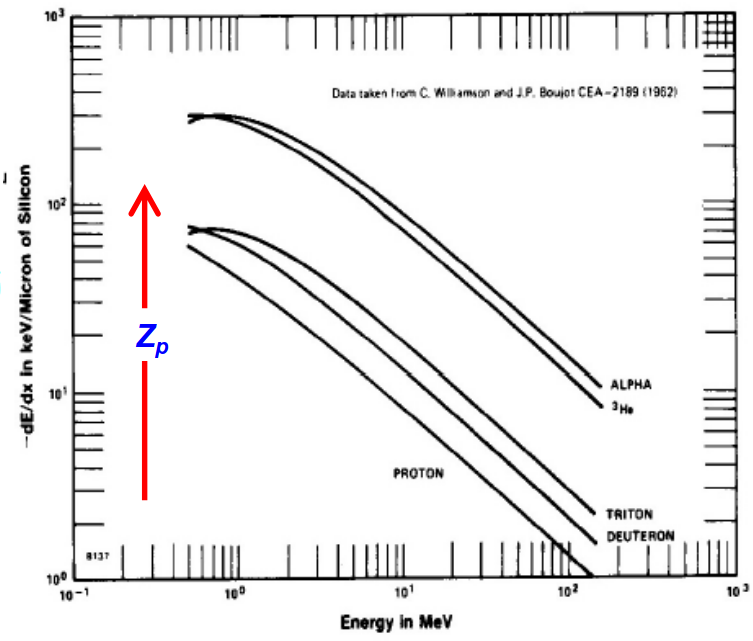
\includegraphics[width=0.45\textwidth]{silicon-sp.png}
	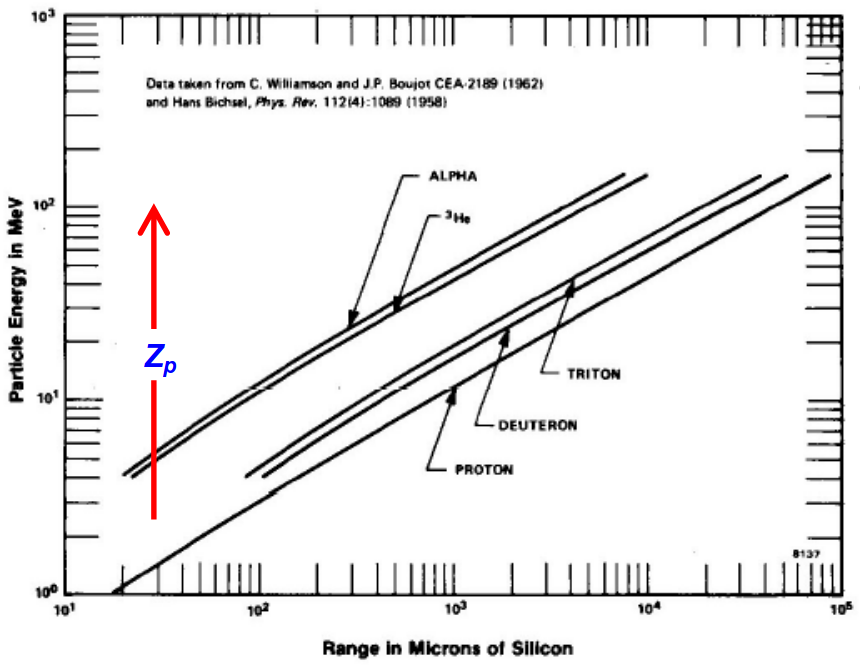
\includegraphics[width=0.495\textwidth]{silicon-r.png}
	\caption{Stopping power and range in Silicon.}
	\label{silicon}
\end{figure}

\paragraph{Particle identification}

Se si ha uno strumento in grado di misurare sia la perdita di energia di una particella carica che la sua energia totale\footnote{Un esempio potrebbe essere un rilevatore al silicio con due strati: uno sottile per misurare la perdita di energia ed uno spesso per fermare la particella, così da poter sommare le due rilevazioni ed ottenere l'energia totale.}, è possibile correlarle ed ottenere dei rami d'iperbole descritti da $ \frac{dE}{ds} E \propto Z_p^2 $. In questo modo si può distinguere tra i vari fasci di particelle ed identificarle, senza però poterne estrarre le masse.

\paragraph{Bragg peak}

La graduale perdita di energia nel range è ciò che sta alla base delle tecniche di adroterapia, ovvero la cura di tumori tramite bombardamento con particelle cariche (soprattutto protoni). Per fare ciò, è necessario conoscere con elevata precisione la perdita di energia specifica (perdita di energia per unità di massa del target) ed il range: quando una particella carica attraversa il corpo umano, essa ionizza tutto il materiale che percorre.\\
Per avere la massima efficacia, sarebbe ideale che la maggior parte dell'energia venisse dissipata in un intervallo specifico del range, così da poter attaccare accuratamente il tumore, ma questo è proprio ciò che avviene: più spazio viene percorso, più la particella perde energia e, di conseguenza, rallenta, quindi la maggior parte dell'energia viene rilasciata alla fine del range, nel cosiddetto \textit{picco di Bragg}. In questo modo, si può regolare il fascio di ioni in modo da far rilasciare la maggior parte dell'energia nel punto in cui si trova la massa tumorale.\\
Per avere un metro di misura della perdita di energia specifica si definisce la dose assorbita $ \frac{dE}{dm} $, misurata in $ \text{gray} \equiv \text{J} / \text{kg} $, dove $ dE $ è l'energia rilasciata nella massa $ dm $ del mezzo dalla radiazione ionizzante. In Fig. \ref{bragg} è possibile vedere come la presenza del picco di Bragg renda i fasci di particelle cariche massive particolarmente efficaci nella cura di tumori.

\begin{figure}[!t]
	\centering
	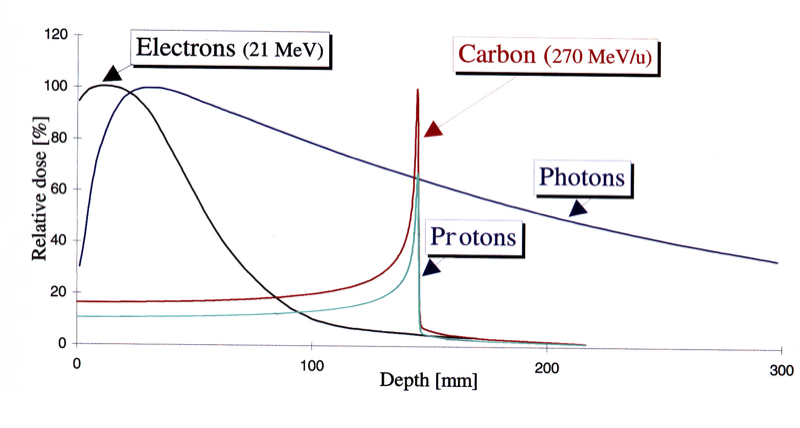
\includegraphics[width=1.00\textwidth]{bragg.png}
	\caption{Absorbed dose for different kinds of radiation.}
	\label{bragg}
\end{figure}

\section{Particelle neutre}

\subsection{Raggi \texorpdfstring{$ \gamma $}{TEXT}}

A differenza delle particelle cariche, i fotoni agiscono in maniera discreta col materiale e la ionizzazioni da essi causati avviene in regioni limitate del mezzo.\\
L'interazione dei fotoni col mezzo può avvenire in tre modi (vedere Fig. \ref{ph-i-p}):
\begin{enumerate}
	\item effetto fotoelettrico, dominante per $ E_{\gamma} < 500 \kev $;
	\item Compton scattering, dominante per $ 500 \kev \le E_{\gamma} \le 2 \mev $;
	\item pair production, dominante per $ E_{\gamma} > 2 \mev $.
\end{enumerate}

\begin{figure}[!b]
	\centering
	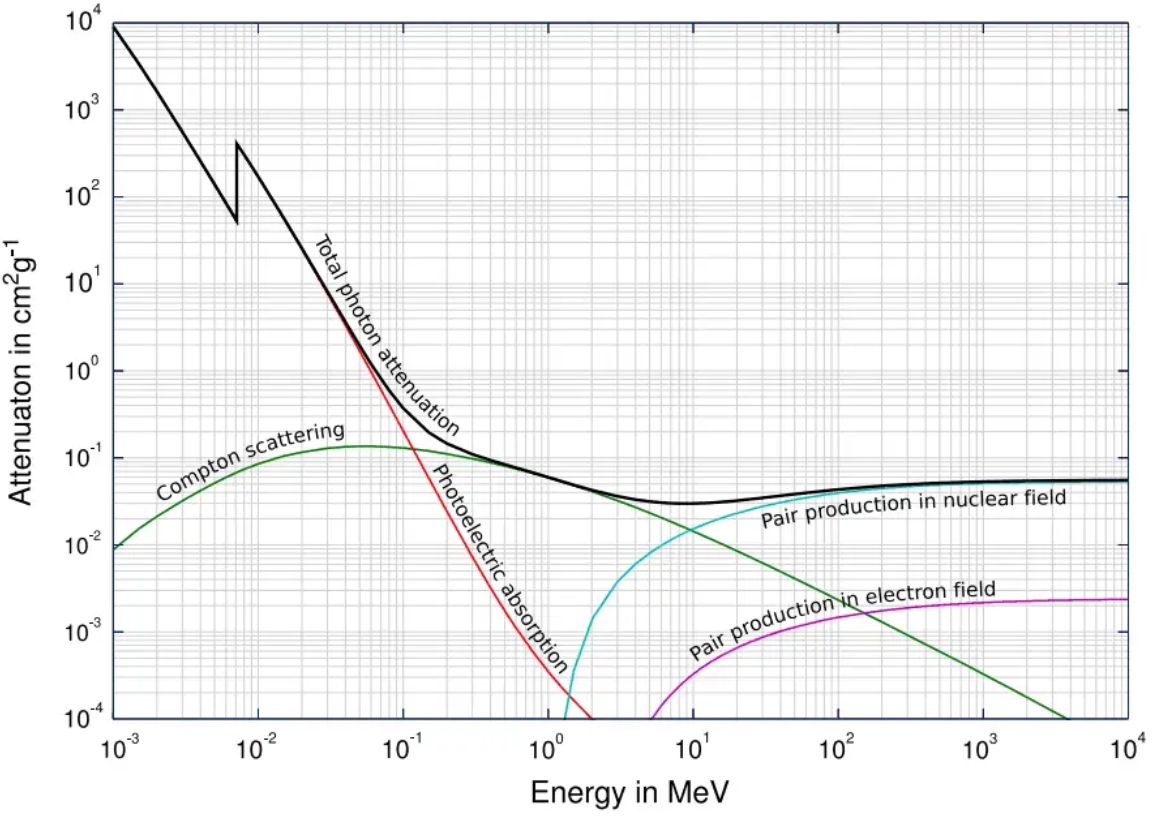
\includegraphics[width=0.70\textwidth]{lin-att-coeff.png}
	\caption{Linear attenuation coefficient for photon interaction.}
	\label{ph-i-p}
\end{figure}

È possibile definire una probabilità d'interazione per unità di lunghezza per ciascuno di questi processi, così da definire il \textit{coefficiente d'attenuazione lineare}:
\begin{equation}
	\mu = \sigma_{\text{ph}} + \sigma_{\text{C}} + \sigma_{\text{pp}}
	\label{eq:3.7}
\end{equation}
In questo modo, si può esplicitare la legge d'attenuazione per l'intensità del fascio di fotoni:
\begin{equation}
	I(x) = I_0 e^{-\mu x}
	\label{eq:3.8}
\end{equation}

\subsubsection{Effetto fotoelettrico}

Avviene quando un raggio $ \gamma $ colpisce un elettrone atomico: il fotone viene completamente assorbito e l'elettrone acquista abbastanza energia per fuoriuscire dall'atomo. In particolare, dato un fotone incidente di pulsazione $ \omega $:
\begin{equation}
	K_e = \hbar \omega - E_n
	\label{eq:3.9}
\end{equation}
dove $ E_n $ è la binding energy dell'elettrone, dipendente dal numero quantico principale e calcolabile con la legge di Moseley:
\begin{equation}
	E_n = Rhc \frac{(Z - \sigma)^2}{n^2}
	\label{eq:3.10}
\end{equation}
con $ Rhc = 13.6 \ev $ costante di Rydberg e $ \sigma $ un parametro dipendente dall'orbitale dell'elettrone (ad esempio $ \sigma_{\text{K}} \approx 3 $ e $ \sigma_{\text{L}} \approx 5 $).\\
Un fenomeno interessante è quello degli \textit{elettroni Auger}. Quando un materiale viene ionizzato, il vuoto creato dall'elettrone espulso viene colmato da un elettrone nella shell successiva: questo salto orbitale comporta l'emissione di un fotone, tipicamente un raggio X, e questa radiazione X è quella che viene tipicamente osservata; può capitare, però, che questo fotone, al posto di essere emesso, venga assorbito da un elettrone in una shell ancora più esterna, il quale viene così emesso dall'atomo: un elettrone di questo tipo viene detto elettrone Auger.

\subsubsection{Compton scattering}

È lo scattering relativistico tra un fotone ed un elettrone. Assumendo l'elettrone inizialmente a riposo:
\begin{equation*}
	\ve{p}_e = \ve{p}_{\gamma} - \ve{p}_{\gamma'} \quad\Rightarrow\quad p_e^2 c^2 = E_{\gamma}^2 + E_{\gamma'}^2 - 2E_{\gamma} E_{\gamma'} \cos \theta
\end{equation*}
dove $ \theta $ è l'angolo tra la direzione incidente e la direzione finale del fotone. Dal bilancio energetico dello scattering $ E_{\gamma} + m_e c^2 = E_{\gamma'} + E_e $ si ottiene:
\begin{equation}
	E_{\gamma'} = \frac{E_{\gamma}}{1 + \frac{E_{\gamma}}{m_e c^2} (1 - \cos \theta)}
	\label{eq:3.11}
\end{equation}
Il fotone con lo scattering subisce anche una variazione di lunghezza d'onda:
\begin{equation}
	\Delta \lambda = \frac{h}{m_e c} (1 - \cos \theta)
	\label{eq:3.12}
\end{equation}
Dopo un numero di interazioni il fotone viene arrestato: l'ultima interazione è di tipo fotoelettrico.\\
Il Compton scattering è un fenomeno importante quando si costruiscono rilevatori di raggi $ \gamma $: infatti, esso può portare ad una fuoriuscita di fotoni dal rilevatore (se vengono scatterati a determinati angoli), dunque l'energia misurata è parziale e c'è la presenza di un fondo, detto fondo Compton, eliminabile con delle tecniche note.

\subsubsection{Pair production}

È determinata dall'interazione tra un raggio $ \gamma $ ed il campo elettromagnetico presente nel materiale: l'interazione genera due particelle, un elettrone ed un positrone, e l'energia del fotone viene completamente convertita in questa coppia di particelle; successivamente, queste perdono energia all'interno del materiale. In particolare, dato che la massa dell'elettrone/positrone è $ m_ec^2 = 511\kev $, l'energia minima che deve possedere il raggio $ \gamma $ per far avvenire la pair production è $ E_{\text{min}} = 1.022\mev $.\\
Dirac formulò una teoria per spiegare la pair production: il mondo è composto da particelle normali con energia positiva $ E \ge m c^2 > 0 $, mentre esiste il cosiddetto \textit{Fermi sea} composto di particelle con energia negativa $ E \le - m c^2 < 0 $. L'interazione elettromagnetica può far transizionare una particella dal Fermi sea al mondo normale, riempiendo il gap energetico di $ \Delta E = 2mc^2 $: il buco lasciato nel Fermi sea è la sua corrispettiva antiparticella.\\
Le prime osservazioni del processo di pair production avvennero nelle camere a bolle: quando un fotone energetico interagisce con un atomo, può avvenire la reazione $ \gamma \rightarrow e^- + e^+ $, eventualmente espellendo anche un ulteriore elettrone dall'atomo. Applicando un campo magnetico è possibile poi studiare il momento e la carica delle particelle così prodotte.

\subsubsection{Interazioni nucleari}

Per raggi $ \gamma $ particolarmente energetici ($ E_{\gamma} \gtrsim 8\mev $) sono possibili anche interazioni a livello nucleare, sebbene meno probabili. Un raggio $ \gamma $ incidente può indurre reazioni all'interno del nucleo, a seguito delle quali possono essere emesse particelle secondarie ad alta energie e/o una sequenza di raggi $ \gamma $ ad energia minore.

\subsection{Neutroni}

A differenza dei fotoni, i neutroni hanno una massa ed è necessario distinguere tra vari range energetici, poiché i processi d'interazione sono molto diversi, sebbene tutti a livello nucleare. Dato che l'interazione nucleare ha un raggio d'azione estremamente ridotto, comparabile al raggio nucleare $ \sim 10^{-15} \m $, i neutroni hanno una bassa probabilità d'interazione: ciò risulta in un minore stopping power ed un maggiore range. Si ricordi inoltre che i neutroni nel nucleo, essendo in stati legati, possono essere stabili, mentre quelli liberi decadono con una vita media di $ 14.76\,\text{min} $.\\
L'interazione con neutroni ha una probabilità che è circa $ 10^{-6} $ volte quella dell'interazione con particelle cariche; in base all'energia (cinetica) $ E_n $ iniziale del neutrone sono possibili diverse interazioni:
\begin{enumerate}
	\item $ E_n \sim 25 \,\text{meV} $: diffusione termica lenta, cattura neutronica (nucleo cattura il neutrone e decade $ \gamma $);
	\item $ E_n < 10 \mev $: scattering elastico (fino alla termalizzazione), cattura neutronica, eccitazione nucleare;
	\item $ E_n > 10 \mev $: scattering elastico ed inelastico, reazioni nucleari (con produzione di particelle cariche secondarie).
\end{enumerate}
I rilevatori di neutroni non rilevano direttamente i neutroni, bensì la radiazione e le particelle secondarie prodotte dai processi nucleari, ad esempio raggi $ \gamma $, particelle cariche ($ p^+ $, $ \alpha $ etc.), altri neutroni, prodotti di fissione e, per neutroni altamente energetici ($ E_n > 150\mev $), prodotti di spallazione: quest'ultimi sono particolarmente pericolosi perché la spallazione può dar luogo ad uno shower di particelle secondarie estremamente dannose per l'organismo.\\
Come si può vedere in Fig. \ref{n-cross-sec}, fino a $ 10\mev $ la cross-section d'interazione con la materia scala come l'inverso della velocità (ovvero come $ E_n^{-1/2} $), mentre per alte energie sono presenti dei fenomeni di risonanza dovute al fatto che il neutrone può interagire con stati nucleari con funzioni d'onda compatibili.

\begin{figure}[!t]
	\centering
	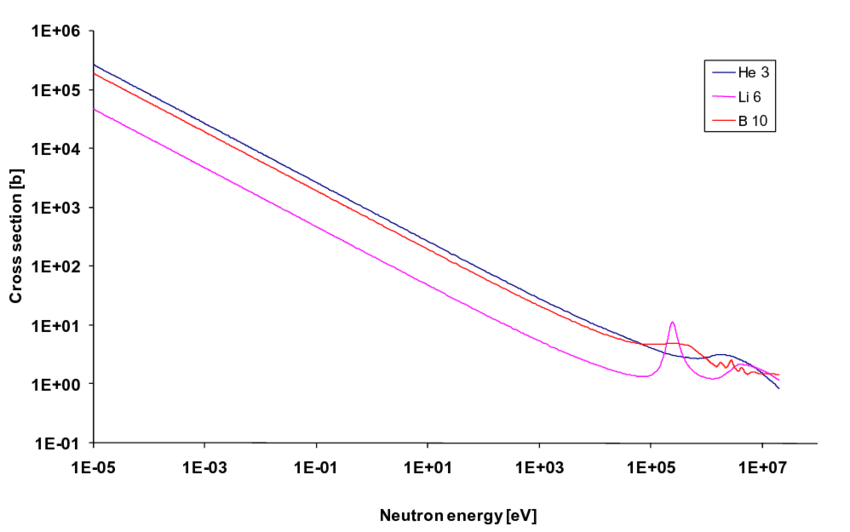
\includegraphics[width=0.60\textwidth]{n-cross-sec.png}
	\caption{Cross-section as a function of neutron energy.}
	\label{n-cross-sec}
\end{figure}

\subsubsection{Neutron detection}

La rilevazione di neutroni avviene tramite la rilevazione diretta delle particelle secondarie prodotte dalle interazioni dei neutroni con la materia. Le cross-sections di tali interazioni sono utili solo per neutroni termici lenti, dunque è necessario un moderatore che, tramite scattering, termalizzi i neutroni: il miglior moderatore è l'idrogeno, poiché con un singolo scattering può assorbire quasi tutta l'energia del neutrone. Infatti, dato lo scattering tra un neutrone di energia $ E_n $ ed un nucleo $ ^A_Z\text{X} $, detto $ \theta $ l'angolo tra la direzione incidente e la direzione risultante del neutrone, si ha che:
\begin{equation*}
	E_n' = E_n \left[ 1 - \frac{2 m_n M_A}{(m_n + M_A)^2} (1 - \cos \theta) \right] \approx E_n \frac{A^2 + 2A \cos \theta + 1}{(A + 1)^2} \quad\Rightarrow\quad \left( \frac{A - 1}{A + 1} \right)^2 E_n \le E_n' \le E_n
\end{equation*}
Si trova dunque che l'average energy loss è in percentuale pari a:
\begin{equation}
	\bigg\langle \frac{\Delta E_n}{E_n} \bigg\rangle = \frac{2A}{(A + 1)^2}
	\label{eq:3.13}
\end{equation}
che è massima per $ A = 1 $.\\
Per quanto riguarda i neutroni lenti ($ E_n < 0.5 \ev $), lo scattering elastico non favorisce la rilevazione, poiché l'energia ceduta al nucleo è poca per essere rilevata. Sono invece preferibili le reazioni nucleari neutron-induced, le quali producono particelle secondarie ($ \gamma $, $ p^+ $, $ \alpha $ etc.) abbastanza energetiche da essere rilevate.



\chapter{Interazione tra Nucleoni}
\pagestyle{body}
\selectlanguage{italian}

\section{Interazioni nucleone-nucleone}

\subsection{Bosoni e fermioni}

Si ricordi che un generico operatore di momento angolare soddisfa la condizione di commutazione:
\begin{equation}
	[\hat{L}_i,\hat{L}_j] = i\hbar \sum_{k = 1}^{3} \epsilon_{ijk} \hat{L}_k
	\label{eq:4.1}
\end{equation}
Diagonalizzando $ \hat{L}^2 $ e $ \hat{L}_z $:
\begin{equation}
	\hat{L}^2 \ket{\psi} = \hbar \ell (\ell + 1) \ket{\psi}
	\label{eq:4.2}
\end{equation}
\begin{equation}
	\hat{L}_z \ket{\psi} = \hbar m \ket{\psi}
	\label{eq:4.3}
\end{equation}
con $ m = -\ell, \dots, \ell $. Il momento angolare può essere sia orbitale che di spin (intrinseco): questo permette di distinguere particelle fermioniche e bosoniche.\\
Le particelle con spin semi-intero sono dette \textit{fermioni}, quelle con spin intero \textit{bosoni}: in maniera grossolana, si può dire che i fermioni costituiscono la materia, mentre i bosoni mediano le interazioni, ma ci sono delle eccezioni. Una delle principali proprietà è che, in sistemi di particelle identiche, le funzioni d'onda bosoniche sono simmetriche per scambio di particelle, mentre quelle fermioniche sono antisimmetriche: una conseguenza importante è il \textit{principio di esclusione di Pauli}, il quale afferma che due fermioni identici non possono avere gli stessi numeri quantici (ovvero avere lo stesso stato).\\
Si ricordi che, in generale, quando due momenti angolari interagiscono, i numeri quantici si compongono secondo:
\begin{equation}
	\abs{\ell_1 - \ell_2} \le j \le \ell_1 + \ell_2
	\label{eq:4.4}
\end{equation}
Ad esempio, un sistema di due fermioni può avere spin 0 o 1.

\subsection{Caratteristiche dell'interazione}

Non si conosce molto bene l'interazione tra nucleoni. Dallo studio della binding energy (vedere Fig. \ref{bind-en}) si evince che la binding energy per nucleone ($ B(A,Z)/A $) satura a circa $ 8\mev $: questo è una conseguenza del fatto che l'interazione tra nucleoni è a corto range. Infatti, le interazioni a lungo range scalano come $ E \sim \frac{1}{2} A (A - 1) $, come avviene ad esempio per quella coulombiana, mentre le interazioni a corto range come $ E \sim A $, dato che sono le particelle immediatamente vicine interagiscono tra loro.\\
Una stima cruda del range dell'interazioni tra nucleoni è data dalle dimensioni della particella $ \alpha $, che ha un daimetro di circa $ 1.5\fm $: si evince che il range dell'interazioni è circa tra $ 1\fm $ e $ 2\fm $.\\
In maniera più precisa, si può determinare il range a partire dal mediatore dell'interazione: dato che durante un'interazione la particella mediatrice deve esistere per un tempo $ \Delta t = \Delta r / c $, dove $ \Delta r $ è il range, dal principio d'indeterminazione si ha che $ \Delta t \Delta E \sim \hbar $, dunque se il mediatore ha massa $ m $:
\begin{equation}
	\Delta r \sim \frac{\hbar}{m c}
	\label{eq:4.5}
\end{equation}
Per l'interazione elettromagnetica, ad esempio, dato che il mediatore è il fotone, che ha massa nulla, il range è infinito. L'interazione tra nucleoni, invece, è mediata da mesoni: il mesone più leggero è il pione, la cui massa $ m_{\pi} \approx 135\mev $ determina un range $ \Delta r \approx 1.4 \fm $, in accordo con la stima iniziale: mesoni più pesanti medieranno l'interazione con range più corti.\\
Si ricordi, inoltre, che i nucleoni non sono oggetti indivisibili, bensì hanno una struttura a quark: per questo, l'interazione tra nucleoni non è altro che una risultante dell'interazione tra quark, sebbene questa sia ancora eccessivamente complessa da studiare. L'unica conclusione qualitativa che si può ottenere è che il potenziale d'interazione tra nucleoni è analogo al potenziale inter-molecolare (potenziale di Lennard-Jones), il quale può essere modellato come una buca di potenziale sferica.

\section{Il deutone}

Il deutone è il nucleo di deuterio, ovvero il nuclide $ \ch{^2_1 H} $: questo è il sistema nucleonico più semplice, composto da un neutrone ed un protone.\\
La sua binding energy è pari a $ B = 2.22457\mev $, calcolabile tramite l'energia del fotone nella reazione $ n + p^+ \rightarrow d^+ + \gamma $: questo è un sistema debolmente legato, dato che $ B / A \approx 1 \mev $, poiché l'interazione non raggiunge la saturazione (essendoci solo due nucleoni).\\
Tramite electron scattering è possibile stimare la distanza tra i due nucleoni, trovando il valore medio $ \braket{r^2}^{1/2} = 1.963 \pm 0.04 \fm $: dato che protone e neutrone sono larghi circa $ 0.6\fm $ ed il range d'interazione è circa $ 1.4\fm $, non solo i due nucleoni sono poco legati, ma sono anche abbastanza lontani tra loro.\\
Il sistema ha inoltre momento angolare totale $ J^{\pi} = 1^+ $ ed isospin $ I_3 = 0 $: è interessante notare che lo stato fondamentale del deutone ha momento angolare orbitale $ \ell = 0 $, mentre lo spin è $ s = 1 $ e non ci sono stati eccitati. Se però si considera che protone e neutrone hanno spin $ \frac{1}{2} $, si vede che i valori possibili di spin per il deutone dovrebbero essere $ s = 0 $ (singoletto, $ m_s = 0 $) ed $ s = 1 $ (tripletto, $ m_s = -1,0,1 $): ciò evidenzia come l'interazione tra nucleoni sia spin-dependent, in modo da essere maggiormente attrattiva nella configurazione $ s = 1 $.\\
Infine, si trovano il momento di dipolo magnetico $ \mu_d = 0.857406 \mu_N $ ed il momento di quadrupolo elettrico $ Q_d = 0.2859 e \fm^2 $: quest'ultimo indica che i due nucleoni non orditano in maniera sferica, poiché altrimenti si avrebbe solo momento di dipolo.

\subsection{Modello semplificato}

È possibile schematizzare i due nucleoni in orbita tra loro come una singola particella di massa ridotta $ \mu = (m_p^{-1} + m_n^{-1})^{-1} $ in orbita attorno al centro di massa del sistema e soggetta ad un potenziale d'interazione, il quale può essere studiato come una buca di potenziale sferica. In particolare:
\begin{equation}
	V(r) =
	\begin{cases}
		0 & r < a \\
		-V_0 & r > a
	\end{cases}
	\label{eq:4.6}
\end{equation}
Essendo questo un potenziale centrale a simmetria sferica, la funzione d'onda del sistema può essere scritta come:
\begin{equation}
	\psi(r,\theta,\phi) = \frac{u(r)}{r} Y_{\ell,m}(\theta,\phi)
	\label{eq:4.7}
\end{equation}
L'equazione di Schrödinger diventa quindi:
\begin{equation}
	- \frac{\hbar^2}{2\mu} \frac{d^2 u(r)}{dr^2} + \left[ V(r) + \frac{\hbar^2 \ell (\ell + 1)}{2\mu r^2} \right] u(r) = \varepsilon u(r)
	\label{eq:4.8}
\end{equation}
dove $ \varepsilon $ è l'energia dello stato considerato. Risolvendo si trova:
\begin{equation}
	u(r) =
	\begin{cases}
		A \sin (k_1 r) + B \cos (k_2 r) & r < a \\
		C e^{-k_2 r} + D e^{k_2 r} & r > a
	\end{cases}
	\qquad
	k_1 = \sqrt{\frac{2\mu}{\hbar^2} (\varepsilon - V_0)}, \, k_2 = \sqrt{\frac{2\mu \abs{\varepsilon}}{\hbar^2}}
	\label{eq:4.9}
\end{equation}
Dato che $ u(r) $ deve tendere a $ 0 $ per $ r \rightarrow 0 $ e $ r \rightarrow \infty $, si ha $ B = D = 0 $. La continua derivabilità in $ r = a $ impone invece la condizione:
\begin{equation}
	k_1 \cot (k_1 a) = - k_2
	\label{eq:4.10}
\end{equation}
Inserendo in questa equazione la binding energy ed il raggio del deutone trovati sperimentalmente, si ottiene il valore $ V_0 \approx -35\mev $: questa è ovviamente solo una stima, dato che il modello è molto semplice, ed è efficace solo per il caso $ s = 1 $, dato che per $ s = 0 $ non ci sono stati legati.

\subsection{Momento di dipolo magnetico}

Il momento magnetico del deutone può essere espresso come:
\begin{equation}
	\ve{\mu}_s = g_p \mu_N \ve{S}_p + g_n \mu_N \ve{S}_n \equiv g_s \mu_N \ve{S}
	\label{eq:4.11}
\end{equation}
Proiettando nella direzione dello spin totale:
\begin{equation*}
	\begin{split}
		g_s S^2
		&= g_s s (s + 1) = g_p \ve{S}_p \cdot \ve{S} + g_n \ve{S}_n \cdot \ve{S} = g_p (S_p^2 + \ve{S}_p \cdot \ve{S}_n) + g_n (S_n^2 + \ve{S}_n \cdot \ve{S}_p)\\
		&= g_p (s_p (s_p + 1) + s_p s_n) + g_n (s_n (s_n + 1) + s_n s_p) = (g_p s_p + g_n s_n) (s_p + s_n + 1)
	\end{split}
\end{equation*}
Nello stato fondamentale $ s_p = s_n = \frac{1}{2} $ e $ s = 1 $, dunque, ricordando i valori $ g_p = +5.585691 $ e $ g_n = -3.826084 $:
\begin{equation}
	g_s = \frac{g_p + g_n}{2} = +0.879804
	\label{eq:4.12}
\end{equation}
Il valore trovato considerando solo l'accoppiamento degli spin non corrisponde a quello sperimentale ($ g_s = +0.857406 $): evidentemente anche il momento angolare orbitale contribuisce al momento di dipolo magnetico e ciò è un'altra indicazione della non sfericità dell'orbita.\\
Classicamente si avrebbe $ \ve{\mu} = \frac{q}{2m} \ve{L} $, mentre quanto-meccanicamente $ \ve{\mu} = \frac{q}{2m} \frac{\hbar}{2} \ve{L} = \frac{1}{2} \mu_N \ve{L} $, quindi:
\begin{equation}
	\ve{\mu} = g_s \mu_N \ve{S} + \frac{1}{2} \mu_N \ve{L} \equiv g_d \mu_N \ve{J}
	\label{eq:4.13}
\end{equation}
Proiettando lungo il momento angolare totale:
\begin{equation*}
	\begin{split}
		g_d J^2
		&= g_d j (j + 1) = \frac{1}{2} \ve{L} \cdot (\ve{L} + \ve{S}) + g_s \ve{S} \cdot (\ve{L} + \ve{S}) = \frac{1}{2} L^2 + g_s S^2 + \left( \frac{1}{2} + g_s \right) \ve{L} \cdot \ve{S}
	\end{split}
\end{equation*}
Ricordando che $ \ve{L}\cdot\ve{S} = \frac{1}{2} (J^2 - L^2 - S^2) $:
\begin{equation}
	g_d = \frac{1}{2} \left( \frac{1}{2} + g_s \right) + \frac{1}{2} \frac{\ell (\ell + 1) - s (s + 1)}{j (j + 1)} \left( \frac{1}{2} - g_s \right)
	\label{eq:4.14}
\end{equation}
Dato che sperimentalmente si trova che lo stato fondamentale del deutone ha $ J^{\pi} = 1^+ $ ed in generale $ \abs{\ell - s} \le j \le \ell + s $ e $ \pi = (-1)^{\ell} $, lo stato fondamentale è sovrapposizione di soli due stati, esprimibili come $ \ket{\ell,s,j} = \ket{0,1,1} $ e $ \ket{\ell,s,j} = \ket{2,1,1} $: per il primo $ g_0 = g_s = +0.879804 $, mentre per il secondo $ g_2 = \frac{3}{4} - \frac{1}{2} g_s = +0.310098 $. Si ha quindi:
\begin{equation}
	\ket{\psi_d} = a_0 \ket{0,1,1} + a_2 \ket{2,1,1}
	\label{eq:4.15}
\end{equation}
È possibile trovare i due coefficienti grazie alla normalizzazione e all'expectation value di $ g_d $ (sperimentale):
\begin{equation*}
	\begin{cases}
		\abs{a_0}^2 + \abs{a_2}^2 = 1 \\
		g_0 \abs{a_0}^2 + g_2 \abs{a_2}^2 = g_d
	\end{cases}
	\quad\Longrightarrow\quad
	\abs{a_0}^2 = 0.96,\, \abs{a_2}^2 = 0.04
\end{equation*}
Lo stato fondamentale del deutone è una sovrapposizione: al 96\% è sferico, mentre al 4\% è allungato.

\subsection{Momenti di multipolo elettrici}

In generale, il momento di $ n $-polo elettrico è definito come integrale pesato della densità di carica:
\begin{equation}
	K_n \defeq \int_V d^3\ve{r} \, r^n P_n(\cos \theta) \rho(\ve{r})
	\label{eq:4.16}
\end{equation}
dove $ P_n(\cos \theta) $ sono i polinomi di Legendre.\\
Sperimentalmente, si trova che se un sistema quantistico ha un parità definita (ovvero è un numero quantico, dunque la densità non cambia quando si invertono gli assi) il momento di dipolo è nullo: c'è molta ricerca in corso per verificare se ciò è vero per ogni particella elementare (ad esempio tramite misure del momento di dipolo del neutrone).\\
Un parametro importante è il momento di quadrupolo:
\begin{equation}
	Q = \int_V d^3\ve{r} \, r^2 (3\cos^2 \theta - 1) \rho(\ve{r})
	\label{eq:4.17}
\end{equation}
Si ha infatti che, considerando una carica totale $ q = Ze $ distruibuita come un ellissoide di semiasse maggiore (lungo $ z $) $ b $ e sezione sul piano $ xy $ circolare di raggio $ a $, il momento di quadrupolo vale:
\begin{equation}
	Q = \frac{2}{5} q (b^2 - a^2)
	\label{eq:4.18}
\end{equation}
Il segno di $ Q $ permette quindi di determinare se la distribuzione è prolata (allungata, $ b > a $ e $ Q > 0 $) o oblata (schiacciata, $ b < a $ e $ Q < 0 $) lungo $ z $. Sperimentalmente, per il deutone si trova $ Q_d = 0.2859 e\fm^2 $, dunque esso ha forma prolata; è anche possibile mostrare che tale valore $ Q_d $ si ottiene con la stessa combinazione di $ \ket{0,1,1} $ e $ \ket{2,1,1} $ trovata per il momento magnetico.

\subsection{Forze non-centrali}

Se la forza agente sui nucleoni fosse puramente centrale, il momento angolare sarebbe un buon numero quantico poiché le forze centrali lo conservano. Invece, si è visto che lo stato fondamentale del deutone è una sovrapposizione di due stati ad $ \ell $ distinto: ciò suggerisce la presenza di una forza non-centrale, detta \textit{forza tensoriale}: questa è l'equivalente forte dell'interazione elettromagnetica tra due dipoli elettrici o magnetici (naturalmente molto più intensa). Il potenziale tensoriale dipende da un coefficiente $ S_{1,2} $ definito come:
\begin{equation}
	S_{1,2} \defeq 3 \frac{(\ve{S}_1 \cdot \ve{r}) (\ve{S}_2 \cdot \ve{r})}{r^2} - \ve{S}_1 \cdot \ve{S}_2
	\label{eq:4.19}
\end{equation}
dove $ \ve{r} $ è il vettore di separazione tra i due nucleoni; si nota che $ S_{1,2} $ dipende soltanto dall'orientazione di $ \ve{r} $ e non da $ r $, ed inoltre la sua media su tutte le possibili orientazioni (dunque su $ \mathbb{S}^2 $) è nulla. Nella configurazione prolata ($ \ve{r} \parallel \hat{\ve{z}},\ve{S}_1,\ve{S}_2 $) $ S_{1,2} = \frac{1}{2} $, mentre in quella oblata ($ \ve{r} \perp \hat{\ve{z}},\ve{S}_1,\ve{S}_2 $) $ S_{1,2} = - \frac{1}{4} $: ciò indica che la configurazione prolata è quella favorita, e ciò è confermato dal momento di quadrupolo elettrico.\\
È presente anche una forza di tipo nucleare, detta \textit{forza spin-orbita}, visibile sia tramite esperimenti di scattering che nell'ordinamento dei libelli nel modello a shell, con andamento:
\begin{equation}
	V_{LS} \sim \ve{L} \cdot \ve{S}
	\label{eq:4.20}
\end{equation}
In conclusione, lo stato fondamentale del deutone ha principalmente $ \ell = 0 $, con una componente $ \ell = 2 $ che spiega il momento di quadrupolo elettrico e il momento di dipolo magnetico, avendo comunque $ s = 1 $ e $ J^{\pi} = 1^+ $: la simmetria della funzione d'onda non viola il principio di esclusione di Pauli, poiché neutrone e protone sono distinguibili; il principio non permette invece di avere funzioni d'onda simmetriche per stati neutrone-neutrone e protone-protone, dunque non possono esistere stati legati di questo tipo.












\chapter{Nuclear Models}
\pagestyle{body}
\selectlanguage{italian}

Il nucleo atomico è un sistema particolarmente complicato da descrivere, essendo un sistema a molti corpi quantistico legato dall'interazione forte, la quale non ha un'espressione ben definita come la forza coulombiana (non essendo neanche una forza che agisce a coppie di particelle).\\
In particolare, è possibile dare una duplice descrizione del nucleo, tenendo conto di diverse osservazioni sperimentali: da un lato è possibile vede il nucleo come un insieme di particelle singole, esprimendo gli stati nucleari in funzione delle singole eccitazioni dei vari nucleoni; dall'altro è invece possibile descrivere il nucleo come una sorta di $ \virgolette{liquid drop} $ (riprendendo il modello di Weiszäcker), così da poter tener conto dei moti collettivi nucleari che si osservano.

\section{Nuclear shell model}

La descrizione del nucleo come insieme di particelle singole porta ad un modello analogo al modello atomico a shell, sotto l'ipotesi che i nucleoni si muovano indipendentemente gli uni dagli altri in un potenziale a simmetria sferica: questo però è vero solo nell'intorno di determinati valori di $ Z $ e $ N $, mentre in realtà la maggior parte dei nuclei sono deformati.

\subsection{Atomic physics}

Il modello atomico a shell descrive gli elettroni dell'atomo come disposti su una serie di livelli energetici, detti shells, posti a determinate distanza (sia spaziali che energetiche) tra loro.\\
In particolare, gli elettroni sono descritti da quattro quantum numbers $ \ket{n,\ell,m,s} $: quello principale $ n \in \N $, quello orbitale $ \ell \in [0,n-1] $, quello magnetico $ m \in [-\ell,\ell] $ e quello di spin $ s = \pm \frac{1}{2} $.\\
Nell'atomo più semplice, ovvero l'atomo di idrogeno $ \ch{^1H} $, si ha una degenerazione delle shells a diverso momento angolare:
\begin{equation}
	E_{n,\ell} = \alpha^2 \frac{m_e c^2}{2 (n + \ell)^2}
	\label{eq:5.1}
\end{equation}
dove $ \alpha = \frac{e^2}{4\pi \epsilon_0 \hbar c} $ è la costante di struttura fine. In presenza di deviazioni dal potenziale puro $ \sim \frac{1}{r} $ questa degenerazione viene rimossa: ciò avviene considerando la presenza di altri elettroni, che modificano il potenziale, e l'interazione spin-orbita, che porta al cosiddetto splitting fine.\\
Il modello atomico a shell può essere giustificato sia a livello teorico che sperimentale. Innanzitutto il potenziale può essere assunto come quello Coulombiano a simmetria sferica poiché $ R_{\text{nucleo}} \ll R_{\text{atomo}} $, ed inoltre il centro del potenziale è ben definito poiché $ M_{\text{nucleo}} \gg M_{\text{elettroni}} $: una volta determinato in questo modo il potenziale, tutto deriva dalle leggi di quantizzazione del momento angolare e dal principio d'esclusione di Pauli. A livello sperimentale, invece, esso può essere confermato studiando l'andamento di varie proprietà atomiche; ad esempio, in Fig. \ref{atom-prop} sono riportati il raggio atomico e l'energia di prima ionizzazione dei vari atomi: si può notare che, in corrispondenza delle varie shell closures, si evidenziano notevoli discontinuità nell'andamento altrimenti piuttosto monotono di tali quantità. Le shell closures altro non sono che il completo riempimento delle varie subshells magnetiche di ciascuna shell a dato momento angolare: infatti, una shell associata ad un determinato $ \ell $ ha $ 2\ell + 1 $ subshells degeneri a causa di $ m $, con un ulteriore fattore $ 2 $ dovuto ad $ s $; dunque, fissato il livello energetico $ n $, il numero di elettroni che possono occupare tale livello è:
\begin{equation}
	Z_n = \sum_{\ell = 0}^{n - 1} 2(2\ell + 1) = 2n^2
	\label{eq:5.2}
\end{equation}
Ordinando gli orbitali $ n\ell $ in base alla loro energia e seguendo la \textit{regola dell'Aufbau} (o regola $ n + \ell $), si trovano le shell closures in corrispondenza di $ Z = 2,10,18,36,\dots $, ovvero quelli che nel sistema periodico vengono chiamati elementi nobili: questi sono caratterizzati da un momento angolare totale nullo $ J = 0 $, un'elevata energia di legame ed una bassa reattività.

\begin{figure}[!t]
	\centering
	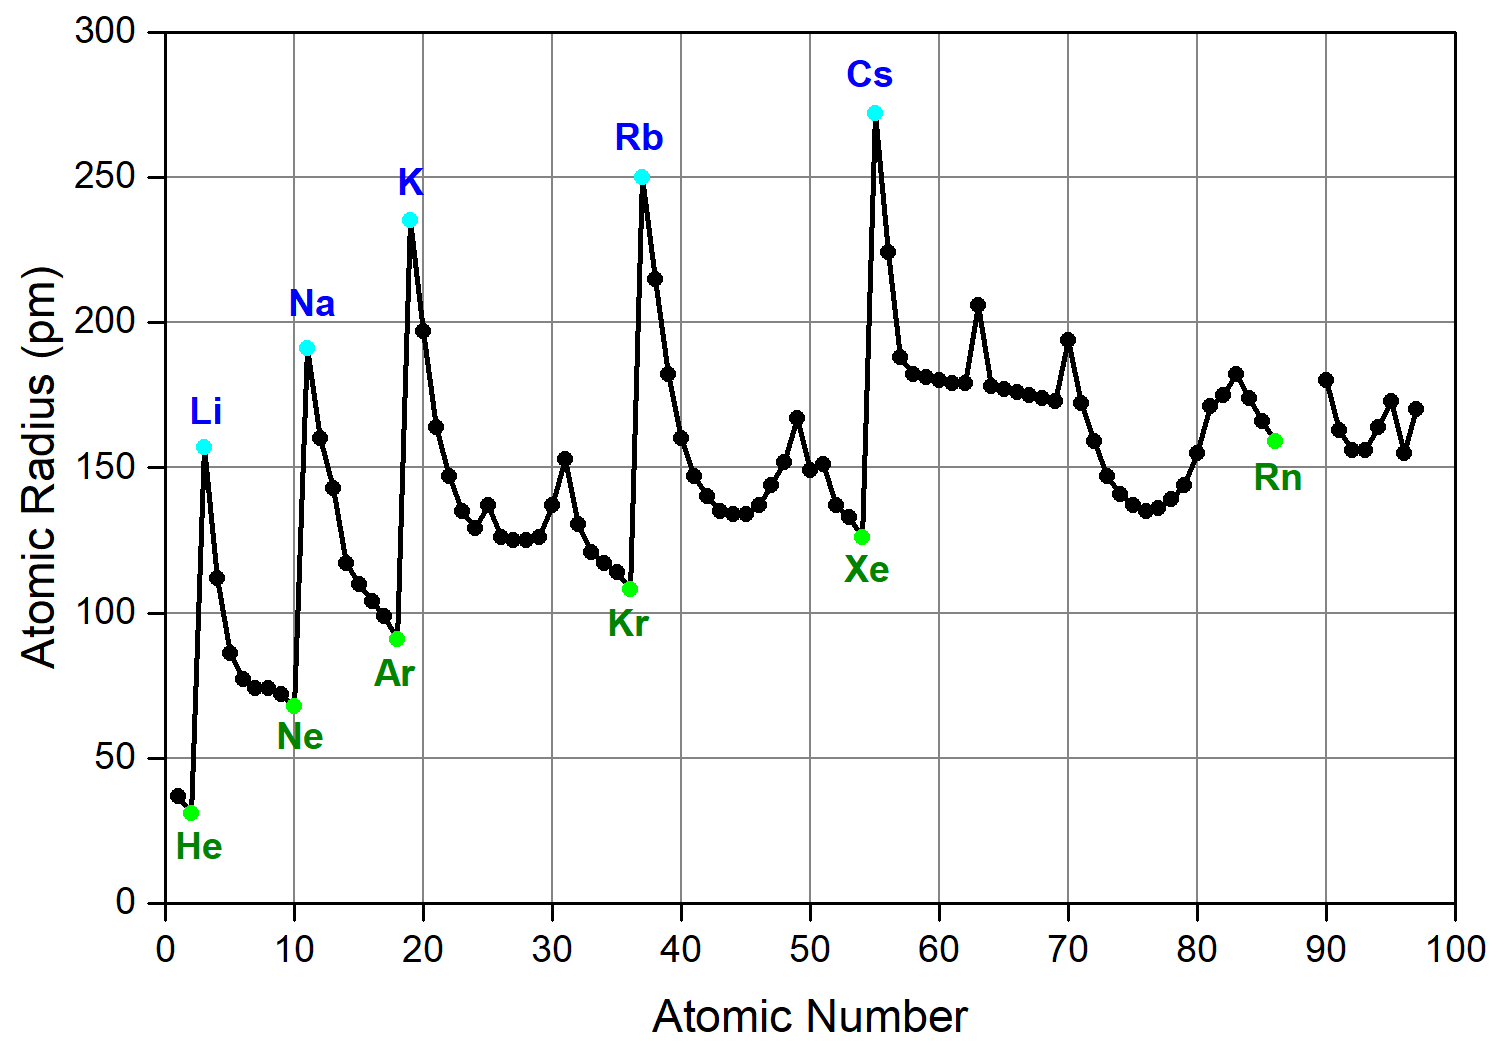
\includegraphics[width=0.45\textwidth]{atom-rad.png}
	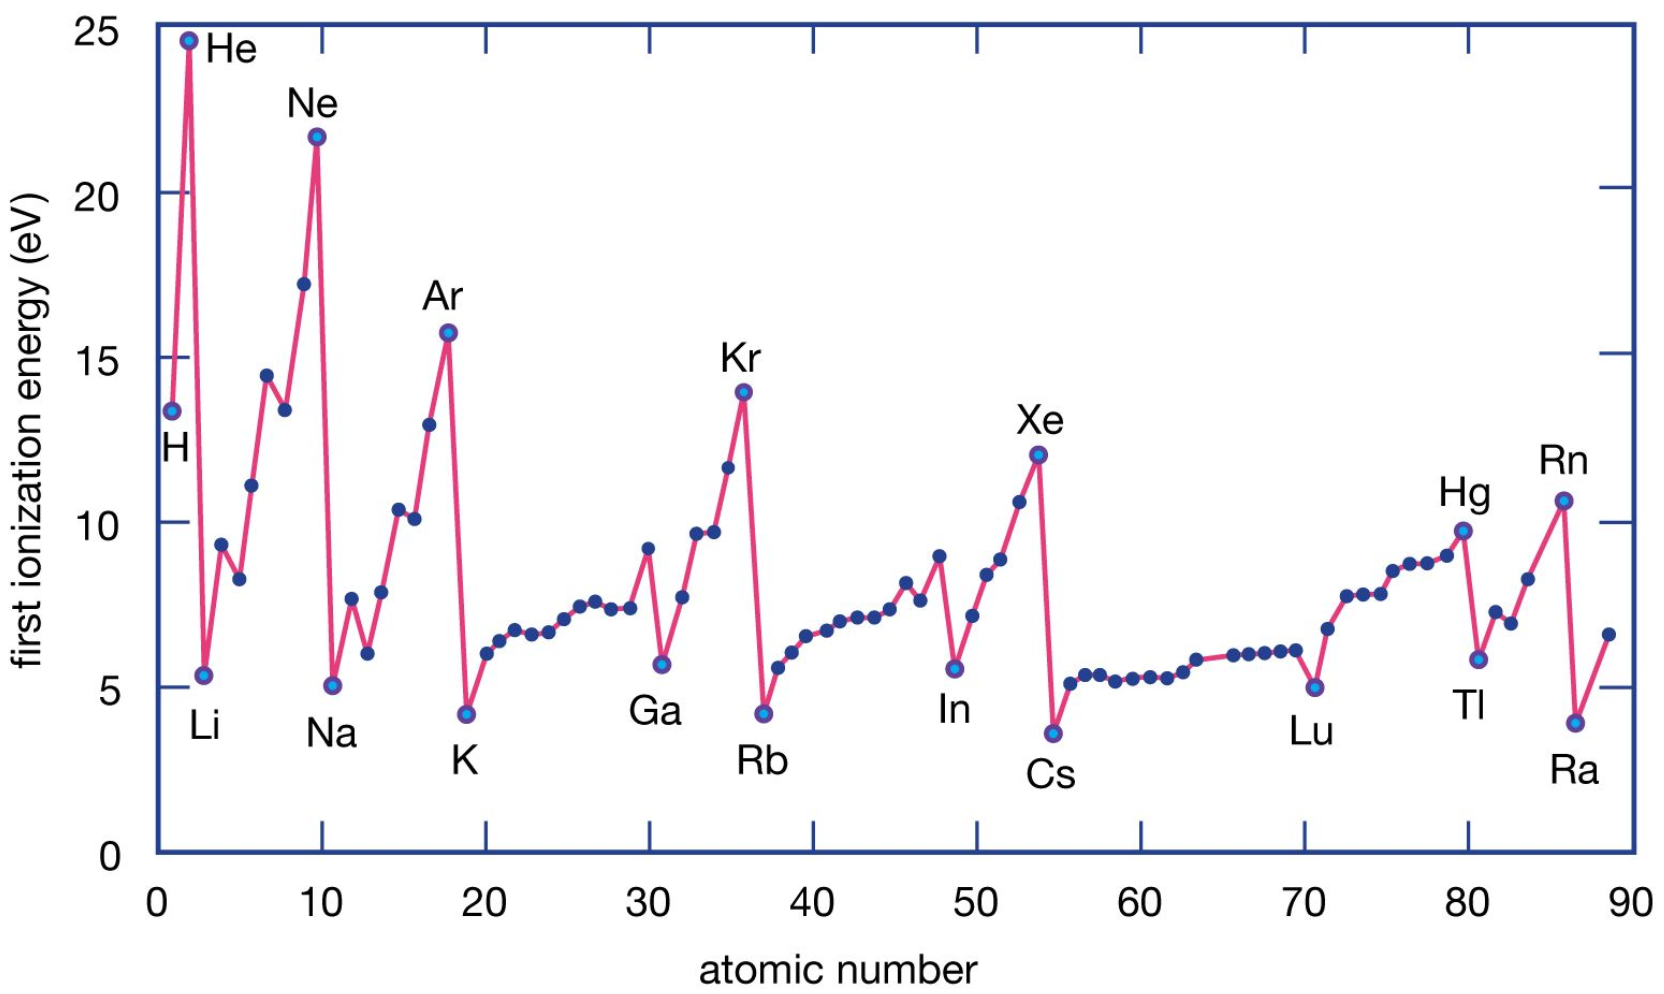
\includegraphics[width=0.52\textwidth]{atomic-ion-en.png}
	\caption{Atomic radius and ionization energy as functions of atomic mass number.}
	\label{atom-prop}
\end{figure}

\subsection{Evidenze sperimentali}

La semplicità del modello atomico a shell non è così immediata da traslare alla fisica nucleare: infatti, mentre gli elettroni nell'atomo sono soggette al campo coulombiano generato dal nucleo atomico, nel nucleo i nucleoni sono soggetti ad un campo che essi stessi generano, rendendo la trattazione analitica estremamente più complicata; inoltre, i nucleoni hanno un raggio relativamente grande rispetto al raggio del nucleo, a differenza degli elettroni che possono essere approssimati come point particles all'interno dell'atomo: ciò rende il concetto di orbite spaziali ben definite difficile da applicare al nucleo, dove il moto dei nucleoni può essere disturbato da urti con altri nucleoni.\\
Nonostante ciò, ci sono varie evidenze sperimentali che suggeriscono l'esistenza di shell nucleari.\\
Innanzitutto, se si plotta la binding energy per nucleone (Fig. \ref{magic-bind-en}), si notano delle consistenti deviazioni dalla formula di Weizsäcker per il liquid drop model in corrispodenza di precisi valori (uguali) di $ N $ e $ Z $, detti magic numbers: 2, 8, 20, 28, 50, 82, 126. Ciò significa che i nuclidi con determinati numeri di neutroni e/o protoni sono più legati, e dunque più stabili, dei nuclidi ad essi adiacenti. Per completezza, si ricordi che il liquid drop model non si applica per $ A < 20 $, poiché tali nuclidi presentano una struttura nucleare più complessa.

\begin{figure}[!t]
	\centering
	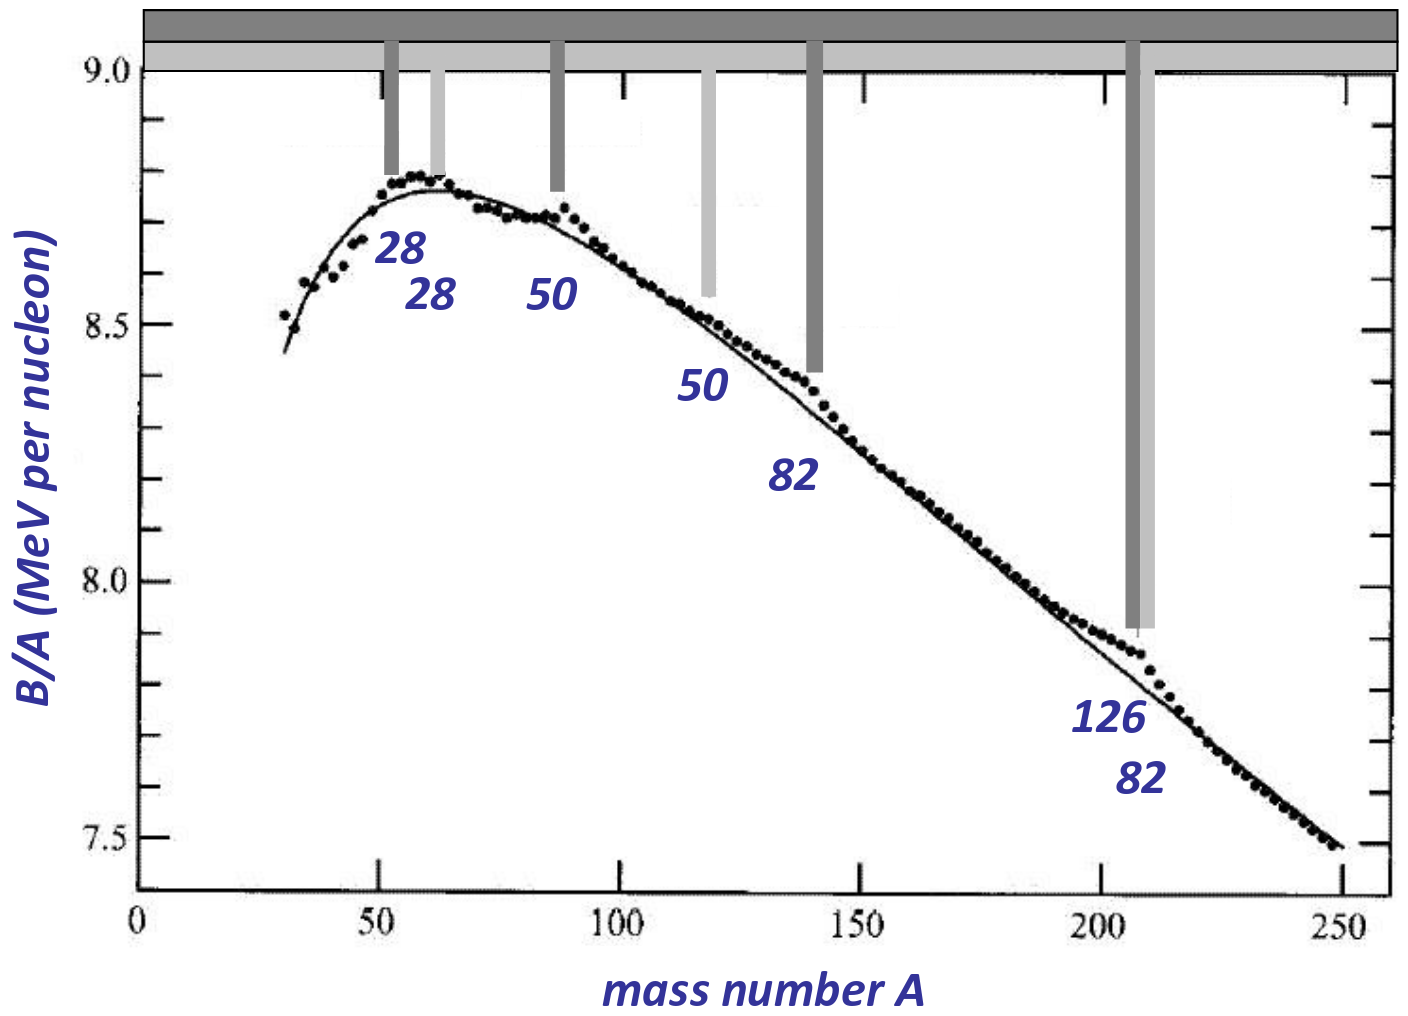
\includegraphics[width=0.60\textwidth]{magic-bind-en.png}
	\caption{Binding energy per nucleon, with $ N $ (dark grey) and $ Z $ (light grey) highlighted.}
	\label{magic-bind-en}
\end{figure}

\begin{figure}[!ht]
	\centering
	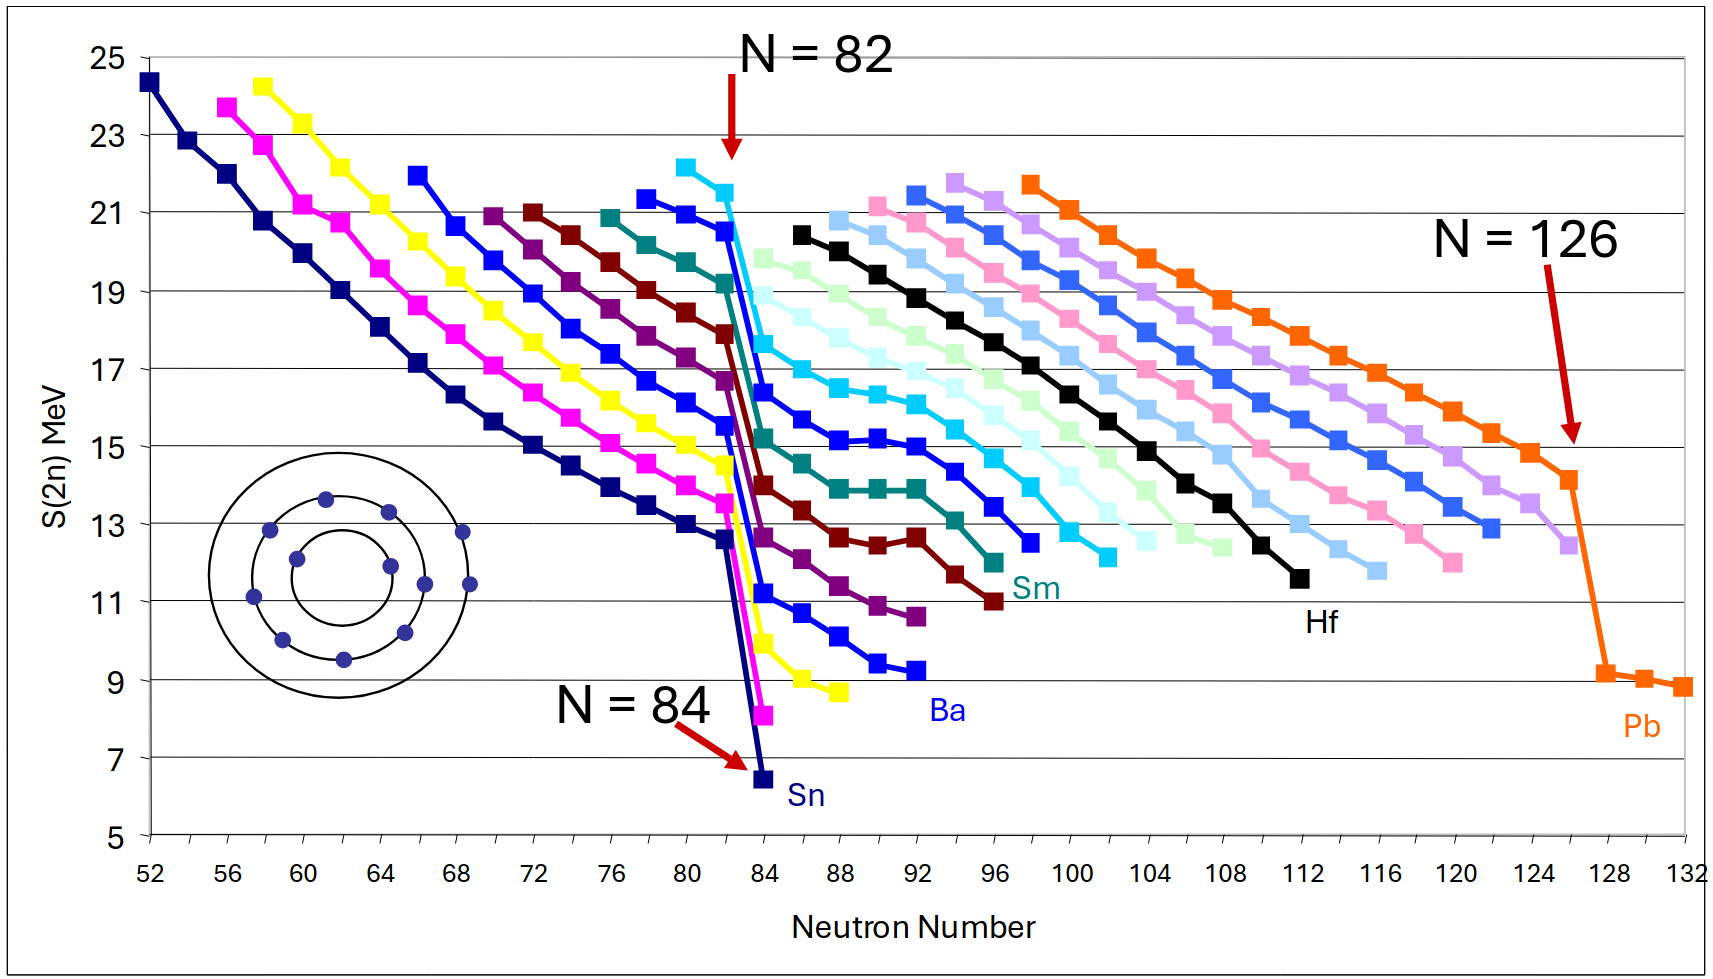
\includegraphics[width=0.60\textwidth]{2-n-b-e.png}
	\caption{2-neutron binding energy as a function of $ N $ for various isotopic chains.}
	\label{2-n-b-e}
\end{figure}

\begin{figure}[!t]
	\centering
	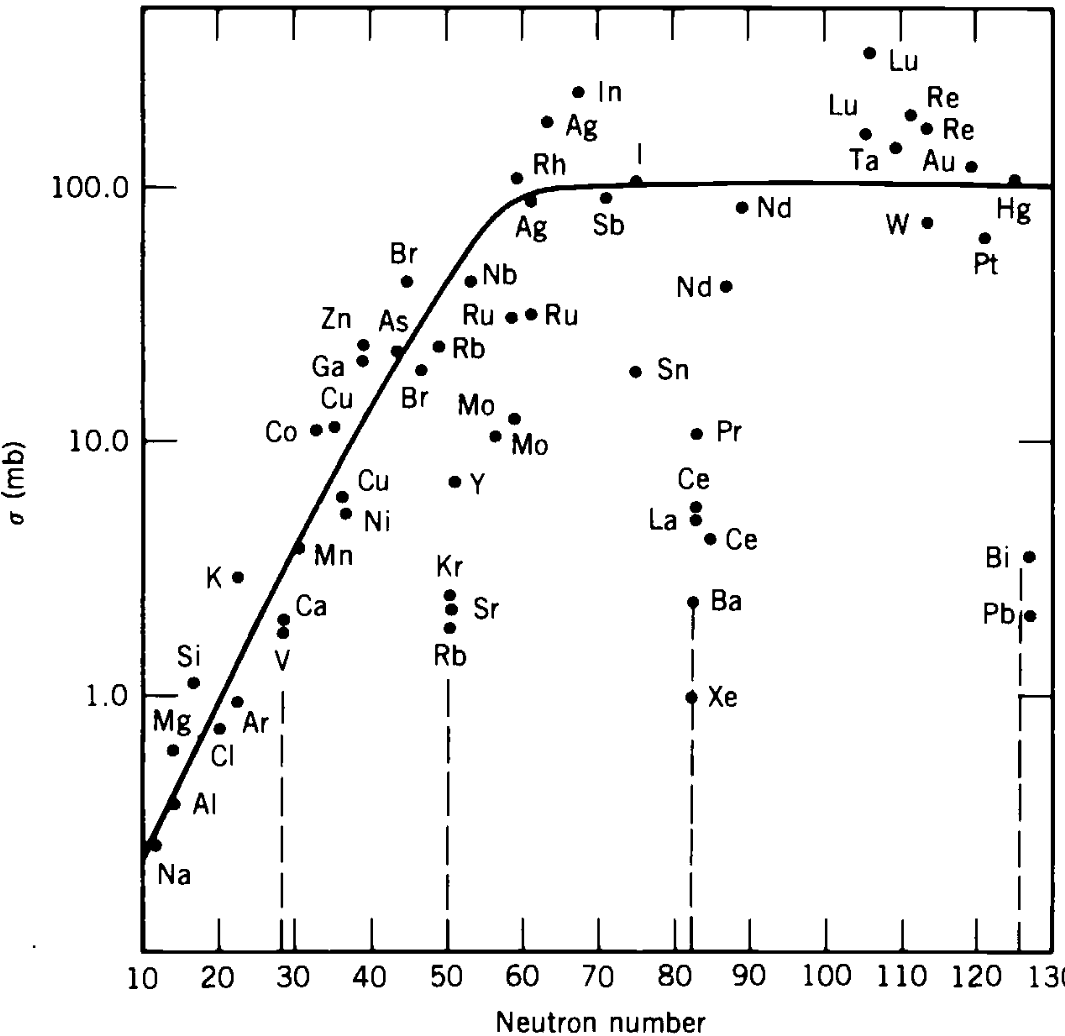
\includegraphics[width=0.60\textwidth]{magic-n-cap.png}
	\caption{$ n $-capture cross-section ad a funzion of.}
	\label{n-cap-cr}
\end{figure}

Gli stessi magic numbers si notano studiando la cosiddetta \textit{2-neutron binding energy}, ovvero la quantità $ S_{2n}(N,Z) \equiv B(N,Z) - B(N-2,Z) $, come si può vedere in Fig. \ref{2-n-b-e}: ciò può essere interpretato come una maggiore stabilità data dal completamento di shell neutroniche.\\
Anche l'abbondanza di isotopi stabili nel sistema solare mostra dei picchi in corrispondenza dei magic numbers, evidenziando la particolare stabilità dei nuclidi con shell closures.\\
Inoltre, la cross-section per la cattura neutronica subisce delle riduzioni di un paio di ordini di grandezza in corrispondenza dei magic numbers (Fig. \ref{n-cap-cr}: ciò è sia conseguenza diretta delle shell closures, sia conseguenza della riduzione del raggio nucleare determinato dalle suddette (dato che $ \sigma \sim \pi R^2 $).
Infine, per nuclei vicini ai magic numbers si osservano degli stati eccitati relativamente long-lived ($ \tau > 10^{-6}\,\text{s} $) detti \textit{isomeri}: i magic numbers determinano delle cosiddette $ \virgolette{islands of isomerism} $.\\
Si deve aggiungere poi che il liquid drop model non consente una descrizione di vari proprietà nucleari come lo spin, la parità, i momenti magnetici etc. Inoltre, esso non predice la densità nucleare e tutti i suoi coefficienti sono puramente empirici.

\subsection{Modello a particelle indipendenti}

Il primo modello a shell in grado di riprodurre i magic numbers e le proprietà dei magic nuclei fu formulato nel 1949 da Mayer e Jensen (entrambi Nobel nel 1963).\\
Il cosiddetto extreme single-particle shell model, detto anche shell model a particelle indipendenti, ha come assunzione di base che i nucleoni possano muoversi nel nucleo per la maggior parte del tempo senza interagire con altri nucleoni: ciò equivale a dire che il libero cammino medio di un nucleone è maggiore delle dimensioni del nucleo. Ovviamente questa è solo una semplificazione, dato che l'interazione tra nucleoni ha effetti importanti.\\
Rispetto allo shell model atomico, quello nucleare deve tener conto di alcune complicazioni: innanzitutto la forma del potenziale non è nota e, qualora lo si volesse assumere centrale, non ha avrebbe un centro definito poiché ciascun nucleone è sorgente del campo; inoltre, i nucleoni occupano il  nucleo in modo continuo, dunque non è ovvio come estendere il concetto di orbitale in questo contesto. Quest'ultima difficoltà è in parte ridotta dal principio d'esclusione di Pauli e dal modello a gas di Fermi\footnote{Un gas di Fermi è un modello ideale di un ensamble di molti fermioni non-interagenti in equilibrio termico, descritto dalla statistica di Fermi-Dirac.}: se il gas di nucleoni è fortemente degenere, ciascun nucleone è in uno stato quantistico e non scattera con un altro nucleone se non con un meccanismo di scambio, il che permette di impostare un'equazione del moto per il singolo nucleone (da qui il nome di modello a particelle indipendenti).\\
Per rendere l'equazione di Schrödinger risolvibile per un singolo nucleone, si applica l'\textit{approssimazione di campo medio}:
\begin{equation*}
	\hat{\mathcal{H}} = \sum_{j = 1}^{A} \frac{\hat{p}_j^2}{2m_j} + \sum_{j \neq k}^{A} \hat{V}_k(r_j) = \sum_{j = 1}^{A} \left[ \frac{\hat{p}_j^2}{2m_j} + \hat{V}(r_j) \right] + \sum_{j = 1}^{A} \underbrace{\left[ \sum_{k \neq j}^{A} \hat{V}_k(r_j) - \hat{V}(r_j) \right]}_{0}
\end{equation*}
dove l'approssimazione consiste nell'ultima semplificazione. Ciò permette di sostituire il termine d'interazione (che è a 2 corpi solo in prima approssimazione) con un potenziale centrale medio, ignorando l'interazione residua. Dato che il potenziale ha simmetria sferica, è possibile separare la funzione d'onda come:
\begin{equation}
	\psi(\ve{r}) = \frac{u_{\ell}}{r} Y_{\ell,m}(\theta,\phi) X_s
	\label{eq:5.3}
\end{equation}
recuperando così gli ususali numeri quantici. Rimane da determinare il potenziale; i tre potenziali usuali sono quello coulombiano, la buca di potenziale e quello armonico: il potenziale coulombiano non è adatto poiché l'interazione nucleare è a breve raggio e poiché non può riprodurre la saturazione delle forze nucleari; la buca di potenziale non è realistica poiché non può riprodurre l'energia cinetica e potenziale dei nucleoni; il potenziale armonico non va a 0 all'infinito, dunque non potrebbe descrivere la fuoriuscita di nucleoni dal nucleo, cosa che avviene se ad esempio viene aggiunto un nucleone ad un nuclide debolmente legato. Il potenziale che meglio rappresenta l'interazione nucleare è il \textit{potenziale di Woods-Saxon}:
\begin{equation}
	V_{\text{WS}}(r) = \frac{-V_0}{1 + e^{(r - R_0) / a}}
	\label{eq:5.4}
\end{equation}
dove $ V_0 \approx 50\mev $ (verso le driplines varia drasticamente), $ R_0 \approx 1.25\fm \cdot A^{1/3} $ è il raggio nucleare medio e $ a \approx 0.524\fm $ è la skin thickness del nucleo (distanza in cui $ V(r) $ passa da $ 0.9 V_0 $ a $ 0.1 V_0 $); esso è plottato in Fig. \ref{woods-saxon}.

\begin{figure}[!b]
	\centering
	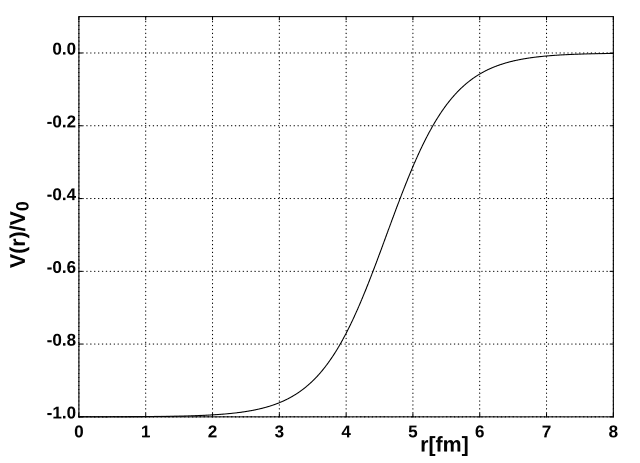
\includegraphics[width=0.70\textwidth]{woods-saxon.png}
	\caption{Woods-Saxon potential.}
	\label{woods-saxon}
\end{figure}

Il potenziale di Woods-Saxon prevede sia gli stati legati, con energia negativa, sia gli stati del continuo, con energia positiva. Gli stati sono giustamente quantizzati con tre numeri quantici: quello principale $ n $, quello angolare orbitale $ \ell $ e quello angolare totale $ j $ (relativo a $ \ve{J} = \ve{L} + \ve{S} $). Gli orbitali nucleari vengono quindi identificati come $ n\ell_j $, dove $ \ell $ è indicato con una lettera: $ s $ per $ \ell = 0 $, $ p $ per $ \ell = 1 $, $ d $ per $ \ell = 2 $, $ f $ per $ \ell = 3 $ e poi in ordine alfabetico.\\
Come si può vedere in Fig. \ref{ws-sp}, il solo potenziale di Woods-Saxon predice correttamente soltanto i primi tre magic numbers. È quindi necessario modificare tale potenziale con un termine di nuovo mutuato dalla fisica atomica: un termine d'interazione spin-orbita. Nel caso atomico, l'interazione spin-orbita avviene poiché il momento magnetico dell'elettrone interagisce col campo magnetico generato dal suo moto attorno al nucleo; nel caso nucleare, essa non deriva dall'interazione elettromagnetica ma dalla natura spin-dependent dell'interazione tra nucleoni.\\
Ricordando l'Eq. \ref{eq:4.20}, si può scrivere il \textit{potenziale d'interazione spin-orbita} come:
\begin{equation}
	V_{\ell,s}(r) \ve{L}\cdot\ve{S} = - \lambda \frac{1}{r} \frac{dV_{\text{WS}}}{dr} \ve{L}\cdot\ve{S}
	\label{eq:5.5}
\end{equation}
dove $ \lambda > 0 $ non ha particolare interesse fisico. Questo termine deriva dalla descrizione relativistica di un singolo nucleone nel nucleo ed è particolarmente importante sulla superficie nucleare (quando $ V_{\text{WS}}(r) $ varia maggiormente).

\begin{figure}[!b]
	\centering
	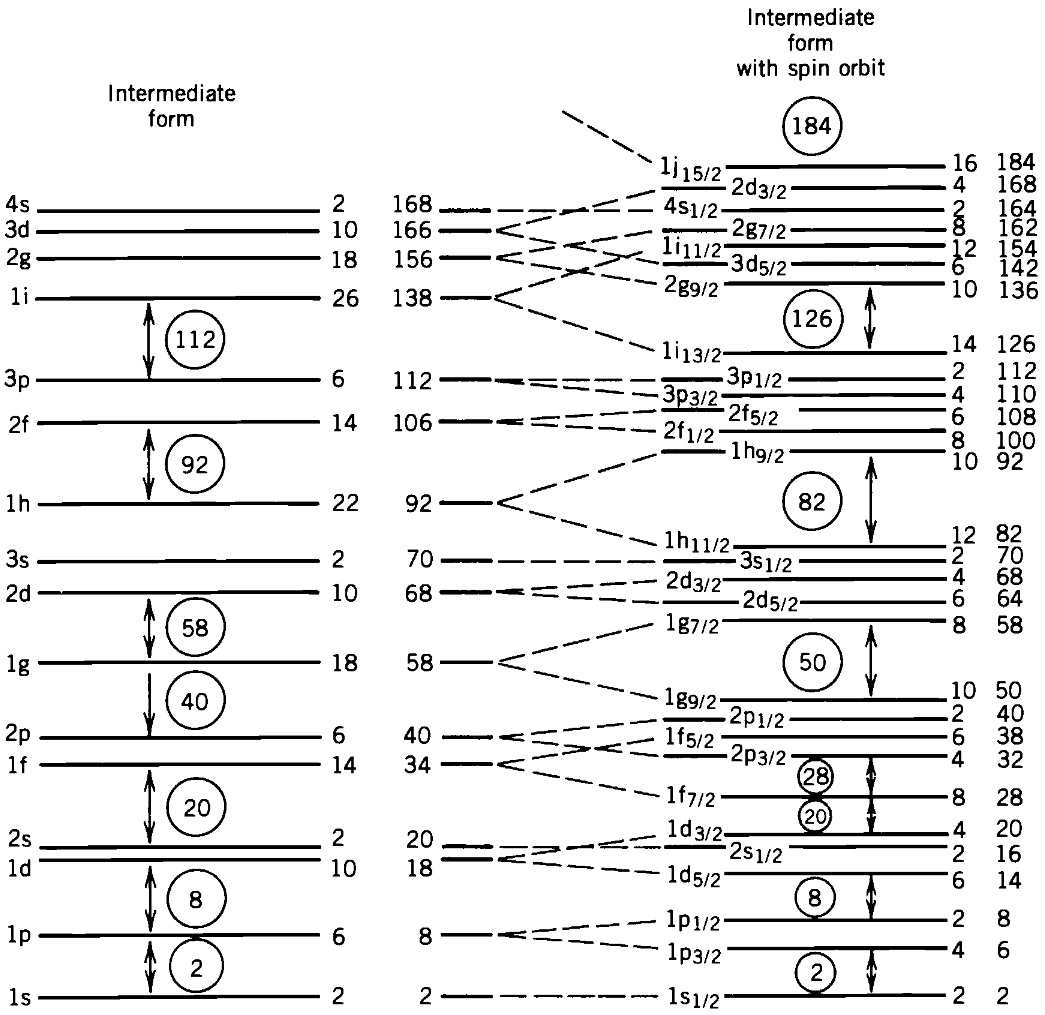
\includegraphics[width=0.60\textwidth]{ws-spectrum.png}
	\caption{Energy levels for the Woods-Saxon potential, without and with spin-orbit interaction.}
	\label{ws-sp}
\end{figure}

Si può vedere come l'aggiunta di questo termine splitti gli orbitali in modo da ottenere i corretti magic numbers. Ricordando che un nucleone ha $ s = \frac{1}{2} $, si vede che i possibili valori per $ j $ sono $ j = \ell + \frac{1}{2} $ e $ j = \ell - \frac{1}{2} $; inoltre, si può lavorare sul termine $ \ve{L}\cdot\ve{S} $:
\begin{equation*}
	\braket{\ve{L}\cdot\ve{S}} = \frac{1}{2} \braket{\ve{J}^2 - \ve{L}^2 - \ve{S}^2} = \frac{\hbar^2}{2} \left[ j (j + 1) - \ell (\ell + 1) - s (s + 1) \right]
\end{equation*}
A questo punto, si deve considerare che i due possibili valori di $ j $ per ogni $ \ell $ portano ad uno split degli orbitali considerati: ad esempio, un orbitale $ 1f $ (con $ \ell = 3 $) viene splittato in $ 1f_{5/2} $ e $ 1f_{7/2} $. Ciascun orbitale così ottenuto ha degenerazione $ 2j + 1 $ determinata da $ m_j $ (con l'interazione spin-orbita, $ m_{\ell} $ ed $ m_s $ non vanno più bene come numeri quantici poiché non sono ben definiti): in questo modo si ottiene comunque la corretta degenerazione totale, poiché $ 2(\ell + \frac{1}{2}) + 1 + 2(\ell - \frac{1}{2}) + 1 = 2(2\ell + 1) $, solo che viene redistribuita asimmetricamente tra due orbitali.\\
Questo splitting porta ad uno splitting anche energetico proporzionale ad $ \ell $, poiché:
\begin{equation}
	\braket{\ve{L}\cdot\ve{S}}_{j = \ell + \frac{1}{2}} - \braket{\ve{L}\cdot\ve{S}}_{j = \ell - \frac{1}{2}} = \frac{\hbar^2}{2} (2\ell + 1)
	\label{eq:5.6}
\end{equation}
Dato che $ V_{\ell,s}(r) < 0 $ (dall'Eq. \ref{eq:5.5}), l'orbitale con $ j $ maggiore ha un'energia più bassa: come si vede in Fig. \ref{ws-sp}, ciò permette di ottenere i corretti magic numbers ed anche di predirne uno nuovo ancora mai osservato: 184.\\
Un'importante conseguenza di questo splitting è che orbitali con diverso $ n $ ed $ \ell $ vengono scambiati di posto nella ladder degli stati: di conseguenza, dato che la parità di un orbitale è $ \pi = (-1)^{\ell} $, orbitali di parità diversa vengono mescolati nella ladder; inoltre, dato che l'interazione forte preserva la parità, orbitali di parità diversa sono ben distinti tra loro e possono essere considerati degli stati puri.

\subsubsection{Nucleoni di valenza}

Il modello a shell, nella sua versione più semplice, ascrive tutte le proprietà di un nuclide dispari (ovvero con $ A $ dispari) al singolo nucleone spaiato nella shell più esterna: se esso si trova nell'orbitale $ n\ell_j $, il ground state del nuclide avrà spin $ j $ e parità $ (-1)^{\ell} $.\\
Nonostante l'estrema semplicità, questo modello predice correttamente il $ J^{\pi} $ di praticamente tutti i nuclidi dispari nel range di masse in cui il modello a shell è valido (ossia $ A < 150 $ e $ 190 < A < 220 $).
Un calcolo più preciso deve ovviamente tener conto almeno di tutti i nucleoni sulla shell di valenza: in tal caso, ciascuno stato eccitato può essere ottenuto mediante varie eccitazioni di nucleoni diversi (sovrapposizione di stati), dette particle-hole eccitations: passando da una shell di energia minore ad una di energie maggiore, il nucleone lascia un buco nella shell minore e questo processo richiede una notevole energia, specialmente se nei pressi degli shell gaps. Anche in questo caso, si ha un buon accordo per nuclidi dispari, specialmente per quelli esprimibili come un doubly magic nuclei + uno o più (pochi) nucleoni (es.: elio, ossigeno, calcio, etc.).\\
In generale (quindi anche per nuclidi pari), ogni orbitale completamente pieno di nucleoni non contribuisce allo spin nucleare, dato che essi si accoppiano in coppie di nucleoni identici con spin opposti (configurazione energeticamente più favorevole).

\subsubsection{Momento magnetico}

Dall'Eq. \ref{eq:4.14}, considerando un $ g_{\ell} $ generico (e non il caso specifico $ g_{\ell} = \frac{1}{2} $), si ha:
\begin{equation}
	g_j = \frac{1}{2} (g_{\ell} + g_s) + \frac{1}{2} \frac{\ell (\ell + 1) - s (s + 1)}{j (j + 1)} (g_{\ell} - g_s)
	\label{eq:5.7}
\end{equation}
I momenti magnetici nucleari possono dunque essere calcolati come:
\begin{equation}
	\braket{\mu} =
	\begin{cases}
		\left[ g_{\ell} (j - \frac{1}{2}) + \frac{1}{2} g_s \right] \mu_N & j = \ell + \frac{1}{2} \\
		\frac{j}{j + 1} \left[ g_{\ell} (j + \frac{3}{2}) - \frac{1}{2} g_s \right] \mu_N & j = \ell - \frac{1}{2}
	\end{cases}
	\label{eq:5.8}
\end{equation}
Queste sono le cosiddette \textit{linee di Schmidt} e, se moltiplicate per un fattore di scala di circa $ 0.60 $, riproducono il trend seguito dai dati sperimentali, come si può vedere in Fig. \ref{schmidt}.

\begin{figure}[!t]
	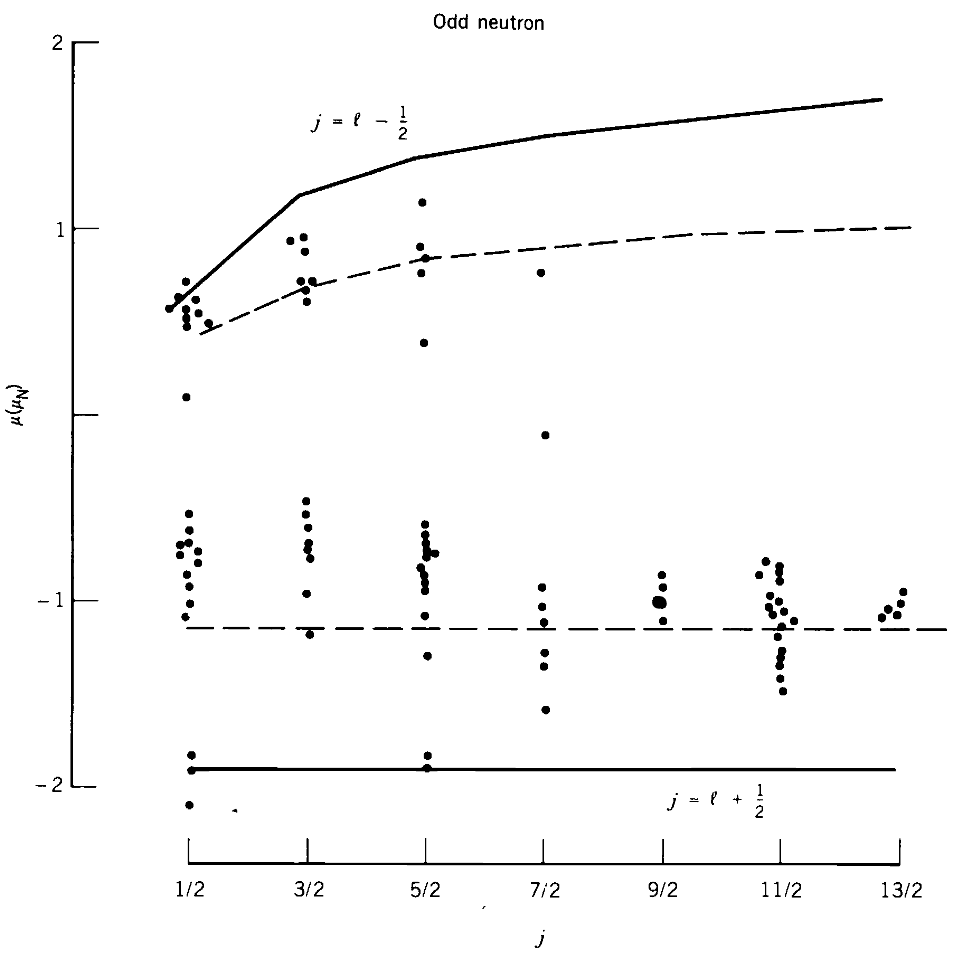
\includegraphics[width=0.60\textwidth]{schmidt-1.png}
	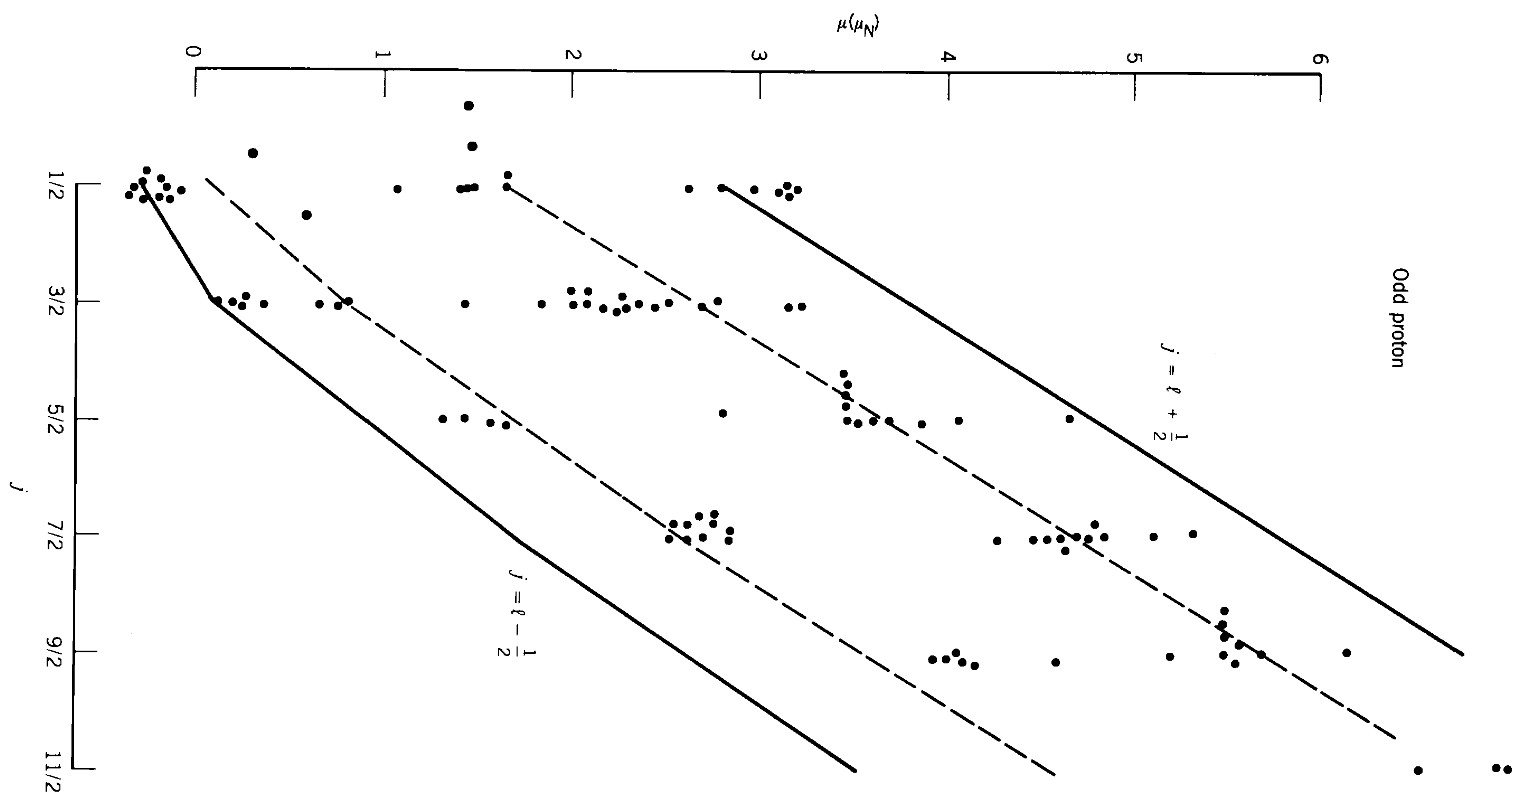
\includegraphics[angle=90,width=0.35\textwidth]{schmidt-2.png}
	\caption{Schmidt lines.}
	\label{schmidt}
\end{figure}

Lo scatter dei dati rispetto alle linee di Schmidt indica che il calcolo del momento magnetico considerando i nucleoni come indipendenti è una semplificazione eccessiva; per un calcolo più preciso, si dovrebbero considerare degli effetti non-banali come l'influenza reciproca dei nucleoni, il fatto che lo spin pairing non sia perfetto, le nubi mesoniche che circondano i nucleoni (che contengono pioni $ \pi^{\pm} $ carichi) e la non sfericità dei nuclei.

\subsubsection{Interazione residua}

Per dare una descrizione unificata di tutti i nuclidi, è necessario aggiungere allo shell model la descrizione dell'interazione residua che viene ignorata nel modello. Ad esempio, per nuclei leggeri è necessario considerare interazioni nucleari a tre o più corpi, problemi difficoltosi da trattare in QCD.\\
Ad oggi, un modo computazionalmente efficiente di calcolare l'interazione residua è dividere il nuclide in un core composto dal più vicino doubly-magic nuclei ($ \ch{^4He} $, $ \ch{^{16}O} $, $ \ch{^{40}Ca} $, $ \ch{^{132}Sn} $ e $ \ch{^{208}Pb} $), il quale rimane freezato e non viene considerato nelle interazioni, e le rimanenti shell d'interazione. Dato che il numero di modi di distribuire $ k $ nucleoni su $ n $ orbitali è pari a $ \binom{n}{k} $, che aumenta fattorialmente all'aumentare dei nucleoni, per snellire ulteriormente il calcolo dal punto di vista computazionale si può ulterioremente restringere l'insieme dei nucleoni sui quali calcolare l'interazione residua alla sola shell di valenza.\\
Anche in questo caso ci sono però delle limitazioni, prime su tutti il considerare solo i nucleoni di valenza e l'ignorare completamente le eccitazioni del core.\\
I principali filoni di ricerca a livello computazionale riguardano da un lato la risoluzione numerica della many-body hamiltonian, dall'altro lo studio delle interazioni nucleari.

\section{Collective models}

Il modello a shell descrive molto bene i nuclidi nell'intorno dei magic numbers, per i quali vale l'approssimazione di campo medio. Quando però si considerano nuclei lontani da tali regioni, i dati sperimentali si discostano dalle previsioni del modello a shell: si osservano fenomeni non riconducibili ad eccitazioni individuali di nucleoni che suggeriscono un comportamento collettivo del sistema.

\subsection{Evidenze sperimentali}

La principale limitazione del modello a shell è l'assunzione che il nucleo sia sferico: ciò è approssimativamente vero solo per nuclei vicini ai doubly-magic nuclei, i quali hanno una doppia shell closure, ma in generale non è vero. La deformazione dei nuclidi lontani dai magic numbers è suggerita da varie evidenze sperimentali, come un grande momento di quadrupolo elettrico (discostamento dalla simmetria di carica), una bassa excitation energy ($ < 1\mev $) per il primo stato eccitato nei nuclei pari-pari (quasi sempre il $ 2^+ $) ed un rapporto costante $ E(4^+) / E(2^+) $ sempre per nuclei pari-pari.

\subsubsection{Momento di quadrupolo elettrico}

Ricordando la definizione in Eq. \ref{eq:4.16}, i momenti di multipolo elettrico forniscono una descrizione della distribuzione di carica (dunque dei protoni) nel nucleo.\\
Dato che i momenti dispari devono essere nulli per la conservazione della parità e che $ K_0 = Ze $ non è altro che la carica totale, il primo parametro utile a verificare la deviazione della distribuzione di carica da una forma sferica è il momento di quadrupolo elettrico $ K_2 \equiv Q $, definito in Eq. \ref{eq:4.17}: assumendo che le distribuzioni di protoni e neutroni non siano troppo diverse tra loro (vero nella valle di stabilità), si può prendere il momento di quadrupolo elettrico come un indicatore della deformazione del nucleo stesso.\\
Considerando un nucleo a forma di ellissoide con sezione circolare di raggio $ a $ sul piano $ xy $ e semiasse $ b $ sull'asse $ z $, si può definire un parametro di deformazione $ \beta $ in funzione del raggio medio $ \braket{R} = (ab^2)^{1/3} $ e della differenza dei semiassi $ \Delta R = b - a $:
\begin{equation}
	\beta = \frac{4}{3} \sqrt{\frac{\pi}{5}} \frac{\Delta R}{\braket{R}}
	\label{eq:5.9}
\end{equation}
In base al segno di $ \beta $, si può stabilire se il nucleo è sferico ($ \beta = 0 $), prolato (allungato lungo $ z $, $ \beta > 0 $) o oblato (schiacciato su $ xy $, $ \beta < 0 $). Il momento di quadrupolo elettrico è legato a $ \beta $ da:
\begin{equation}
	Q_0 = \frac{3}{\sqrt{5\pi}} Z \braket{R}^2 \beta (1 + 0.16 \beta)
	\label{eq:5.10}
\end{equation}
Si noti che $ Q_0 $ è il momento di quadrupolo intrinseco, ovvero misurato nel RF solidale al nuclide; il momento misurato in laboratorio $ Q $ è legato a $ Q_0 $ da una relazione che varia per i vari stati eccitati: per lo stato $ 2^+ $, si ha $ Q = - \frac{2}{7} Q_0 $.
Come si può vedere in Fig. \ref{quad-mom}, i nuclei vicini ai magic numbers sono praticamente sferici, mentre quelli lontani da essi sono deformati: in particolare, i nuclei delle terre rare sono stabilmente deformati. Inoltre, si nota una prevalenza di nuclei prolati rispetto a quelli oblati.

\begin{figure}[!t]
	\centering
	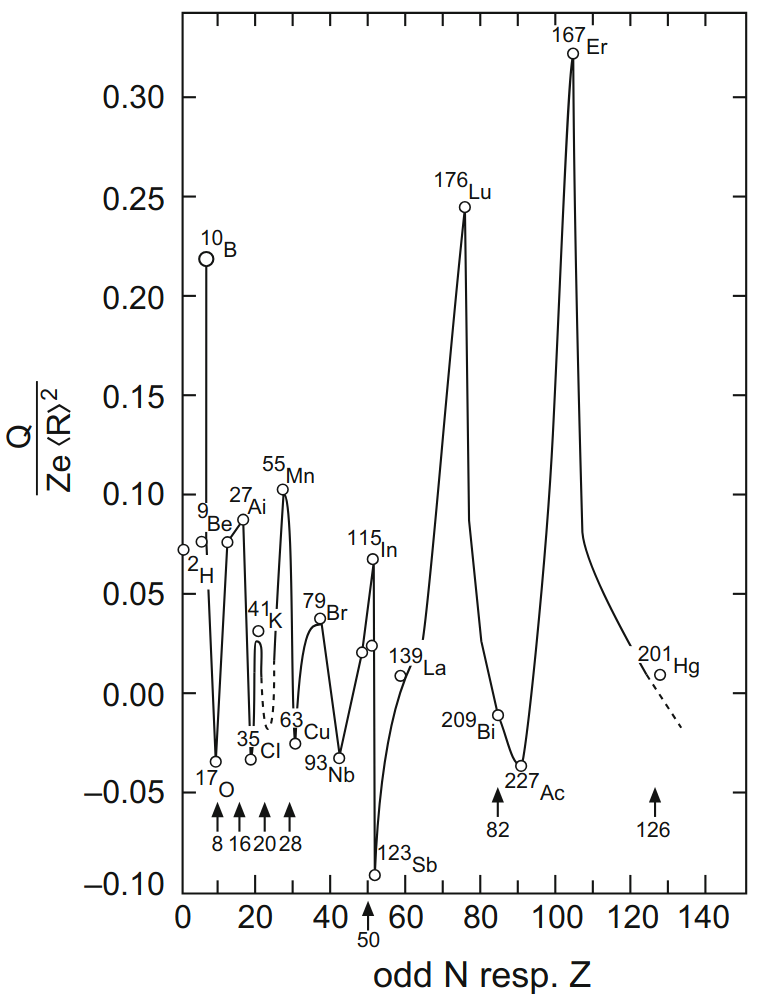
\includegraphics[width=0.60\textwidth]{quad-mom.png}
	\caption{Nuclear electric quadrupole moments for nuclei with odd nucleons.}
	\label{quad-mom}
\end{figure}

\subsubsection{Energia dello stato \texorpdfstring{$ 2^+ $}{TEXT}}

Mentre le eccitazioni dei nuclei dispari sono spiegate bene dal modello a shell, per i nuclei pari-pari il modello non funziona, in quanto in prima approssimazione tutti gli spin dei nucleoni si dovrebbero accoppiare a 0: con tale modello, dunque, è difficile spiegare i loro stati eccitati.\\
Per i nuclei pari-pari, il ground state è lo stato $ 0^+ $ ed il primo stato eccitato è lo stato $ 2^+ $: per spiegare questo stato col modello a shell, sarebbe necessario rompere una coppia di nucleoni appaiati ed eccitarli su livelli distinti, impiegando una notevole quantità di energia ($ \approx 2\mev $). Studiando le energie degli stati $ 2^+ $, però, si vede (Fig. \ref{2-p}) che tale soglia è raggiunta solo nei pressi delle shell closures, mentre normalmente si hanno energie al di sotto di $ 1.2\mev $ con un trend decrescente, fino ad arrivare a $ 100\kev $ per nuclidi pesanti; si nota inoltre che per $ 150 < A < 190 $ e $ A > 230 $ l'energia $ E(2^+) $ è praticamente costante.\\
Da queste osservazioni si conclude che, per realizzare il primo stato $ 2^+ $, questi nuclei assumano una configurazione intrinsecamente più conveniente a livello energetico rispetto alla rottura di una coppia nucleonica.

\begin{figure}[!t]
	\centering
	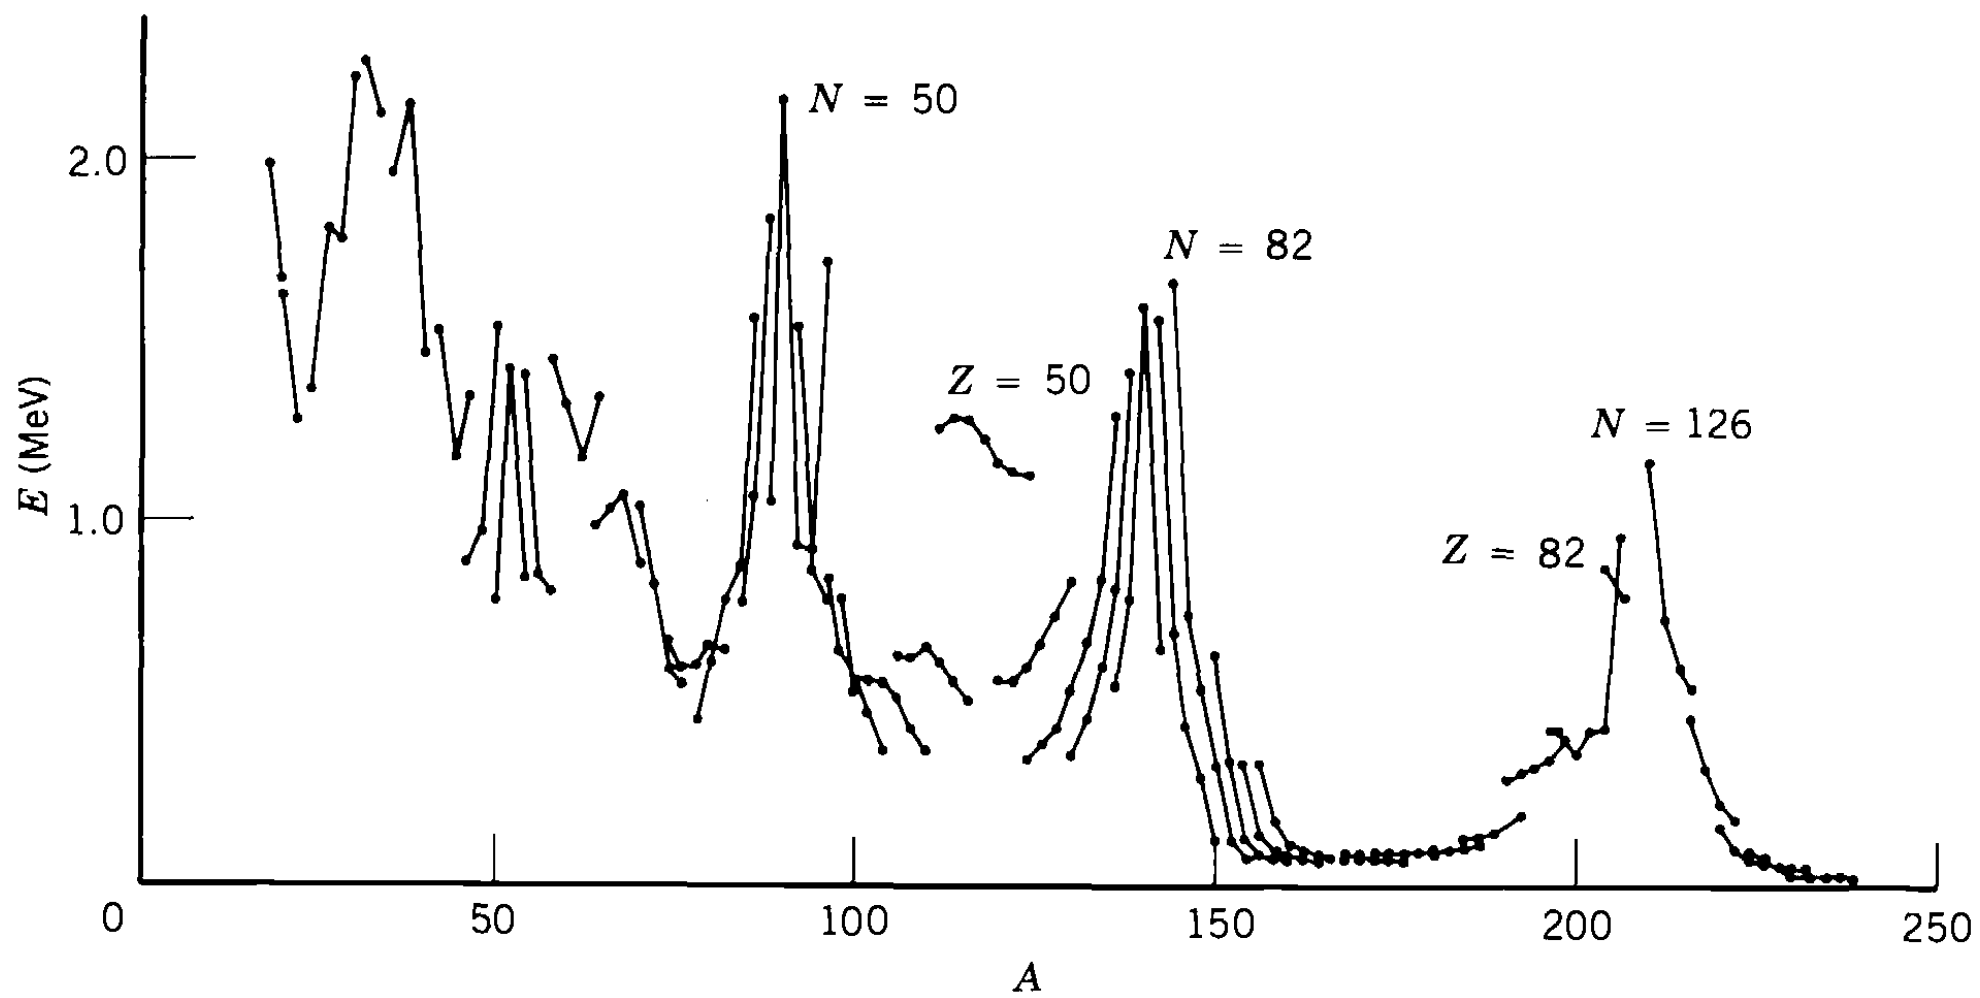
\includegraphics[width=0.70\textwidth]{2-p.png}
	\caption{Energies of lowest $ 2^+ $ states of even-even nuclei, with isotopic chains connected.}
	\label{2-p}
\end{figure}

\subsubsection{Andamento anomalo di \texorpdfstring{$ E(4^+) / E(2^+) $}{TEXT} e \texorpdfstring{$ Q(2^+) $}{TEXT}}

\begin{figure}[!b]
	\centering
	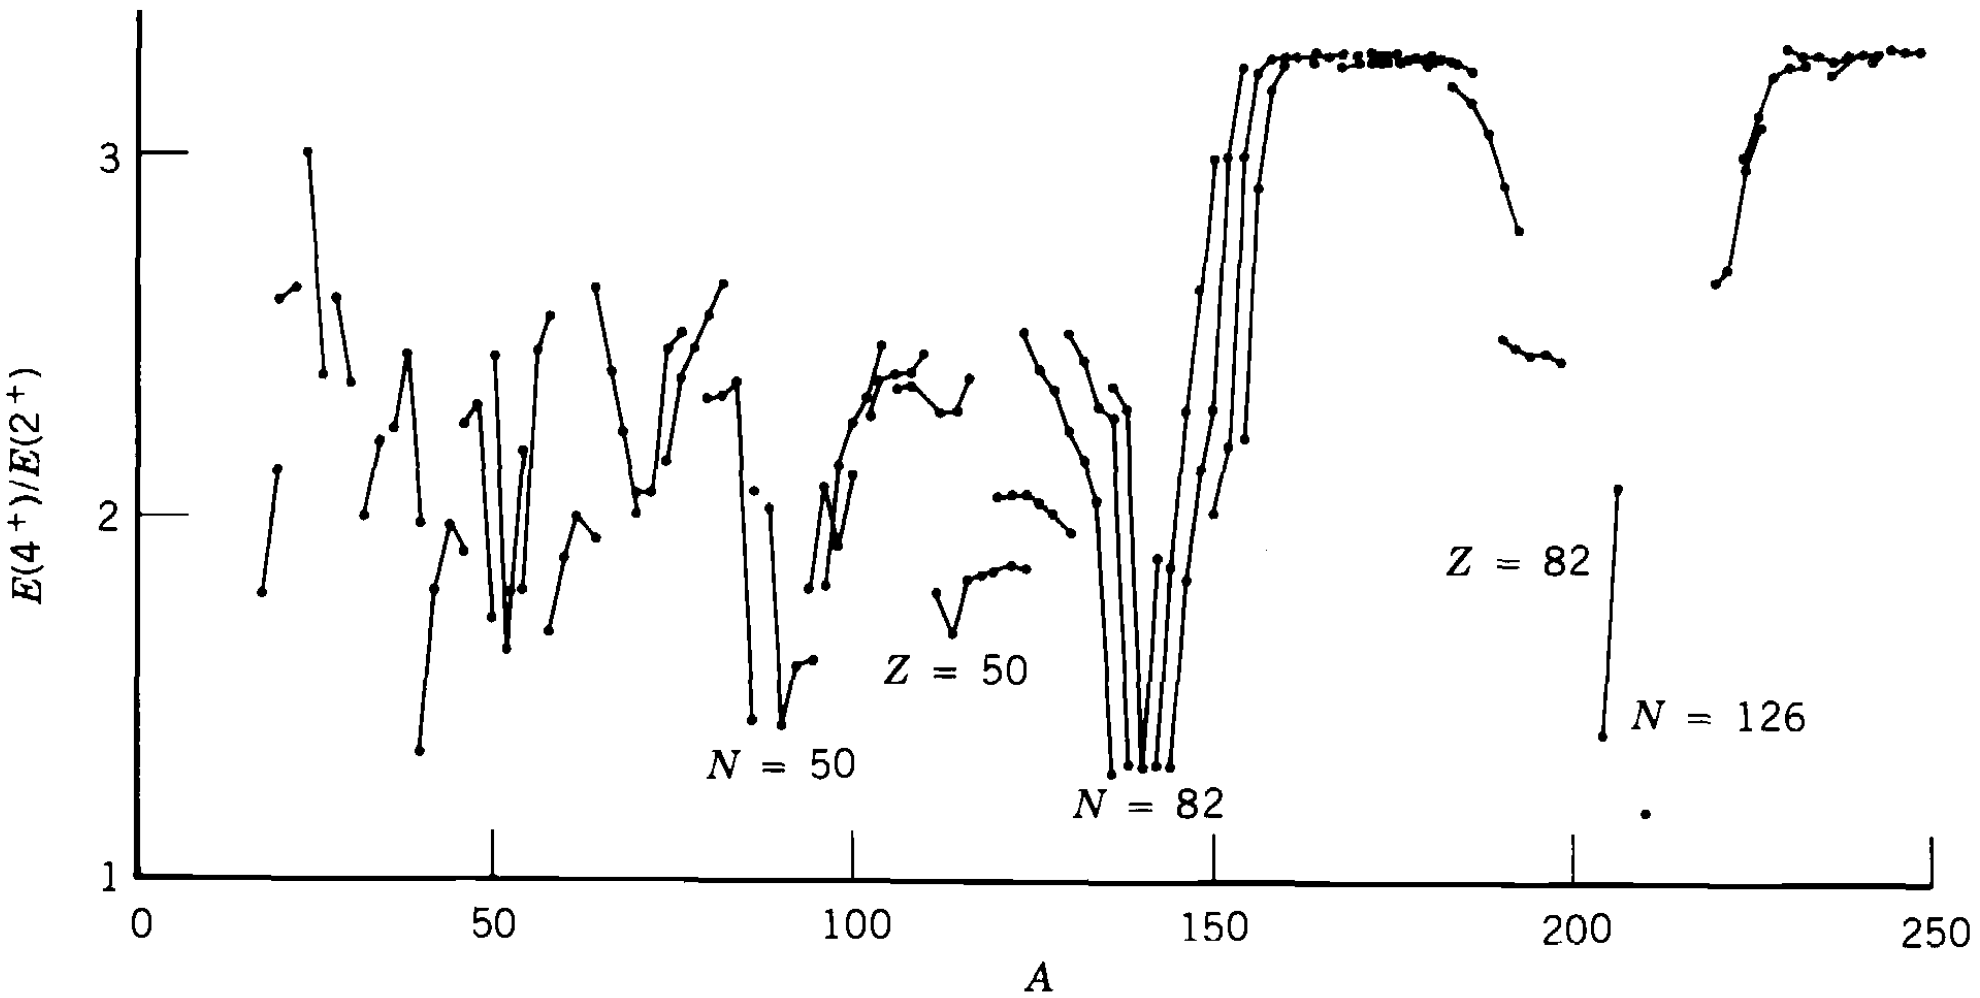
\includegraphics[width = 0.54 \textwidth]{4-p-2-p.png}
	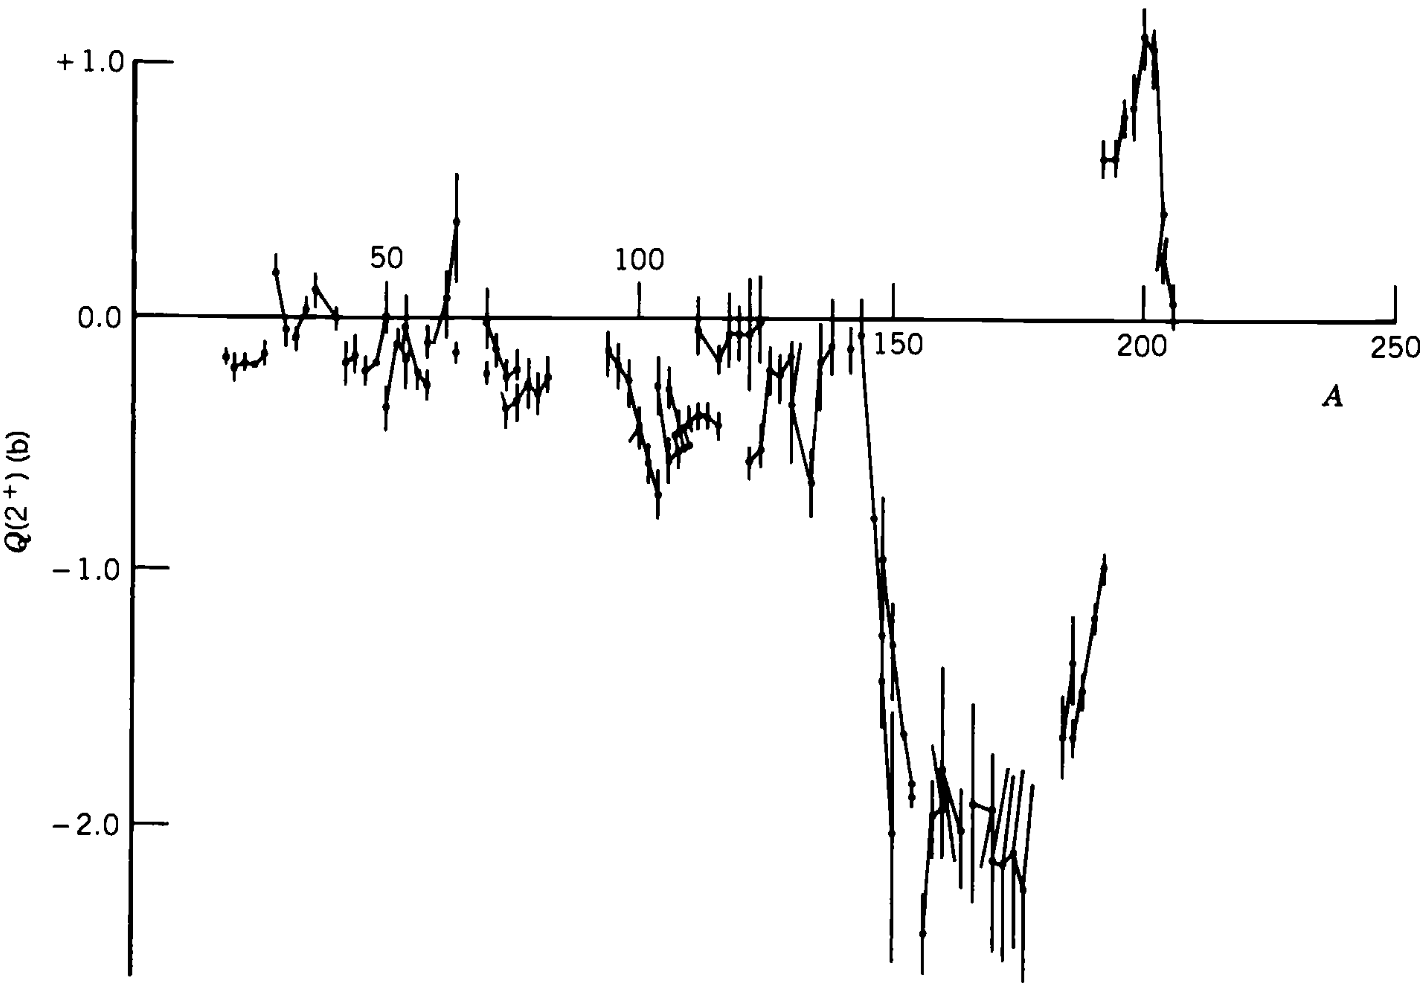
\includegraphics[width = 0.45 \textwidth]{q-2.png}
	\caption{$ E(4^+) / E(2^+) $ ratio and $ Q(2^+) $ for even-even nuclei.}
	\label{4-p-2-p}
\end{figure}

Studiando il rapporto delle energie per i primi stati eccitati $ 2^+ $ e $ 4^+ $ dei nuclei pari-pari (Fig. \ref{4-p-2-p}) si nota che per $ A < 150 $ c'è uno scatter attorno al valore 2, mentre per $ 150 < A < 190 $ e $ A > 230 $ il rapporto ha un valore costante pari a 3.3, indipendentemente dal nuclide considerato.\\
Un trend simile si evidenzia nello studio del momento di quadrupolo magnetico per lo stato $ 2^+ $ (Fig. \ref{4-p-2-p}): per $ A < 150 $ questo momento è circa nullo (a parte deformazioni lontane dalle shell closures), mentre si hanno importanti deviazioni per $ A > 150 $.

\subsubsection{Moti nucleari collettivi}

Tutte queste evidenze sperimentali suggeriscono due tipi diversi di moti nucleari collettivi: le vibrazioni collettive e le rotazioni collettive (vedere Fig. \ref{coll}). Questi moti collettivi avvengono assieme alle eccitazioni single particle del modello a shell e danno una spiegazione a stati che lo shell model non prevede.\\
Per nuclei con $ A < 150 $ si hanno principalmente delle vibrazioni attorno ad una forma sferica: la forma media nel tempo è comunque quella sferica, ma le eccitazioni causano delle vibrazioni collettive del sistema; la sequenza degli stati eccitati generati dalle vibrazioni collettive è energeticamente equispaziata e ha forma $ E_n = n \hbar \omega $.\\
Nuclei con $ A > 150 $ invece sono permanente deformati e hanno un moto rotatorio collettivo; le eccitazioni hanno energia $ E_{I} = \frac{\hbar^2}{2\mathfrak{I}} I (I + 1) $, con $ \mathfrak{I} $ il momento d'inerzia del nucleo e $ I $ il quantum number associato al momento angolare totale (sia neutroni che protoni), dunque sono progressivamente sempre più energeticamente separate.

\begin{figure}[!t]
	\centering
	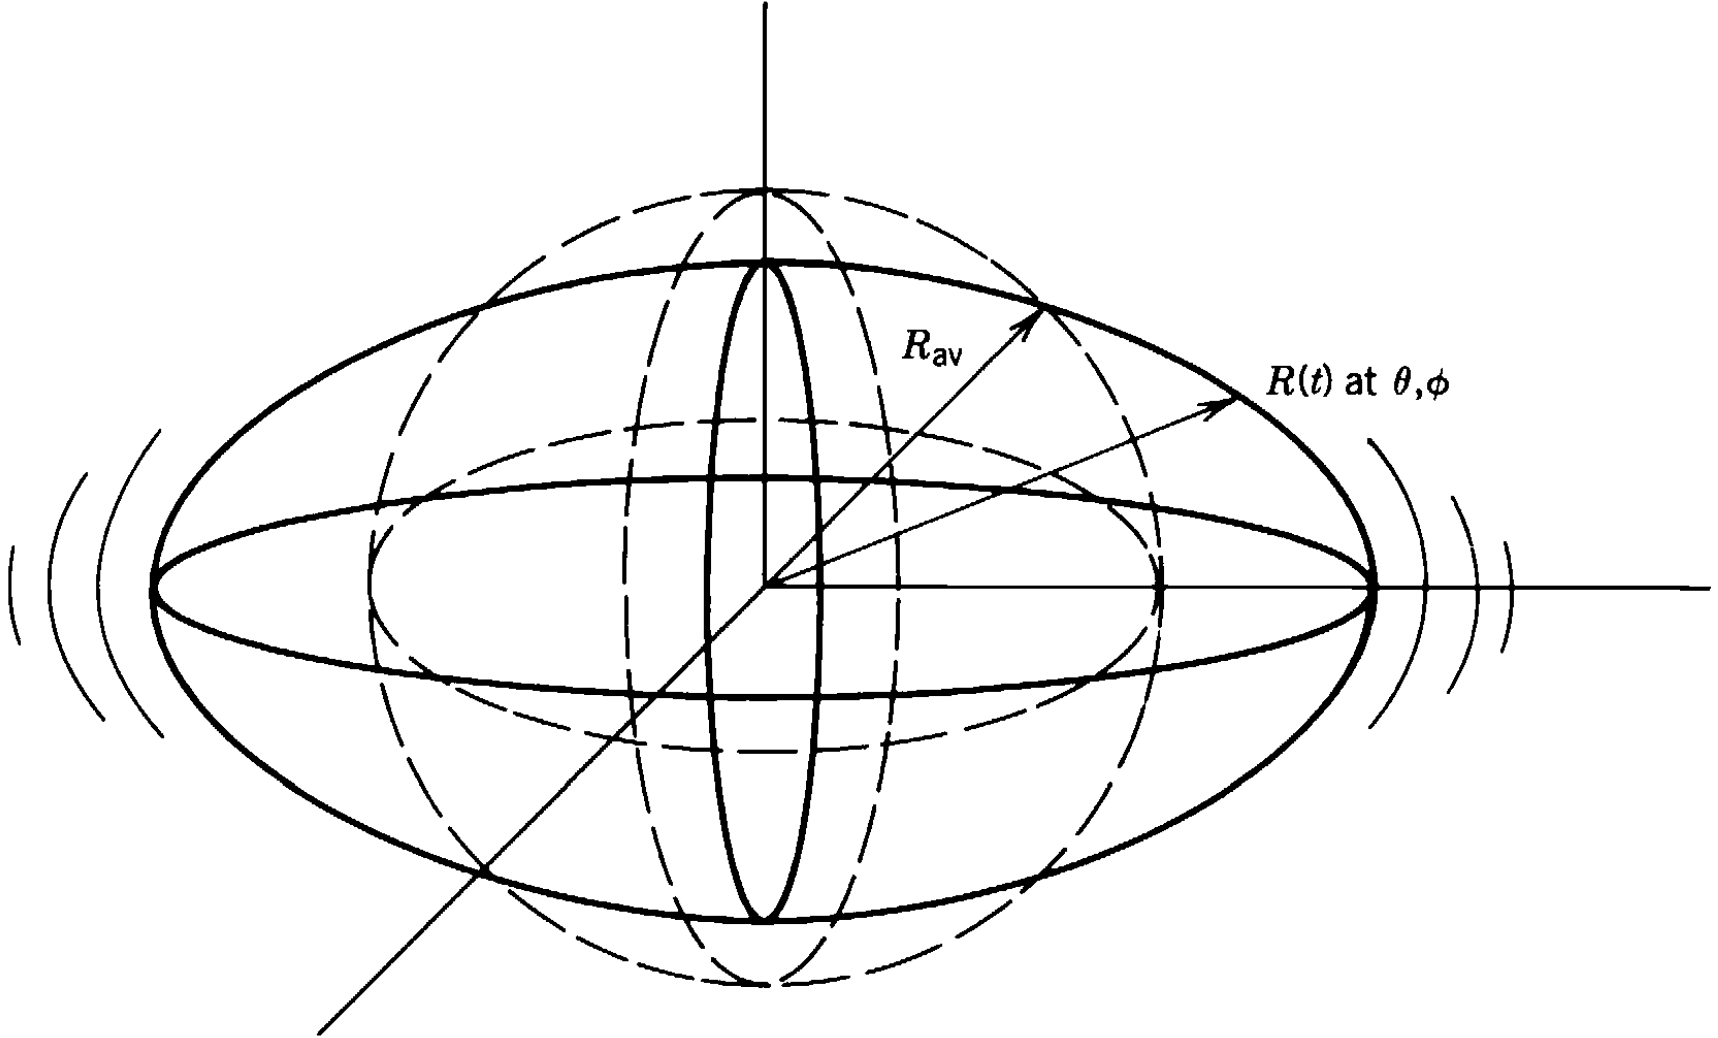
\includegraphics[width = 0.40 \textwidth]{coll-vib.png}
	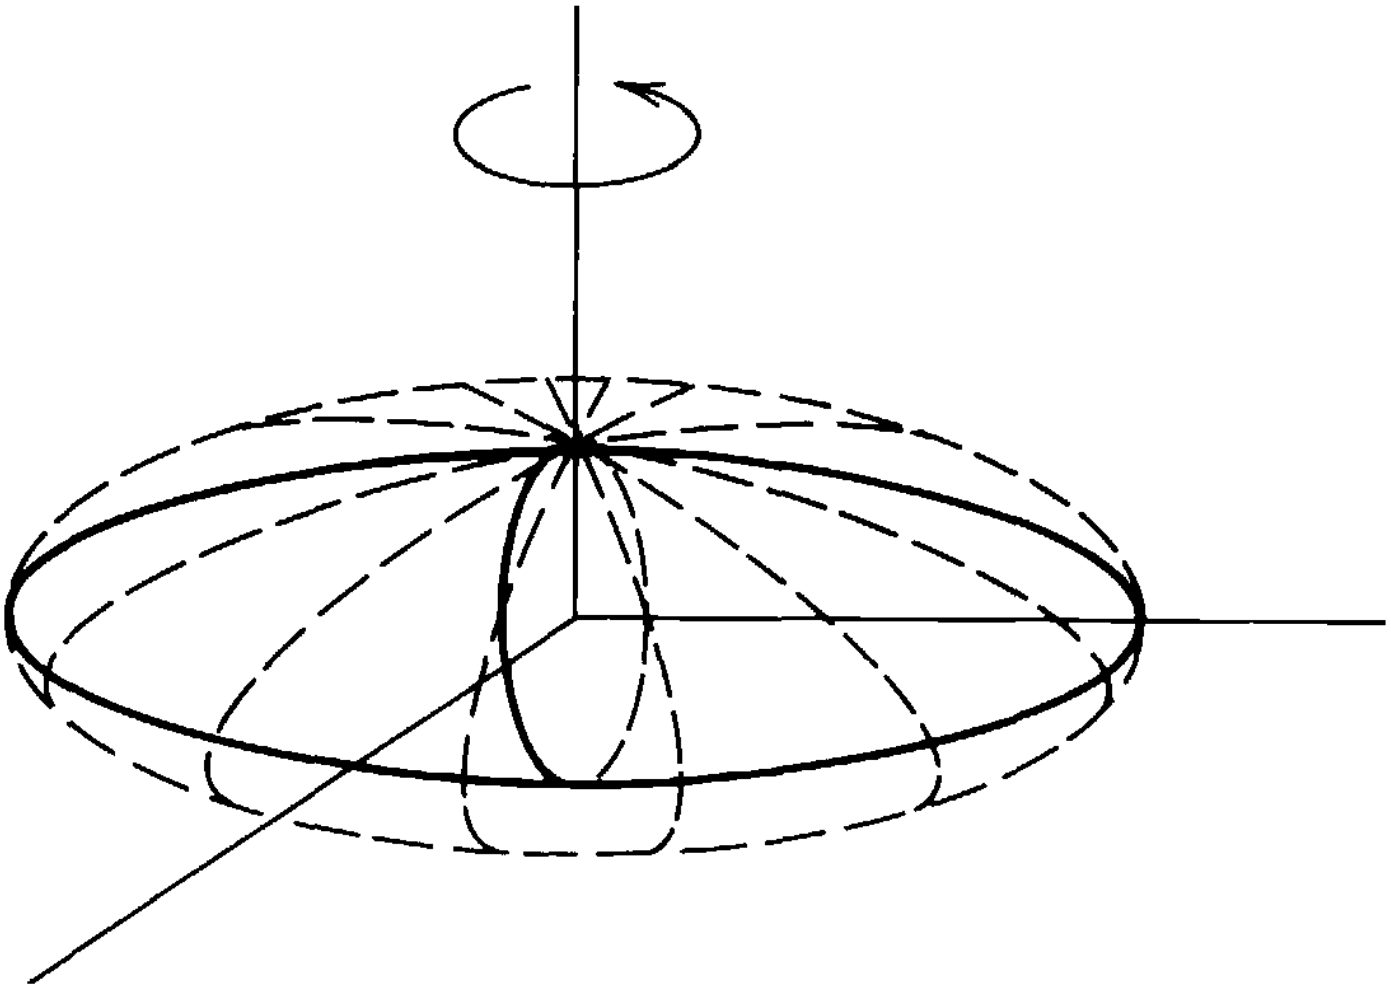
\includegraphics[width = 0.40 \textwidth]{coll-rot.png}
	\caption{Collective vibrations and rotations.}
	\label{coll}
\end{figure}

\subsection{Collective vibrations}

Sebbene la forma media del nucleo sia sferica, per $ A < 150 $, dato che esso può vibrare, la forma istantanea sarà deformata e descrivibile tramite le armoniche sferiche:
\begin{equation}
	R(\theta,\phi,t) = \braket{R} + \sum_{\lambda \ge 1} \sum_{\mu = -\lambda}^{\lambda} \alpha_{\lambda,\mu}(t) Y_{\lambda,\mu}(\theta,\phi)
	\label{eq:5.11}
\end{equation}
I coefficienti $ \alpha_{\lambda,\mu} $ non sono completamente arbitrari, ma per la simmetria di riflessione devono soddisfare $ \alpha_{\lambda,\mu} = \alpha_{\lambda,-\mu} $ (ulteriori condizioni sono imposte dall'eventuale incomprimibilità).\\
I vari termini $ \lambda $ della sommatoria trasportano un quanto di energia vibrazionale, quindi, in analogia all'elettromagnetismo, vengono detti \textit{fononi}. Ad esempio, un fonone dipolare è un quanto di energia vibrazionale con $ \lambda = 1 $ (ovvero trasporta un unità di momento angolare), un fonone quadripolare ha $ \lambda = 2 $, etc. In Fig. \ref{phon} si può vedere che un fonone dipolare causa uno spostamento del centro di massa del nucleo, dunque non può essere il risultato di forze nucleari.

\begin{figure}[!t]
	\centering
	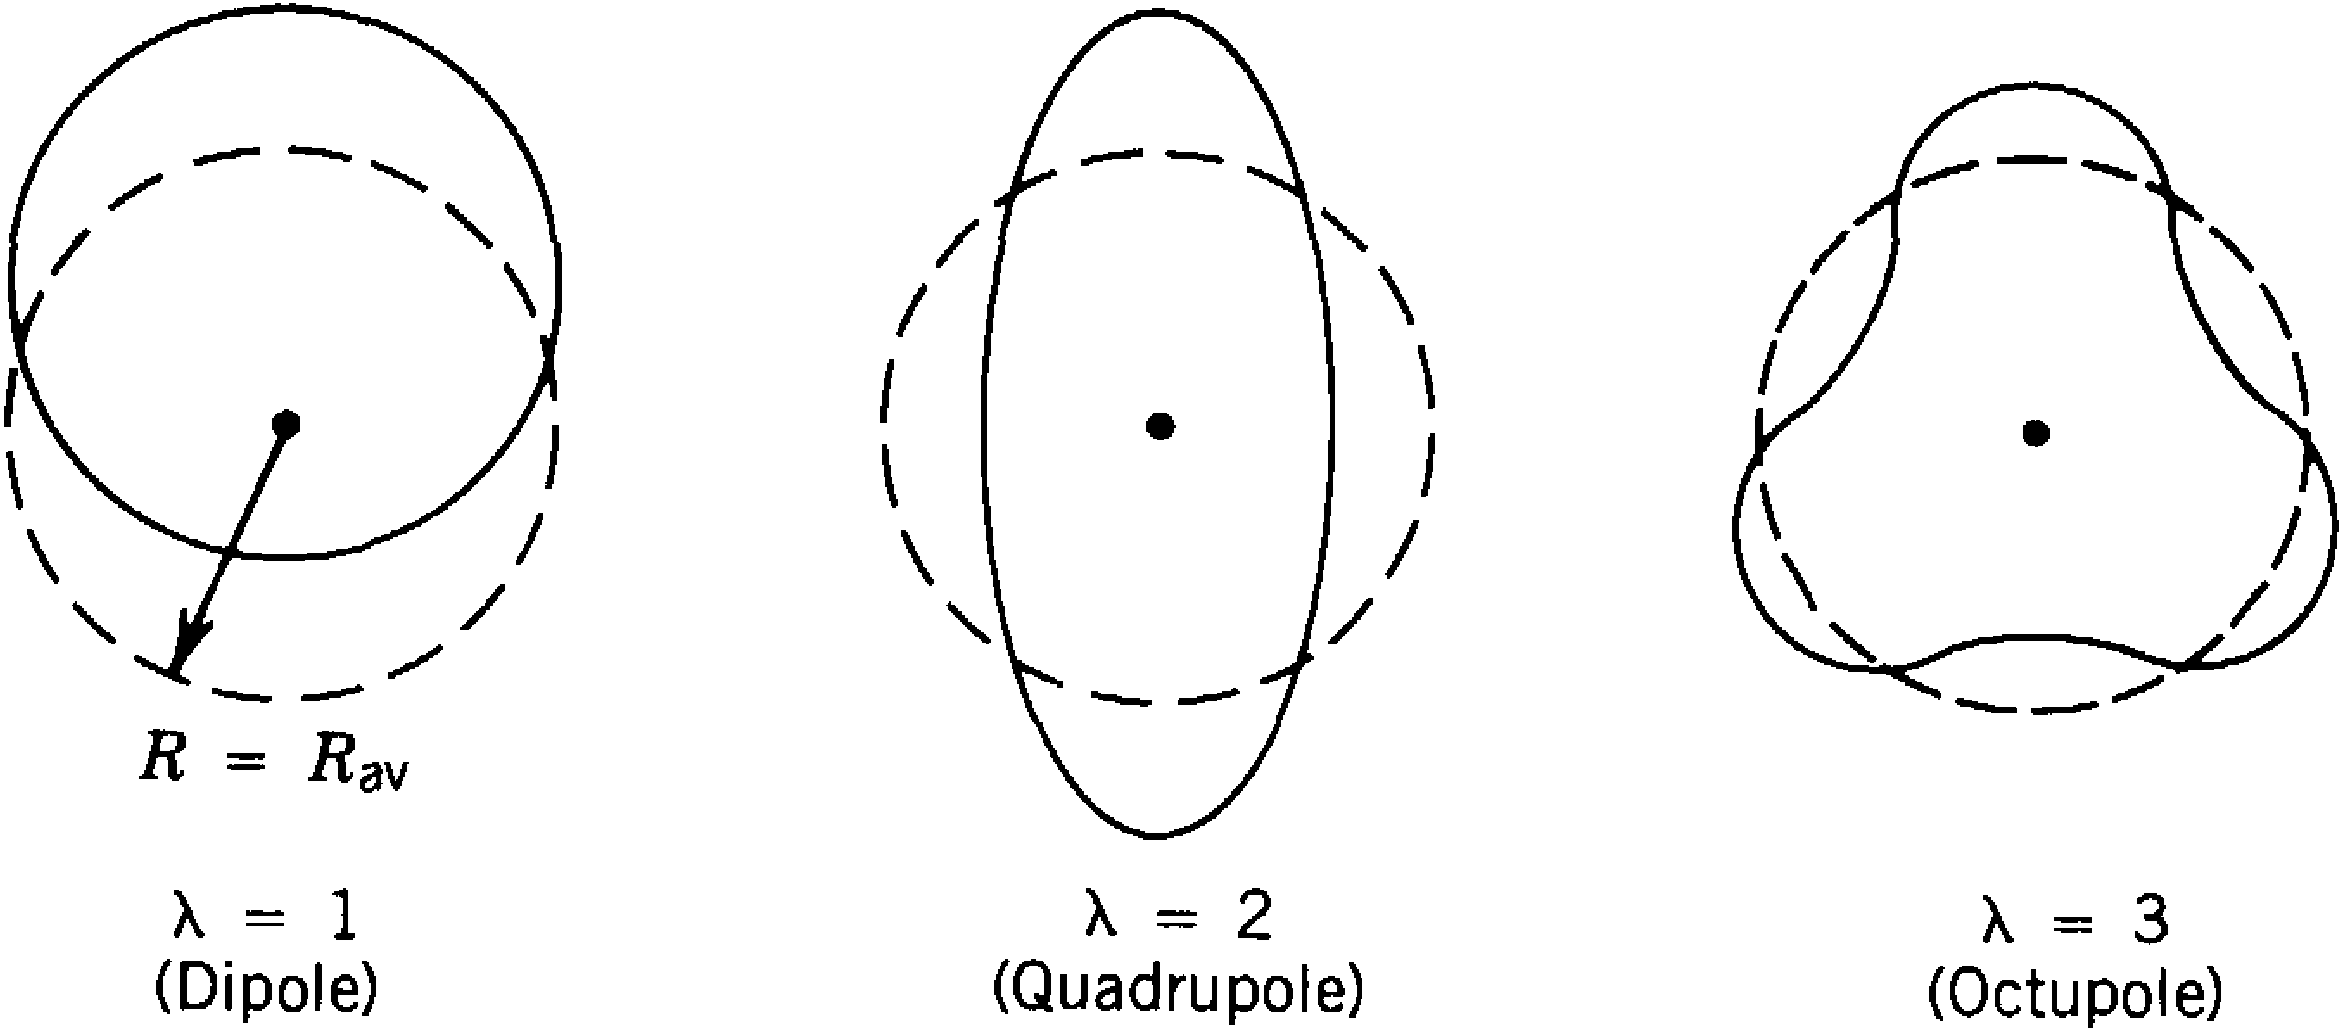
\includegraphics[width = 0.70 \textwidth]{phonons.png}
	\caption{Vibrational phonons.}
	\label{phon}
\end{figure}

Aggiungendo un fonone quadripolare ad un nucleo pari-pari nel suo ground state $ 0^+ $ il momento angolare aumenta di due unità ($ \lambda = 2 $) e la parità resta invariata ($ (-1)^{\lambda} = +1 $), dunque lo stato eccitato è $ 2^+ $: studiandone l'energia, si trova un'andamento sovrapponibile a quello in Fig. \ref{2-p} (l'energia di un fonone non è predetta, ma è un parametro regolabile). Aggiungendo un ulteriore fonone quadripolare, bisogna considerare la composizione dei momenti angolari: ciascun fonone ha 5 componenti $ \mu $, per un totale di 25 combinazioni, ma i fononi hanno funzioni d'onda totali simmetriche (poiché hanno spin intero), dunque le combinazioni si riducono a 15 e corrispondono alle componenti associate a momenti angolari $ \ell = 0,2,4 $. Ci si aspetta dunque di trovare degli stati $ 0^+ $, $ 2^+ $ e $ 4^+ $ a circa il doppio dell'energia del primo stato $ 2^+ $, e ciò e proprio quello che si osserva sperimentalmente: questi non hanno esattamente la stessa energia, confermando che anche questo modello ha le proprie semplificazioni e limitazioni, ma comunque è un'importante prova sperimentale della sua validità. In maniera analoga, si troveranno stati $ 0^+ $, $ 2^+ $, $ 3^+ $, $ 4^+ $ e $ 6^+ $ a circa il triplo dell'energia del primo $ 2^+ $, associati a tre fononi quadripolari, e così via.\\
Per quanto riguarda i fononi ottopolari, essi cambiano la parità dello stato: aggiungengo un fonone ottopolare ad un nucleo pari-pari nel ground state si ottiene uno stato eccitato $ 3^- $, con energia tipicamente superiore al tripletto associato al doppio fonone quadripolare, il quale è anche osservato nei nuclei vibrazionali, a riconferma della validità del modello.

\subsubsection{Giant resonances}
\label{sub-giant-res}

Ad energie superiori iniziano ad influire anche le eccitazioni dovute al pair breaking, dunque la trattazione si fa molto più complessa. Un fenomeno interessante, però, sono le cosiddette \textit{risonanze giganti}: queste vibrazioni avvengono ad energie estremamente elevate ($ > 10\mev $) e coinvolgono praticamente tutti i nucleoni nel nucleo.\\
Le risonanze giganti più importanti sono il monopolo gigante, in cui non c'è trasferimento di momento angolare poiché il nucleo si espande e comprime attorno alla forma sferica, decadendo poi per emissione di particelle, ed il dipolo gigante, in cui invece la distribuzione di protoni e quella di neutroni oscillano in opposizione di fase, decadendo poi per emissione di particelle e raggi $ \gamma $.\\
A livello macroscopico, le risonanze giganti possono essere descritte come le oscillazioni di una goccia attorno ad un punto d'equilibrio, mentre a livello microscopico la trattazione è estremamente difficile ma può essere fornita dal modello a shell: queste risonanze altro non sono che una sovrapposizione coerente di tutte le possibili eccitazioni particle-hole nelle varie shell nucleari, e ciò spiega le alte excitation energies.

\paragraph{Pygmy and Giant Dipole Resonance}

La risonanza vibrazionale più importante e studiata è la risonanza gigante di dipolo (GDR), nella quale tutta la distribuzione di protoni oscilla contro tutta la distribuzione dei neutroni: questo può avvenire sia a seguito dell'assorbimento di un fotone, con la componente elettrica del campo elettromagnetico che causa l'oscillazione dei protoni e lascia inalterati i neutroni, oppure a seguito di reazioni nucleari. Tipicamente si ha $ E_{\text{GDR}} \approx 80\mev \cdot A^{-1/3} $.\\
Va inoltre notato che per nuclei stabilmente deformati i tre assi d'oscillazione non sono ugugali tra loro (solo due lo sono), dunque la tipica forma approssimativamente lorentziana della GDR (vedere Fig. \ref{pgdr}) si va a deformare, fino a presentare due picchi distinti: questo è un importante indicatore di deformazioni permanenti del nuclide.\\
Oltre alla GDR, che coinvolge tutti i nucleoni, nei nuclei neutron-rich è possibile una risonanza di dipolo in cui il core, composto di protoni e neutroni, oscilla rispetto alla neutron skin: questa è detta \textit{Pygmy Dipole Resonance} (PDR), poiché avviene ad energie minori della GDR (vedere Fig. \ref{pgdr}). Si pensa che la PDR diventi estremamente preponderante man mano che si considerano nuclei sempre più esotici e neutron-rich, e ciò ha particolare rilevanza in ambito astrofisico.

\begin{figure}[!t]
	\centering
	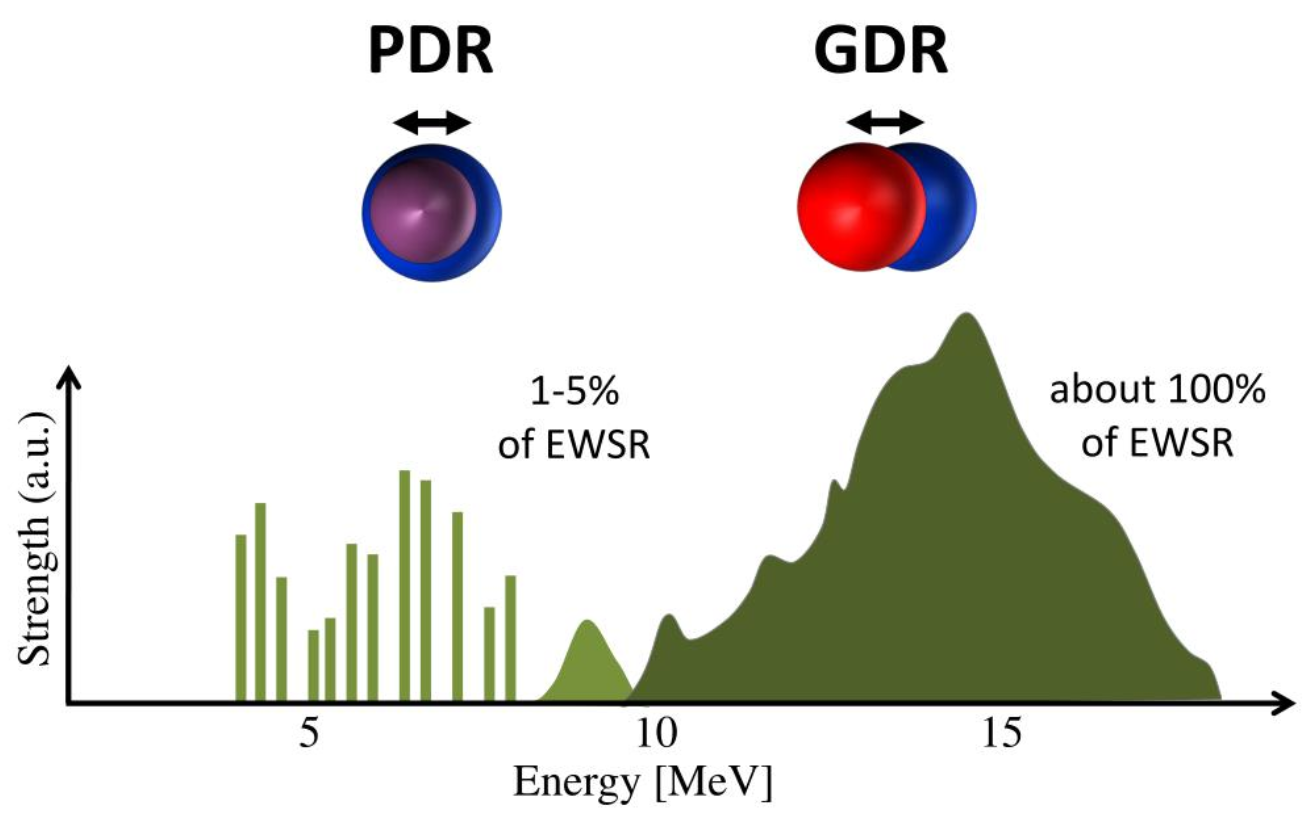
\includegraphics[width = 0.70 \textwidth]{pgdr.png}
	\caption{Pygmy and Giant Dipole Resonances and their respective probabilities.}
	\label{pgdr}
\end{figure}

\subsection{Collective rotations}

Per $ A > 150 $ la forma dei nuclei è stabilmente deformata: gran parte di questi nuclei ha parametro di deformazione (Eq. \ref{eq:5.9}) $ \beta \approx 0.30 $, dunque la differenza tra i due semiassi è circa del 30\%.\\
Dato un corpo rigido di momento d'inerzia $ \mathfrak{I} $ e momento angolare $ I $, l'energia del sistema (tratta quantisticamente) può essere espressa come:
\begin{equation}
	E(I) = \frac{I^2}{2\mathfrak{I}} = \frac{\hbar^2}{2\mathfrak{I}} I (I + 1)
	\label{eq:5.12}
\end{equation}
Nel caso di un nucleo deformato, $ I $ è un quantum number associato al momento angolare totale (sia dei protoni che dei neutroni) e lo spettro energetico così determinato corrisponde ad una serie di stati con $ I $ via via crescente, detta \textit{rotational band}: per un nucleo pari-pari il ground state è $ 0^+ $, quindi la simmetria per riflessione restringe i valori di $ I $ ai soli valori positivi, determinando la rotational band:
\begin{equation*}
	\begin{split}
		E(0^+) &= 0 \\
		E(2^+) &= 6 \frac{\hbar^2}{2\mathfrak{I}} \\
		E(4^+) &= 20 \frac{\hbar^2}{2\mathfrak{I}} \\
		E(6^+) &= 42 \frac{\hbar^2}{2\mathfrak{I}} \\
		       &\vdots
	\end{split}
\end{equation*}
Confrontando coi dati sperimentali, si trova che le energie così calcolate sono leggermente sovrastimate, suggerendo che il nucleo non si comporti propriamente come un corpo rigido. Infatti, modellando il nucleo come un corpo rigido si trova:
\begin{equation}
	\mathfrak{I}_{\text{rigid}} = \frac{2}{5} M \braket{R}^2 (1 + 0.31 \beta)
	\label{eq:5.13}
\end{equation}
Se invece lo si modella come un fluido all'interno di un contenitore ellissoidale:
\begin{equation}
	\mathfrak{I}_{\text{fluid}} = \frac{9}{8\pi} M \braket{R}^2 \beta
	\label{eq:5.14}
\end{equation}
Dai dati sperimentali, si trova che $ \mathfrak{I}_{\text{fluid}} < \mathfrak{I} < \mathfrak{I}_{\text{rigid}} $: il comportamento del nucleo è intermedio tra un corpo rigido, in cui i nucleoni sono fortemente legati tra loro, ed un fluido, in cui invece il legame nucleonico è debole (conseguenza della natura a short-range dell'interazione forte). Una possibile interpretazione per questo fatto è che non tutti i nucleoni partecipano alla rotazione, ma soltanto i nucleoni di valenza al di fuori della shell closure.\\
Va notato che per nuclei deformati è necessario modificare la forma del potenziale nucleare: esso non può più essere a simmetria sferica, ma deve avere il minimo in corrispondenza della deformazione.

\paragraph{Spettro della rotational band}

Sebbene l'energia della rotational band vari quadraticamente col momento angolare (Eq \ref{eq:5.12}), l'energia emessa dalla transizione $ \gamma $ tra due stati eccitati della rotational band varia linearmente con $ I $:
\begin{equation}
	E_{\gamma}(I) \equiv E(I + 2) - E(I) = \frac{2\hbar^2}{\mathfrak{I}} I
	\label{eq:5.15}
\end{equation}
Di conseguenza, lo spettro $ \gamma $ ottenuto con queste transizioni presenta una notevole regolarità, dato che l'energia di tali fotoni è equispaziata:
\begin{equation}
	\Delta E_{\gamma} \equiv E_{\gamma}(I + 2) - E_{\gamma}(I) = \frac{4\hbar^2}{\mathfrak{I}}
	\label{eq:5.16}
\end{equation}
Questo spettro molto regolare è caratteristico della rotational band di nuclei deformati, quindi è un ottimo indicatore per individuare tali nuclei.\\
Inoltre, misurando lo spettro energetico rotazionale, da $ \Delta E_{\gamma} $ si può ottenere una misura di $ \mathfrak{I} $ e dunque di $ \beta $, oltre ad avere una conferma teorica del rapporto costante $ E(4+) / E(2^+) \approx 3.3 $ per nuclei pesanti ($ A > 150 $).

\paragraph{Super-deformed nuclei}

Dagli studi sul momento di quadrupolo anomalo è stata scoperta l'esistenza di nuclidi che presentano delle \textit{super-deformed bands}, ovvero nuclidi con deformazioni estreme (ben oltre $ \beta \approx 0.30 $) che ruotano a velocità incredibili: il primo di questi nuclei ad essere scoperto fu il $ \ch{^{152}Dy} $ nel 1986, con una frequenza di rotazione di $ \sim 10^{21} \,\text{Hz} $. Al giorno d'oggi sono note oltre 350 super-deformed bands.












\chapter{Reazioni Nucleari}
\pagestyle{body}
\selectlanguage{italian}

\section{Proprietà generali}

La forma tipica di una reazione nucleare è la seguente:
\begin{equation*}
	\mathrm{a} + \mathrm{X} \rightarrow \mathrm{Y} + \mathrm{b}
\end{equation*}
dove $ \mathrm{X} $ e $ \mathrm{Y} $ sono nuclidi target-like, $ \mathrm{a} $ e $ \mathrm{b} $ projectile-like. Una scrittura alternativa è: $ \mathrm{X} \left( \mathrm{a},\mathrm{b} \right) \mathrm{Y} $.\\
In linea generale, le reazioni nucleari soddisfano alcune leggi di conservazione, sebbene alcune di esse non in maniera sempre esatta: energia totale, momento lineare totale, momento angolare totale, carica elettrica totale, parità, numero atomico. In base all'energia per nucleone possono presentarsi comportamenti aggiuntivi:
\begin{enumerate}
	\item low-energy ($ E \lesssim 10\mev $ per nucleone): non ci sono processi legati all'interazione forte, dunque si conservano anche il numero di protoni e quello di neutroni;
	\item medium-energy ($ 100\mev \lesssim E \lesssim 1\gev $ per nucleone): subentrano processi di meson production, dunque protoni e neutroni possono trasformarsi gli uni negli altri;
	\item high-energy ($ E \gtrsim 10\gev $ per nucleone); possono essere prodotte molte particelle esotiche, arrivando a riarrangiare anche i quarks nei nucleoni.
\end{enumerate}
Inoltre, dato che affinché avvenga la reazione si deve superare la barriera coulombiana nei nuclei, è necessario che la reazione abbia un certo $ Q $-value. Dalla conservazione dell'energia totale si ha:
\begin{equation*}
	M_{\mathrm{a}} c^2 + T_{\mathrm{a}} + M_{\mathrm{X}} c^2 + T_{\mathrm{X}} = M_{\mathrm{Y}} c^2 + T_{\mathrm{Y}} + M_{\mathrm{b}} c^2 + T_{\mathrm{b}}
	\quad \Rightarrow \quad
	Q = M_{\mathrm{a}} c^2 + M_{\mathrm{X}} c^2 - \left( M_{\mathrm{Y}} c^2 + M_{\mathrm{b}} c^2 \right)
\end{equation*}
Se $ Q > 0 $ si parla di \textit{reazione esoergonica} (o esotermica), nella quale parte della massa nucleare o della binding energy viene liberata sotto forma di energia cinetica, mentre se $ Q < 0 $ di \textit{reazione endoergonica} (o endotermica), nella quale parte dell'energia cinetica è convertita in massa nucleare o binding energy. Nel caso in cui $ Q = 0 $ si parla di \textit{collisione elastica}.\\
Una reazione è sempre possibile se $ Q \ge 0 $, mentre se $ Q < 0 $ è necessario che $ T_{\mathrm{a}} $ superi una certa threshold energy:
\begin{equation}
	T_{\text{th}} = -Q \frac{M_{\mathrm{Y}} + M_{\mathrm{b}}}{M_{\mathrm{Y}} + M_{\mathrm{b}} - M_{\mathrm{a}}}
	\label{eq:6.1}
\end{equation}
Dalla conservazione dell'impulso, invece, considerando il laboratory frame in cui il target $ \mathrm{X} $ è a riposo e definendo $ \theta $ e $ \xi $ gli angoli tra i momenti di $ \mathrm{Y} $ e $ \mathrm{b} $ e quello di $ \mathrm{a} $, si ha:
\begin{equation*}
	\begin{cases}
		p_{\mathrm{a}} = p_{\mathrm{b}} \cos \theta + p_{\mathrm{Y}} \cos \xi \\
		0 = p_{\mathrm{b}} \sin \theta - p_{\mathrm{Y}} \sin \xi
	\end{cases}
\end{equation*}
Si hanno tre equazioni in quattro incognite ($ T_{\mathrm{b}}, T_{\mathrm{Y}}, \theta, \xi $), dunque non c'è soluzione unica. Dato che è più facile osservare $ \mathrm{b} $ rispetto ad $ \mathrm{Y} $, dato che quest'ultimo può rimanere all'interno dello strato target, conviene eliminare le osservabili relative ad $ \mathrm{Y} $, trovando:
\begin{equation}
	\sqrt{T_{\mathrm{b}}} = \frac{1}{M_{\mathrm{Y}} + M_{\mathrm{b}}} \left[ \sqrt{M_{\mathrm{a}} M_{\mathrm{b}} T_{\mathrm{a}}} \cos \theta \pm \sqrt{M_{\mathrm{a}} M_{\mathrm{b}} T_{\mathrm{a}} \cos^2 \theta + \left( M_{\mathrm{Y}} + M_{\mathrm{b}} \right) \left( M_{\mathrm{Y}} Q + (M_{\mathrm{Y}} - M_{\mathrm{a}}) T_{\mathrm{a}} \right)} \right]
	\label{eq:6.2}
\end{equation}
Si può quindi calcolare $ T_{\mathrm{b}} $ in base alla misura dell'angolo $ \theta $.\\
In Fig. \ref{reac-graph} è riportato il plot di $ T_{\mathrm{b}} $ rispetto a $ T_{\mathrm{a}} $ a vari angoli $ \theta $ per la reazione $ \ch{^3H} \left( p,n \right) \ch{^3He} $, la quale ha $ Q = -763.75\kev $: si può notare che quasi ovunque c'è una corrispondenza biunivoca tra $ \theta $ e $ T_{\mathrm{b}} $; fa eccezione una regione tra $ 1.019\mev $ e $ 1.147\mev $, in cui invece per ogni valore di $ \theta $ sono possibili due valori di $ T_{\mathrm{b}} $. In generale, questa double-valued region è presente solo in reazioni con $ Q < 0 $ per $ T_{\text{th}} < T_{\mathrm{a}} < T_{\text{d}} $, con:
\begin{equation}
	T_{\text{d}} = - Q \frac{M_{\mathrm{Y}}}{M_{\mathrm{Y}} - M_{\mathrm{a}}}
	\label{eq:6.3}
\end{equation}

\begin{figure}[!b]
	\centering
	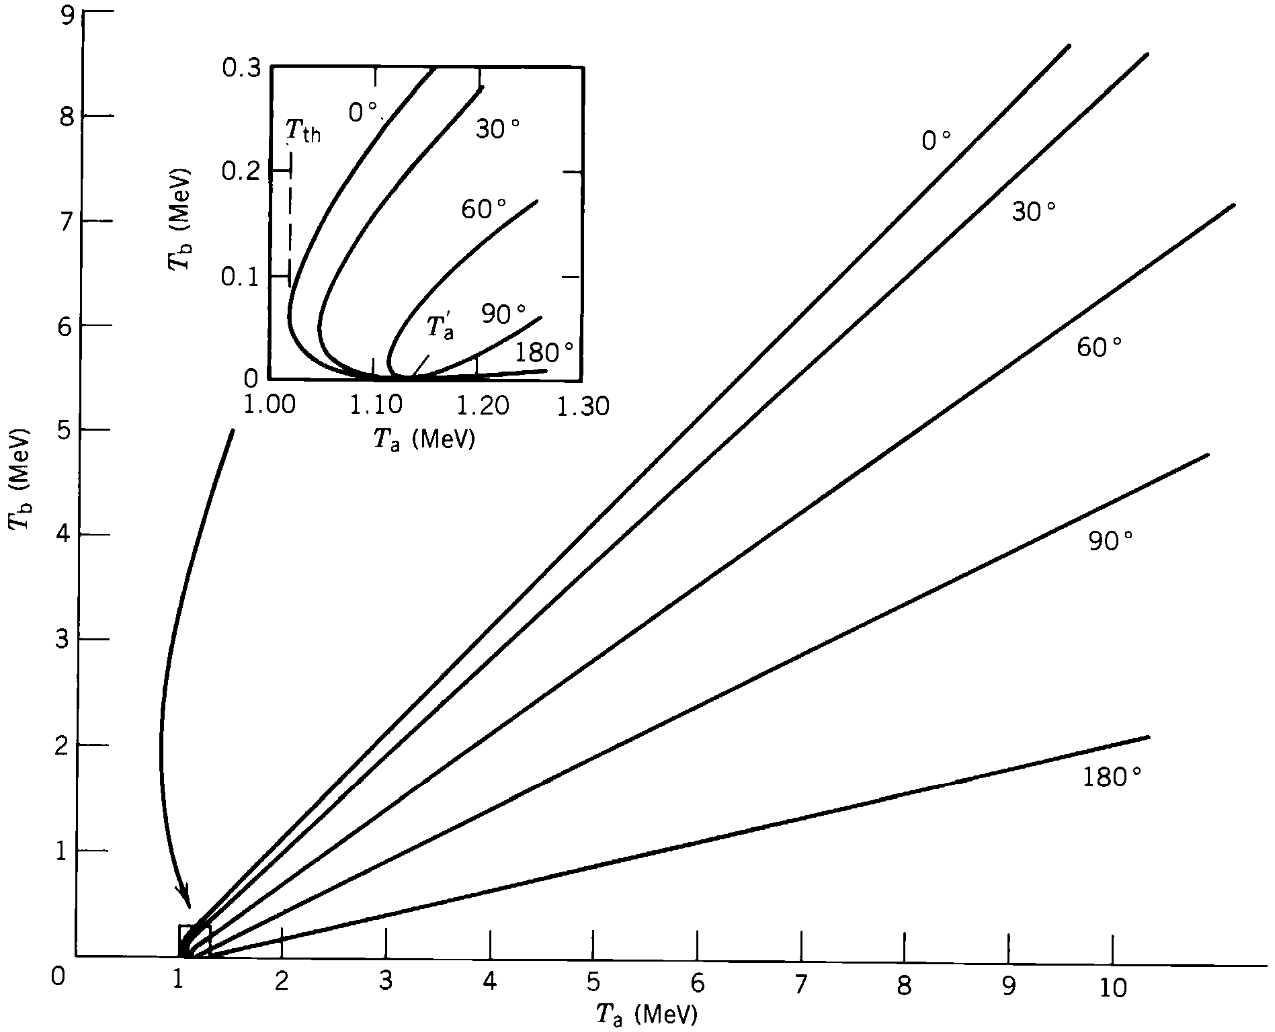
\includegraphics[width=0.70\textwidth]{reac-graph.png}
	\caption{$ T_{\mathrm{b}} $ vs $ T_{\mathrm{b}} $ at various outgoing angles for $ \ch{^3H} \left( p,n \right) \ch{^3He} $.}
	\label{reac-graph}
\end{figure}

\paragraph{Stati eccitati}

È possibile che il nuclide $ \mathrm{Y} $ sia prodotto in uno stato eccitato $ \mathrm{Y}^* $; in tal caso, si vede che il $ Q $-value diminuisce a causa dell'excitation energy $ E_{\text{ex}} $:
\begin{equation}
	Q = Q_0 - E_{\text{ex}}
	\label{eq:6.4}
\end{equation}
dove $ Q_0 $ è relativo alla reazione che produce $ \mathrm{Y} $ nel ground state. È quindi possibile ricostruire lo spettro della specie $ \mathrm{Y} $ calcolando il $ Q $-value a partire da $ T_{\mathrm{a}} $, $ \theta $ (fissati) e $ T_{\mathrm{b}} $ (misurato), il che è possibile invertendo l'Eq. \ref{eq:6.2}:
\begin{equation}
	Q = \left( 1 + \frac{M_{\mathrm{b}}}{M_{\mathrm{Y}}} \right) T_{\mathrm{b}} - \left( 1 - \frac{M_{\mathrm{a}}}{M_{\mathrm{Y}}} \right) T_{\mathrm{a}} - 2 \sqrt{\frac{M_{\mathrm{a}}}{M_{\mathrm{Y}}} \frac{M_{\mathrm{b}}}{M_{\mathrm{Y}}} T_{\mathrm{a}} T_{\mathrm{b}}} \cos \theta
	\label{eq:6.5}
\end{equation}
Solitamente si raggiunge una sufficiente accuratezza utilizzando i numeri atomici al posto delle masse nucleari, specialmente per $ \theta \approx \frac{\pi}{2} $ (si annulla l'ultimo termine).

\paragraph{Cross-section}

Si consideri un projectile beam d'intensità $ \Phi_0 $ (particelle al secondo) diretto su uno strato sottile di nuclei target con spessore $ s $: a causa delle interazioni coi targets, il projectile beam risulta attenuato a seguito del passaggio nello strato sottile, con un'intensità risultante $ \Phi_{\text{f}} $. La frazione di particelle incidenti che reagiscono è funzione della densità numerica di targets $ n_{\text{t}} $ e dalla cross-section $ \sigma $ della reazione:
\begin{equation}
	d\Phi = - \Phi n_{\text{t}} \sigma dx
	\quad \Rightarrow \quad
	\Phi_0 - \Phi_{\text{f}} = \Phi_0 \left( 1 - e^{- n_{\text{t}} \sigma s} \right) \approx \Phi_0 n_{\text{t}} \sigma s
	\label{eq:6.6}
\end{equation}

\paragraph{Trattazione semiclassica}

Classicamente, si può pensare ai nuclidi come sfere rigide che urtano, con vari risultati a seconda del parametro d'impatto $ b $: per $ b \approx R_{\mathrm{X}} $ si ha un urto elastico, per $ b \ll R_{\mathrm{X}} $ ci può essere uno scambio di nucleoni tra i nuclidi, per $ b \approx 0 $ si può arrivare alla formazione di un unico nucleo composto dal nucleo target e da quello incidente.

\section{Reazioni di diffusione e scattering}

Si dicono reazioni di diffusione o di scattering quelle reazioni in cui $ \mathrm{b} = \mathrm{a} $ (o suoi stati eccitati). Si parla di \textit{scattering elastico} per le reazioni $ \mathrm{A} \left( \mathrm{a},\mathrm{a} \right) \mathrm{A} $, di \textit{scattering inelastico} negli altri casi.\\
Lo scattering nucleare elastico presenta delle somiglianze col problema ottico della diffrazione da disco opaco: un nucleo è un forte assorbitore di nucleoni, da cui l'analogia col disco opaco. Come si vede in Fig. \ref{opdisk}, la diffrazione da disco opaco circolare, dunque con bordo ben definito, risulta in un pattern con massimi e minimi approssimativamente equispaziati e d'intensità decrescente, con il primo minimo a $ \theta \approx \frac{\lambda}{R} $ ($ \lambda $ lunghezza d'onda incidente, $ R $ raggio del disco).

\begin{figure}[!b]
	\centering
	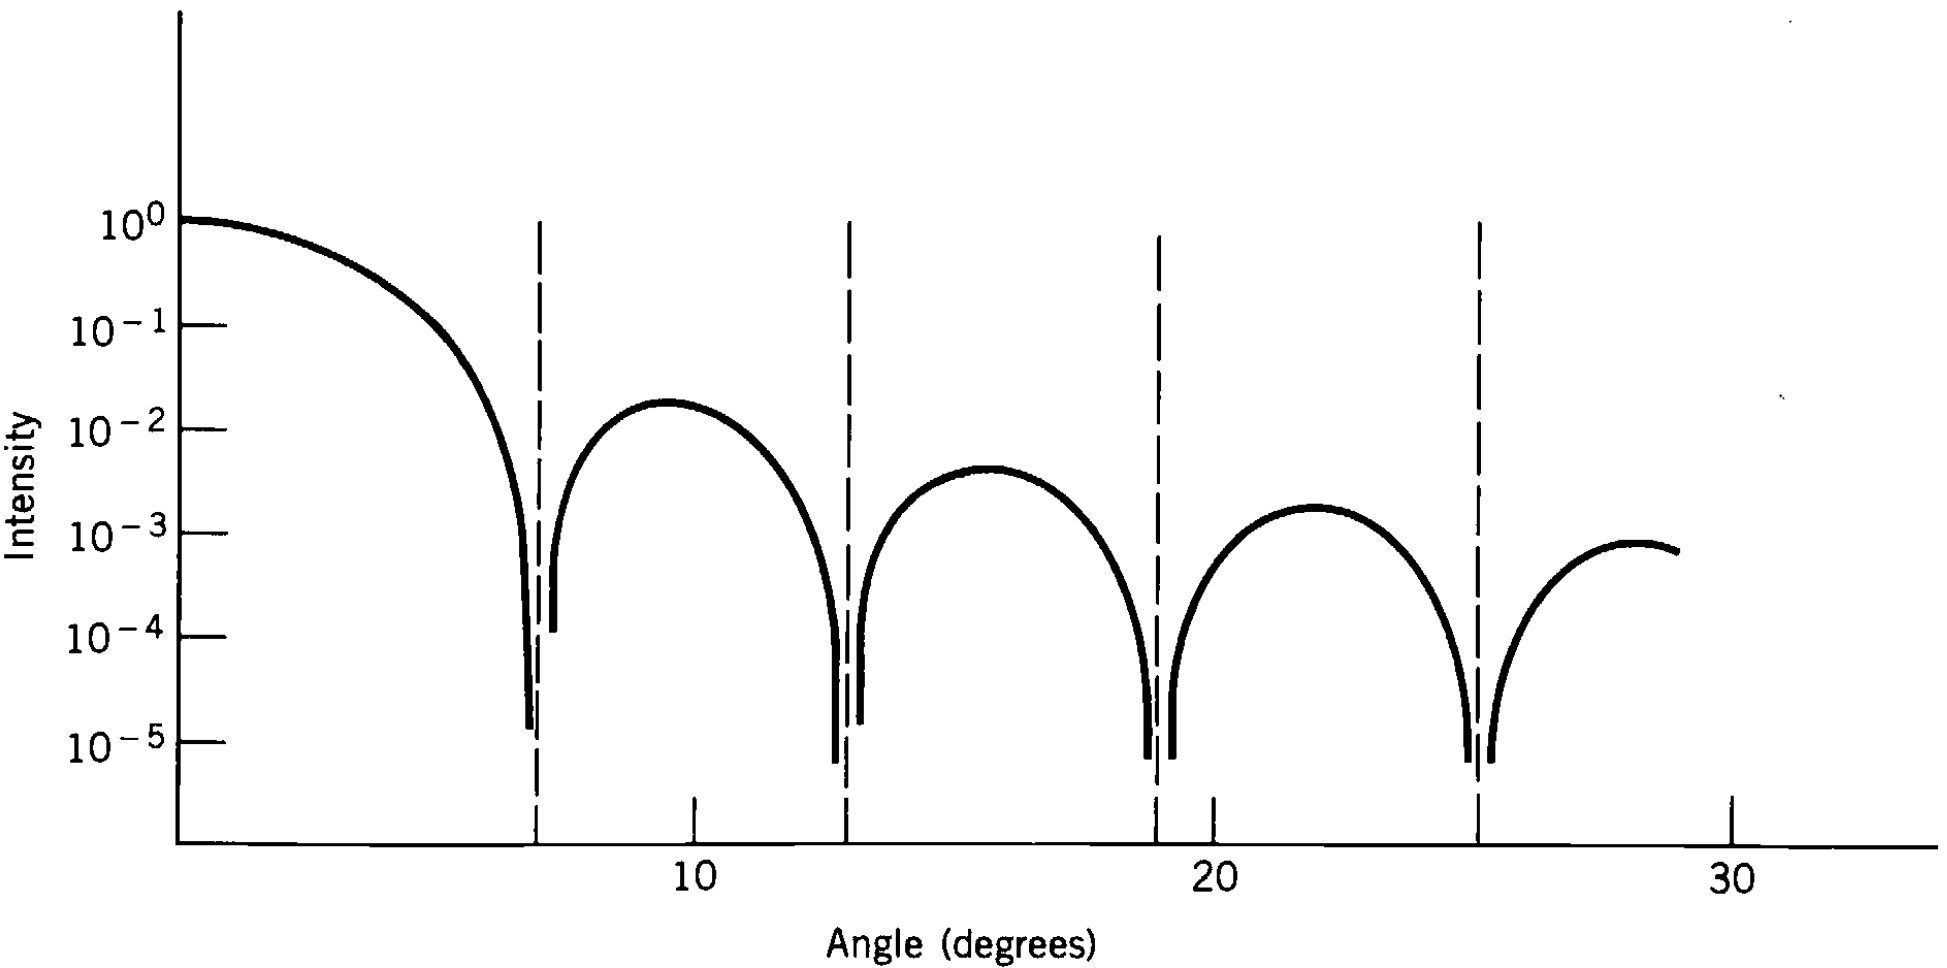
\includegraphics[width=0.70\textwidth]{opdisk.png}
	\caption{Diffraction pattern of light incident on an opaque circular disk.}
	\label{opdisk}
\end{figure}

\begin{figure}[H]
	\centering
	\includegraphics[width=0.70\textwidth]{neutron-scatt.png}
	\caption{Neutron scattering at $ 14\mev $ from $ \ch{^{208}Pb} $.}
	\label{neutron-scatt}
\end{figure}
\begin{figure}[H]
	\centering
	\includegraphics[width=0.70\textwidth]{proton-scatt.png}
	\caption{Proton scattering at $ 14\mev $ from $ \ch{^{208}Pb} $.}
	\label{proton-scatt}
\end{figure}

Nel caso di particelle cariche, si deve considerare la presenza, oltre che dello scattering nucleare, dello scattering coulombiano. Come si vede in Fig. \ref{neutron-scatt}, lo scattering di neutroni, che non subiscono l'interazione coulombiana, segue quasi esattamente il pattern diffrattivo in Fig. \ref{opdisk}, con la differenza che i minimi non vanno a zero dato che la superficie nucleare ha una certa diffusività. Lo scattering di protoni, invece, ha un comportamento diverso: dalla Fig. \ref{proton-scatt} si nota che il comportamento diffrattivo si ha solo per angoli grandi; ad alte energie, invece, l'interazione coulombiana diventa trascurabile.\\
Un'applicazione dello studio dello scattering nucleare è la stima del raggio nucleare: sebbene i valori esatti dipendano dallo specifico potenziale utilizzato per analizzare lo scattering, i risultati sono consistenti con $ R = R_0 A^{1/3} $, con $ R_0 = 1.25\fm $, oltre a mostrare la diffusività della superficie nucleare.

\begin{figure}[!b]
	\centering
	\includegraphics[width=0.75\textwidth]{he-proton-scatt.png}
	\caption{Proton scattering at $ 1050\mev $ from $ \ch{^{208}Pb} $.}
	\label{he-proton-scatt}
\end{figure}

\section{Reazioni dirette ed indirette}

Un'ulteriore classificazione delle reazioni non-scattering è data dalla durata della reazione:
\begin{enumerate}
	\item reazioni dirette, che avvengono in un tempo breve rispetto al tempo di transito del proiettile nel target ($ \sim 10^{-22}\,\text{s} $):
		\begin{itemize}
			\item reazioni di stripping: uno o più nucleoni sono trasferiti dal proiettile al target;
			\item reazioni di pick-up: uno o più nucleoni sono trasferiti dal target al proiettile (es.: $ \left( p,d \right) $, $ \left( n,d \right) $, $ \left( d,\ch{^3H} \right) $, $ \left( d,\ch{^3He} \right) $);
			\item reazioni di knock-out: il proiettile strappa uno o più nucleoni dal target, ma non li assorbe;
		\end{itemize}
	\item reazioni indirette, che avvengono tramite la formazione di uno stato intermedio, detto \textit{nucleo composto}, che dopo un certo tempo decade e produce le particelle finali:
		\begin{itemize}
			\item canale elastico: $ \mathrm{a} + \mathrm{A} \rightarrow \mathrm{C}^* \rightarrow \mathrm{a} + \mathrm{A} $;
			\item canale inelastico: $ \mathrm{a} + \mathrm{A} \rightarrow \mathrm{C}^* \rightarrow \mathrm{a} + \mathrm{B} $;
			\item reazione nucleare: $ \mathrm{a} + \mathrm{A} \rightarrow \mathrm{C}^* \rightarrow \mathrm{b} + \mathrm{B} $;
			\item cattura radiativa: $ \mathrm{a} + \mathrm{A} \rightarrow \mathrm{C}^* \rightarrow \gamma + \mathrm{C} $.
		\end{itemize}
\end{enumerate}
La separazione tra le due classi non è ben definita: in genere, si dicono indirette le reazioni che impiegano più di $ 1\,\mu\text{s} $.\\
Le reazioni dirette avvengono quando la particella incidente è abbastanza energetica da avere una lunghezza d'onda di de Broglie $ \lambda \sim 1\fm $ (es.: un nucleone da $ 20\mev $), interagendo dunque con singoli nucleoni alla periferia del nucleo: si parla infatti di \textit{peripheral processes}. La particella risultante è generalmente emessa in avanti, ovvero ad angoli piccoli rispetto alla direzione della particella incidente.

\subsection{Reazioni di stripping}

Le reazioni di stripping più semplici sono quelle indotte dal deuterio $ d \equiv \ch{^2H} $ (binding energy $ 2.2\mev $):
\begin{equation*}
	d + \ch{X}(A,Z) \rightarrow p + \ch{X}(A+1,Z)
	\qquad \qquad
	d + \ch{X}(A,Z) \rightarrow n + \ch{X}(A+1,Z+1)
\end{equation*}
È possibile trattare in maniera semiclassica tale reazione, ignorando gli spin delle particelle. Si consideri una particella incidente con momento $ \ve{p}_a $ che determina una particella in uscita di momento $ \ve{p}_b $: il nucleo residuale, composto dal nucleo iniziale più il nucleone scambiato, ha quindi un momento di recoil $ \ve{p} = \ve{p}_a - \ve{p}_b $. In un processo diretto è possibile assumere che il trasferimento di momento sia istantaneo e che il nucleone scambiato venga posto in un orbitale nucleare con $ \ell \approx \frac{1}{\hbar} Rp $, dove $ R $ è il raggio del nuclide (peripheral process):
\begin{equation*}
	p^2 = p_a^2 + p_b^2 - 2 p_a p_b \cos \theta = \left( p_a - p_b \right)^2 + 2 p_a p_b \left( 1 - \cos \theta \right)
\end{equation*}
Assumendo $ p_a \approx p_b \equiv p_0 $, si trova:
\begin{equation}
	\ell = \frac{2}{\hbar} R p_0 \sin \frac{\theta}{2}
	\label{eq:6.7}
\end{equation}
Ad esempio, si consideri la reazione $ \ch{^{90}Zr} \left( d,p \right) \ch{^{91}Zr} $: essa ha $ Q = 5\mev $, dunque un deuterone incidente di $ 5\mev $ produce un protone in uscita di $ 10\mev $, al meno di eccitazioni di $ \ch{^{91}Zr} $.
Come si vede in Fig. \ref{zr-spec}, i picchi nello spettro di protoni della reazione identificano vari stati eccitati del $ \ch{^{91}Zr} $ che vengono popolati dalla reazione. Dallo studio degli angoli a cui vengono emessi i protoni (Fig. \ref{zr-ang}), ed in particolare dei massimi della distribuzione angolare di protoni, si posso determinare i numeri quantici $ \ell $ dei neutroni trasferiti e, di conseguenza, delle shell che essi occupano nei vari stati eccitati.

\begin{figure}[H]
	\centering
	\includegraphics[width=0.75\textwidth]{zr-spec.png}
	\caption{Proton spectrum from $ \ch{^{90}Zr} \left( d,p \right) \ch{^{91}Zr} $.}
	\label{zr-spec}
\end{figure}

\begin{figure}[H]
	\centering
	\includegraphics[width=0.60\textwidth, angle=90]{zr-ang.png}
	\caption{Angular distributions for $ \ch{^{90}Zr} \left( d,p \right) \ch{^{91}Zr} $.}
	\label{zr-ang}
\end{figure}

\subsection{Reazioni di nucleo composto}

Si consideri una particella proiettile che penetra il nucleo target con un parametro d'impatto piccolo rispetto al raggio nucleare: ciò genera una serie di collisioni interne al nucleo composto così formato, con un conseguente aumento dell'energia media per nucleone. Le collisioni random che avvengono all'interno del nucleo ripartiscono l'energia incidente tra tutti i nucleoni del sistema proiettile+target secondo una certa distribuzione statistica di energia, dunque c'è una certa probabilità che un nucleone accumuli abbastanza energia per fuggire dal potenziale nucleare, in maniera equivalente ad una molecola in un liquido in evaporazione. Data la natura casuale delle collisioni nel nucleo, le particelle così emesse sono distribuite isotropicamente nello spazio (a differenza delle reazioni dirette che emettono tendenzialmente in avanti) e la loro energia è distribuita secondo una distribuzione maxwelliana.\\
Si vede dunque che le reazioni di nucleo composto possono essere divise in due step: la formazione del nucleo composto ed il suo successivo decadimento, il quale può avere vari decay modes con meccanismi diversi. L'assunzione fondamentale, confermata dai dati sperimentali, è che la probabilità relativa di un certo decay mode è indipendente da come si è formato il nucleo composto, ma determinata soltanto dall'energia totale del sistema.\\
Il modello a nucleo composto funziona bene per proiettili a bassa energia, che hanno una bassa probabilità di fuoriuscire dal nucleo senza subire cambiamenti e senza cessioni di energia, e per target medi e pesanti, che hanno una struttura nucleare abbastanza grande da assorbire tutta l'energia incidente.

\section{Reazioni fotonucleari}

L'analisi dettagliata delle reazioni indotte dai fotoni sui nuclei permette di studiare le eccitazioni collettive di molti nucleoni, andando oltre i modelli di particella singola: queste sono spiegate fenomenologicamente come fluttuazioni di forma o densità del sistema many-body attorno ad uno stato d'equilibrio.\\
La produzione di raggi $ \gamma $ monocromatici è possibile grazie a sorgenti radioattive (es.: $ \ch{^{24}Na} $ e $ \ch{^{60}Co} $, con $ E_{\gamma} \approx 1-3\mev $) e fasci protonici incidenti su litio ($ p + \ch{Li} $ produce raggi $ \gamma $ con $ E_{\gamma} \approx 17\mev $); sorgenti di raggi $ \gamma $ ad energia variabile sono invece basate sull'annichilazione di positroni.\\
Con i fasci ad enegia variabile sono stati ottenuti risultati di precisione sia sulla sezione d'urto totale dell'assorbimento di un fotone dal nucleo, sia sulla \textit{fotoproduzione di neutroni}:
\begin{equation*}
	\gamma + \ch{X}(A,Z)\rightarrow n + \ch{X}(A-1,Z)
\end{equation*}
Questa reazione rappresenta la maggior parte della sezione d'urto totale, dato che la fotoproduzione di protoni è sfavorita dalla barriera coulombiana.

\paragraph{Giant Dipole Resonance}

La cross-section da assorbimento di fotoni è dominata da un'ampia risonanza, nota come \textit{Giant Dipole Resonance} (GDR). Ad esempio, si consideri la cross-section per la fotoproduzione di neutroni da isotopi di \ch{Nd}, riportata in Fig. \ref{gdr-nd}: si vede che la sezione d'urto presenta un massimo per $ E_{\gamma} \approx 15\mev $ ed un andamento a risonanza abbastanza larga. La GDR è osservata per moltissimi nuclei, da quelli leggeri come $ \ch{^3He} $ a quelli pesanti come $ \ch{^{232}Th} $; per nuclei medi e pesanti, l'energia di eccitazione della risonanza può essere stimata come $ E_{\text{GDR}} \approx A^{-1/3} \cdot 80\mev $.

\begin{figure}
	\centering
	\includegraphics[width=0.70\textwidth]{gdr.png}
	\caption{Cross-section for $ \gamma $-induced emission of neutrons in neodymium isotopes.}
	\label{gdr-nd}
\end{figure}











\part{Fisica Subnucleare}
\pagestyle{body}

\chapter{Fisica delle Particelle}
\selectlanguage{italian}

La fisica delle particelle studia i costituenti fondamentali della materia e le interazioni fra loro. La materia è costituita da particelle e campi, i quali sono associati alle interazioni e causano le forze attraverso le quali interagiscono le particelle: le interazioni sono mediate da particolari particelle, dette \textit{bosoni di gauge}. Le particelle fondamentali, come i quarks e l'elettrone, possono essere considerati puntiformi ($ \lesssim 10^{-16}\,\text{cm} $, mentre un nuclide $ \sim 10^{-13}\,\text{cm} $).

\paragraph{Particelle}

Solo quattro particelle sono stabili, di cui sono due sono fondamentali: il protone, il neutrone, l'elettrone ed il neutrino. Le altre particelle decadono rapidamente verso le particelle stabili, ed infatti sono tendenzialmente più massive di quest'ultime. A causa dell'instabilità, queste particelle non si trovano in natura, ma possono essere prodotte sperimentalmente usando fasci di particelle incidenti con sufficiente energia (superiore alla rest energy delle particelle da produrre).\\
Attualmente, le particelle fondamentali più massive scoperte sono il bosone $ W $ ($ 80.4\gev/c^2 $), il bosone $ Z $ ($ 91.2\gev/c^2 $), il bosone di Higgs ($ 125\gev/c^2 $) ed il quark top ($ 173\gev/c^2 $). Ciascuna di queste particelle è circa un centinaio di volte più pesante del protone; per produrle sono necessarie altissime energie, mentre per studiarle è necessario sondare distanze piccolissime: dal principio di Heisenberg, se $ \Delta x \ll 1\fm $, allora $ \Delta p \gg 200\mev/c $.

\paragraph{Interazioni}

Tutte le interazioni tra particelle sono dovute allo scambio di particelle mediatrici. Ad oggi si conoscono solo quattro interazioni fondamentali: quella gravitazionale, quella debole, quella elettromagnetica e quella forte. Si pensa, però, che nelle prime frazioni di secondo dell'universo queste fossero unificate (almeno quelle forte, debole ed elettromagnetica): si parla di \textit{Grand Unification Theory} (GUT), secondo la quale, col trascorrere del tempo ed il diminuire della temperatura dell'universo, le interazioni si siano gradualmente separate, fino ad avere quelle che osserviamo oggi. Le predizioni della GUT, però, rimangono tuttora inosservate sperimentalmente: le principali sono il decadimento del protone su scale lunghissime, l'esistenza di monopoli magnetici e l'esistenza di dipoli elettrici fondamentali, ovvero particelle che, sebbene puntiformi, presentano un'asimmetria di carica.

\paragraph{Modello Standard}

All'inizio del Novecento si avevano evidenze sperimentali soltanto dell'elettrone, del fotone e dei nuclei atomici, ma nel giro di un secolo si è arrivati a sviluppare un modello che spiegasse la formazione di tutte le particelle della materia a partire da quelle fondamentali: il \textit{Modello Standard} (Fig. \ref{standard-model}). Questo è appunto un modello, e non una teoria: mentre la seconda dà spiegazioni esatte dei dati sperimentali e ne predice di nuovi, un modello è soltanto un'approssimazione desunta dagli esperimenti, dunque deve essere integrato man mano che questi procedono, e non ha potere predittivo. Il Modello Standard è uno dei modelli più solidi mai sviluppati e ad oggi non è stato ancora messo in crisi, sebbene non spieghi varie cose: ad esempio, la massa dei neutrini e la divisione dei fermioni in generazioni.

\begin{figure}
	\centering
	\includegraphics[width=0.70\textwidth]{standard-model.jpg}
	\caption{Standard Model of particle physics.}
	\label{standard-model}
\end{figure}

\section{Antimateria}

Una delle caratteristiche fondamentali delle particelle, lo spin (momento angolare intrinseco), permette di distinguerle in due classi: i bosoni, con spin intero, ed i fermioni, con spin semi-intero. I fermioni rispondono al principio d'esclusione di Pauli, il quale postula che non ci possono essere due fermioni occupanti lo stesso stato quantistico, mentre ciò è possibile per i bosoni: questo dà luce a fenomeni particolari come la superconduttività e la superliquidità.\\
Se si ignora lo spin, l'equazione di Schrödinger può essere facilmente espressa in forma relativistica; partendo dall'energia $ E^2 = m^2 c^4 + p^2 c^2 $ e ricordando le regole di quantizzazione $ E \mapsto i\hbar \frac{\pa}{\pa t}, p \mapsto -i\hbar \nabla $, si ottiene l'\textit{equazione di Klein-Gordon}:
\begin{equation}
	\frac{1}{c^2} \frac{\pa^2}{\pa t^2} \phi(\ve{x},t) - \lap \phi(\ve{x},t) + \frac{m^2 c^2}{\hbar^2} \phi(\ve{x},t) = 0
	\label{eq:7.1}
\end{equation}
dove $ \phi(\ve{x},t) $ è un campo scalare. Per trattare particelle dotate di spin, è necessario trovare altre equazioni. Per particelle con $ s = \frac{1}{2} $, descritte da uno spinore $ \psi $ a quattro componenti, si trova l'\textit{equazione di Dirac}:
\begin{equation}
	i \gamma^{\mu} \pa_{\mu} \psi - \frac{mc}{\hbar} \psi = 0
	\label{eq:7.2}
\end{equation}
dove le matrici $ \gamma $ sono legate alle matrici di Pauli:
\begin{equation*}
	\gamma^0 \equiv
	\begin{bmatrix}
		\tens{I}_2 & 0 \\ 0 & \tens{I}_2
	\end{bmatrix}
	\qquad \qquad
	\gamma^k \equiv
	\begin{bmatrix}
		0 & \sigma_k \\ -\sigma_k & 0
	\end{bmatrix}
\end{equation*}
La prima grande conseguenza dell'equazione di Dirac è che, risolvendola per elettroni liberi, si trovano due soluzioni: una con energia positiva ed una con energia negativa. Dato che nel mondo reale tutte le energie sono positive, essendoci un'energia minima per le particelle costituita dalla loro massa a riposo, Dirac spiegò la soluzione ad energia negativa tramite l'idea del \textit{Fermi sea}: oltre agli stati ad energia positiva, esistono anche stati speculari ad energia negativa che sono normalmente tutti occupati, così che le particelle reali possano avere solo energie positive. Può capitare però che, con eccitazioni sufficientemente energetiche, una particella nel mare di Fermi venga portata in uno stato ad energia positiva: il vuoto lasciato nel mare di Fermi è interpretato come una antiparticella, ovvero come una copia della particella reale ma con carica elettrica opposta. Questo è proprio il principio della pair production: un fotone sufficientemente energetico ($ E_{\gamma} > 2m_e = 1022\kev $) può fornire l'eccitazione sufficiente a produrre una coppia elettrone-positrone.\\
Un'interpretazione diversa dell'antimateria sarà poi data da Feynman: le antiparticelle non sono più viste come buchi nel Fermi sea, ma come particelle che si muovono in maniera opposta lungo la direzione temporale: ciò comporta che le antiparticelle hanno la stessa massa delle particelle, ma carica elettrica opposta.

\subsection{Evidenze sperimentali}

Le prime evidenze sperimentali dell'esistenza dell'antimateria si ebbero con lastre fotografiche che, mostrando tracce di ionizzazione, rilevavano fenomeni di pair production.

\paragraph{Positrone}

Il positrone fu osservato per la prima volta da Skobeltsyn nel 1929 durante lo studio di raggi cosmici in una cloud chamber e nel 1932 da Anderson con lo stesso metodo. La scoperta fu confermata nel 1932 da Blacket ed Occhialini in laboratorio. A posteriori, altri sperimentatori in precedenza si sarebbero potuti accorgere della sua esistenza: ad esempio, i coniugi Curie lo avevano osservato, ma senza dargli attenzione lo avevano classificato come un protone.\\
Il positrone è una particella stabile come l'elettrone, ma la sua vita media è comunque estremamente breve ($ \tau \sim 10^{-10}\,\text{s} $) poiché forma immediatamente un sistema con un elettrone nella materia, detto positronio, il quale decade per annichilazione.\\
Un'importante applicazione del positrone è la \textit{Positron-Electron Tomography} (PET), un esame diagnostico per tumori: dato che il positronio decade in due fotoni con $ E_{\gamma} = 511\kev $ emessi in direzioni opposte, facendo accumulare una concentrazione abbastanza alta di un positron-emitting radionuclide in una massa tumorale, è possibile tracciarne con precisione la posizione nel corpo, dato che essa deve trovarsi lungo la linea che congiunge i due fotoni rilevati. Un metodo utilizzato è l'accumulo di $ \ch{^{18}F} $ (decade $ \beta^+ $) misto a glucosio: le cellule tumorali hanno un consumo di zuccheri dieci volte superiore alle cellule normali.

\paragraph{Antiprotone}

L'antiprotone fu osservato nel 1955 al Bevatron, un sincrotrone per protoni a Berkley, da Chamberlain e Segrè: ciò confermò che ogni particella aveva una corrispondente antiparticella identica ad essa ma di carica elettrica opposta. Il delay di 20 anni tra le due scoperte fu dovuto al fatto che la massa del protone è quasi 2000 volte quella dell'elettrone, dunque anche le energie necessarie alla produzione di antiprotoni lo sono.\\
Anche gli antiprotoni sono stabili ma short-lived, sempre a causa dell'annichilimento da contatto con materia ordinaria.\\
Poco dopo la conferma dell'esistenza dell'antiprotone, nel 1956 sempre al Bevatron fu osservato l'antineutrone.



\chapter{Leptoni}
\selectlanguage{italian}

I leptoni sono le particelle fondamentali più leggere, se comparate ai sistemi formati da quarks (mesoni e barioni); fa eccezione il tauone ($ 1.78\gev/c^2 $). Sono divisi in tre generazioni, detti anche flavours, ciascuna composta da una particella di carica elettrica $ q = -1e $ ed un neutrino elettricamente neutro; inoltre, i leptoni non sono soggeti all'interazione forte.

\section{Raggi cosmici}

I \textit{raggi cosmici} (o astroparticelle) sono particelle o gruppi di particelle ad alte energie che si muovono nello spazio a velocità relativistiche: principalmente si tratta di protoni e nuclei atomici. Essi possono avere origine solare, galattica o anche extragalattica.\\
All'impatto con l'atmosfera, i raggi cosmici producono delle \textit{showers} di patricelle secondarie a causa dell'interazione con le molecole atmosferiche: parte di queste showers riesce ad arrivare sulla superficie terrestre, risultando dunque rilevabile a terra, mentre la maggior parte viene deflessa nello spazio dalla magnetosfera.\\
Lo studio approfondito dei raggi cosmici è importante principalmente perché costituiscono una fonte di pericolo per missioni spaziali ed extraplanetarie: essi causano danni ai sistemi elettronici e biologici non protetti da un'atmosfera o una magnetosfera, dunque sono una complicazione  per missioni lunari e marziane. In maniera non secondaria, gli ultra-high-energy cosmic rays (UHECRs) possono raggiungere energie fino a $ 3\cdot10^{20}\ev $ (massimo finora osservato), di svariati ordini di grandezza superiori a quelle raggiungibili negli accelleratori odierni: si parla infatti di accelleratori cosmici.

\subsection{Osservazioni}

Le prime osservazioni di raggi cosmici furono svolte da Hess et al. nel 1912 con un pallone aerostatico: misurando la radiazione inonizzante in funzione dell'altezza, si scoprì che essa aumentava man mano che si allontanava dalla superficie terrestre. La conclusione fu che la sorgente di questa radiazione doveva essere extraplanetaria: la causa della ionizzazione dell'atmosfera sono appunto i raggi cosmici. La maggior parte della radiazione dovuta ai raggi cosmici è assorbita dall'atmosfera o deflessa nello spazio, ma una parte riesce ad arrivare alla superficie terrestre.

\subsubsection{Primary Cosmic Rays}

I raggi cosmici primari sono quelli che collidono direttamente con l'atmosfera terrestre: sono costituiti principalmente da protoni e raggi $ \alpha $ (nuclei di idrogeno ed elio), ma una frazione relativamente piccola è costituita dai cosiddetti \textit{ioni HZE} (high atomic number and energy), i quali sono nuclei di atomi pesanti ($ Z > 2 $) con cariche elettriche maggiori di $ +3e $. Quest'ultimi sono particolarmente pericolosi per i cosmonauti, poiché contribuiscono in maniera significativa alla loro dose assorbita di radiazione.\\
In Fig. \ref{flux-cr} è riportato il flusso incidente di di raggi cosmici: si può vedere che l'andamento non è liscio ma presenta tre picchi, detti knees ed ankle: si pensa che i due knees siano dovuti al fatto che gli accelleratori di raggi cosmici galattici abbiamo un massimo energetico oltre il quale non possono accellerare particelle, mentre l'ankle dovrebbe corrispondere ad una zona dominata dai raggi cosmici extragalattici, sebbene ci sia ancora molta incertezza su questi dati.

\begin{figure}
	\centering
	\includegraphics[width=0.70\textwidth]{cosmic-rays.png}
	\caption{Flux of cosmic rays.}
	\label{flux-cr}
\end{figure}

\subsubsection{Secondary Cosmic Rays}

Interagendo con le molecole nell'atmosfera, i raggi cosmici primari producono showers di particelle, dette raggi cosmici secondari: questi sono principalmente pioni, ma una frazione minore è composta da kaoni, protoni, neutroni e rispettive antiparticelle. La componente mesonica (pioni e kaoni) decade principalmente producendo muoni e neutrini:

\begin{equation*}
	\pi^0 \rightarrow \gamma + \gamma \qquad \pi^+ \rightarrow \mu^+ + \bar{\nu}_{\mu} \qquad \pi^- \rightarrow \mu^- + \nu_{\mu}
\end{equation*}
\begin{equation*}
	K^{\pm} \rightarrow \pi^{\pm} + \pi^0 \qquad K^+ \rightarrow \pi^+ + \bar{\nu}_{\mu} \qquad K^- \rightarrow \mu^- + \nu_{\mu}
\end{equation*}

Importanti studi sui raggi cosmici secondari sono stati svolti da Bruno Rossi: nel 1932, si accorse della presenza di due componenti nelle showers, un \textit{soft component} ed un \textit{hard component}. Il soft component, circa il 30\% della radiazione secondaria, è costituita dalle electromagnetic showers, dovute principalmente al decadimento del $ \pi^0 $ e costituite da coppie elettrone-positrone e fotoni ad alta energia: il nome è dovuto al fatto che queste particelle vengono bloccate da pochi millimetri di materiale assorbente. L'hard component, invece, costituisce il 70\% della radiazione secondaria ed è costituito dalle hardonic showers: queste comprendono princiaplmente muoni e, se sufficientemente energetici, possono penetrare vari metri di materiale assorbente.

\paragraph{Pierre Auger Observatory}

Il Pierre Auger Observatory è un osservatorio internazionale di raggi cosmici secondari situato in Argentina: il suo obbiettivo è la rilevazione di UHECRs con energie $ \gtrsim 10^18\ev $. Questi hanno un flusso stimato di $ 1\,\text{km}^{-2} / 100\,\text{y} $, dunque è necessaria una vasta area d'osservazione: essendo composto da 200 water tanks con detection area di $ 12\,\text{km}^2 $, il PAO ha una detection area complessiva di oltre $ 3000\,\text{km}^2 $, comparabile alla superficie del Lussemburgo.\\
In particolare, l'osservazione precisa delle showers da parte di numerose water tanks permette di estrapolare informazioni sulla direzione del cosmic ray e sulla posizione approssimativa della sua sorgente.

\subsection{Muoni}

Il muone è stata la prima particella fondamentale instabile scoperta: esso ha $ m_{\mu} = 105.7\mev/c^2 $, $ \tau = 2.196\,\mu\text{s} $, $ q = -1e $ e $ s = \frac{1}{2} $. Inizialmete si era pensato che fosse il mesone di Yukawa, ovvero il mediatore dell'interazione forte (all'epoca detto mesotrone), ma studiando il suo decadimento si notò che non c'erano legami tra il muone ed i nucleoni:
\begin{equation*}
	\mu^- \rightarrow e^- + \bar{\nu}_e + \nu_{\mu}
\end{equation*}
Questo è un esempio di conservazione del numero leptonico: a ciascuna famiglia leptonica è associato un numero leptonico, il quale deve essere conservato nei decadimenti: ai leptoni è associato $ +1 $, mentre agli antileptoni $ -1 $, dunque nel decadimento del muone devono rimanere costanti $ L_e = 0 $ ed $ L_{\mu} = +1 $, ergo la presenza di $ \bar{\nu}_e $ e $ \nu_{\mu} $.\\
Il muone costituisce anche un perfetto esempio di cinematica relativistica: assumendo che vengano prodotti muoni a $ 10\,\text{km} $ dalla superficie terrestre a causa di raggi cosmici e che essi si muovano a velocità $ 0.98c $, essi impiegherebbero $ t = 34\,\mu\text{s} $ per arrivare a terra; data la vita media del muone $ t_{1/2} = 1.56\,\mu\text{s} $, a terra dovrebbe giungere una frazione del flusso iniziale pari a $ 2^{-34/1.56} = 0.27\cdot10^{-6} $, praticamente nulla. Non si sta però contando la dilatazione relativistica dei tempi: per il muone $ \gamma \approx 5 $, dunque la vita media nel suo rest-frame è sempre $ 1.56\,\mu\text{s} $, ma per un osservatore a riposo rispetto alla Terra essa è $ t'_{1/2} = \gamma t_{1/2} = 7.8\,\mu\text{s} $: la frazione di flusso osservata nel frame della Terra è quindi $ 0.049 $, che è quella effettivamente misurata. ALternativamente, si può anche svolgere il calcolo nel rest-frame dei muoni, considerando dunque la contrazione delle lunghezze: nel loro frame, i muoni non percorrono $ 10\,\text{km} $, bensì $ 2\,\text{km} $.\\
I muoni costituiscono la principale fonte di rumore nella misura degli eventi rari a terra, con un flusso medio al livello del mare di $ 1\,\text{cm}^{-2} / \text{min} $: una soluzione per l'eliminazione del muon background è quella di costruire laboratori sotterranei, specialmente sotto montagne rocciose alte (es.: il Gran Sasso).

\paragraph{Scoperta}

Nel 1936 Anderson e Neddermeyer, studiando la radiazione cosmica al Caltech, si accorsero di particelle che, in presenza di un campo magnetico, curvavano in maniera simile agli elettroni ma con raggio diverso: in particolare, la curva era più larga di quella degli elettroni, ma più stretta di quella dei protoni, dunque si evinse l'esistenza di una particella simile all'elettrone ma con massa intermedia tra quella dell'elettrone e quella del fotone.\\
Per quanto riguarda invece la misura della vita media del muone, il principale limite è posto dagli effetti relativistici che entrano in gioco per i muoni cosmici. per questo motivo, Rasetti e Rossi usarono il coincidence method ideato da Bothe: un circuito elettronico integrato in uno scintillatore di grosse dimensioni segna il tempo di arrivo del muone in esso ed il tempo in cui avviene il suo decadimento (emissione di elettrone o positrone). Con un circuito sufficientemente raffinato, si riuscì a misurare la vita media del muone.

\paragraph{Tauone}

Oltre all'elettrone ed al muone, la terza famiglia leptonica è quella del tauone e del neutrino tauonico: il primo fu inizialmente teorizzato da YUng-su Tsai nel 1971 e successivamente osservato da Perl nel 1995, mentre il secondo fu osservato solo nei primi anni 2000. Un tentativo italiano di rilevare il tauone fu fatto da Zichichi negli anni '60 col collisore di elettroni e positroni ADONE a Frascati, la le energie raggiunte non erano sufficienti per la reazione $ e^- + e^+ \rightarrow \tau^- + \tau^+ $.\\
Il tauone è analogo all'elettrone ed al muone, con una massa molto più alta $ m_{\tau} = 1.777\gev/c^2 $. I suoi principali decay branches sono:
\begin{equation*}
	\tau^- \rightarrow e^- + \bar{\nu}_e + \nu_{\tau}
	\qquad
	\tau^- \rightarrow \mu^- + \bar{\nu}_{\mu} + \nu_{\tau}
\end{equation*}

\section{Neutrini}

Essendo elettricamente neutri, i neutrini interagiscono solo tramite interazione debole: dato che la loro interaction cross-section è praticamente nulla, non si riesce ad osservarli direttamente con rilevatori e le loro proprietà vanno inferite in maniera indiretta.\\
Le prime evidenze indirette dell'esistenza dei neutrini si ebbero con lo studio del decadimento $ \beta $: per spiegare l'apparente violazione della conservazione dell'energia, Pauli postulò che esso fosse un decadimento a tre corpi, dove la terza particella era estremamente difficile da osservare. Con il successivo sviluppo della teoria di Fermi del decadimento $ \beta $ è stato possibile iniziare a stimare i parametri dei neutrini, in particolare del neutrino elettronico: dallo studio dei Fermi-Kurie plots e notando che l'energia osservata dell'elettrone prodotto dal decadimento è vincolata da $ m_e \le E_e \le \Delta M - m_{\nu_e} $, si può porre un porre dei limiti per i valori di $ m_{\nu_e} $. Ad oggi, la stima migliore è data dall'analisi del decadimento del trizio $ \ch{^3H} \rightarrow \ch{^3He} + e^- + \bar{\nu}_e $: $ m_{\nu_e} \le 0.8\ev/c^2 $.

\subsection{Neutrino detection}

Solitamente si misura l'interazione di una particella in un mezzo con dei rilevatori che identificano il segnale prodotto dall'interazione, il quale dipende dalla natura della particella: ad esempio, particelle cariche portano ad una ionizzazione del mezzo, creando coppie elettrone-ione, dunque un rilevatore potrebbe misurare la corrente elettrica prodotta; i fotoni interagiscono per effetto Compton oppure con pair production; i neutroni danno luogo a reazioni nucleari nel mezzo che inducono la produzione di particelle cariche.\\
I neutrini, però, interagiscono troppo debolmente con la materia e danno luogo a segnali troppo deboli: un neutrino necessita di $ \sim 10^{13}\,\text{km} $ (un anno luce) di piombo per essere stoppato con una probabilità del 50\%, e anche con un rilevatore grande come la Terra soltanto un neutrino su 100 miliardi interagirebbe. Lo studio dei neutrini è altresì molto importante, poiché sono particelle onnipresenti nell'Universo: la densità media di neutrini è $ \sim 10^8 \,\text{m}^{-3} $ (relic neutrinos), dunque giocano un ruolo cruciale in numerosi processi astrofisici.\\
I principali processi che producono neutrini sono di due tipi:
\begin{enumerate}
	\item reazioni nucleari a bassa energia: fusione nucleare nel Sole (sotto $ 100\kev $ per nucleone) e fissione nucleare nei reattori (neutroni termici che decadono $ \beta^- $ in $ \tau \approx 15\,\text{min} $);
	\item collisioni ad alta energia: collisori di particelle e cosmic ray showers (pioni che decadono in muoni e neutrini).
\end{enumerate}
La conferma sperimentale dell'esistenza dei neutrini è stata ottenuta nel 1956 da Cowan e Reines con un detector presso una centrale nucleare in South Carolina, la quale produce un flusso di neutrini di $ \sim 10^{19} \,\text{s}^{-1} $ (flusso effettivo nel rilevatore $ 5\cdot10^{13}\,\text{cm}^{-2}\text{s}^{-1} $). In particolare, sfruttarono la reazione del decadimento $ \beta $ inverso:
\begin{equation*}
	\bar{\nu}_e + p \rightarrow n + e^+
\end{equation*}
L'antineutrino proveniente dalla centrale inizialmente converte un protone in un neutrone, producendo un positrone: quest'ultimo si annichila con gli elettroni atomici presenti nel mezzo, generando due fotoni energetici che, per effetto Compton, generano fotoni rilevabili dal detector; mentre ciò avviene in maniera praticamente istantanea, con un delay di $ \sim 1\,\text{ms} $ il neutrone viene catturato da un atomo di $ \ch{^{113}Cd} $ nel mezzo, producendo altri fotoni. In questo modo, fu possibile misurare la sezione d'urto d'interazione degli antineutrini elettronici: $ 6.3\cdot10^{-44} \,\text{cm}^2 $, in perfetto accordo col valore teorico.\\
A seguito della scoperta del muone, si teorizzò l'esistenza del neutrino muonico, il quale fu effettivamente osservato nel 1962 da Lederman, Schwartz e Steinberger con un apparato che, producendo muoni a partire da un fascio protonico (tramite pioni e kaoni), è in grado di rilevare direttamente neutrini muonici. In maniera analoga si procedette alla teorizzazione e scoperta del neutrino tauonico.

\subsection{Neutrini solari}

Le reazioni di fusione nucleare nel Sole producono neutrini. In particolare, ci sono due principali cicli di reazioni che producono energia nel Sole (Fig. \ref{sol-cyc}): il ciclo pp ed il ciclo CNO.

\begin{figure}[!b]
	\centering
	\includegraphics[width=0.70\textwidth]{solar-cycles.png}
	\caption{Nuclear fusion in the Sun via pp-cycle and CNO-cycle: neutrino production highlighted.}
	\label{sol-cyc}
\end{figure}

Il \textit{ciclo pp} costituisce la sorgente di circa il 99\% dell'output energetico solare: esso è costituito da una serie di reazioni di fusione nucleare e decadimenti deboli. Il ciclo pp è dominato dal ciclo pp-I, il quale ha un bilancio netto di reazione dato da:
\begin{equation*}
	6p \rightarrow \ch{^4He} + 2p + 2e^+ + 2\nu_e + 2\gamma + 24.68\mev
\end{equation*}
Il restante 1\% dell'output solare proviene dal \textit{ciclo CNO}, anch'esso costituito da reazioni di fusione nucleare e decadimenti deboli. Il ciclo CNO è dominato dal ciclo CNO-I, con bilancio netto:
\begin{equation*}
	\ch{^{12}C} + 4p \rightarrow \ch{^4He} + \ch{^{12}C} + 2e^+ + 2\nu_e + 3\gamma + 26.73\mev
\end{equation*}
Si vede dunque che, in entrambi i cicli, data la presenza di decadimenti deboli c'è anche produzione di neutrini elettronici: con la misura del flusso di neutrini solari si possono dunque sondare direttamente le reazioni che avvengono nel nucleo del Sole\footnote{Si ricordi che le emissioni solari rilevate direttamente provengono dalla fotosfera, non dal nucleo.}.\\
Essendo l'energia totale emessa dal Sole facilmente misurabile, è possibile stimare con precisione il flusso di neutrini solari emessi e quello incidente sulla Terra: esso è $ \approx 66\cdot10^9 \,\text{cm}^{-2}\text{s}^{-1} $. Di questi, circa il 99\% è prodotto dal ciclo pp, ma, a seconda dell'energia, i vari canali di reazione producono neutrini con sezioni d'urto diverse: in Fig. \ref{s-n-en-sp} sono riportati gli spettri energetici dei vari canali di neutrino production, mentre in Fig. \ref{s-n-fl} è riportato il flusso di neutrini solari misurato dall'esperimento Borexino ai LNGS.

\begin{figure}
	\centering
	\includegraphics[width=0.70\textwidth]{sol-neutrino-en-sp.png}
	\caption{Solar neutrino energy spectra.}
	\label{s-n-en-sp}
\end{figure}
\begin{figure}
	\centering
	\includegraphics[width=0.70\textwidth]{sol-neutrino-flux.png}
	\caption{Solar neutrino flux measured by Borexino.}
	\label{s-n-fl}
\end{figure}

Si vede che, all'aumentare dell'energia, i canali di neutrino production hanno sezioni d'urto via via più basse: ciò determina una certa difficoltà, poiché misurare neutrini a basse energie è complicato, essendo necessario un background bassissimo. Ciò è stato l'obbiettivo dell'esperimento Borexino, situato presso i Laboratori Nazionali del Gran Sasso proprio per avere un setup il più radiopuro possibile: l'apparato consisteva in uno scintillatore sferico di notevoli dimensioni, per aumentare la probabilità d'interazione dei neutrini col liquido scintillante, contornata da fototubi per la rilevazione della radiazione Čerenkov\footnote{Emissione di luce in forma conica dovuta al fatto che la velocità della sorgente è maggiore di quella della luce nel mezzo, analogamente al moto supersonico.} prodotta dalle interazioni dei neutrini.\\
Storicamente, le prime misurazioni di neutrini solari furono svolte dal Homestake Solar Neutrino Observatory (HNSO), in South Dakota: questo era costituito da un enorme barilotto di 600 tonnellate di tetracloroetilene $ \ch{Cl_2 C = C Cl_2} $ volto alla misurazione del flusso di neutrini elettronici solari tramite il decadimento $ \beta $ inverso, secondo la reazione:
\begin{equation*}
	\nu_e + \ch{^{37}Cl} \rightarrow \ch{^{37}Ar} + e^-
\end{equation*}
Dalla misura radiometrica dell'argon fu possibile determinare che il flusso di neutrini solari era 1/3 di quello calcolato teoricamente. Questo risultato fu confermato dai rilevatori Kamiokande e SuperKamiokande in Giappone: quest'ultimo è il più grande rilevatore Čerenkov al mondo, costituito da uno scintillatore sferico di 50'000 tonnellate di acqua pura e 13'000 fotomoltiplicatori (PMTs); in particolare, la radiazione Čerenkov è emessa sia quando un neutrino interagisce con un elettrone atomico, facendolo fuoriuscire dal suo atomo, sia quando invece interagisce con un nucleone, producendo un leptone relativistico: il passaggio di queste particelle a velocità relativistiche in acqua causa l'effetto Čerenkov, il quale permette di risalire con sufficiente accuratezza alla direzione d'incidenza del neutrino.

\subsubsection{Neutrino oscillations}

Il problema dei neutrini solari rilevato dal HSNO può essere risolto supponendo che un neutrino elettronico prodotto dalle reazioni nel Sole non mantenga la sua identità lungo il tragitto fino alla Terra, ma oscilli tra le tre famiglie leptoniche: così facendo, il flusso di neutrini elettronici incidente sulla Terra sarà minore di quello previsto in precedenza. La teoria delle neutrino oscillations fu inizialmente sviluppata da Pontecorvo e poi espansa da Maki, Nakagawa e Sakata: in particolare, le neutrino oscillations sono possibili soltanto se si ammette che essi abbiano massa.\\
Si suppone che gli stati osservabili dei neutrini (elettronico, muonico, tauonico) non siano gli stessi nei quali si trovano i neutrini mentre viaggiano nello spazio: si parla di flavour eigenstates $ \ket{\nu_i} $ e mass eigenstates $ \ket{\nu_{\alpha}} $, legati tra loro dalla matrice PMNS:
\begin{equation}
	\ket{\nu_{\alpha}} = \sum_{j = 1}^3 U_{\alpha j} \ket{\nu_j}
	\label{eq:8.1}
\end{equation}
dove $ \alpha $ indica la famiglia leptonica ed $ j $ il mass eigenstate. L'evoluzione temporale di un mass eigenstate con energia $ E_{\nu} $, espressa in funzione della distanza $ s $ percorsa, è data da:
\begin{equation}
	\ket{\nu_j(s)} = e^{-i \frac{m_j^2}{2E_{\nu}} s} \ket{\nu_j(0)}
	\label{eq:8.2}
\end{equation}
Mass eigenstates diversi acquisteranno dunque fattori di fase diversi. Dato che, dall'Eq. \ref{eq:8.1}, i flavour eigenstates sono sovrapposizioni di mass eigenstates, un neutrino emesso con una certa identità leptonica muovendosi nello spazio avrà probabillità diverse ed oscillanti di essere rilevato con altre identità leptoniche: un esempio di oscillazioni risultanti è riportato in Fig. \ref{neutrino-oscillations}.

\begin{figure}
	\centering
	\includegraphics[width=0.60\textwidth]{neutrino-electron.png}
	\includegraphics[width=0.60\textwidth]{neutrino-muon.png}
	\includegraphics[width=0.60\textwidth]{neutrino-tau.png}
	\caption{Neutrino oscillations: $ \nu_e $ in black, $ \nu_{\mu} $ in blue, $ \nu_{\tau} $ in red.}
	\label{neutrino-oscillations}
\end{figure}

L'esistenza delle neutrino oscillations è stata confermata da SuperKamiokande e dal Sudbury Neutrino Observatory (SNO), valendo il Nobel del 2015 a Takaaki Kajita e Arthur Bruce McDonald. Il SNO, locato in Canada, è stato uno scintillatore sferico a base di acqua pesante (deuterio), la quale è sensibile a tutti e tre i flavours, focalizzatosi principalmente sul canale $ \ch{^8B} $ di neutrino production.\\
Il principale obbiettivo della fisica dei neutrini al momento è la misura del mass ordering: a tal fine, sono programmati gli esperimenti DUNE (USA) e JUNO (Cina). Per quanto riguarda la neutrino-based astronomy, è attivo l'IceCube Telescope in Antartide, mentre nel Mar Mediterraneo è in costruzione il KM3NeT/ORCA Telescope. Un'altra linea di ricerca è quella sull'esistenza di un eventuale quarto neutrino sterile, sebbene l'esperimento STEREO a Grenoble ha escluso questa ipotesi.












\end{document}
